% Chapter 1

\chapter{Introducción general} % Main chapter title

\label{Chapter1} % For referencing the chapter elsewhere, use \ref{Chapter1} 
\label{IntroGeneral}

%----------------------------------------------------------------------------------------

% Define some commands to keep the formatting separated from the content 
\newcommand{\keyword}[1]{\textbf{#1}}
\newcommand{\tabhead}[1]{\textbf{#1}}
\newcommand{\code}[1]{\texttt{#1}}
\newcommand{\file}[1]{\texttt{\bfseries#1}}
\newcommand{\option}[1]{\texttt{\itshape#1}}
\newcommand{\grados}{$^{\circ}$}

%------------------------------------------------------------------------------
%descripción de Introducción general%
El presente capítulo aborda cuestiones relativas a las etapas en los procesos de rectificación de motopartes en la empresa Arancibia Rectificaciones y las problemáticas de administración que motivaron la implementación del sistema.  

%----------------------------------------------------------------------------------------

%\section{Introducción}

%----------------------------------------------------------------------------------------
\section{Descripción del sistema}

En el taller de rectificaciones de motopartes se realizan diferentes tipos de trabajos relacionados a la tornería \citep{ARTICLE:TORNERIA} de piezas pertenecientes a los motores de motocicletas. Estos trabajos pasan por distintas etapas o estados en los cuales se realizan procesos específicos como encamisado de cilindro \citep{WEBSITE:MECANICA}, cambio de biela \citep{ARTICLE:BIELA}, balanceo de cigüeñal \citep{BOOK:CIGUEÑAL}, rectificación de cilindro \citep{BOOK:MECANICA}, rectificación de tapa de cilindro \citep{BOOK:TAPA}, entre otros. 


Las etapas en general que atraviesa un repuesto desde que ingresa hasta que es retirado de la empresa son:
\begin{enumerate}
\item Ingreso de la pieza o repuesto a la empresa: 	

Un cliente de la empresa se presenta con una pieza para ser reparada, el personal de atención le informa el precio del servicio, fecha de entrega, entre otros datos.

\item Registro de datos del cliente y generación de orden de trabajo:

Luego de aceptadas las condiciones por el cliente, se registran sus datos y se genera una orden de trabajo.

\item Puesta en espera del repuesto:

Se ubica la pieza en el sector de trabajos en espera.

\item Trabajo de mano de obra correspondiente:

Una vez que un empleado de taller de la empresa está libre toma el repuesto para efectuar la mano de obra necesaria.

\item Finalización del trabajo de mano de obra:

Se coloca el repuesto en el sector de finalizados a la espera de ser retirado por el cliente.

\item Entrega del repuesto al cliente:

Cuando el cliente pasa a retirar su pieza, se registran los datos correspondientes y se hace la entrega finalizando así todas las etapas del servicio.

\end{enumerate}

%----------------------------------------------------------------------------------------

\section{Motivación}

Este trabajo surgió de la necesidad de desarrollar un sistema que permita visualizar en qué etapa se encuentra un repuesto en particular en la empresa, esto permite conocer el estado general de los trabajos, informar a los clientes, tomar decisiones administrativas o técnicas, realizar reportes, etc. 

Cuando un cliente se comunica con la empresa para saber si puede pasar a retirar la pieza, el personal de atención tiene que consultar a los empleados de taller el estado en el que se encuentra el trabajo, estos deben dejar de hacer sus tareas por un momento para buscar y responder la consulta, lo cual interrumpe el proceso, genera demoras y consume tiempo. Además, mientras esto sucede, el cliente debe esperar varios minutos. 

Por otro lado, resulta complicado cuando el personal de la empresa desea obtener información como: cantidad de trabajos en cada sector, tiempos promedio de proceso, trabajos para ser retirados, cantidad de servicios efectuados en un lapso de tiempo determinado, etc., ya que la manera de obtener estos datos es realizando conteos manuales lo cual resulta improductivo y demanda demasiado tiempo por lo que nunca se realizan estos informes.

Ante este escenario es evidente la necesidad de contar con un sistema informático que posibilite registrar las etapas del proceso y generar la información necesaria para cuando esta sea requerida.

%----------------------------------------------------------------------------------------

\section{Estado del arte}

En el mercado argentino actualmente se ofrecen diferentes soluciones para resolver problemas relacionados al control de productos ya sea de stock, logística, trazabilidad, transporte, distribución, entre otros. Estas soluciones están basadas en su mayoría en tecnología de lectura de código de barras o de ingresos manuales de datos mediante teclado. Además, existen algunas soluciones de empresas extranjeras, más orientadas al sector industrial, basadas en tecnología RFID \citep{WEBSITE:RFID}, en su mayoría por banda UHF \citep{WEBSITE:UHF}.

No se encontraron soluciones en el mercado para las necesidades específicas que se plantean en este trabajo. Una de las problemáticas que plantea el escenario para el cual se desarrolla este sistema, es el contexto en el que se realizan los servicios. Las piezas que se reparan están sometidas constantemente a aceites, residuos grasos, polvo, etc. Este escenario hace que se descarte el uso de la tecnología de lectura de código de barras, ya que cualquier lectura a un código sería dificultada por lo mencionado, quedando como mejor opción la utilización de tecnología RFID.

Las soluciones RFID encontradas están planteadas para otro tipo de rubros o industrias, usan generalmente banda UHF y son demasiado costosas para una empresa chica o mediana. 

Únicamente se encontró una empresa en Argentina que ofrece servicios algo similares a los que se plantean en este trabajo, Telectrónica S.A. \citep{WEBSITE:TELECTRONICA}. A continuación se detallan algunas características.

\begin{table}[h]
	\centering
	\caption[caption corto]{servicios ofrecidos por Telectrónica.}
	\begin{tabular}{l c c}    
		\toprule
		\textbf{Característica} 	 & \textbf{Telectrónica} 		  \\
		\midrule
		Tecnología RFID	 & Sí				 \\
		Rubro motores & No \\		
		Costo accesible a empresa pequeña	 & No				 \\
		Hardware económico	 & No				 \\
		\bottomrule
		\hline
	\end{tabular}
	\label{tab:peces}
\end{table}

La principal característica que imposibilita acceder a este tipo de servicios con empresas argentinas o extranjeras es el alto costo de desarrollo e implementación, debido a que están enfocadas en industrias o empresas grandes que pueden afrontar inversiones de gran escala.


%----------------------------------------------------------------------------------------

\section{Objetivos y alcance}

El objetivo de este trabajo fue desarrollar un sistema que permita registrar los estados por los que va pasando un repuesto en el taller de tornería de la empresa y poder visualizar esos estados en una plataforma web o móvil. 

En primer lugar, se realizó el abordaje de requerimientos de la empresa y se comenzó con la planificación del proyecto. Se continuó con el diseño de la arquitectura tecnológica que se emplearía para el sistema, tanto a nivel de herramientas de desarrollo de software como el hardware a utilizar.

Además, se tuvo en cuenta que los trabajadores de la empresa no debían detener sus tareas para realizar ingresos en teclados ya que esto generaría una interrupción en el flujo de trabajo y el registro de datos en el sistema sería incomodo. Fue por esta razón, principalmente, que se pensó en una tecnología que permita enviar datos a un servidor sin necesidad de manipulación de teclados o dispositivos similares. La tecnología que cumple con este requerimiento es la RFID, la que abordaremos en el siguiente capítulo.

Una vez determinado el diseño y la planificación se comenzaron las investigaciones necesarias, las cuales requirieron una parte importante del tiempo total del trabajo.

El alcance del trabajo se acotó a lo siguiente:

\begin{itemize}
	\item Desarrollo frontend: aplicación web compatible con móvil.
	\item Desarrollo backend: API Rest.
	\item Desarrollo de base de datos.
	\item Desarrollo e implementación en dispositivos de hardware IoT.
	\item Desarrollo e implementación de la infraestructura total del sistema, servidor basado en contenedores para servicio web, API Rest, bróker MQTT y base de datos. 
	\item Implementaciones particulares como gabinetes, soportes para tags RFID, entre otros.                  
\end{itemize}
%\subsection{Paquetes adicionales}
%
%Si bien durante el proceso de instalación de TexMaker, o cualquier otro editor que se haya elegido, se instalarán en el sistema los paquetes básicos necesarios para trabajar con \LaTeX{}, la plantilla de los trabajos de Especialización y Maestría requieren de paquete adicionales.
%
%Se indican a continuación los comandos que se deben introducir en la consola de Ubuntu (ctrl + alt + t) para instalarlos:
%
%\begin{lstlisting}[language=bash]
%  $ sudo apt install texlive-lang-spanish texlive-science 
%  $ sudo apt install texlive-bibtex-extra biber
%  $ sudo apt install texlive texlive-fonts-recommended
%  $ sudo apt install texlive-latex-extra
%\end{lstlisting}
%
%
%\subsection{Configurando TexMaker}
%
%
%
%Una vez instalado el programa y los paquetes adicionales se debe abrir el archivo memoria.tex con el editor para ver una pantalla similar a la que se puede apreciar en la figura \ref{fig:texmaker}. 
%Una vez instalado el programa y los paquetes adicionales se debe abrir el archivo memoria.tex con el editor para ver una pantalla similar a la que se puede apreciar en la figura \ref{fig:texmaker}. 
%Una vez instalado el programa y los paquetes adicionales se debe abrir el archivo memoria.tex con el editor para ver una pantalla similar a la que se puede apreciar en la figura \ref{fig:texmaker}. 
%Una vez instalado el programa y los paquetes adicionales se debe abrir el archivo memoria.tex con el editor para ver una pantalla similar a la que se puede apreciar en la figura \ref{fig:texmaker}. 
%
%\vspace{1cm}
%
%\begin{figure}[htbp]
%	\centering
%	\includegraphics[width=.5\textwidth]{./Figures/texmaker.png}
%	\caption{Entorno de trabajo de texMaker.}
%	\label{fig:texmaker}
%\end{figure}
%
%\vspace{1cm}
%
%Notar que existe una vista llamada Estructura a la izquierda de la interfaz que nos permite abrir desde dentro del programa los archivos individuales de los capítulos.  A la derecha se encuentra una vista con el archivo propiamente dicho para su edición. Hacia la parte inferior se encuentra una vista del log con información de los resultados de la compilación.  En esta última vista pueden aparecen advertencias o \textit{warning}, que normalmente pueden ser ignorados, y los errores que se indican en color rojo y deben resolverse para que se genere el PDF de salida.
%
%Recordar que el archivo que se debe compilar con PDFLaTeX es \file{memoria.tex}, si se tratara de compilar alguno de los capítulos saldría un error.  Para salvar la molestia de tener que cambiar de archivo para compilar cada vez que se realice una modificación en un capítulo, se puede definir el archivo \file{memoria.tex} como ``documento maestro'' yendo al menú opciones -> ``definir documento actual como documento maestro'', lo que permite compilar con PDFLaTeX memoria.tex directamente desde cualquier archivo que se esté modificando . Se muestra esta opción en la figura \ref{fig:docMaestro}.
%
%\begin{figure}[h]
%	\centering
%	\includegraphics[width=\textwidth]{./Figures/docMaestro.png}
%	\caption{Definir memoria.tex como documento maestro.}
%	\label{fig:docMaestro}
%\end{figure}
%
%En el menú herramientas se encuentran las opciones de compilación.  Para producir un archivo PDF a partir de un archivo .tex se debe ejecutar PDFLaTeX (el shortcut es F6). Para incorporar nueva bibliografía se debe utilizar la opción BibTeX del mismo menú herramientas (el shortcut es F11).
%
%Notar que para actualizar las tablas de contenidos se debe ejecutar PDFLaTeX dos veces.  Esto se debe a que es necesario actualizar algunos archivos auxiliares antes de obtener el resultado final.  En forma similar, para actualizar las referencias se debe ejecutar primero PDFLaTeX, después BibTeX y finalmente PDFLaTeX dos veces por idénticos motivos.
%
%\section{Personalizando la plantilla, el archivo \file{memoria.tex}}
%\label{sec:FillingFile}
%
%Para personalizar la plantilla se debe incorporar la información propia en los distintos archivos \file{.tex}. 
%
%Primero abrir \file{memoria.tex} con TexMaker (o el editor de su preferencia). Se debe ubicar dentro del archivo el bloque de código titulado \emph{INFORMACIÓN DE LA PORTADA} donde se deben incorporar los primeros datos personales con los que se construirá automáticamente la portada.
%
%
%%----------------------------------------------------------------------------------------
%
%\section{El código del archivo \file{memoria.tex} explicado}
%
%El archivo \file{memoria.tex} contiene la estructura del documento y es el archivo de mayor jerarquía de la memoria.  Podría ser equiparable a la función \emph{main()} de un programa en C, o mejor dicho al archivo fuente .c donde se encuentra definida la función main().
%
%La estructura básica de cualquier documento de \LaTeX{} comienza con la definición de clase del documento, es seguida por un preámbulo donde se pueden agregar funcionalidades con el uso de \texttt{paquetes} (equiparables a bibliotecas de C), y finalmente, termina con el cuerpo del documento, donde irá el contenido de la memoria.
%
%\lstset{%
%  basicstyle=\small\ttfamily,
%  language=[LaTeX]{TeX}
%}
%
%\begin{lstlisting}
%\documentclass{article}  <- Definicion de clase
%\usepackage{listings}	 <- Preambulo
%
%\begin{document}	 <- Comienzo del contenido propio 
%	Hello world!
%\end{document}
%\end{lstlisting}
%
%
%El archivo \file{memoria.tex} se encuentra densamente comentado para explicar qué páginas, secciones y elementos de formato está creando el código \LaTeX{} en cada línea. El código está dividido en bloques con nombres en mayúsculas para que resulte evidente qué es lo que hace esa porción de código en particular. Inicialmente puede parecer que hay mucho código \LaTeX{}, pero es principalmente código para dar formato a la memoria por lo que no requiere intervención del usuario de la plantilla.  Sí se deben personalizar con su información los bloques indicados como:
%
%\begin{itemize}
%	\item Informacion de la memoria
%	\item Resumen
%	\item Agradecimientos
%	\item Dedicatoria
%\end{itemize}
%
%El índice de contenidos, las listas de figura de tablas se generan en forma automática y no requieren intervención ni edición manual por parte del usuario de la plantilla. 
%
%En la parte final del documento se encuentran los capítulos y los apéndices.  Por defecto se incluyen los 5 capítulos propuestos que se encuentran en la carpeta /Chapters. Cada capítulo se debe escribir en un archivo .tex separado y se debe poner en la carpeta \emph{Chapters} con el nombre \file{Chapter1}, \file{Chapter2}, etc\ldots El código para incluir capítulos desde archivos externos se muestra a continuación.
%
%\begin{verbatim}
%	% Chapter 1

\chapter{Introducción general} % Main chapter title

\label{Chapter1} % For referencing the chapter elsewhere, use \ref{Chapter1} 
\label{IntroGeneral}

%----------------------------------------------------------------------------------------

% Define some commands to keep the formatting separated from the content 
\newcommand{\keyword}[1]{\textbf{#1}}
\newcommand{\tabhead}[1]{\textbf{#1}}
\newcommand{\code}[1]{\texttt{#1}}
\newcommand{\file}[1]{\texttt{\bfseries#1}}
\newcommand{\option}[1]{\texttt{\itshape#1}}
\newcommand{\grados}{$^{\circ}$}

%------------------------------------------------------------------------------
%descripción de Introducción general%
El presente capítulo aborda cuestiones relativas a las etapas en los procesos de rectificación de motopartes en la empresa Arancibia Rectificaciones y las problemáticas de administración que motivaron la implementación del sistema.  

%----------------------------------------------------------------------------------------

%\section{Introducción}

%----------------------------------------------------------------------------------------
\section{Descripción del sistema}

En el taller de rectificaciones de motopartes se realizan diferentes tipos de trabajos relacionados a la tornería \citep{ARTICLE:TORNERIA} de piezas pertenecientes a los motores de motocicletas. Estos trabajos pasan por distintas etapas o estados en los cuales se realizan procesos específicos como encamisado de cilindro \citep{WEBSITE:MECANICA}, cambio de biela \citep{ARTICLE:BIELA}, balanceo de cigüeñal \citep{BOOK:CIGUEÑAL}, rectificación de cilindro \citep{BOOK:MECANICA}, rectificación de tapa de cilindro \citep{BOOK:TAPA}, entre otros. 


Las etapas en general que atraviesa un repuesto desde que ingresa hasta que es retirado de la empresa son:
\begin{enumerate}
\item Ingreso de la pieza o repuesto a la empresa. 	
\item Registro de datos del cliente y generación de orden de trabajo.
\item Puesta en espera del repuesto.
\item Trabajo de mano de obra correspondiente.
\item Finalización del trabajo de mano de obra.
\item Entrega del repuesto al cliente.
\end{enumerate}

Un cliente de la empresa se presenta con una pieza para ser reparada, el personal de atención le informa el precio del servicio, fecha de entrega, entre otros datos (punto 1). Luego de aceptadas las condiciones por el cliente, se registran sus datos y se genera una orden de trabajo (punto 2), posteriormente se ubica la pieza en el sector de trabajos en espera (punto 3). Una vez que un empleado de taller de la empresa está libre toma el repuesto para efectuar la mano de obra necesaria (punto 4), en esta etapa se realizan distintos tipos de tareas hasta que se termina todo el proceso y se coloca el repuesto en el sector de finalizados a la espera de ser retirado por el cliente (punto 5). Cuando el cliente pasa a retirar su pieza, se registran los datos correspondientes y se hace la entrega finalizando así todas las etapas del servicio.

%----------------------------------------------------------------------------------------

\section{Motivación}

Este trabajo surgió de la necesidad de desarrollar un sistema que permita visualizar en qué etapa se encuentra un repuesto en particular en la empresa, esto permite conocer el estado general de los trabajos, informar a los clientes, tomar decisiones administrativas o técnicas, realizar reportes, etc. 

Cuando un cliente se comunica con la empresa para saber si puede pasar a retirar la pieza, el personal de atención tiene que consultar a los empleados de taller el estado en el que se encuentra el trabajo, estos deben dejar de hacer sus tareas por un momento para buscar y responder la consulta, lo cual interrumpe el proceso, genera demoras y consume tiempo. Además, mientras esto sucede, el cliente debe esperar varios minutos. 

Por otro lado, resulta complicado cuando el personal de la empresa desea obtener información como: cantidad de trabajos en cada sector, tiempos promedio de proceso, trabajos para ser retirados, cantidad de servicios efectuados en un lapso de tiempo determinado, etc., ya que la manera de obtener estos datos es realizando conteos manuales lo cual resulta improductivo y demanda demasiado tiempo por lo que nunca se realizan estos informes.

Ante este escenario es evidente la necesidad de contar con un sistema informático que posibilite registrar las etapas del proceso y generar la información necesaria para cuando esta sea requerida.

%----------------------------------------------------------------------------------------

\section{Estado del arte}

En el mercado argentino actualmente se ofrecen diferentes soluciones para resolver problemas relacionados al control de productos ya sea de stock, logística, trazabilidad, transporte, distribución, entre otros. Estas soluciones están basadas en su mayoría en tecnología de lectura de código de barras o de ingresos manuales de datos mediante teclado. Además existen algunas soluciones de empresas extranjeras, más orientadas al sector industrial, basadas en tecnología RFID \citep{WEBSITE:RFID}, en su mayoría por banda UHF \citep{WEBSITE:UHF}.

No se encontraron soluciones en el mercado para las necesidades específicas que se plantean en este trabajo. Una de las problemáticas que plantea el escenario para el cual se desarrolla este sistema, es el contexto en el que se realizan los servicios. Las piezas que se reparan están sometidas constantemente a aceites, residuos grasos, polvo, etc. Este escenario hace que se descarte el uso de la tecnología de lectura de código de barras, ya que cualquier lectura a un código sería dificultada por lo mencionado, quedando como mejor opción la utilización de tecnología RFID.

Las soluciones RFID encontradas están planteadas para otro tipo de rubros o industrias, usan generalmente banda UHF y son demasiado costosas para una empresa chica o mediana. 

Únicamente se encontró una empresa en Argentina que ofrece servicios algo similares a los que se plantean en este trabajo, Telectrónica S.A. \citep{WEBSITE:TELECTRONICA}. A continuación se detallan algunas características.

\begin{table}[h]
	\centering
	\caption[caption corto]{servicios ofrecidos por Telectrónica}
	\begin{tabular}{l c c}    
		\toprule
		\textbf{Característica} 	 & \textbf{Telectrónica} 		  \\
		\midrule
		Tecnología RFID	 & si				 \\
		Rubro motores & no \\		
		Costo accesible a empresa pequeña	 & no				 \\
		Hardware económico	 & no				 \\
		\bottomrule
		\hline
	\end{tabular}
	\label{tab:peces}
\end{table}

La principal característica que imposibilita acceder a este tipo de servicios con empresas argentinas o extranjeras es el alto costo de desarrollo e implementación, debido a que están enfocadas en industrias o empresas grandes que pueden afrontar inversiones de gran escala.


%----------------------------------------------------------------------------------------

\section{Objetivos y alcance}

El objetivo de este trabajo fue desarrollar un sistema que permita registrar los estados por los que va pasando un repuesto en el taller de tornería de la empresa y poder visualizar esos estados en una plataforma web o móvil. 

En primer lugar, se realizó el abordaje de requerimientos de la empresa y se comenzó con la planificación del proyecto. Se continuó con el diseño de la arquitectura tecnológica que se emplearía para el sistema, tanto a nivel de herramientas de desarrollo de software como el hardware a utilizar.

Además, se tuvo en cuenta que los trabajadores de la empresa no debían detener sus tareas para realizar ingresos en teclados ya que esto generaría una interrupción en el flujo de trabajo y el registro de datos en el sistema sería incomodo. Fue por esta razón, principalmente, que se pensó en una tecnología que permita enviar datos a un servidor sin necesidad de manipulación de teclados o dispositivos similares. La tecnología que cumple con este requerimiento es la RFID, la que abordaremos en el siguiente capítulo.

Una vez determinado el diseño y la planificación se comenzaron las investigaciones necesarias, las cuales requirieron una parte importante del tiempo total del trabajo.

El alcance del trabajo se acotó a lo siguiente:

\begin{itemize}
	\item Desarrollo frontend: aplicación web compatible con móvil.
	\item Desarrollo backend: API Rest.
	\item Desarrollo de base de datos.
	\item Desarrollo e implementación en dispositivos de hardware IoT.
	\item Desarrollo e implementación de la infraestructura total del sistema, servidor basado en contenedores para servicio web, API Rest, bróker mqtt y base de datos. 
	\item Implementaciones particulares como gabinetes, soportes para tags RFID, entre otros.                  
\end{itemize}
%\subsection{Paquetes adicionales}
%
%Si bien durante el proceso de instalación de TexMaker, o cualquier otro editor que se haya elegido, se instalarán en el sistema los paquetes básicos necesarios para trabajar con \LaTeX{}, la plantilla de los trabajos de Especialización y Maestría requieren de paquete adicionales.
%
%Se indican a continuación los comandos que se deben introducir en la consola de Ubuntu (ctrl + alt + t) para instalarlos:
%
%\begin{lstlisting}[language=bash]
%  $ sudo apt install texlive-lang-spanish texlive-science 
%  $ sudo apt install texlive-bibtex-extra biber
%  $ sudo apt install texlive texlive-fonts-recommended
%  $ sudo apt install texlive-latex-extra
%\end{lstlisting}
%
%
%\subsection{Configurando TexMaker}
%
%
%
%Una vez instalado el programa y los paquetes adicionales se debe abrir el archivo memoria.tex con el editor para ver una pantalla similar a la que se puede apreciar en la figura \ref{fig:texmaker}. 
%Una vez instalado el programa y los paquetes adicionales se debe abrir el archivo memoria.tex con el editor para ver una pantalla similar a la que se puede apreciar en la figura \ref{fig:texmaker}. 
%Una vez instalado el programa y los paquetes adicionales se debe abrir el archivo memoria.tex con el editor para ver una pantalla similar a la que se puede apreciar en la figura \ref{fig:texmaker}. 
%Una vez instalado el programa y los paquetes adicionales se debe abrir el archivo memoria.tex con el editor para ver una pantalla similar a la que se puede apreciar en la figura \ref{fig:texmaker}. 
%
%\vspace{1cm}
%
%\begin{figure}[htbp]
%	\centering
%	\includegraphics[width=.5\textwidth]{./Figures/texmaker.png}
%	\caption{Entorno de trabajo de texMaker.}
%	\label{fig:texmaker}
%\end{figure}
%
%\vspace{1cm}
%
%Notar que existe una vista llamada Estructura a la izquierda de la interfaz que nos permite abrir desde dentro del programa los archivos individuales de los capítulos.  A la derecha se encuentra una vista con el archivo propiamente dicho para su edición. Hacia la parte inferior se encuentra una vista del log con información de los resultados de la compilación.  En esta última vista pueden aparecen advertencias o \textit{warning}, que normalmente pueden ser ignorados, y los errores que se indican en color rojo y deben resolverse para que se genere el PDF de salida.
%
%Recordar que el archivo que se debe compilar con PDFLaTeX es \file{memoria.tex}, si se tratara de compilar alguno de los capítulos saldría un error.  Para salvar la molestia de tener que cambiar de archivo para compilar cada vez que se realice una modificación en un capítulo, se puede definir el archivo \file{memoria.tex} como ``documento maestro'' yendo al menú opciones -> ``definir documento actual como documento maestro'', lo que permite compilar con PDFLaTeX memoria.tex directamente desde cualquier archivo que se esté modificando . Se muestra esta opción en la figura \ref{fig:docMaestro}.
%
%\begin{figure}[h]
%	\centering
%	\includegraphics[width=\textwidth]{./Figures/docMaestro.png}
%	\caption{Definir memoria.tex como documento maestro.}
%	\label{fig:docMaestro}
%\end{figure}
%
%En el menú herramientas se encuentran las opciones de compilación.  Para producir un archivo PDF a partir de un archivo .tex se debe ejecutar PDFLaTeX (el shortcut es F6). Para incorporar nueva bibliografía se debe utilizar la opción BibTeX del mismo menú herramientas (el shortcut es F11).
%
%Notar que para actualizar las tablas de contenidos se debe ejecutar PDFLaTeX dos veces.  Esto se debe a que es necesario actualizar algunos archivos auxiliares antes de obtener el resultado final.  En forma similar, para actualizar las referencias se debe ejecutar primero PDFLaTeX, después BibTeX y finalmente PDFLaTeX dos veces por idénticos motivos.
%
%\section{Personalizando la plantilla, el archivo \file{memoria.tex}}
%\label{sec:FillingFile}
%
%Para personalizar la plantilla se debe incorporar la información propia en los distintos archivos \file{.tex}. 
%
%Primero abrir \file{memoria.tex} con TexMaker (o el editor de su preferencia). Se debe ubicar dentro del archivo el bloque de código titulado \emph{INFORMACIÓN DE LA PORTADA} donde se deben incorporar los primeros datos personales con los que se construirá automáticamente la portada.
%
%
%%----------------------------------------------------------------------------------------
%
%\section{El código del archivo \file{memoria.tex} explicado}
%
%El archivo \file{memoria.tex} contiene la estructura del documento y es el archivo de mayor jerarquía de la memoria.  Podría ser equiparable a la función \emph{main()} de un programa en C, o mejor dicho al archivo fuente .c donde se encuentra definida la función main().
%
%La estructura básica de cualquier documento de \LaTeX{} comienza con la definición de clase del documento, es seguida por un preámbulo donde se pueden agregar funcionalidades con el uso de \texttt{paquetes} (equiparables a bibliotecas de C), y finalmente, termina con el cuerpo del documento, donde irá el contenido de la memoria.
%
%\lstset{%
%  basicstyle=\small\ttfamily,
%  language=[LaTeX]{TeX}
%}
%
%\begin{lstlisting}
%\documentclass{article}  <- Definicion de clase
%\usepackage{listings}	 <- Preambulo
%
%\begin{document}	 <- Comienzo del contenido propio 
%	Hello world!
%\end{document}
%\end{lstlisting}
%
%
%El archivo \file{memoria.tex} se encuentra densamente comentado para explicar qué páginas, secciones y elementos de formato está creando el código \LaTeX{} en cada línea. El código está dividido en bloques con nombres en mayúsculas para que resulte evidente qué es lo que hace esa porción de código en particular. Inicialmente puede parecer que hay mucho código \LaTeX{}, pero es principalmente código para dar formato a la memoria por lo que no requiere intervención del usuario de la plantilla.  Sí se deben personalizar con su información los bloques indicados como:
%
%\begin{itemize}
%	\item Informacion de la memoria
%	\item Resumen
%	\item Agradecimientos
%	\item Dedicatoria
%\end{itemize}
%
%El índice de contenidos, las listas de figura de tablas se generan en forma automática y no requieren intervención ni edición manual por parte del usuario de la plantilla. 
%
%En la parte final del documento se encuentran los capítulos y los apéndices.  Por defecto se incluyen los 5 capítulos propuestos que se encuentran en la carpeta /Chapters. Cada capítulo se debe escribir en un archivo .tex separado y se debe poner en la carpeta \emph{Chapters} con el nombre \file{Chapter1}, \file{Chapter2}, etc\ldots El código para incluir capítulos desde archivos externos se muestra a continuación.
%
%\begin{verbatim}
%	% Chapter 1

\chapter{Introducción general} % Main chapter title

\label{Chapter1} % For referencing the chapter elsewhere, use \ref{Chapter1} 
\label{IntroGeneral}

%----------------------------------------------------------------------------------------

% Define some commands to keep the formatting separated from the content 
\newcommand{\keyword}[1]{\textbf{#1}}
\newcommand{\tabhead}[1]{\textbf{#1}}
\newcommand{\code}[1]{\texttt{#1}}
\newcommand{\file}[1]{\texttt{\bfseries#1}}
\newcommand{\option}[1]{\texttt{\itshape#1}}
\newcommand{\grados}{$^{\circ}$}

%------------------------------------------------------------------------------
%descripción de Introducción general%
El presente capítulo aborda cuestiones relativas a las etapas en los procesos de rectificación de motopartes en la empresa Arancibia Rectificaciones y las problemáticas de administración que motivaron la implementación del sistema.  

%----------------------------------------------------------------------------------------

%\section{Introducción}

%----------------------------------------------------------------------------------------
\section{Descripción del sistema}

En el taller de rectificaciones de motopartes se realizan diferentes tipos de trabajos relacionados a la tornería \citep{ARTICLE:TORNERIA} de piezas pertenecientes a los motores de motocicletas. Estos trabajos pasan por distintas etapas o estados en los cuales se realizan procesos específicos como encamisado de cilindro \citep{WEBSITE:MECANICA}, cambio de biela \citep{ARTICLE:BIELA}, balanceo de cigüeñal \citep{BOOK:CIGUEÑAL}, rectificación de cilindro \citep{BOOK:MECANICA}, rectificación de tapa de cilindro \citep{BOOK:TAPA}, entre otros. 


Las etapas en general que atraviesa un repuesto desde que ingresa hasta que es retirado de la empresa son:
\begin{enumerate}
\item Ingreso de la pieza o repuesto a la empresa. 	
\item Registro de datos del cliente y generación de orden de trabajo.
\item Puesta en espera del repuesto.
\item Trabajo de mano de obra correspondiente.
\item Finalización del trabajo de mano de obra.
\item Entrega del repuesto al cliente.
\end{enumerate}

Un cliente de la empresa se presenta con una pieza para ser reparada, el personal de atención le informa el precio del servicio, fecha de entrega, entre otros datos (punto 1). Luego de aceptadas las condiciones por el cliente, se registran sus datos y se genera una orden de trabajo (punto 2), posteriormente se ubica la pieza en el sector de trabajos en espera (punto 3). Una vez que un empleado de taller de la empresa está libre toma el repuesto para efectuar la mano de obra necesaria (punto 4), en esta etapa se realizan distintos tipos de tareas hasta que se termina todo el proceso y se coloca el repuesto en el sector de finalizados a la espera de ser retirado por el cliente (punto 5). Cuando el cliente pasa a retirar su pieza, se registran los datos correspondientes y se hace la entrega finalizando así todas las etapas del servicio.

%----------------------------------------------------------------------------------------

\section{Motivación}

Este trabajo surgió de la necesidad de desarrollar un sistema que permita visualizar en qué etapa se encuentra un repuesto en particular en la empresa, esto permite conocer el estado general de los trabajos, informar a los clientes, tomar decisiones administrativas o técnicas, realizar reportes, etc. 

Cuando un cliente se comunica con la empresa para saber si puede pasar a retirar la pieza, el personal de atención tiene que consultar a los empleados de taller el estado en el que se encuentra el trabajo, estos deben dejar de hacer sus tareas por un momento para buscar y responder la consulta, lo cual interrumpe el proceso, genera demoras y consume tiempo. Además, mientras esto sucede, el cliente debe esperar varios minutos. 

Por otro lado, resulta complicado cuando el personal de la empresa desea obtener información como: cantidad de trabajos en cada sector, tiempos promedio de proceso, trabajos para ser retirados, cantidad de servicios efectuados en un lapso de tiempo determinado, etc., ya que la manera de obtener estos datos es realizando conteos manuales lo cual resulta improductivo y demanda demasiado tiempo por lo que nunca se realizan estos informes.

Ante este escenario es evidente la necesidad de contar con un sistema informático que posibilite registrar las etapas del proceso y generar la información necesaria para cuando esta sea requerida.

%----------------------------------------------------------------------------------------

\section{Estado del arte}

En el mercado argentino actualmente se ofrecen diferentes soluciones para resolver problemas relacionados al control de productos ya sea de stock, logística, trazabilidad, transporte, distribución, entre otros. Estas soluciones están basadas en su mayoría en tecnología de lectura de código de barras o de ingresos manuales de datos mediante teclado. Además existen algunas soluciones de empresas extranjeras, más orientadas al sector industrial, basadas en tecnología RFID \citep{WEBSITE:RFID}, en su mayoría por banda UHF \citep{WEBSITE:UHF}.

No se encontraron soluciones en el mercado para las necesidades específicas que se plantean en este trabajo. Una de las problemáticas que plantea el escenario para el cual se desarrolla este sistema, es el contexto en el que se realizan los servicios. Las piezas que se reparan están sometidas constantemente a aceites, residuos grasos, polvo, etc. Este escenario hace que se descarte el uso de la tecnología de lectura de código de barras, ya que cualquier lectura a un código sería dificultada por lo mencionado, quedando como mejor opción la utilización de tecnología RFID.

Las soluciones RFID encontradas están planteadas para otro tipo de rubros o industrias, usan generalmente banda UHF y son demasiado costosas para una empresa chica o mediana. 

Únicamente se encontró una empresa en Argentina que ofrece servicios algo similares a los que se plantean en este trabajo, Telectrónica S.A. \citep{WEBSITE:TELECTRONICA}. A continuación se detallan algunas características.

\begin{table}[h]
	\centering
	\caption[caption corto]{servicios ofrecidos por Telectrónica}
	\begin{tabular}{l c c}    
		\toprule
		\textbf{Característica} 	 & \textbf{Telectrónica} 		  \\
		\midrule
		Tecnología RFID	 & si				 \\
		Rubro motores & no \\		
		Costo accesible a empresa pequeña	 & no				 \\
		Hardware económico	 & no				 \\
		\bottomrule
		\hline
	\end{tabular}
	\label{tab:peces}
\end{table}

La principal característica que imposibilita acceder a este tipo de servicios con empresas argentinas o extranjeras es el alto costo de desarrollo e implementación, debido a que están enfocadas en industrias o empresas grandes que pueden afrontar inversiones de gran escala.


%----------------------------------------------------------------------------------------

\section{Objetivos y alcance}

El objetivo de este trabajo fue desarrollar un sistema que permita registrar los estados por los que va pasando un repuesto en el taller de tornería de la empresa y poder visualizar esos estados en una plataforma web o móvil. 

En primer lugar, se realizó el abordaje de requerimientos de la empresa y se comenzó con la planificación del proyecto. Se continuó con el diseño de la arquitectura tecnológica que se emplearía para el sistema, tanto a nivel de herramientas de desarrollo de software como el hardware a utilizar.

Además, se tuvo en cuenta que los trabajadores de la empresa no debían detener sus tareas para realizar ingresos en teclados ya que esto generaría una interrupción en el flujo de trabajo y el registro de datos en el sistema sería incomodo. Fue por esta razón, principalmente, que se pensó en una tecnología que permita enviar datos a un servidor sin necesidad de manipulación de teclados o dispositivos similares. La tecnología que cumple con este requerimiento es la RFID, la que abordaremos en el siguiente capítulo.

Una vez determinado el diseño y la planificación se comenzaron las investigaciones necesarias, las cuales requirieron una parte importante del tiempo total del trabajo.

El alcance del trabajo se acotó a lo siguiente:

\begin{itemize}
	\item Desarrollo frontend: aplicación web compatible con móvil.
	\item Desarrollo backend: API Rest.
	\item Desarrollo de base de datos.
	\item Desarrollo e implementación en dispositivos de hardware IoT.
	\item Desarrollo e implementación de la infraestructura total del sistema, servidor basado en contenedores para servicio web, API Rest, bróker mqtt y base de datos. 
	\item Implementaciones particulares como gabinetes, soportes para tags RFID, entre otros.                  
\end{itemize}
%\subsection{Paquetes adicionales}
%
%Si bien durante el proceso de instalación de TexMaker, o cualquier otro editor que se haya elegido, se instalarán en el sistema los paquetes básicos necesarios para trabajar con \LaTeX{}, la plantilla de los trabajos de Especialización y Maestría requieren de paquete adicionales.
%
%Se indican a continuación los comandos que se deben introducir en la consola de Ubuntu (ctrl + alt + t) para instalarlos:
%
%\begin{lstlisting}[language=bash]
%  $ sudo apt install texlive-lang-spanish texlive-science 
%  $ sudo apt install texlive-bibtex-extra biber
%  $ sudo apt install texlive texlive-fonts-recommended
%  $ sudo apt install texlive-latex-extra
%\end{lstlisting}
%
%
%\subsection{Configurando TexMaker}
%
%
%
%Una vez instalado el programa y los paquetes adicionales se debe abrir el archivo memoria.tex con el editor para ver una pantalla similar a la que se puede apreciar en la figura \ref{fig:texmaker}. 
%Una vez instalado el programa y los paquetes adicionales se debe abrir el archivo memoria.tex con el editor para ver una pantalla similar a la que se puede apreciar en la figura \ref{fig:texmaker}. 
%Una vez instalado el programa y los paquetes adicionales se debe abrir el archivo memoria.tex con el editor para ver una pantalla similar a la que se puede apreciar en la figura \ref{fig:texmaker}. 
%Una vez instalado el programa y los paquetes adicionales se debe abrir el archivo memoria.tex con el editor para ver una pantalla similar a la que se puede apreciar en la figura \ref{fig:texmaker}. 
%
%\vspace{1cm}
%
%\begin{figure}[htbp]
%	\centering
%	\includegraphics[width=.5\textwidth]{./Figures/texmaker.png}
%	\caption{Entorno de trabajo de texMaker.}
%	\label{fig:texmaker}
%\end{figure}
%
%\vspace{1cm}
%
%Notar que existe una vista llamada Estructura a la izquierda de la interfaz que nos permite abrir desde dentro del programa los archivos individuales de los capítulos.  A la derecha se encuentra una vista con el archivo propiamente dicho para su edición. Hacia la parte inferior se encuentra una vista del log con información de los resultados de la compilación.  En esta última vista pueden aparecen advertencias o \textit{warning}, que normalmente pueden ser ignorados, y los errores que se indican en color rojo y deben resolverse para que se genere el PDF de salida.
%
%Recordar que el archivo que se debe compilar con PDFLaTeX es \file{memoria.tex}, si se tratara de compilar alguno de los capítulos saldría un error.  Para salvar la molestia de tener que cambiar de archivo para compilar cada vez que se realice una modificación en un capítulo, se puede definir el archivo \file{memoria.tex} como ``documento maestro'' yendo al menú opciones -> ``definir documento actual como documento maestro'', lo que permite compilar con PDFLaTeX memoria.tex directamente desde cualquier archivo que se esté modificando . Se muestra esta opción en la figura \ref{fig:docMaestro}.
%
%\begin{figure}[h]
%	\centering
%	\includegraphics[width=\textwidth]{./Figures/docMaestro.png}
%	\caption{Definir memoria.tex como documento maestro.}
%	\label{fig:docMaestro}
%\end{figure}
%
%En el menú herramientas se encuentran las opciones de compilación.  Para producir un archivo PDF a partir de un archivo .tex se debe ejecutar PDFLaTeX (el shortcut es F6). Para incorporar nueva bibliografía se debe utilizar la opción BibTeX del mismo menú herramientas (el shortcut es F11).
%
%Notar que para actualizar las tablas de contenidos se debe ejecutar PDFLaTeX dos veces.  Esto se debe a que es necesario actualizar algunos archivos auxiliares antes de obtener el resultado final.  En forma similar, para actualizar las referencias se debe ejecutar primero PDFLaTeX, después BibTeX y finalmente PDFLaTeX dos veces por idénticos motivos.
%
%\section{Personalizando la plantilla, el archivo \file{memoria.tex}}
%\label{sec:FillingFile}
%
%Para personalizar la plantilla se debe incorporar la información propia en los distintos archivos \file{.tex}. 
%
%Primero abrir \file{memoria.tex} con TexMaker (o el editor de su preferencia). Se debe ubicar dentro del archivo el bloque de código titulado \emph{INFORMACIÓN DE LA PORTADA} donde se deben incorporar los primeros datos personales con los que se construirá automáticamente la portada.
%
%
%%----------------------------------------------------------------------------------------
%
%\section{El código del archivo \file{memoria.tex} explicado}
%
%El archivo \file{memoria.tex} contiene la estructura del documento y es el archivo de mayor jerarquía de la memoria.  Podría ser equiparable a la función \emph{main()} de un programa en C, o mejor dicho al archivo fuente .c donde se encuentra definida la función main().
%
%La estructura básica de cualquier documento de \LaTeX{} comienza con la definición de clase del documento, es seguida por un preámbulo donde se pueden agregar funcionalidades con el uso de \texttt{paquetes} (equiparables a bibliotecas de C), y finalmente, termina con el cuerpo del documento, donde irá el contenido de la memoria.
%
%\lstset{%
%  basicstyle=\small\ttfamily,
%  language=[LaTeX]{TeX}
%}
%
%\begin{lstlisting}
%\documentclass{article}  <- Definicion de clase
%\usepackage{listings}	 <- Preambulo
%
%\begin{document}	 <- Comienzo del contenido propio 
%	Hello world!
%\end{document}
%\end{lstlisting}
%
%
%El archivo \file{memoria.tex} se encuentra densamente comentado para explicar qué páginas, secciones y elementos de formato está creando el código \LaTeX{} en cada línea. El código está dividido en bloques con nombres en mayúsculas para que resulte evidente qué es lo que hace esa porción de código en particular. Inicialmente puede parecer que hay mucho código \LaTeX{}, pero es principalmente código para dar formato a la memoria por lo que no requiere intervención del usuario de la plantilla.  Sí se deben personalizar con su información los bloques indicados como:
%
%\begin{itemize}
%	\item Informacion de la memoria
%	\item Resumen
%	\item Agradecimientos
%	\item Dedicatoria
%\end{itemize}
%
%El índice de contenidos, las listas de figura de tablas se generan en forma automática y no requieren intervención ni edición manual por parte del usuario de la plantilla. 
%
%En la parte final del documento se encuentran los capítulos y los apéndices.  Por defecto se incluyen los 5 capítulos propuestos que se encuentran en la carpeta /Chapters. Cada capítulo se debe escribir en un archivo .tex separado y se debe poner en la carpeta \emph{Chapters} con el nombre \file{Chapter1}, \file{Chapter2}, etc\ldots El código para incluir capítulos desde archivos externos se muestra a continuación.
%
%\begin{verbatim}
%	% Chapter 1

\chapter{Introducción general} % Main chapter title

\label{Chapter1} % For referencing the chapter elsewhere, use \ref{Chapter1} 
\label{IntroGeneral}

%----------------------------------------------------------------------------------------

% Define some commands to keep the formatting separated from the content 
\newcommand{\keyword}[1]{\textbf{#1}}
\newcommand{\tabhead}[1]{\textbf{#1}}
\newcommand{\code}[1]{\texttt{#1}}
\newcommand{\file}[1]{\texttt{\bfseries#1}}
\newcommand{\option}[1]{\texttt{\itshape#1}}
\newcommand{\grados}{$^{\circ}$}

%------------------------------------------------------------------------------
%descripción de Introducción general%
El presente capítulo aborda cuestiones relativas a las etapas en los procesos de rectificación de motopartes en la empresa Arancibia Rectificaciones y las problemáticas de administración que motivaron la implementación del sistema.  

%----------------------------------------------------------------------------------------

%\section{Introducción}

%----------------------------------------------------------------------------------------
\section{Descripción del sistema}

En el taller de rectificaciones de motopartes se realizan diferentes tipos de trabajos relacionados a la tornería \citep{ARTICLE:TORNERIA} de piezas pertenecientes a los motores de motocicletas. Estos trabajos pasan por distintas etapas o estados en los cuales se realizan procesos específicos como encamisado de cilindro \citep{WEBSITE:MECANICA}, cambio de biela \citep{ARTICLE:BIELA}, balanceo de cigüeñal \citep{BOOK:CIGUEÑAL}, rectificación de cilindro \citep{BOOK:MECANICA}, rectificación de tapa de cilindro \citep{BOOK:TAPA}, entre otros. 


Las etapas en general que atraviesa un repuesto desde que ingresa hasta que es retirado de la empresa son:
\begin{enumerate}
\item Ingreso de la pieza o repuesto a la empresa. 	
\item Registro de datos del cliente y generación de orden de trabajo.
\item Puesta en espera del repuesto.
\item Trabajo de mano de obra correspondiente.
\item Finalización del trabajo de mano de obra.
\item Entrega del repuesto al cliente.
\end{enumerate}

Un cliente de la empresa se presenta con una pieza para ser reparada, el personal de atención le informa el precio del servicio, fecha de entrega, entre otros datos (punto 1). Luego de aceptadas las condiciones por el cliente, se registran sus datos y se genera una orden de trabajo (punto 2), posteriormente se ubica la pieza en el sector de trabajos en espera (punto 3). Una vez que un empleado de taller de la empresa está libre toma el repuesto para efectuar la mano de obra necesaria (punto 4), en esta etapa se realizan distintos tipos de tareas hasta que se termina todo el proceso y se coloca el repuesto en el sector de finalizados a la espera de ser retirado por el cliente (punto 5). Cuando el cliente pasa a retirar su pieza, se registran los datos correspondientes y se hace la entrega finalizando así todas las etapas del servicio.

%----------------------------------------------------------------------------------------

\section{Motivación}

Este trabajo surgió de la necesidad de desarrollar un sistema que permita visualizar en qué etapa se encuentra un repuesto en particular en la empresa, esto permite conocer el estado general de los trabajos, informar a los clientes, tomar decisiones administrativas o técnicas, realizar reportes, etc. 

Cuando un cliente se comunica con la empresa para saber si puede pasar a retirar la pieza, el personal de atención tiene que consultar a los empleados de taller el estado en el que se encuentra el trabajo, estos deben dejar de hacer sus tareas por un momento para buscar y responder la consulta, lo cual interrumpe el proceso, genera demoras y consume tiempo. Además, mientras esto sucede, el cliente debe esperar varios minutos. 

Por otro lado, resulta complicado cuando el personal de la empresa desea obtener información como: cantidad de trabajos en cada sector, tiempos promedio de proceso, trabajos para ser retirados, cantidad de servicios efectuados en un lapso de tiempo determinado, etc., ya que la manera de obtener estos datos es realizando conteos manuales lo cual resulta improductivo y demanda demasiado tiempo por lo que nunca se realizan estos informes.

Ante este escenario es evidente la necesidad de contar con un sistema informático que posibilite registrar las etapas del proceso y generar la información necesaria para cuando esta sea requerida.

%----------------------------------------------------------------------------------------

\section{Estado del arte}

En el mercado argentino actualmente se ofrecen diferentes soluciones para resolver problemas relacionados al control de productos ya sea de stock, logística, trazabilidad, transporte, distribución, entre otros. Estas soluciones están basadas en su mayoría en tecnología de lectura de código de barras o de ingresos manuales de datos mediante teclado. Además existen algunas soluciones de empresas extranjeras, más orientadas al sector industrial, basadas en tecnología RFID \citep{WEBSITE:RFID}, en su mayoría por banda UHF \citep{WEBSITE:UHF}.

No se encontraron soluciones en el mercado para las necesidades específicas que se plantean en este trabajo. Una de las problemáticas que plantea el escenario para el cual se desarrolla este sistema, es el contexto en el que se realizan los servicios. Las piezas que se reparan están sometidas constantemente a aceites, residuos grasos, polvo, etc. Este escenario hace que se descarte el uso de la tecnología de lectura de código de barras, ya que cualquier lectura a un código sería dificultada por lo mencionado, quedando como mejor opción la utilización de tecnología RFID.

Las soluciones RFID encontradas están planteadas para otro tipo de rubros o industrias, usan generalmente banda UHF y son demasiado costosas para una empresa chica o mediana. 

Únicamente se encontró una empresa en Argentina que ofrece servicios algo similares a los que se plantean en este trabajo, Telectrónica S.A. \citep{WEBSITE:TELECTRONICA}. A continuación se detallan algunas características.

\begin{table}[h]
	\centering
	\caption[caption corto]{servicios ofrecidos por Telectrónica}
	\begin{tabular}{l c c}    
		\toprule
		\textbf{Característica} 	 & \textbf{Telectrónica} 		  \\
		\midrule
		Tecnología RFID	 & si				 \\
		Rubro motores & no \\		
		Costo accesible a empresa pequeña	 & no				 \\
		Hardware económico	 & no				 \\
		\bottomrule
		\hline
	\end{tabular}
	\label{tab:peces}
\end{table}

La principal característica que imposibilita acceder a este tipo de servicios con empresas argentinas o extranjeras es el alto costo de desarrollo e implementación, debido a que están enfocadas en industrias o empresas grandes que pueden afrontar inversiones de gran escala.


%----------------------------------------------------------------------------------------

\section{Objetivos y alcance}

El objetivo de este trabajo fue desarrollar un sistema que permita registrar los estados por los que va pasando un repuesto en el taller de tornería de la empresa y poder visualizar esos estados en una plataforma web o móvil. 

En primer lugar, se realizó el abordaje de requerimientos de la empresa y se comenzó con la planificación del proyecto. Se continuó con el diseño de la arquitectura tecnológica que se emplearía para el sistema, tanto a nivel de herramientas de desarrollo de software como el hardware a utilizar.

Además, se tuvo en cuenta que los trabajadores de la empresa no debían detener sus tareas para realizar ingresos en teclados ya que esto generaría una interrupción en el flujo de trabajo y el registro de datos en el sistema sería incomodo. Fue por esta razón, principalmente, que se pensó en una tecnología que permita enviar datos a un servidor sin necesidad de manipulación de teclados o dispositivos similares. La tecnología que cumple con este requerimiento es la RFID, la que abordaremos en el siguiente capítulo.

Una vez determinado el diseño y la planificación se comenzaron las investigaciones necesarias, las cuales requirieron una parte importante del tiempo total del trabajo.

El alcance del trabajo se acotó a lo siguiente:

\begin{itemize}
	\item Desarrollo frontend: aplicación web compatible con móvil.
	\item Desarrollo backend: API Rest.
	\item Desarrollo de base de datos.
	\item Desarrollo e implementación en dispositivos de hardware IoT.
	\item Desarrollo e implementación de la infraestructura total del sistema, servidor basado en contenedores para servicio web, API Rest, bróker mqtt y base de datos. 
	\item Implementaciones particulares como gabinetes, soportes para tags RFID, entre otros.                  
\end{itemize}
%\subsection{Paquetes adicionales}
%
%Si bien durante el proceso de instalación de TexMaker, o cualquier otro editor que se haya elegido, se instalarán en el sistema los paquetes básicos necesarios para trabajar con \LaTeX{}, la plantilla de los trabajos de Especialización y Maestría requieren de paquete adicionales.
%
%Se indican a continuación los comandos que se deben introducir en la consola de Ubuntu (ctrl + alt + t) para instalarlos:
%
%\begin{lstlisting}[language=bash]
%  $ sudo apt install texlive-lang-spanish texlive-science 
%  $ sudo apt install texlive-bibtex-extra biber
%  $ sudo apt install texlive texlive-fonts-recommended
%  $ sudo apt install texlive-latex-extra
%\end{lstlisting}
%
%
%\subsection{Configurando TexMaker}
%
%
%
%Una vez instalado el programa y los paquetes adicionales se debe abrir el archivo memoria.tex con el editor para ver una pantalla similar a la que se puede apreciar en la figura \ref{fig:texmaker}. 
%Una vez instalado el programa y los paquetes adicionales se debe abrir el archivo memoria.tex con el editor para ver una pantalla similar a la que se puede apreciar en la figura \ref{fig:texmaker}. 
%Una vez instalado el programa y los paquetes adicionales se debe abrir el archivo memoria.tex con el editor para ver una pantalla similar a la que se puede apreciar en la figura \ref{fig:texmaker}. 
%Una vez instalado el programa y los paquetes adicionales se debe abrir el archivo memoria.tex con el editor para ver una pantalla similar a la que se puede apreciar en la figura \ref{fig:texmaker}. 
%
%\vspace{1cm}
%
%\begin{figure}[htbp]
%	\centering
%	\includegraphics[width=.5\textwidth]{./Figures/texmaker.png}
%	\caption{Entorno de trabajo de texMaker.}
%	\label{fig:texmaker}
%\end{figure}
%
%\vspace{1cm}
%
%Notar que existe una vista llamada Estructura a la izquierda de la interfaz que nos permite abrir desde dentro del programa los archivos individuales de los capítulos.  A la derecha se encuentra una vista con el archivo propiamente dicho para su edición. Hacia la parte inferior se encuentra una vista del log con información de los resultados de la compilación.  En esta última vista pueden aparecen advertencias o \textit{warning}, que normalmente pueden ser ignorados, y los errores que se indican en color rojo y deben resolverse para que se genere el PDF de salida.
%
%Recordar que el archivo que se debe compilar con PDFLaTeX es \file{memoria.tex}, si se tratara de compilar alguno de los capítulos saldría un error.  Para salvar la molestia de tener que cambiar de archivo para compilar cada vez que se realice una modificación en un capítulo, se puede definir el archivo \file{memoria.tex} como ``documento maestro'' yendo al menú opciones -> ``definir documento actual como documento maestro'', lo que permite compilar con PDFLaTeX memoria.tex directamente desde cualquier archivo que se esté modificando . Se muestra esta opción en la figura \ref{fig:docMaestro}.
%
%\begin{figure}[h]
%	\centering
%	\includegraphics[width=\textwidth]{./Figures/docMaestro.png}
%	\caption{Definir memoria.tex como documento maestro.}
%	\label{fig:docMaestro}
%\end{figure}
%
%En el menú herramientas se encuentran las opciones de compilación.  Para producir un archivo PDF a partir de un archivo .tex se debe ejecutar PDFLaTeX (el shortcut es F6). Para incorporar nueva bibliografía se debe utilizar la opción BibTeX del mismo menú herramientas (el shortcut es F11).
%
%Notar que para actualizar las tablas de contenidos se debe ejecutar PDFLaTeX dos veces.  Esto se debe a que es necesario actualizar algunos archivos auxiliares antes de obtener el resultado final.  En forma similar, para actualizar las referencias se debe ejecutar primero PDFLaTeX, después BibTeX y finalmente PDFLaTeX dos veces por idénticos motivos.
%
%\section{Personalizando la plantilla, el archivo \file{memoria.tex}}
%\label{sec:FillingFile}
%
%Para personalizar la plantilla se debe incorporar la información propia en los distintos archivos \file{.tex}. 
%
%Primero abrir \file{memoria.tex} con TexMaker (o el editor de su preferencia). Se debe ubicar dentro del archivo el bloque de código titulado \emph{INFORMACIÓN DE LA PORTADA} donde se deben incorporar los primeros datos personales con los que se construirá automáticamente la portada.
%
%
%%----------------------------------------------------------------------------------------
%
%\section{El código del archivo \file{memoria.tex} explicado}
%
%El archivo \file{memoria.tex} contiene la estructura del documento y es el archivo de mayor jerarquía de la memoria.  Podría ser equiparable a la función \emph{main()} de un programa en C, o mejor dicho al archivo fuente .c donde se encuentra definida la función main().
%
%La estructura básica de cualquier documento de \LaTeX{} comienza con la definición de clase del documento, es seguida por un preámbulo donde se pueden agregar funcionalidades con el uso de \texttt{paquetes} (equiparables a bibliotecas de C), y finalmente, termina con el cuerpo del documento, donde irá el contenido de la memoria.
%
%\lstset{%
%  basicstyle=\small\ttfamily,
%  language=[LaTeX]{TeX}
%}
%
%\begin{lstlisting}
%\documentclass{article}  <- Definicion de clase
%\usepackage{listings}	 <- Preambulo
%
%\begin{document}	 <- Comienzo del contenido propio 
%	Hello world!
%\end{document}
%\end{lstlisting}
%
%
%El archivo \file{memoria.tex} se encuentra densamente comentado para explicar qué páginas, secciones y elementos de formato está creando el código \LaTeX{} en cada línea. El código está dividido en bloques con nombres en mayúsculas para que resulte evidente qué es lo que hace esa porción de código en particular. Inicialmente puede parecer que hay mucho código \LaTeX{}, pero es principalmente código para dar formato a la memoria por lo que no requiere intervención del usuario de la plantilla.  Sí se deben personalizar con su información los bloques indicados como:
%
%\begin{itemize}
%	\item Informacion de la memoria
%	\item Resumen
%	\item Agradecimientos
%	\item Dedicatoria
%\end{itemize}
%
%El índice de contenidos, las listas de figura de tablas se generan en forma automática y no requieren intervención ni edición manual por parte del usuario de la plantilla. 
%
%En la parte final del documento se encuentran los capítulos y los apéndices.  Por defecto se incluyen los 5 capítulos propuestos que se encuentran en la carpeta /Chapters. Cada capítulo se debe escribir en un archivo .tex separado y se debe poner en la carpeta \emph{Chapters} con el nombre \file{Chapter1}, \file{Chapter2}, etc\ldots El código para incluir capítulos desde archivos externos se muestra a continuación.
%
%\begin{verbatim}
%	\include{Chapters/Chapter1}
%	\include{Chapters/Chapter2} 
%	\include{Chapters/Chapter3}
%	\include{Chapters/Chapter4} 
%	\include{Chapters/Chapter5} 
%\end{verbatim}
%
%Los apéndices también deben escribirse en archivos .tex separados, que se deben ubicar dentro de la carpeta \emph{Appendices}. Los apéndices vienen comentados por defecto con el caracter \code{\%} y para incluirlos simplemente se debe eliminar dicho caracter.
%
%Finalmente, se encuentra el código para incluir la bibliografía en el documento final.  Este código tampoco debe modificarse. La metodología para trabajar las referencias bibliográficas se desarrolla en la sección \ref{sec:biblio}.
%%----------------------------------------------------------------------------------------
%
%\section{Bibliografía}
%\label{sec:biblio}
%
%Las opciones de formato de la bibliografía se controlan a través del paquete de latex \option{biblatex} que se incluye en la memoria en el archivo memoria.tex.  Estas opciones determinan cómo se generan las citas bibliográficas en el cuerpo del documento y cómo se genera la bibliografía al final de la memoria.
%
%En el preámbulo se puede encontrar el código que incluye el paquete biblatex, que no requiere ninguna modificación del usuario de la plantilla, y que contiene las siguientes opciones:
%
%\begin{lstlisting}
%\usepackage[backend=bibtex,
%	natbib=true, 
%	style=numeric, 
%	sorting=none]
%{biblatex}
%\end{lstlisting}
%
%En el archivo \file{reference.bib} se encuentran las referencias bibliográficas que se pueden citar en el documento.  Para incorporar una nueva cita al documento lo primero es agregarla en este archivo con todos los campos necesario.  Todas las entradas bibliográficas comienzan con $@$ y una palabra que define el formato de la entrada.  Para cada formato existen campos obligatorios que deben completarse. No importa el orden en que las entradas estén definidas en el archivo .bib.  Tampoco es importante el orden en que estén definidos los campos de una entrada bibliográfica. A continuación se muestran algunos ejemplos:
%
%\begin{lstlisting}
%@ARTICLE{ARTICLE:1,
%    AUTHOR="John Doe",
%    TITLE="Title",
%    JOURNAL="Journal",
%    YEAR="2017",
%}
%\end{lstlisting}
%
%
%\begin{lstlisting}
%@BOOK{BOOK:1,
%    AUTHOR="John Doe",
%    TITLE="The Book without Title",
%    PUBLISHER="Dummy Publisher",
%    YEAR="2100",
%}
%\end{lstlisting}
%
%
%\begin{lstlisting}
%@INBOOK{BOOK:2,
%    AUTHOR="John Doe",
%    TITLE="The Book without Title",
%    PUBLISHER="Dummy Publisher",
%    YEAR="2100",
%    PAGES="100-200",
%}
%\end{lstlisting}
%
%
%\begin{lstlisting}
%@MISC{WEBSITE:1,
%    HOWPUBLISHED = "\url{http://example.com}",
%    AUTHOR = "Intel",
%    TITLE = "Example Website",
%    MONTH = "12",
%    YEAR = "1988",
%    URLDATE = {2012-11-26}
%}
%\end{lstlisting}
%
%Se debe notar que los nombres \emph{ARTICLE:1}, \emph{BOOK:1}, \emph{BOOK:2} y \emph{WEBSITE:1} son nombres de fantasía que le sirve al autor del documento para identificar la entrada. En este sentido, se podrían reemplazar por cualquier otro nombre.  Tampoco es necesario poner : seguido de un número, en los ejemplos sólo se incluye como un posible estilo para identificar las entradas.
%
%La entradas se citan en el documento con el comando: 
%
%\begin{verbatim}
%\citep{nombre_de_la_entrada}
%\end{verbatim}
%
%Y cuando se usan, se muestran así: \citep{ARTICLE:1}, \citep{BOOK:1}, \citep{BOOK:2}, \citep{WEBSITE:1}.  Notar cómo se conforma la sección Bibliografía al final del documento. 

%	\chapter{Introducción específica} % Main chapter title

\label{Chapter2}

%----------------------------------------------------------------------------------------
%	SECTION 1
%----------------------------------------------------------------------------------------
En este capítulo se describen las herramientas, tecnologías y hardware que se utilizó para el desarrollo del sistema.

\section{Internet de las cosas}
\label{sec:iot}

IoT \cite{WEBSITE:iot-org-ar} \textit{(Internet of Things)} o Internet de las cosas en español, es un concepto tecnológico que hace referencia a la interconexión digital de objetos cotidianos a través de internet. Se trata de una red de dispositivos, sensores y otros elementos físicos que se comunican entre sí y con sistemas de información, lo que permite recopilar y procesar datos de manera remota.

El IoT abarca desde dispositivos simples como sensores de temperatura hasta dispositivos más complejos como automóviles autónomos, todos conectados a internet y capaces de intercambiar información. Esta tecnología tiene el potencial de cambiar la forma en la interacción con el mundo físico, mejorando la eficiencia, seguridad y calidad de vida en muchos ámbitos, como la industria, el hogar, la salud, la agricultura, el transporte y más.

La conexión en red de los objetos permite controlarlos de manera remota, obtener información en tiempo real y tomar decisiones basadas en los datos recolectados. Esto permite la creación de sistemas inteligentes que pueden automatizar tareas, reducir costos y mejorar la eficiencia. Además, la interconexión de dispositivos puede generar nuevos modelos de negocio y oportunidades de innovación en diferentes sectores.

\section{Protocolos de comunicación}
\label{sec:protocolos}

\subsection{Protocolo HTTP}

HTTP \citep{WEBSITE:HTTP}, por sus siglas en inglés: \textit{Hypertext Transfer Protocol}, es un protocolo de tipo cliente-servidor \citep{WEBSITE:CLIENTESERVIDOR}, mediante el cual se establece una comunicación enviando peticiones y obteniendo respuestas. 

Las características principales de este protocolo son:
\begin{itemize}
	\item Basado en arquitectura cliente-servidor.
	\item Además de hipertexto (HTML \citep{WEBSITE:HTML}) se puede utilizar para transmitir otro tipo de documentos como imágenes o vídeos.
	\item Es un protocolo de capa de aplicación del modelo OSI \citep{WEBSITE:OSI}.
	\item Se transmite principalmente sobre el protocolo TCP \citep{WEBSITE:TCP}.	
\end{itemize}

HTTP define un conjunto de métodos de petición, cada uno indica una acción a ejecutar en el servidor. Los más utilizados son:
\begin{itemize}
	\item GET: se utiliza para recuperar datos.
	\item POST: sirve principalmente para cargar nuevos datos.
	\item PATCH: este método aplica modificaciones parciales a los datos existentes.
	\item PUT: permite reemplazar completamente un registro.
	\item DELETE: elimina datos específicos.	
\end{itemize}


%Si en el texto se hace alusión a diferentes partes del trabajo referirse a ellas como capítulo, sección o subsección según corresponda. Por ejemplo: ``En el capítulo \ref{Chapter1} se explica tal cosa'', o ``En la sección \ref{sec:ejemplo} se presenta lo que sea'', o ``En la subsección \ref{subsec:ejemplo} se discute otra cosa''.
%
%Cuando se quiere poner una lista tabulada, se hace así:
%
%\begin{itemize}
%	\item Este es el primer elemento de la lista.
%	\item Este es el segundo elemento de la lista.
%\end{itemize}
%
%Notar el uso de las mayúsculas y el punto al final de cada elemento.
%
%Si se desea poner una lista numerada el formato es este:
%
%\begin{enumerate}
%	\item Este es el primer elemento de la lista.
%	\item Este es el segundo elemento de la lista.
%\end{enumerate}
%
%Notar el uso de las mayúsculas y el punto al final de cada elemento.

\subsection{Protocolo MQTT}
\label{subsec:mqtt}

MQTT \citep{WEBSITE:MQTT} son las siglas de \textit{Message Queuing Telemetry Transport}. Se trata de un protocolo de mensajería liviano para usar en casos donde existen recursos limitados de ancho de banda. 

Se transmite sobre protocolo TCP en la arquitectura \textit{publish/subscribe} \citep{WEBSITE:PUBSUB}.

Los roles que intervienen en un protocolo MQTT son los siguientes:
\begin{itemize}
	\item Publicadores: son los que envían los datos.
	\item Suscriptores: son los que consumen los datos.
	\item Broker: transmite los mensajes publicados a los suscriptores.	
\end{itemize}

Un cliente puede ser publicador, suscriptor o ambos. El broker es el punto central de la comunicación ya que sin este los mensajes nunca llegarían a destino. 

En la figura \ref{fig:mqttArq} se puede apreciar un ejemplo de comunicación en la arquitectura MQTT.


\begin{figure}[ht]
	\centering
	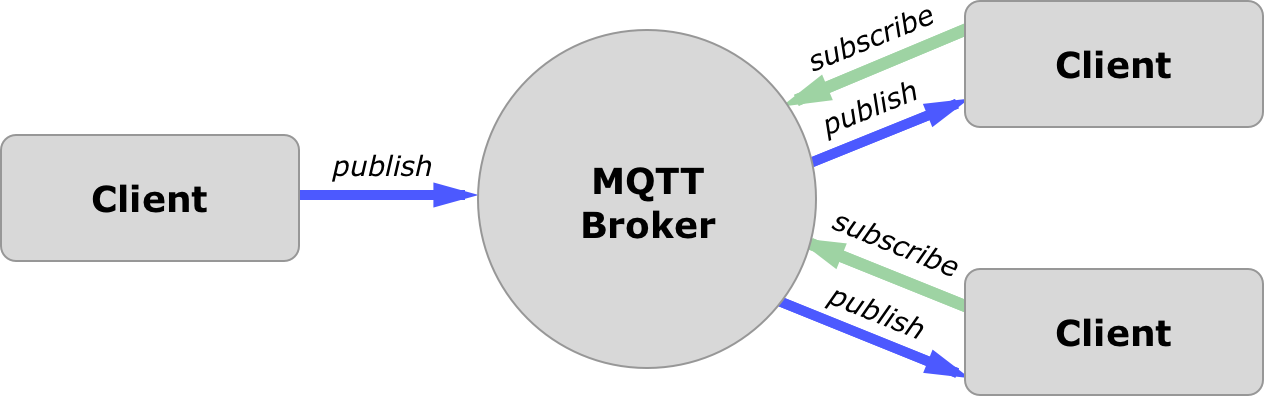
\includegraphics[scale=.25]{./Figures/mqtt-diagram.png}
	\caption{Arquitectura MQTT publish/subscribe.}
	\label{fig:mqttArq}
\end{figure}

La estructura de mensajes en este protocolo se divide en dos: \textit{topics} los cuales son de tipo jerárquicos, utilizando la barra (/) como separador, y \textit{payload} en dónde se incluye el mensaje que se quiere transmitir. Por ejemplo: topic: "nodos/procesos/guardar", payload: "mensaje de ejemplo". Siguiendo este ejemplo un cliente podría suscribirse a ese topic o a una jerarquía más alta y recibir todos los mensajes de los topics que comiencen con nodo/procesos. 

\subsection{Broker Eclipse Mosquitto}
\label{subsec:mosquitto}

Eclipse Mosquitto \citep{WEBSITE:MOSQUITTO} es un broker MQTT \textit{Open Source} liviano y adecuado para utilizar en todo tipo de dispositivos sobre todo aquellos que cuenten con baja potencia como microcontroladores.

El objetivo de Mosquitto es proporcionar una implementación ligera y de bajo consumo de recursos para permitir la comunicación entre dispositivos IoT en redes con ancho de banda limitado y recursos de memoria.

Mosquitto es compatible con una amplia gama de lenguajes de programación, lo que lo hace fácilmente integrable con diferentes aplicaciones. Además, cuenta con una arquitectura flexible y escalable que permite su implementación en dispositivos con diferentes capacidades de procesamiento y memoria.

Otra característica importante de este broker es su capacidad para manejar conexiones seguras a través del uso de protocolos de seguridad como SSL/TLS y SASL. Esto permite la comunicación segura y cifrada entre dispositivos de IoT en diferentes entornos de red.	

\section{Bases de datos}
\label{sec:ddbb}

Las bases de datos son una parte esencial de cualquier aplicación IoT, ya que se utilizan para almacenar y gestionar los datos recopilados por los dispositivos IoT. En esta sección, se describen las tecnologías utilizadas en bases de datos.

\subsection{Bases de datos relacionales}
\label{subsec:RDBMS}

Las bases de datos relacionales \cite{CJ-Date} son un tipo de sistema de gestión de bases de datos (SGBD) que se basa en el modelo de datos relacional. Este modelo se utiliza para organizar y almacenar datos en tablas, donde cada tabla representa una entidad o concepto del mundo real y cada fila representa una instancia de esa entidad.

Las tablas se relacionan entre sí mediante claves primarias y claves externas, lo que permite establecer relaciones entre las entidades y realizar consultas complejas que combinan datos de varias tablas. Además, las bases de datos relacionales utilizan el lenguaje de consulta estructurado (SQL o \textit{Structured Query Language}) para interactuar con los datos almacenados en la base de datos.

En la figura \ref{fig:relddbb} se puede apreciar un ejemplo de un diagrama de base de datos relacional con sus tablas, filas y relaciones.

\begin{figure}[ht]
	\centering
	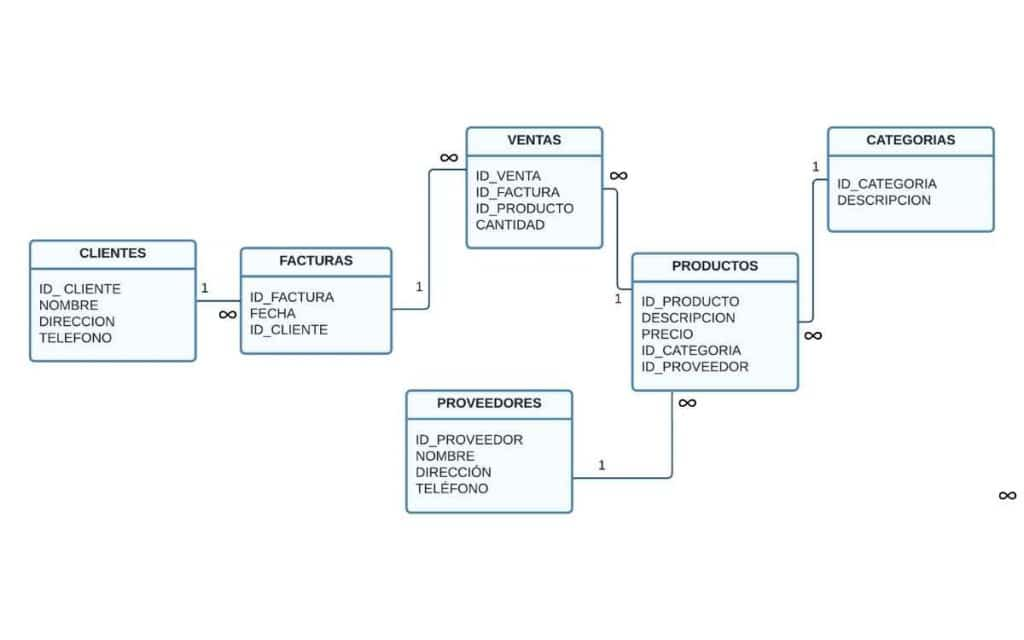
\includegraphics[scale=.30]{./Figures/relddbb.jpg}
	\caption{Diagrama base de datos relacional.}
	\label{fig:relddbb}
\end{figure}

\subsection{Sistema de gestión de base de datos MySQL}
\label{subsec:mysql}

MySQL \citep{WEBSITE:mysql-site} es un sistema de gestión de bases de datos relacional y de código abierto, que utiliza el lenguaje SQL para interactuar con los datos almacenados en la base de datos. 

Ofrece una amplia gama de características avanzadas, como soporte para transacciones ACID, índices avanzados, clústeres de alta disponibilidad y replicación. Además, admite múltiples lenguajes de programación, incluyendo C, C++, Python, Java y Ruby, lo que lo hace extremadamente flexible y escalable.

Tiene múltiples capas de seguridad integradas en el sistema, incluyendo autenticación y control de acceso basado en roles. 

Debido a su combinación de características avanzadas, flexibilidad y seguridad, MySQL se utiliza ampliamente en aplicaciones de misión crítica y de alta disponibilidad, incluyendo aplicaciones IoT.

\section{Tecnologías backend}
\label{sec:backend}

Este tipo de tecnologías se utilizan para desarrollar la lógica de la aplicación y gestionar la comunicación entre el servidor y los dispositivos IoT. En esta sección, se describen las tecnologías backend utilizadas.

\subsection{API RESTFul}
\label{subsec:apis}

Las APIs RESTful \cite{fielding_architectural_2000} \textit{(Representational State Transfer)} son una arquitectura de diseño de aplicaciones web que utiliza el protocolo HTTP para transferir datos. Las API RESTful están diseñadas para ser escalables, flexibles y fáciles de entender para los desarrolladores y los clientes que las consumen.

Están basadas en el concepto de recursos, que son objetos o conjuntos de datos que se pueden acceder a través de una URI (Identificador de recurso uniforme, por sus siglas en inglés). Cada recurso tiene un conjunto de operaciones que se pueden realizar sobre él, como GET (para obtener los datos del recurso), POST (para crear un nuevo recurso), PUT (para actualizar un recurso existente) y DELETE (para eliminar un recurso).

En la figura \ref{fig:apirest} se puede apreciar un ejemplo de una arquitectura API rest, incluyendo la petición o \textit{request} del usuario en formato JSON, el método HTTP y la respuesta o \textit{response} del servidor.

\begin{figure}[ht]
	\centering
	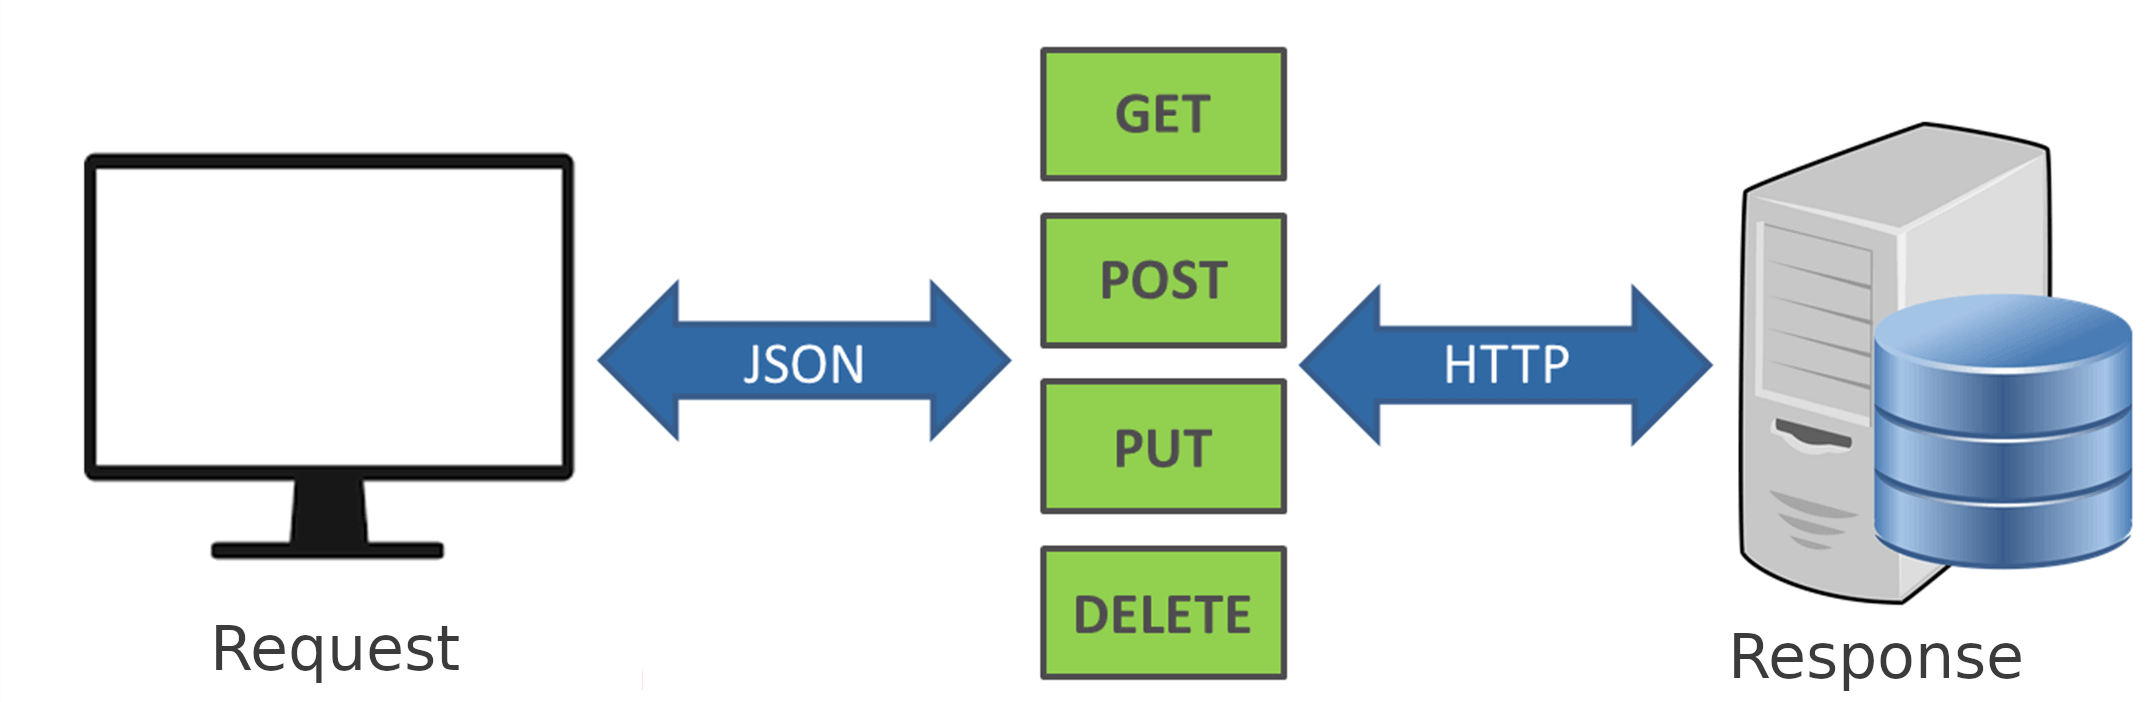
\includegraphics[scale=.15]{./Figures/apirest.png}
	\caption{Arquitectura API Rest.}
	\label{fig:apirest}
\end{figure}

\subsection{Node.js}
\label{subsec:nodejs}

Node.js \cite{WEBSITE:nodejs} es un entorno de tiempo de ejecución de JavaScript de código abierto que se ejecuta en el servidor. Fue creado en 2009 con el objetivo de poder desarrollar aplicaciones escalables y de alto rendimiento utilizando el mismo lenguaje de programación para el lado del servidor y del cliente.

Se basa en el motor de JavaScript V8 de Google, lo que lo hace muy rápido y eficiente. Utiliza un modelo de E/S sin bloqueo y orientado a eventos, lo que significa que es capaz de manejar un gran número de solicitudes simultáneas sin bloquear el proceso. Esto lo hace especialmente adecuado para aplicaciones web en tiempo real y aplicaciones de transmisión de medios.

También cuenta con una amplia variedad de módulos y bibliotecas disponibles a través de su gestor de paquetes NPM (\textit{Node Package Manager}). Esto permite aprovechar funcionalidades existentes, desde la creación de APIs RESTful hasta la manipulación de archivos, la comunicación con dispositivos y bases de datos.

\subsection{Express}
\label{subsec:express}

Express \cite{WEBSITE:express} es un popular framework de Node.js utilizado para la creación de aplicaciones web y APIs RESTful. Fue creado en 2010 y es mantenido por la comunidad de desarrolladores de Node.js.

Proporciona una serie de funcionalidades para simplificar el proceso de creación de aplicaciones web. Entre ellas se incluyen el manejo de rutas, la gestión de middleware, la manipulación de sesiones y cookies, la autenticación de usuarios y la integración con bases de datos.

En Express, el manejo de rutas se realiza mediante la definición estas y los controladores correspondientes. Las rutas son los patrones utilizados para identificar las solicitudes HTTP entrantes que serán atendidas por la aplicación web. Los controladores son las funciones que se encargan de procesar esas solicitudes y generar la respuesta adecuada.

Para definir una ruta, se utiliza el método correspondiente al verbo HTTP que se desea manejar (GET, POST, PUT, DELETE, etc.), seguido de la ruta o patrón que se desea asociar a esa solicitud. 

\subsection{Sequelize}
\label{subsec:sequelize}

Sequelize \cite{WEBSITE:sequelize} es una biblioteca de ORM \textit{(Object-Relational Mapping)} para Node.js que permite trabajar con bases de datos relacionales como MySQL, PostgreSQL, SQLite, y MSSQL. Facilita el acceso a la base de datos y permite la creación de consultas a través de una interfaz de programación de aplicaciones (API) de alto nivel basada en objetos.

Se utiliza junto a Express y Node.js para simplificar el proceso de acceso y manipulación de datos en bases de datos relacionales. Al utilizar Sequelize, se pueden crear modelos de datos que representen las tablas de la base de datos, lo que permite interactuar con la base de datos utilizando objetos en lugar de consultas SQL.

Alguna de las principales ventajas de utilizar Sequelize son:

\begin{itemize}
\item Abstracción de la base de datos: proporciona una abstracción de la base de datos que permite a los desarrolladores trabajar con objetos y métodos en lugar de escribir sentencias SQL. Esto facilita el trabajo con la base de datos y reduce la cantidad de código necesario para realizar operaciones CRUD.

\item Seguridad: proporciona funciones de seguridad incorporadas, como la prevención de inyecciones SQL y la validación de datos de entrada. Esto ayuda a reducir los riesgos de seguridad y garantiza que los datos almacenados en la base de datos sean confiables.

\item Migraciones de base de datos: proporciona una forma fácil de administrar las migraciones de base de datos. Se pueden definir cambios en la estructura de la base de datos utilizando migraciones y aplicarlas en el orden correcto, lo que ayuda a garantizar que la base de datos esté actualizada y que los cambios se realicen de manera controlada.

\item Soporte para múltiples bases de datos: admite múltiples bases de datos, lo que significa que se puede trabajar con diferentes bases de datos sin tener que aprender una nueva sintaxis para cada una. Esto hace que sea más fácil trabajar con diferentes bases de datos y reducir el tiempo de aprendizaje.

\item Integración con Express: se integra bien con Express, lo que permite trabajar con ambos de manera conjunta. Esto hace que sea más fácil construir aplicaciones web y manejar las operaciones de la base de datos al mismo tiempo.

\end{itemize}

\subsection{API messenger}
\label{subsec:apimessenger}

Para el envío de mensajes por la aplicación \textit{WhatsApp} \cite{whatsapp} se utilizó una API adicional \cite{api-whatsapp-ts}, denominada en este trabajo \textit{API Messenger} a fines de distinguirla de la API de \textit{backend} desarrollada.

Esta API presenta un desarrollo en un patrón modular de tipo DDD \textit{(Domain-Driven Design)}. La principal característica en este caso es la creación de capas de infraestructura, servicios y aplicaciones. Esto servirá en caso de cambiar el proveedor de mensajería \textit{WhatsApp} o agregar otro proveedor en paralelo, lo cual hace el sistema escalable y adaptable a diferentes necesidades y escenarios.

Para los requerimientos de este trabajo se personalizó el código fuente de la \textit{API Messenger} a fines de agregar características adicionales, se detalla esto en el capítulo \ref{sec:apimessenger}.

\subsection{Portainer}
\label{subsec:portainer}

Portainer \citep{PortainerDocs} es una herramienta de administración de contenedores Docker \cite{WEBSITE:docker} que proporciona una interfaz web para administrar los contenedores y clústeres Docker. 

Proporciona una variedad de características útiles, incluyendo:

\begin{itemize}
\item Una interfaz web intuitiva y fácil de usar para administrar contenedores Docker, imágenes, volúmenes y redes.
\item La posibilidad de crear y configurar contenedores a través de una interfaz gráfica de usuario (GUI).
\item La gestión de múltiples \textit{hosts} desde una única interfaz de usuario, lo que permite administrar varios clústeres o instancias de Docker en diferentes servidores.
\item La capacidad de ver y administrar fácilmente el estado de los contenedores, así como el uso de recursos y las estadísticas de rendimiento.
\item La gestión de usuarios y roles de acceso, lo que permite controlar el acceso y la autorización de los usuarios.
\item La posibilidad de crear y gestionar \textit{stacks} y servicios de Docker, lo que permite crear aplicaciones complejas y multi-contenedor de manera fácil y rápida.
\end{itemize}

Para este trabajo se utilizó la herramienta solamente para el monitoreo de los contenedores y el control del uso de recursos de sistema de los mismos.

En las figuras \ref{fig:portainer1} y \ref{fig:portainer2} podemos observar la interfaz gráfica de la herramienta.

\begin{figure}[H]
	\centering
	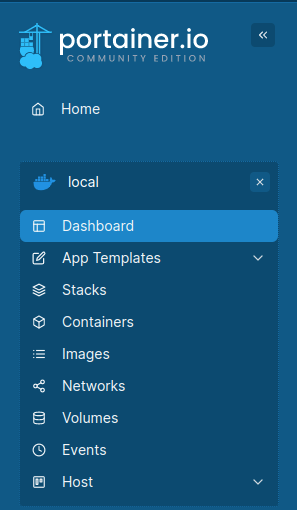
\includegraphics[scale=.20]{./Figures/portainer-admin-1.png}
	\caption{Arquitectura API Rest.}
	\label{fig:portainer1}
\end{figure}

\begin{figure}[H]
	\centering
	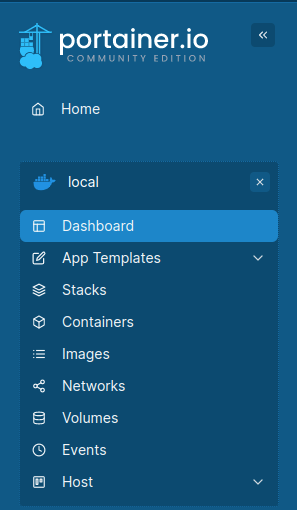
\includegraphics[scale=.20]{./Figures/portainer-admin-1.png}
	\caption{Arquitectura API Rest.}
	\label{fig:portainer2}
\end{figure}


\section{Tecnologías frontend}
\label{sec:frontend}

Las tecnologías frontend son aquellas que se utilizan para crear la parte visual y de interacción de una aplicación web o móvil. Estas tecnologías se enfocan en la presentación y manipulación de la interfaz de usuario, en la interacción con el usuario final y actúa como intermediario entre el usuario final y el backend de la aplicación.

Algunas de las tecnologías frontend más comunes son:
\begin{itemize}
	\item HTML \cite{WEBSITE:HTML} \textit{(HyperText Markup Language)}: es el lenguaje de marcado que se utiliza para estructurar y dar formato al contenido de una página web.
	\item CSS \cite{WEBSITE:css} \textit{(Cascading Style Sheets)}: es el lenguaje utilizado para dar estilo y diseño a una página web, permitiendo la personalización de fuentes, colores, márgenes, tamaños y otros aspectos visuales.
	\item JavaScript \cite{WEBSITE:javascript}: es un lenguaje de programación que se utiliza para hacer que la página web sea interactiva y dinámica, permitiendo la manipulación de elementos del DOM \cite{WEBSITE:DOM} \textit{(Document Object Model)}, eventos, animaciones y otras acciones en el lado del cliente.
	\item Frameworks de JavaScript: son bibliotecas que permiten simplificar el desarrollo de aplicaciones web, proporcionando funcionalidades predefinidas y estructuras de organización.
	\item Bibliotecas de diseño: son herramientas que ofrecen componentes visuales predefinidos y estilos de diseño que permiten crear páginas web con un aspecto más profesional y elegante.
	\item Herramientas de gestión de paquetes: son programas que permiten gestionar las dependencias de los proyectos y mantener actualizadas las librerías utilizadas en el desarrollo.	
\end{itemize}

\subsection{Ionic framework}
\label{subsec:ionic}

Ionic \cite{WEBSITE:ionic} es un framework de desarrollo de aplicaciones móviles híbridas basado en tecnologías web como HTML, CSS y JavaScript. Permite crear aplicaciones móviles para iOS, Android y la web utilizando un conjunto de herramientas y bibliotecas predefinidas.

Ofrece una gran cantidad de componentes visuales, animaciones y funcionalidades para crear aplicaciones móviles con una apariencia y experiencia de usuario nativa, similar a las aplicaciones desarrolladas con tecnologías nativas como Java para Android o Swift para iOS. Además, permite la integración con otras tecnologías como Angular \cite{WEBSITE:angular} y React \cite{WEBSITE:react}.

El uso de tecnologías web permite el desarrollo de aplicaciones móviles de forma más rápida y sencilla que las aplicaciones nativas, ya que se utiliza un único código base que se puede adaptar para cada plataforma. Además, ofrece una gran cantidad de herramientas y servicios para simplificar el proceso de desarrollo, como Ionic Native (para el acceso a las características nativas del dispositivo) y Ionic Appflow (para la implementación continua y la gestión de versiones).

%En resumen, Ionic es una herramienta muy útil para el desarrollo de aplicaciones móviles híbridas utilizando tecnologías web, que permite crear aplicaciones con una apariencia y experiencia de usuario nativa, y que simplifica el proceso de desarrollo gracias a su conjunto de herramientas y servicios predefinidos.

\section{Tecnologías de servidor}
\label{sec:servidor}

\subsection{Docker y Docker Compose}
\label{subsec:docker}

Docker \cite{WEBSITE:docker} es una plataforma de software libre que se utiliza para desarrollar, implementar y ejecutar aplicaciones en contenedores. Los contenedores son una forma de virtualización que permiten a los desarrolladores empaquetar una aplicación y todas sus dependencias en una imagen de contenedor, que se puede ejecutar en cualquier entorno que tenga Docker instalado. Docker facilita la implementación de aplicaciones en diferentes plataformas, desde servidores locales hasta nubes públicas.

Docker Compose \cite{WEBSITE:docker-compose} es una herramienta de Docker que se utiliza para definir y ejecutar aplicaciones de múltiples contenedores. Permite definir todos los servicios necesarios para una aplicación en un archivo de configuración YAML, lo que facilita la implementación y el mantenimiento de la aplicación. Docker Compose puede iniciar todos los contenedores necesarios para la aplicación con un solo comando, lo que ahorra tiempo y reduce los errores.

\subsection{Servidor web Nginx}
\label{subsec:servidorweb}

Un servidor web es un software que procesa solicitudes HTTP de clientes y responde con contenido estático o dinámico. Los servidores web se utilizan para alojar y servir sitios web y aplicaciones web. Un servidor web típicamente aloja varios sitios web y puede gestionar múltiples solicitudes HTTP simultáneamente.

Nginx \cite{WEBSITE:NGINX} es un servidor web de código abierto que se utiliza para alojar y servir sitios web y aplicaciones web. Nginx es conocido por su alta escalabilidad, rendimiento y capacidad de manejar múltiples solicitudes HTTP simultáneamente. Es un servidor web ligero y rápido que se puede utilizar como un proxy inverso para distribuir la carga de trabajo a diferentes servidores y balancear la carga de tráfico.

\section{Hardware utilizado}
\label{sec:hardware}

\subsection{Raspberry Pi}
\label{subsec:rbpi}

La Raspberry Pi \cite{WEBSITE:raspberrypi} es una pequeña computadora de placa única (\textit{Simple Board Computer}, por sus siglas en inglés) diseñada para ser utilizada en proyectos de tecnología, educación y prototipos de hardware. Fue desarrollada por la Fundación Raspberry Pi, una organización benéfica con sede en el Reino Unido.

Principales características del modelo Raspberry Pi 4 seleccionado para este trabajo:

\begin{itemize}
\item Procesador Broadcom BCM2711 de cuatro núcleos ARM Cortex-A72 a 1,5 GHz.
\item Procesador gráfico VideoCore VI con soporte para OpenGL ES 3.x. 
\item 8 GB de memoria RAM LPDDR4-3200.
\item Bluetooth 5.0.
\item Wi-Fi de doble banda 802.11ac.
\item Gigabit Ethernet.
\end{itemize}

Puertos:
\begin{itemize}
\item Dos puertos micro-HDMI que pueden soportar dos pantallas con resolución de hasta 4K a 60 fps.
\item Dos puertos USB 3.0.
\item Dos puertos USB 2.0
\item Un puerto GPIO de 40 pines
\item Un puerto CSI para la conexión de una cámara
\item Un puerto DSI para la conexión de una pantalla táctil
\item Un puerto de audio de 3,5 mm.
\end{itemize}

La placa es compatible con diferentes sistemas operativos, incluyendo Raspberry Pi OS (anteriormente llamado Raspbian), Ubuntu, Windows 10 IoT Core y otros sistemas operativos basados en Linux. También es compatible con diferentes lenguajes de programación como Python, C++, Java y más, lo que la hace ideal para proyectos de IoT, robótica, automatización del hogar, entre otros.

\subsection{NodeMCU Esp32}
\label{subsec:esp32}

La NodeMCU ESP32 \cite{ESP32-DOC} es una placa de desarrollo basada en el microcontrolador ESP32, que es ampliamente utilizado en proyectos de Internet de las cosas (IoT). 

Detalles técnicos del modelo NodeMCU ESP32 WROOM 32 seleccionado para este trabajo:

\begin{itemize}
\item Microcontrolador ESP32 de doble núcleo con una velocidad de reloj de hasta 240 MHz y 512 kB de memoria RAM.
\item 4 MB de memoria flash integrada para almacenamiento de programas y datos.
\item Conectividad inalámbrica Wi-Fi 802.11 b/g/n y Bluetooth 4.2 BLE.
\item Interfaz de programación USB integrada para programar la placa y proporcionar una conexión de depuración.
\item GPIO de 30 pines para la conexión de sensores, actuadores y otros dispositivos periféricos.
\item Interfaces I2C, SPI, UART, PWM y ADC integradas.
\item Soporte para el entorno de programación Arduino, así como para MicroPython y Lua.
\item Compatible con una amplia gama de bibliotecas y herramientas de desarrollo de código abierto.
\end{itemize}

\subsection{Identificación por radiofrecuencia}
\label{subsec:rfid}

RFID \cite{RFID} son las siglas en inglés de \textit{Radio Frequency Identification} o identificación por radiofrecuencia en español. Es una tecnología de identificación automática que utiliza ondas de radio para leer y capturar información almacenada en etiquetas o \textit{tags} RFID.

Esta tecnología consta de tres componentes básicos: el tag RFID que comunmente es una tarjeta o llavero pequeño, el lector RFID y un sistema informático que gestiona la información capturada por el lector. 

Los tags RFID contienen antenas y circuitos integrados que permiten la comunicación inalámbrica con los lectores, los cuales envían señales de radio para alimentar y activar los tags, y recibir la información almacenada en ellos. Pueden ser pasivos, activos o semi-activos, dependiendo de si necesitan o no una fuente de alimentación externa. 


\subsection{Módulo RC522}
\label{subsec:rc522}


El RFID RC522 \cite{MFRC522} es un módulo de lectura-escritura RFID que utiliza la tecnología de comunicación de campo cercano (NFC) para la identificación y el intercambio de datos de manera inalámbrica. Entre sus principales características se encuentran:

\begin{itemize}
\item Soporte para frecuencias de operación de 13,56 MHz.
\item Comunicación mediante el protocolo SPI \textit{(Serial Peripheral Interface)}.
\item Capacidad para leer y escribir etiquetas RFID de tipo MIFARE, que son ampliamente utilizadas en sistemas de acceso, control de inventario, pago sin contacto, entre otros.
\item Funciones de autenticación y encriptación para mayor seguridad en la transmisión de datos.
\item Bajo consumo de energía y fácil integración con microcontroladores y otros sistemas embebidos.
\end{itemize}

\subsection{Buzzer sonoro}
\label{subsec:buzzer}

El módulo buzzer pasivo KY006 \cite{BUZZER} es un pequeño dispositivo electrónico que se utiliza para producir sonidos audibles en una variedad de proyectos electrónicos. Se conecta a la placa de control mediante tres pines.

Entre las características técnicas del módulo KY006 se encuentran:

\begin{itemize}
\item Tensión de funcionamiento: 5 V DC.
\item Corriente de funcionamiento: < 25 mA.
\item Tipo de sonido: continuo y monótono.
\item Frecuencia de resonancia: 2300 ± 300 Hz.
\item SPL (nivel de presión sonora): > 85 dB a 10 cm de distancia.
\item Diámetro: 30 mm.
\item Altura: 7,5 mm.
\item Peso: 4 gramos.
\end{itemize}


%Se recomienda no utilizar \textbf{texto en negritas} en ningún párrafo, ni tampoco texto \underline{subrayado}. En cambio sí se debe utilizar \textit{texto en itálicas} para palabras en un idioma extranjero, al menos la primera vez que aparecen en el texto. En el caso de palabras que estamos inventando se deben utilizar ``comillas'', así como también para citas textuales. Por ejemplo, un \textit{digital filter} es una especie de ``selector'' que permite separar ciertos componentes armónicos en particular.
%
%La escritura debe ser impersonal. Por ejemplo, no utilizar ``el diseño del firmware lo hice de acuerdo con tal principio'', sino ``el firmware fue diseñado utilizando tal principio''. 
%
%El trabajo es algo que al momento de escribir la memoria se supone que ya está concluido, entonces todo lo que se refiera a hacer el trabajo se narra en tiempo pasado, porque es algo que ya ocurrió. Por ejemplo, "se diseñó el firmware empleando la técnica de test driven development".
%
%En cambio, la memoria es algo que está vivo cada vez que el lector la lee. Por eso transcurre siempre en tiempo presente, como por ejemplo:
%
%``En el presente capítulo se da una visión global sobre las distintas pruebas realizadas y los resultados obtenidos. Se explica el modo en que fueron llevados a cabo los test unitarios y las pruebas del sistema''.
%
%Se recomienda no utilizar una sección de glosario sino colocar la descripción de las abreviaturas como parte del mismo cuerpo del texto. Por ejemplo, RTOS (\textit{Real Time Operating System}, Sistema Operativo de Tiempo Real) o en caso de considerarlo apropiado mediante notas a pie de página.
%
%Si se desea indicar alguna página web utilizar el siguiente formato de referencias bibliográficas, dónde las referencias se detallan en la sección de bibliografía de la memoria, utilizado el formato establecido por IEEE en \citep{IEEE:citation}. Por ejemplo, ``el presente trabajo se basa en la plataforma EDU-CIAA-NXP \citep{CIAA}, la cual...''.
%
%\subsection{Figuras} 
%
%Al insertar figuras en la memoria se deben considerar determinadas pautas. Para empezar, usar siempre tipografía claramente legible. Luego, tener claro que \textbf{es incorrecto} escribir por ejemplo esto: ``El diseño elegido es un cuadrado, como se ve en la siguiente figura:''
%
%\begin{figure}[h]
%\centering
%\includegraphics[scale=.45]{./Figures/cuadradoAzul.png}
%\end{figure}
%
%La forma correcta de utilizar una figura es con referencias cruzadas, por ejemplo: ``Se eligió utilizar un cuadrado azul para el logo, como puede observarse en la figura \ref{fig:cuadradoAzul}''.
%
%\begin{figure}[ht]
%	\centering
%	\includegraphics[scale=.45]{./Figures/cuadradoAzul.png}
%	\caption{Ilustración del cuadrado azul que se eligió para el diseño del logo.\protect\footnotemark.}
%	\label{fig:cuadradoAzul}
%\end{figure}
%
%\footnotetext{Imagen tomada de \url{https://goo.gl/images/i7C70w}}
%
%
%El texto de las figuras debe estar siempre en español, excepto que se decida reproducir una figura original tomada de alguna referencia. En ese caso la referencia de la cual se tomó la figura debe ser indicada en el epígrafe de la figura e incluida como una nota al pie, como se ilustra en la figura \ref{fig:palabraIngles}.
%
%\begin{figure}[htpb]
%	\centering
%	\includegraphics[scale=.3]{./Figures/word.jpeg}
%	\caption{Imagen tomada de la página oficial del procesador\protect\footnotemark.}
%	\label{fig:palabraIngles}
%\end{figure}
%
%\footnotetext{Imagen tomada de \url{https://goo.gl/images/i7C70w}}
%
%La figura y el epígrafe deben conformar una unidad cuyo significado principal pueda ser comprendido por el lector sin necesidad de leer el cuerpo central de la memoria. Para eso es necesario que el epígrafe sea todo lo detallado que corresponda y si en la figura se utilizan abreviaturas entonces aclarar su significado en el epígrafe o en la misma figura.
%
%
%
%\begin{figure}[ht]
%	\centering
%	\includegraphics[scale=.37]{./Figures/questionMark.png}
%	\caption{¿Por qué de pronto aparece esta figura?}
%	\label{fig:questionMark}
%\end{figure}
%
%Nunca colocar una figura en el documento antes de hacer la primera referencia a ella, como se ilustra con la figura \ref{fig:questionMark}, porque sino el lector no comprenderá por qué de pronto aparece la figura en el documento, lo que distraerá su atención.
%
%Otra posibilidad es utilizar el entorno \textit{subfigure} para incluir más de una figura, como se puede ver en la figura \ref{fig:three graphs}. Notar que se pueden referenciar también las figuras internas individualmente de esta manera: \ref{fig:1de3}, \ref{fig:2de3} y \ref{fig:3de3}.
% 
%\begin{figure}[!htpb]
%     \centering
%     \begin{subfigure}[b]{0.3\textwidth}
%         \centering
%         \includegraphics[width=.65\textwidth]{./Figures/questionMark}
%         \caption{Un caption.}
%         \label{fig:1de3}
%     \end{subfigure}
%     \hfill
%     \begin{subfigure}[b]{0.3\textwidth}
%         \centering
%         \includegraphics[width=.65\textwidth]{./Figures/questionMark}
%         \caption{Otro.}
%         \label{fig:2de3}
%     \end{subfigure}
%     \hfill
%     \begin{subfigure}[b]{0.3\textwidth}
%         \centering
%         \includegraphics[width=.65\textwidth]{./Figures/questionMark}
%         \caption{Y otro más.}
%         \label{fig:3de3}
%     \end{subfigure}
%        \caption{Tres gráficos simples}
%        \label{fig:three graphs}
%\end{figure}
%
%El código para generar las imágenes se encuentra disponible para su reutilización en el archivo \file{Chapter2.tex}.
%
%\subsection{Tablas}
%
%Para las tablas utilizar el mismo formato que para las figuras, sólo que el epígrafe se debe colocar arriba de la tabla, como se ilustra en la tabla \ref{tab:peces}. Observar que sólo algunas filas van con líneas visibles y notar el uso de las negritas para los encabezados.  La referencia se logra utilizando el comando \verb|\ref{<label>}| donde label debe estar definida dentro del entorno de la tabla.
%
%\begin{verbatim}
%\begin{table}[h]
%	\centering
%	\caption[caption corto]{caption largo más descriptivo}
%	\begin{tabular}{l c c}    
%		\toprule
%		\textbf{Especie}     & \textbf{Tamaño} & \textbf{Valor}\\
%		\midrule
%		Amphiprion Ocellaris & 10 cm           & \$ 6.000 \\		
%		Hepatus Blue Tang    & 15 cm           & \$ 7.000 \\
%		Zebrasoma Xanthurus  & 12 cm           & \$ 6.800 \\
%		\bottomrule
%		\hline
%	\end{tabular}
%	\label{tab:peces}
%\end{table}
%\end{verbatim}
%
%
%\begin{table}[h]
%	\centering
%	\caption[caption corto]{caption largo más descriptivo}
%	\begin{tabular}{l c c}    
%		\toprule
%		\textbf{Especie} 	 & \textbf{Tamaño} 		& \textbf{Valor}  \\
%		\midrule
%		Amphiprion Ocellaris & 10 cm 				& \$ 6.000 \\		
%		Hepatus Blue Tang	 & 15 cm				& \$ 7.000 \\
%		Zebrasoma Xanthurus	 & 12 cm				& \$ 6.800 \\
%		\bottomrule
%		\hline
%	\end{tabular}
%	\label{tab:peces}
%\end{table}
%
%En cada capítulo se debe reiniciar el número de conteo de las figuras y las tablas, por ejemplo, figura 2.1 o tabla 2.1, pero no se debe reiniciar el conteo en cada sección. Por suerte la plantilla se encarga de esto por nosotros.
%
%\subsection{Ecuaciones}
%\label{sec:Ecuaciones}
%
%Al insertar ecuaciones en la memoria dentro de un entorno \textit{equation}, éstas se numeran en forma automática  y se pueden referir al igual que como se hace con las figuras y tablas, por ejemplo ver la ecuación \ref{eq:metric}.
%
%\begin{equation}
%	\label{eq:metric}
%	ds^2 = c^2 dt^2 \left( \frac{d\sigma^2}{1-k\sigma^2} + \sigma^2\left[ d\theta^2 + \sin^2\theta d\phi^2 \right] \right)
%\end{equation}
%                                                        
%Es importante tener presente que si bien las ecuaciones pueden ser referidas por su número, también es correcto utilizar los dos puntos, como por ejemplo ``la expresión matemática que describe este comportamiento es la siguiente:''
%
%\begin{equation}
%	\label{eq:schrodinger}
%	\frac{\hbar^2}{2m}\nabla^2\Psi + V(\mathbf{r})\Psi = -i\hbar \frac{\partial\Psi}{\partial t}
%\end{equation}
%
%Para generar la ecuación \ref{eq:metric} se utilizó el siguiente código:
%
%\begin{verbatim}
%\begin{equation}
%	\label{eq:metric}
%	ds^2 = c^2 dt^2 \left( \frac{d\sigma^2}{1-k\sigma^2} + 
%	\sigma^2\left[ d\theta^2 + 
%	\sin^2\theta d\phi^2 \right] \right)
%\end{equation}
%\end{verbatim}
%
%Y para la ecuación \ref{eq:schrodinger}:
%
%\begin{verbatim}
%\begin{equation}
%	\label{eq:schrodinger}
%	\frac{\hbar^2}{2m}\nabla^2\Psi + V(\mathbf{r})\Psi = 
%	-i\hbar \frac{\partial\Psi}{\partial t}
%\end{equation}
%
%\end{verbatim} 
%	\chapter{Diseño e implementación} % Main chapter title

\label{Chapter3} % Change X to a consecutive number; for referencing this chapter elsewhere, use \ref{ChapterX}

\definecolor{mygreen}{rgb}{0,0.6,0}
\definecolor{mygray}{rgb}{0.5,0.5,0.5}
\definecolor{mymauve}{rgb}{0.58,0,0.82}

%%%%%%%%%%%%%%%%%%%%%%%%%%%%%%%%%%%%%%%%%%%%%%%%%%%%%%%%%%%%%%%%%%%%%%%%%%%%%
% parámetros para configurar el formato del código en los entornos lstlisting
%%%%%%%%%%%%%%%%%%%%%%%%%%%%%%%%%%%%%%%%%%%%%%%%%%%%%%%%%%%%%%%%%%%%%%%%%%%%%
\lstset{ %
  backgroundcolor=\color{white},   % choose the background color; you must add \usepackage{color} or \usepackage{xcolor}
  basicstyle=\footnotesize,        % the size of the fonts that are used for the code
  breakatwhitespace=false,         % sets if automatic breaks should only happen at whitespace
  breaklines=true,                 % sets automatic line breaking
  captionpos=b,                    % sets the caption-position to bottom
  commentstyle=\color{mygreen},    % comment style
  deletekeywords={...},            % if you want to delete keywords from the given language
  %escapeinside={\%*}{*)},          % if you want to add LaTeX within your code
  %extendedchars=true,              % lets you use non-ASCII characters; for 8-bits encodings only, does not work with UTF-8
  %frame=single,	                % adds a frame around the code
  keepspaces=true,                 % keeps spaces in text, useful for keeping indentation of code (possibly needs columns=flexible)
  keywordstyle=\color{blue},       % keyword style
  language=[ANSI]C,                % the language of the code
  %otherkeywords={*,...},           % if you want to add more keywords to the set
  numbers=left,                    % where to put the line-numbers; possible values are (none, left, right)
  numbersep=5pt,                   % how far the line-numbers are from the code
  numberstyle=\tiny\color{mygray}, % the style that is used for the line-numbers
  rulecolor=\color{black},         % if not set, the frame-color may be changed on line-breaks within not-black text (e.g. comments (green here))
  showspaces=false,                % show spaces everywhere adding particular underscores; it overrides 'showstringspaces'
  showstringspaces=false,          % underline spaces within strings only
  showtabs=false,                  % show tabs within strings adding particular underscores
  stepnumber=1,                    % the step between two line-numbers. If it's 1, each line will be numbered
  stringstyle=\color{mymauve},     % string literal style
  tabsize=2,	                   % sets default tabsize to 2 spaces
  title=\lstname,                  % show the filename of files included with \lstinputlisting; also try caption instead of title
  morecomment=[s]{/*}{*/}
}


%----------------------------------------------------------------------------------------
%	SECTION 1
%----------------------------------------------------------------------------------------
\section{Arquitectura general del sistema}
\label{sec:arquitecturagral}

\subsection{Funcionamiento}
\label{subsec:funcionamiento}
Como se puede observar en la figura \ref{fig:diagramafunciones}, el sistema está compuesto por nodos, los cuales se utilizan para la lectura de tarjetas RFID asignadas a los repuestos de los clientes. Los datos se transmiten en una red local, se procesan y almacenan en un servidor con base de datos y son consultados desde la aplicación web en las terminales (\textit{PC} o \textit{smartphone}).

\begin{figure}[H]
	\centering
	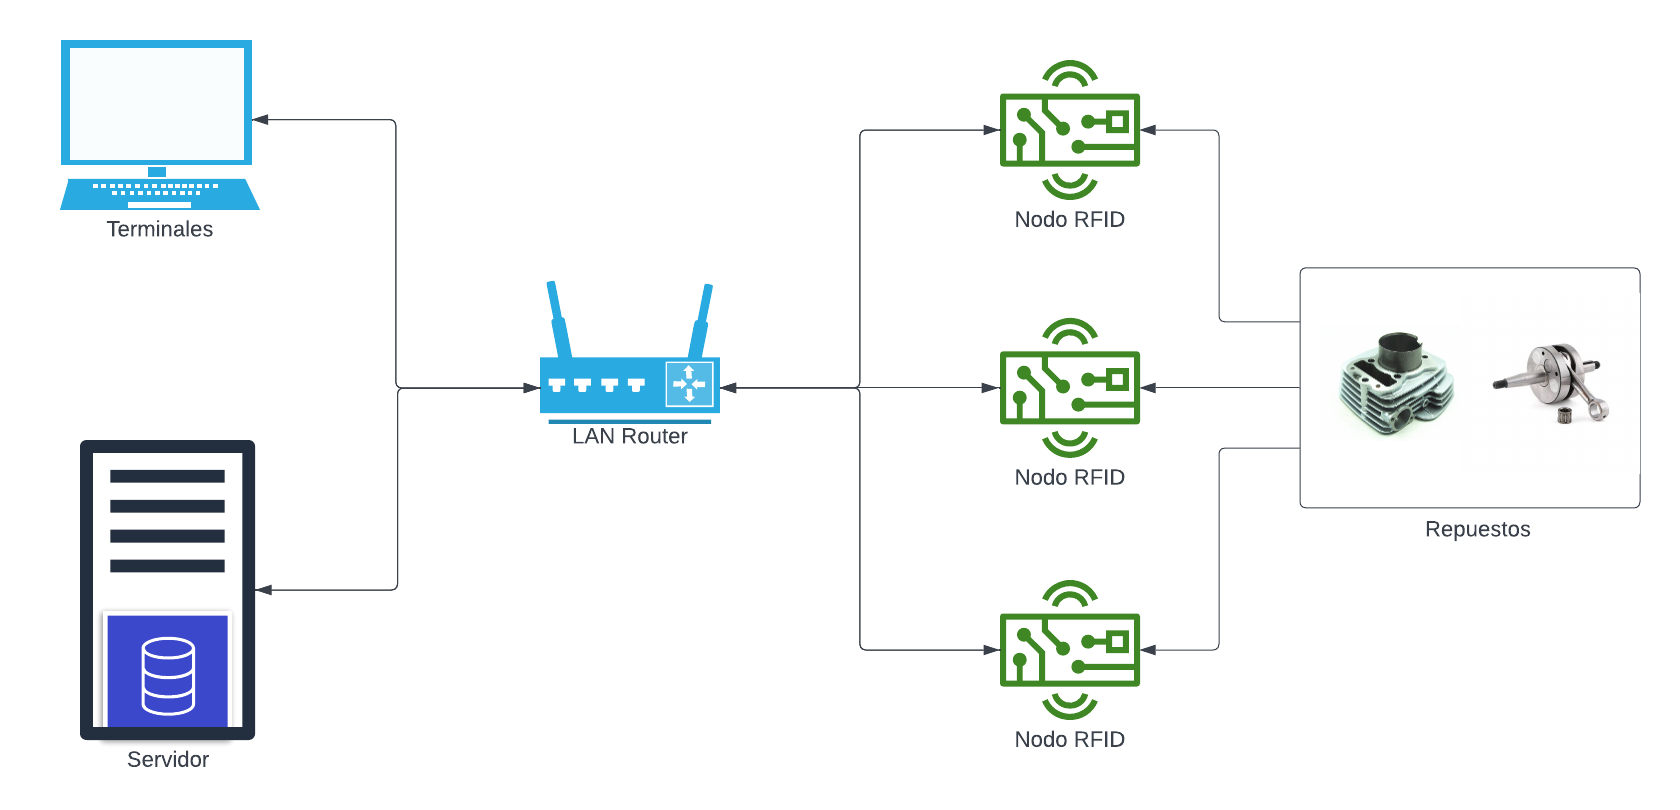
\includegraphics[width=\textwidth]{./Figures/diagramafunciones.png}
	\caption{Diagrama de funciones generales.}
	\label{fig:diagramafunciones}
\end{figure}

\subsection{Diagrama de bloques}
\label{subsec:diagramabloques}
En la figura \ref{fig:diagramabloques} se representa el patrón de modelo conceptual empleado y las tecnologías que se utilizan en cada capa. Se implementó un modelo de 4 capas: 

\begin{itemize}
\item Capa de percepción.
\item Capa de transporte.
\item Capa de procesamiento.
\item Capa de aplicación.
\end{itemize}


\begin{figure}[H]
	\centering
	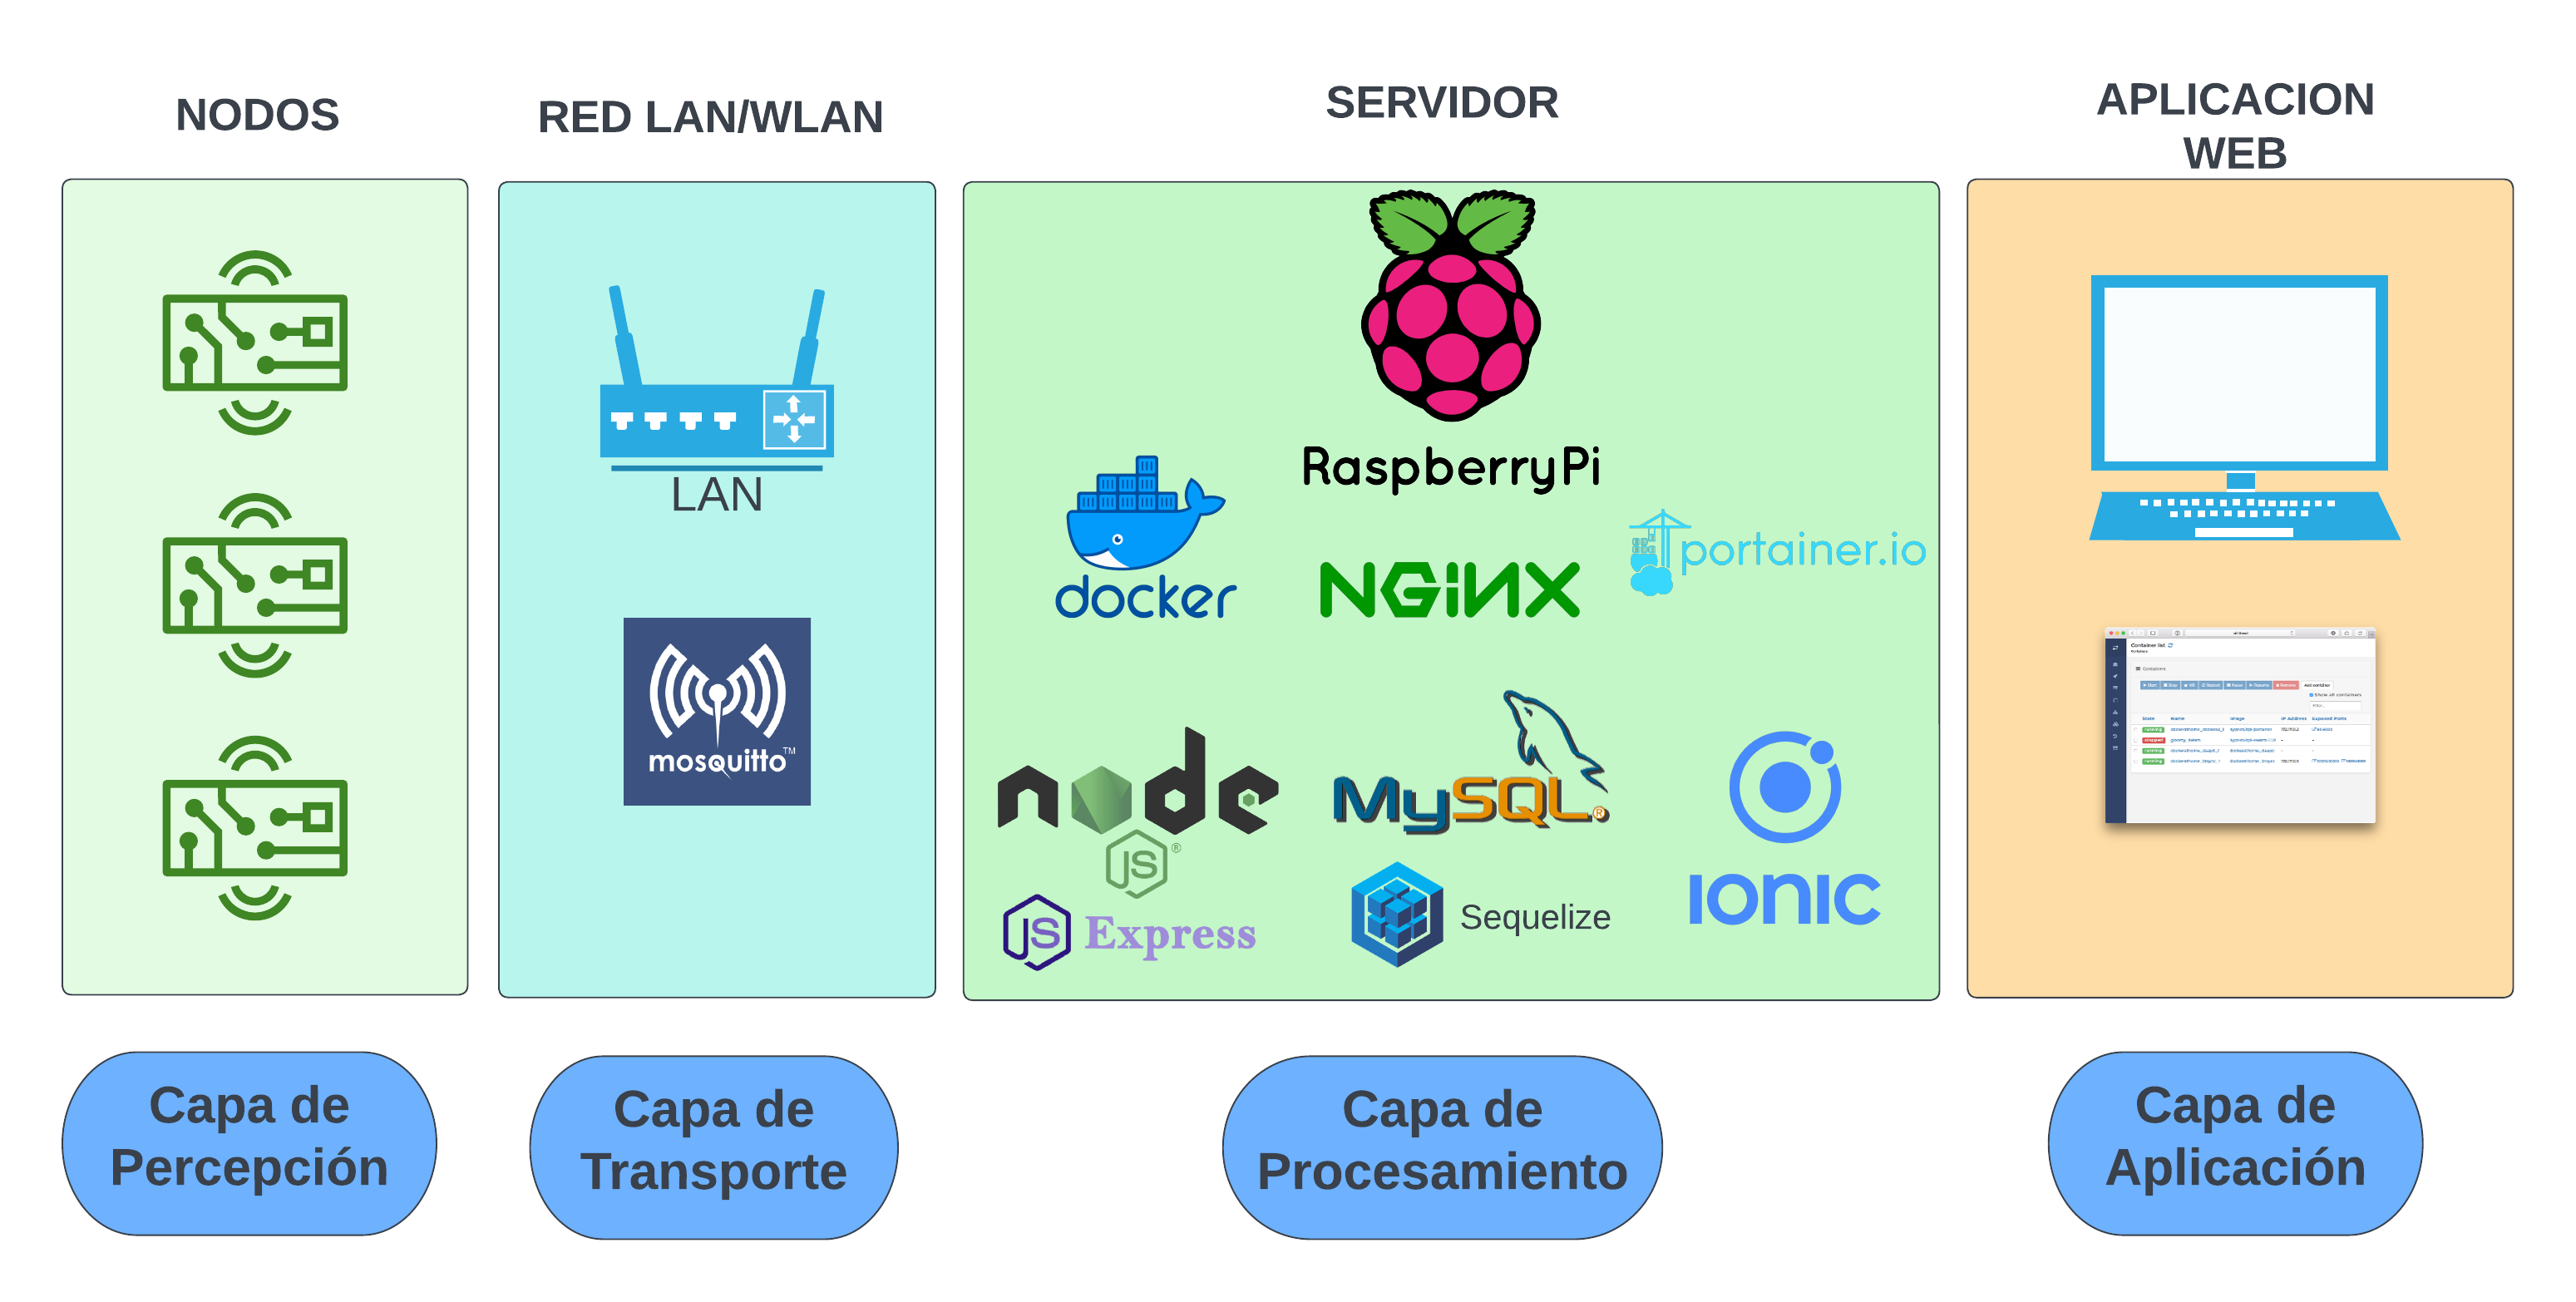
\includegraphics[width=\textwidth]{./Figures/diagramabloques.png}
	\caption{Diagrama de bloques y tecnologías del sistema.}
	\label{fig:diagramabloques}
\end{figure}


En la capa de percepción se utilizan los nodos ESP32 con lector RFID con los cuales se realiza la lectura de las tarjetas correspondientes. Una vez realizada la lectura, los datos son enviados por medio del protocolo MQTT y a través de la red local en la capa de transporte. 

La capa de transporte es la encargada de transmitir los mensajes por medio de los protocolos MQTT y HTTP. El \textit{broker} Eclipse Mosquitto distribuye los mensajes publicados a los suscriptores para su procesamiento.

En la capa de procesamiento se realiza la lógica del backend, la base de datos y el frontend. Se implementó un servidor central en una Raspberry Pi 4 con todos los servicios. Cada uno de los servicios está desarrollado de manera individual y fue montado en su propio contenedor de Docker. Todos los contenedores se despliegan utilizando Docker Compose.

Por último, la capa de aplicación otorga el acceso web, desarrollado en el \textit{framework } \textit{Ionic}, para el ingreso, registro, administración y egreso de las ordenes de trabajo. También se utiliza el portal de administración de \textit{Portainer} para el monitoreo completo de Docker y del servidor.


\section{Flujo general del sistema}
\label{sec:flujogeneral}
En esta sección se explica el flujo total de las funciones del sistema desde que el usuario ingresa una nueva orden de trabajo hasta que el producto es retirado por el cliente.

Las comunicaciones y el envío de datos entre los distintos módulos del sistema se realizan en los protocolos HTTP, MQTT y MySQL. Se detallará en cada caso el protocolo utilizado.

\subsection{Ingreso de repuesto}
\label{subsec:ingresorepuesto}
En la figura \ref{fig:flujoingreso} se puede observar todos los módulos del sistema, el flujo de datos y protocolos que intervienen cuando un usuario carga una nueva orden de trabajo en el sistema.

\begin{figure}[ht]
	\centering
	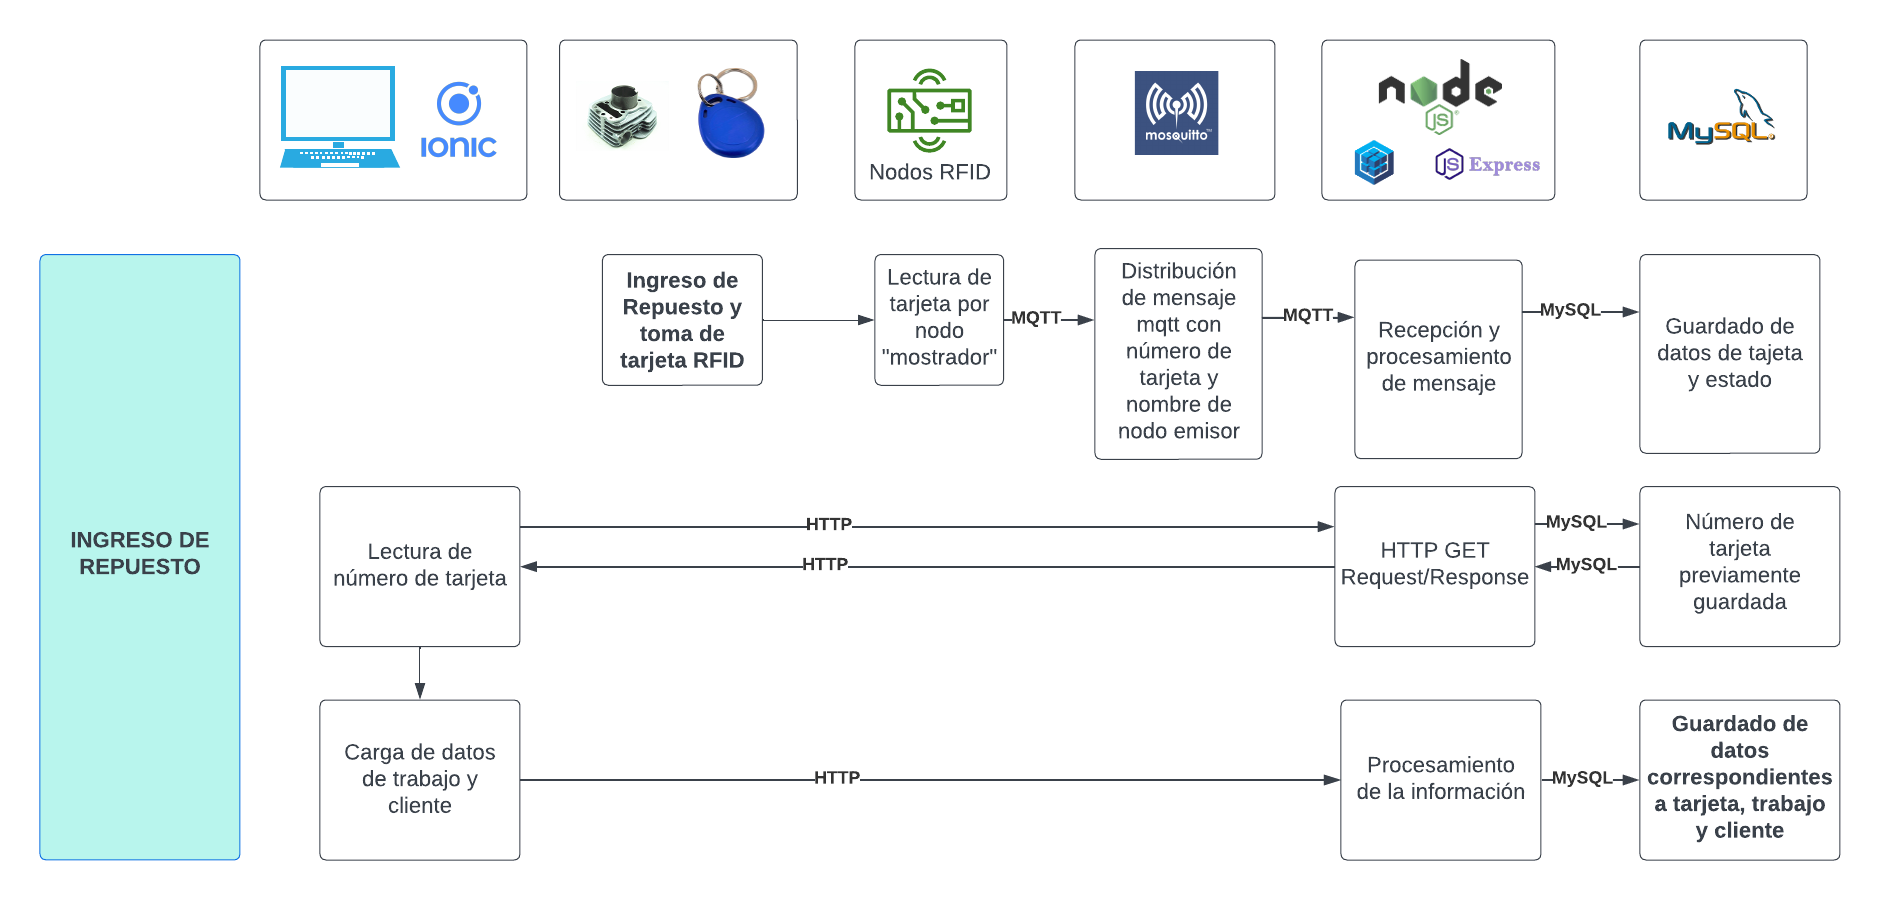
\includegraphics[width=\textwidth]{./Figures/flujoingreso.png}
	\caption{Flujo en el ingreso de una nueva orden de trabajo.}
	\label{fig:flujoingreso}
\end{figure}
  
El flujo inicia cuando el usuario recibe el repuesto y selecciona una tarjeta RFID libre para usarla con ese repuesto. El usuario pasa la tarjeta por el nodo ubicado en la recepción, nodo mostrador, y de esta manera se registra el número de tarjeta para ser utilizada. Luego el usuario carga los datos en la aplicación web, dónde ya está asignada la tarjeta previamente leída, confirma los datos y estos son guardados en la base de datos. La nueva orden de trabajo tiene su número de tarjeta, los datos del cliente y el estado por defecto en espera.

\subsection{Cambio de estado}
\label{subsec:flujocambioestado}

En la figura \ref{fig:flujocambioestado} se representa el flujo completo para un cambio de estado de una orden de trabajo.

\begin{figure}[ht]
	\centering
	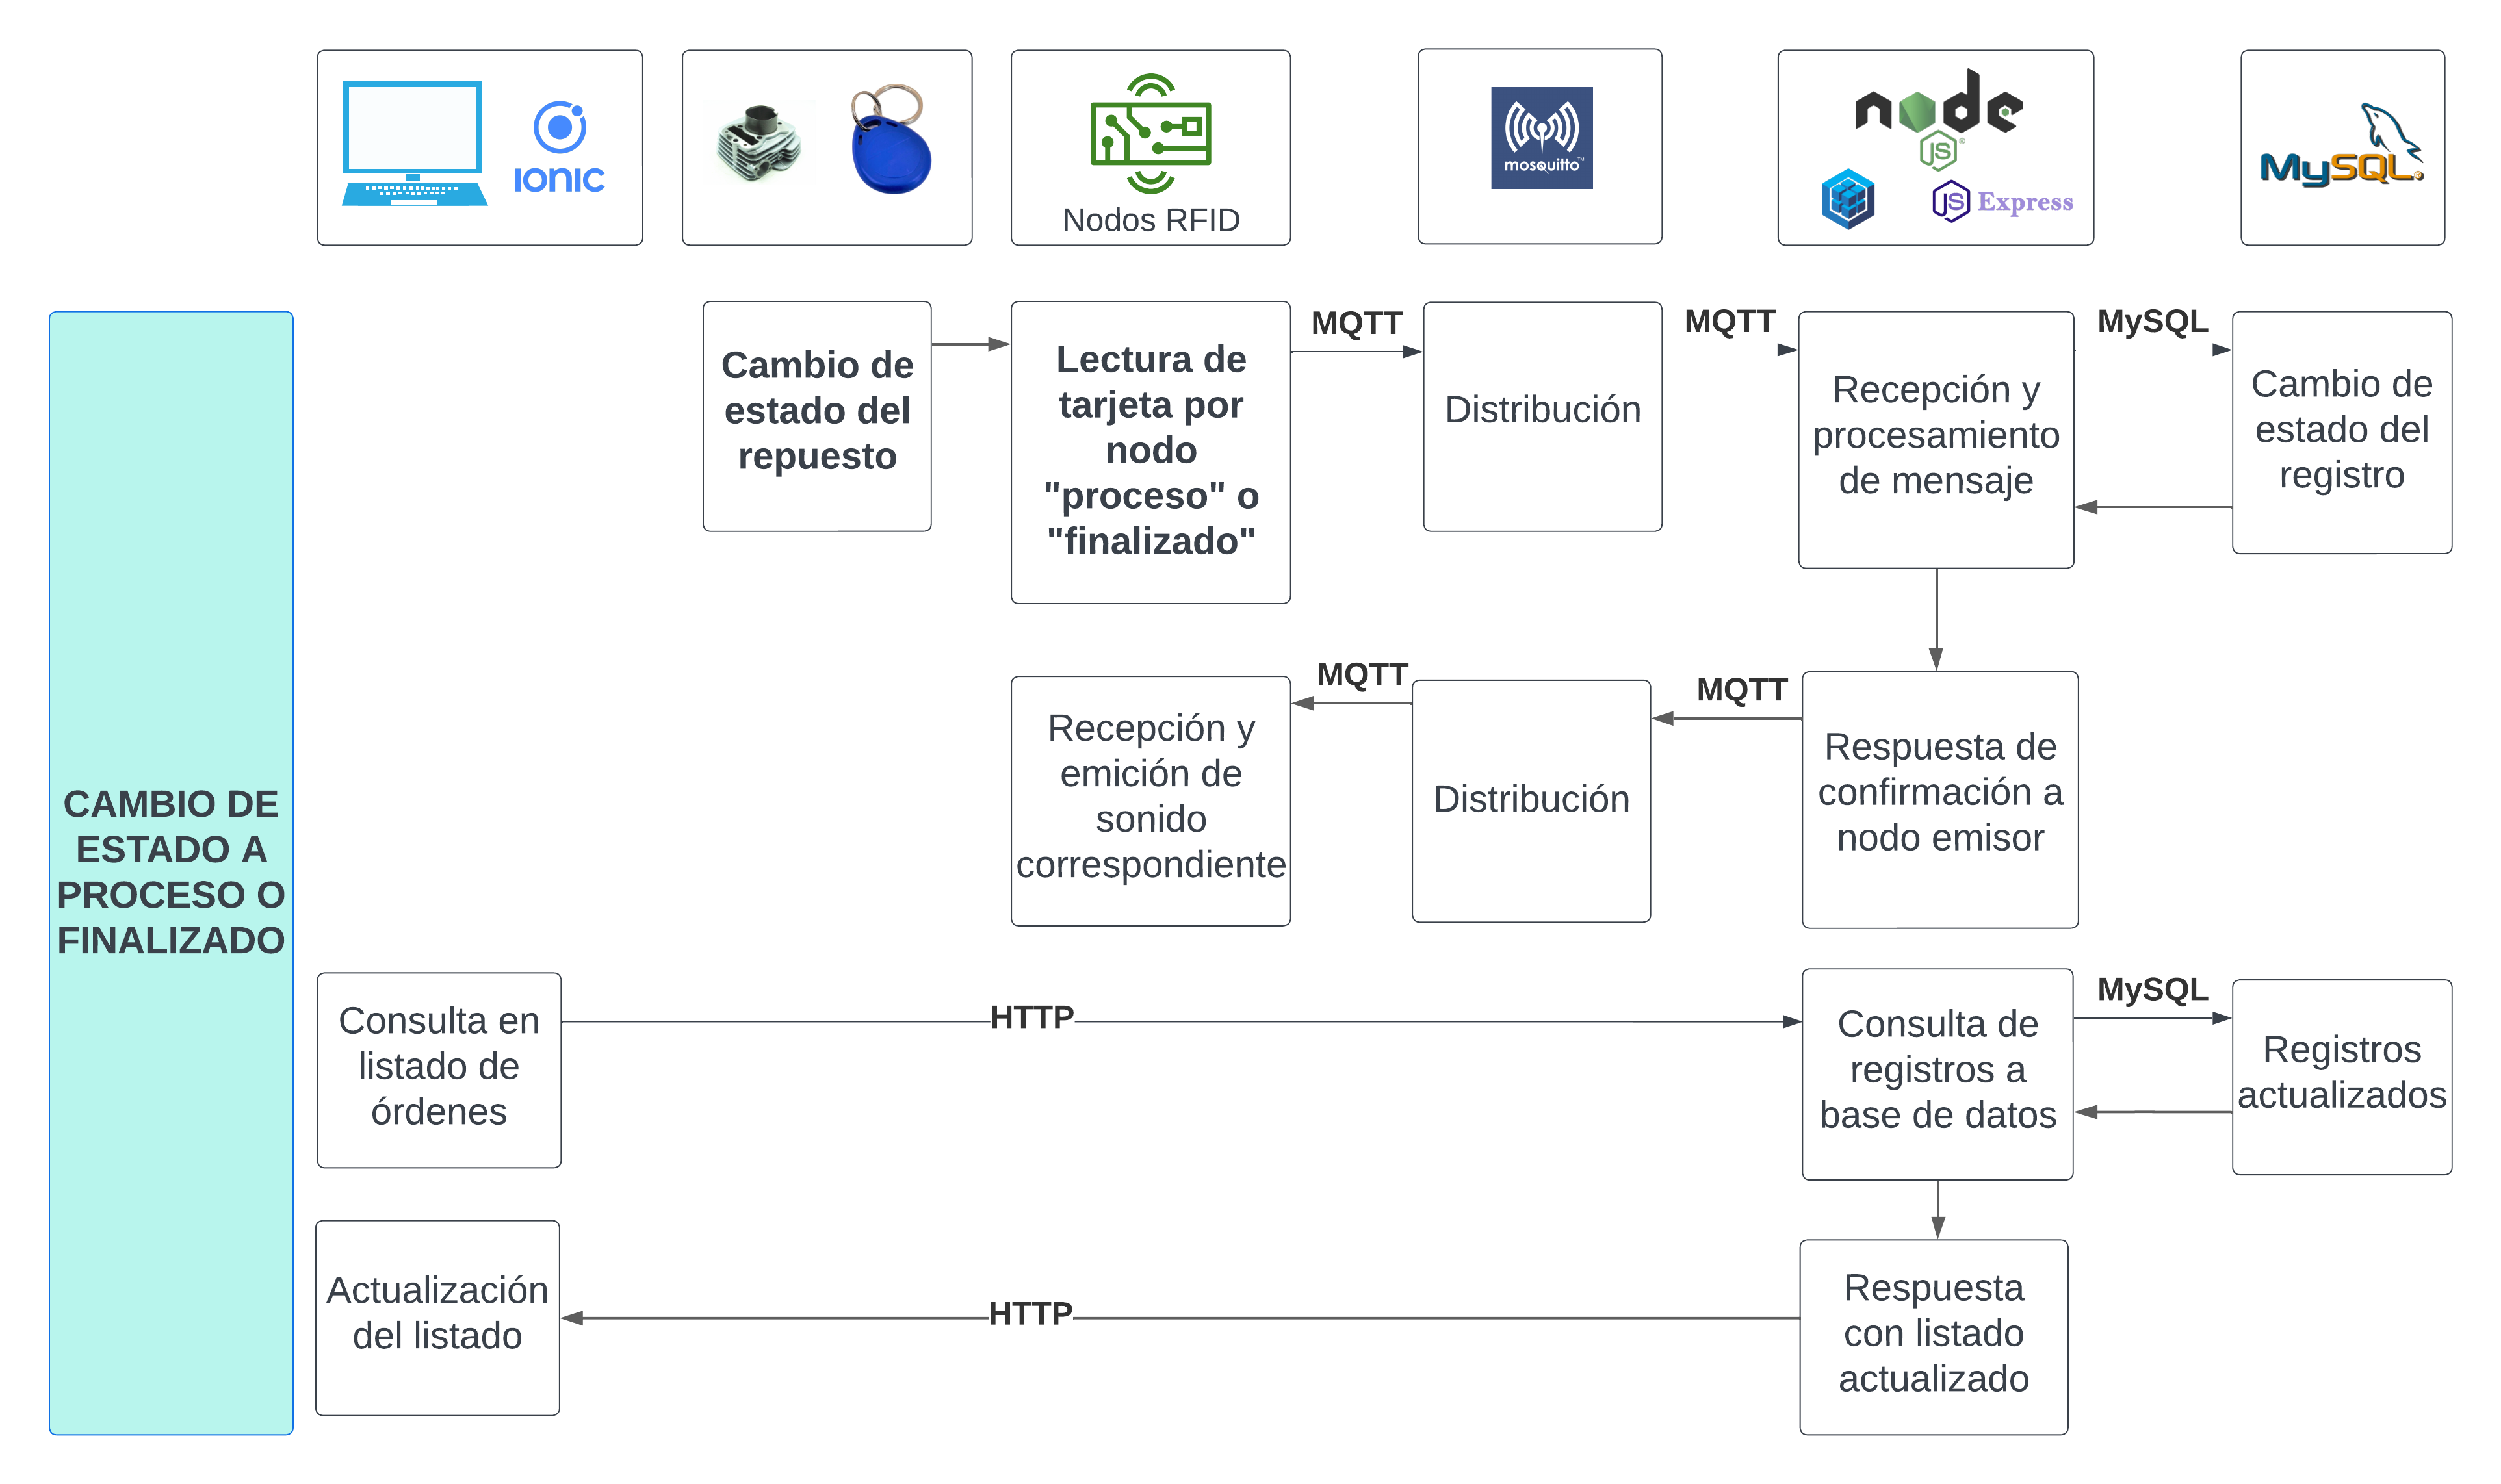
\includegraphics[width=\textwidth]{./Figures/flujo-cambio-estado.png}
	\caption{Flujo en el cambio de estado de una orden de trabajo.}
	\label{fig:flujocambioestado}
\end{figure}

El flujo inicia cuando un trabajador inicia o finaliza una orden, cambiando el estado de la misma a en proceso o finalizada. Para actualizar el estado de la orden debe pasar la tarjeta RFID asociada al repuesto por el nodo correspondiente, de esta manera se transmite la información por protocolo MQTT hasta la API de backend, esta última realiza el la actualización en la base de datos y responde al nodo por medio de MQTT informando si la operación tuvo éxito. El nodo emitirá un sonido que informará al usuario del resultado obtenido (tabla de sonidos en capítulo \ref{subsec:mqttnodos}). Al mismo tiempo el usuario de la aplicación web verá reflejada la actualización del estado de la orden correspondiente en el listado de ordenes, ya que se está constantemente consultando por actualizaciones a la API por medio del protocolo HTTP utilizando el patrón observador de IONIC (detallado en el capítulo \ref{subsec:frontinterfaces}).

\subsection{Retiro de repuesto}
\label{subsec:flujoretiro}

En la figura \ref{fig:flujoretiro} se puede observar el flujo completo en el retiro de un repuesto.

\begin{figure}[ht]
	\centering
	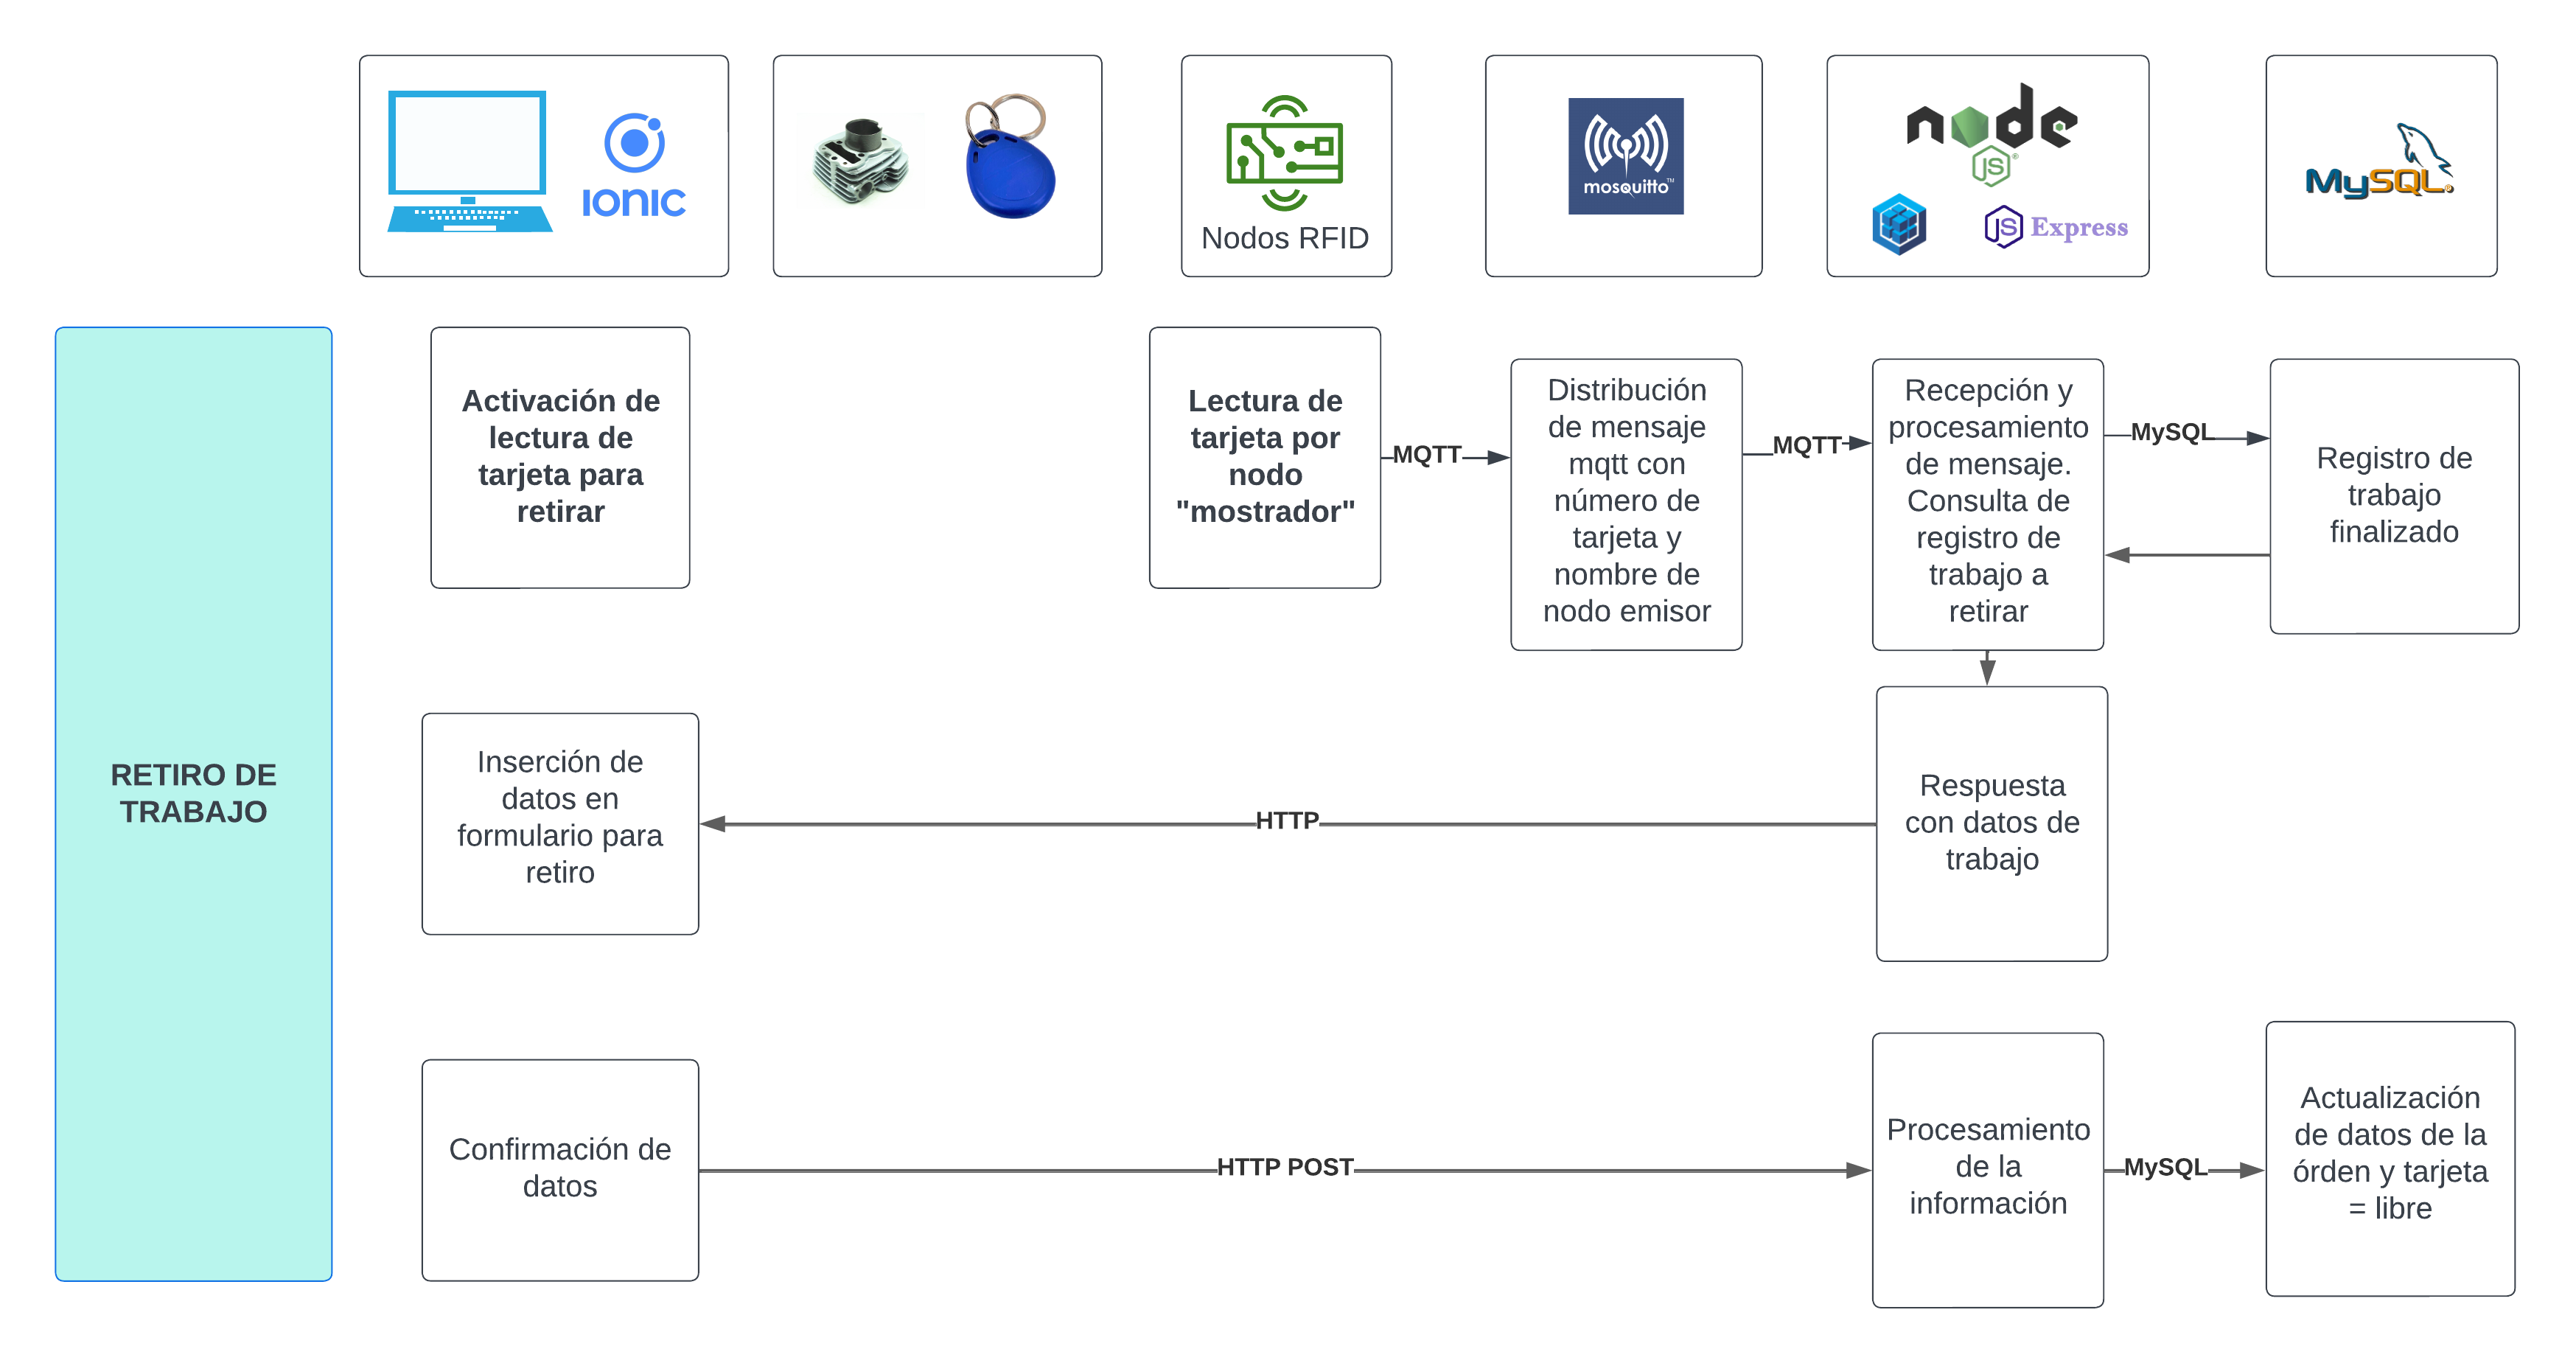
\includegraphics[width=\textwidth]{./Figures/flujo-retiro.png}
	\caption{Flujo en el retiro de una orden de trabajo.}
	\label{fig:flujoretiro}
\end{figure}

El flujo inicia cuando el usuario de la aplicación web realiza una activación de lectura de tarjeta en la pantalla de retiro. Esto ocasiona que la aplicación active un \textit{modo escucha} hacia la API, esperando a que el usuario pase la tarjeta asociada al repuesto por el nodo mostrador. Cuando esto sucede la API recibe por MQTT el número de tarjeta y mediante este recupera los datos de la orden correspondiente en la base de datos, luego devuelve los datos obtenidos a la aplicación web por medio del protocolo HTTP. La aplicación inserta todos estos datos en el formulario de retiro y, cuando el usuario confirma la operación, se realiza una petición HTTP con el método PUT para actualizar los datos de los registros. La tarjeta utilizada queda en estado \textit{libre} para ser reutilizada en una nueva orden de trabajo.

\section{Arquitectura de datos}
\label{sec:arquitecturadatos}
En la presente sección se desarrollará la arquitectura en la base de datos MySQL, el diseño y la implementación de las funciones con el ORM Sequelize.

\subsection{Diseño de base de datos}
\label{subsec:diagramabasededatos}

Se realizó un análisis de los requerimientos y los casos de usos o historias de usuario, a partir de esto se inició el diagrama con las tablas principales y sus relaciones, a medida que se avanzó en el desarrollo de la API y del sistema  se fueron añadiendo nuevas tablas y relaciones según las necesidades.

Se siguió el modelo entidad relación mencionado en el capítulo \ref{subsec:RDBMS} y en total se implementaron más de 15 tablas con sus respectivas relaciones. Se describe a continuación su implementación con el ORM Sequelize. 



\subsection{Estructura de archivos para ORM}
\label{subsec:estructuraorm}
Para el desarrollo de la base de datos se utilizó el ORM Sequelize. Como se menciona en el capítulo \ref{subsec:sequelize}, existen múltiples ventajas al utilizar un ORM en vez de directamente programar la base de datos en lenguaje SQL, se tuvieron en cuenta esas ventajas a la hora de optar por realizar el desarrollo con este ORM. 

La estructura de carpetas y archivos está definida previamente por el ORM y se pueden realizar personalizaciones según se necesite. 

En la figura \ref{fig:estructuraorm} se puede ver la estructura implementada.

\begin{figure}[h]
	\centering
	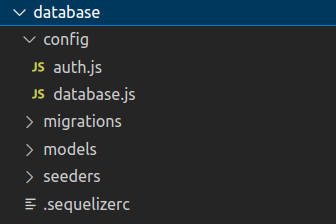
\includegraphics[scale=.50]{./Figures/estructuraorm.png}
	\caption{Estructura de carpetas y archivos para ORM Sequelize.}
	\label{fig:estructuraorm}
\end{figure}

Dentro de la carpeta \textit{config} se definen los archivos de configuración de Sequelize y el acceso a la base de datos MySQL.

En la carpeta \textit{migrations, models y seeders} se encuentran todos los archivos Javascript para las migraciones, los modelos y semillas, estos archivos se detallarán en las próximas secciones. 

El archivo \textit{.sequelizerc} sirve para definir la ubicación de los modelos, migraciones, semillas y otros archivos generados por Sequelize.


\subsection{Desarrollo de modelos y tablas}
\label{subsec:modelobasededatos}



A continuación se presentan algunos fragmentos de código fuente empleados para el desarrollo de la base de datos, siguiendo esta misma modalidad se realizaron todas las tablas de la base de datos, sus modificaciones y sus respectivas migraciones.


En el código \ref{cod:sequelizeclimodel} se ejecuta en la terminal de linux para crear el archivo para el modelo y el archivo para la migración de la tabla para ``orden de trabajo". En la línea se define el nombre del modelo y un atributo id. 

\begin{lstlisting}[label=cod:sequelizeclimodel,caption=Código CLI para crear modelo y migración en Sequelize.]
npx sequelize-cli model:generate --name mqtt_messages_gral --attributes id:integer
\end{lstlisting}

En el código \ref{cod:sequelizeclimodelcode} se muestra un ejemplo de definición para el modelo de una tabla.

\begin{lstlisting}[label=cod:sequelizeclimodelcode,caption= Código para un modelo en Sequelize.]
'use strict';
const {Model} = require('sequelize');
module.exports = (sequelize, DataTypes) => {
  class OrdenTrabajo extends Model {
    
    static associate(models) {
      //OrdenTrabajo.X pertenece a X
      OrdenTrabajo.belongsTo(models.Trabajo)
      
      //OrdenTrabajo tiene ids en la tabla Eventos_mqtt
      OrdenTrabajo.hasMany(models.Eventos_mqtt);

      })

      // Orden de trabajo tiene muchos Repuestos N:M
      OrdenTrabajo.belongsToMany(models.Repuesto, {
        through: 'Orden_Repuesto'
      })
    }
  }
  OrdenTrabajo.init({
    id: {
      allowNull: false,
      autoIncrement: true,
      primaryKey: true,
      type: DataTypes.INTEGER
    },
    precio:{
      type: DataTypes.INTEGER
    },
    entrega:{
      type: DataTypes.INTEGER
    },
    createdAt: {
      allowNull: false,
      type: DataTypes.DATE
    },
    updatedAt: {
      allowNull: false,
      type: DataTypes.DATE
    }
  }, {
    sequelize,
    modelName: 'OrdenTrabajo',
    tableName: 'OrdenTrabajo',
  });
  return OrdenTrabajo;
};

\end{lstlisting}

En las líneas 1 a la 4 se realizan las declaraciones de la biblioteca y el nombre del modelo, 
luego en las líneas 6 a la 19 se definen las relaciones que tendrá el modelo, los tipos de relaciones pueden ser 1 a 1, 1 a muchos o muchos a muchos. Luego a partir de la línea 21 se definen los campos de la tabla o modelo, se definen también los atributos de los campos y el tipo de datos. En las líneas 44 y 45 se define el nombre personalizado que tendrá la tabla en la base de datos y el nombre del modelo que reconocerá el ORM. Por último en la línea 47 se retorna la clase creada, de esta manera podrá ser utilizada en otras partes del código fuente.


\subsection{Desarrollo de migraciones}
\label{subsec:migracionesbasededatos}

Como se menciona en la sección anterior, el archivo con la estructura inicial de migraciones se crea a través del CLI de Sequelize al momento de crear el modelo para una tabla, luego hay que personalizar esta estructura para que quede igual al modelo definido previamente. 

A continuación, en el código \ref{cod:sequelizemigrationcore} se representa una parte del código \textit{javascript} para la migración del modelo ``orden de trabajo".

\begin{lstlisting}[label=cod:sequelizemigrationcore, caption= Código para migración en Sequelize.]
'use strict';
module.exports = {
  async up(queryInterface, Sequelize) {
    await queryInterface.createTable('OrdenTrabajo', {
      id: {
        allowNull: false,
        autoIncrement: true,
        primaryKey: true,
        type: Sequelize.INTEGER
      },
      precio:{
        type: Sequelize.INTEGER
      },
      entrega:{
        type: Sequelize.INTEGER
      },
      TrabajoId:{
        type: Sequelize.INTEGER,
        references:{model:'Trabajo', key:'id'}
      },
      createdAt: {
        allowNull: false,
        type: Sequelize.DATE
      },
      updatedAt: {
        allowNull: false,
        type: Sequelize.DATE
      }
    });
  },
  async down(queryInterface, Sequelize) {
    await queryInterface.dropTable('OrdenTrabajo');
  }
};
\end{lstlisting}

Como se puede notar, el código es muy parecido al del modelo, con la diferencia que en este caso, además de los campos y sus atributos, se deben definir también las claves que representan a las relaciones 1 a muchos que tendrá esta tabla, dejando de lado el resto de relaciones. 

Otra de las particularidades principales del archivo de migración es que contiene dos funciones que se ejecutan de manera asíncrona, la función up y down, la primera creará la tabla y la segunda se ejecuta en caso de alguna falla y elimina la tabla. 
  

\subsection{Interacción con la base de datos}
\label{subsec:interaccionbasededatos}

En Sequelize se pueden realizar todas las funciones necesarias para interactuar con la base de datos, ya sea para insertar, actualizar o eliminar registros, como así también los métodos para leer registros utilizando filtros o condiciones particulares.

A continuación se presentan a modo de ejemplo algunos fragmentos de código Javascript empleados para tal fin:

El código \ref{cod:getordenescode} se utiliza para traer todas las ordenes de trabajo existentes, incluyendo otros modelos relacionados a este.

\begin{lstlisting}[label=cod:getordenescode,caption= Código para traer datos en Sequelize.]
/**
 * 
 * @method getOrdenesTrabajo 
 * @description
 * Traer todas las ordenes de trabajo existentes
 * @returns
 * listado de todas las ordenes de trabajos existentes
 */
const getOrdenesTrabajo = async (req, res)=>{
    const ordenesTrabajo = await OrdenTrabajo.findAll({
        include:[
            {model:Cliente},
            {model: Estado},
            {model: Moto},
            {model: Trabajo},
            {model: Usuario},
        ]
    });
    return res.json(ordenesTrabajo)
}
\end{lstlisting}

En código \ref{cod:nuevoregistro} representa de manera resumida cómo crear un nuevo registro, se quitaron algunas partes del código que son relevantes a esta sección:

\begin{lstlisting}[label=cod:nuevoregistro,caption=Código para crear nuevo registro en la base de datos.]
/**
 * Crear nueva orden de trabajo
 */
const nuevaOrdenTrabajo = async (req,res) => {
        const nuevaOrdenTrabajo = await OrdenTrabajo.create(
            req.body, 
            );
        return res.json(nuevaOrdenTrabajo);     
    } catch (error) {
        return res.status(400).json({
            error:error.message, 
            message:'Error cargando orden',
            context: 'api > controllers > ordenTrabajoController > nuevaOrdenTrabajo'
        })  
\end{lstlisting}

En las líneas 5 y 6 es dónde se realiza la creación del registro, pasando los datos que se reciben como parámetros en el \textit{body} de la petición HTTP.

Por último, en el código \ref{cod:updateregistro} se muestra cómo actualizar un registro de la base de datos, previamente trayendo el objeto por su ID:

\begin{lstlisting}[label=cod:updateregistro,caption=Código resumido para actualizar un registro en la base de datos.]
// Traigo la Orden de trabajo
let orden = await OrdenTrabajo.findOne({
            where: {
                id:req.params.id_orden,
                }
            });
            
// Modifico estado, precio, detalle y entrega de la Orden
        await orden.update(
            {
                EstadoId : estado.id,
                precio: req.body.precio,
                entrega: req.body.entrega,
                detalle: req.body.detalle
            });
\end{lstlisting}

Se puede observar que en la línea 3 se busca el registro mediante su ID y se guarda el mismo en una variable, luego se utiliza esa variable para realizar la actualización de los datos, por lo que esa variable pasa a ser un ``objeto de Sequelize" que puede ser tratado directamente como entidad única de la base de datos, facilitando su uso mediante el ORM.


\section{Desarrollo API REST}
\label{sec:arquitecturaapirest}

La lógica del backend se centra principalmente en la API REST desarrollada, en la misma se utilizaron diferentes tecnologías las cuales están descritas en el capítulo \ref{sec:backend}.

A continuación se detalla su desarrollo e implementación.

\subsection{Patrón de desarrollo}
\label{subsec:apipatron}

Se implementó una arquitectura de software orientada a eventos, nativa de Node.js, y la organización modular del código también llamado \textit{``event-driven"}.

En la organización modular se estructura el código de la aplicación en pequeñas piezas reutilizables. Esto hace que el código sea más fácil de mantener y actualizar a medida que la aplicación crece y evoluciona.

En la figura \ref{fig:apiestructura} se presenta la estructura de carpetas utilizada siguiendo el modelo mencionado. 

\begin{figure}[ht]
	\centering
	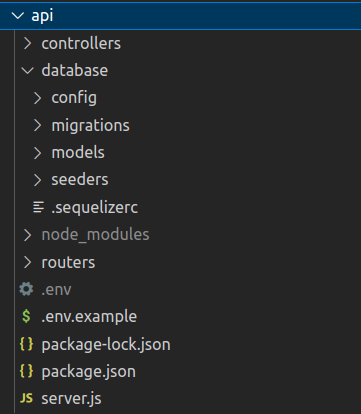
\includegraphics[scale=.50]{./Figures/api-estructura-archivos.png}
	\caption{Estructura de carpetas en patrón de desarrollo modular.}
	\label{fig:apiestructura}
\end{figure}

Dentro de cada una de las carpetas se encuentran los archivos Javascript correspondientes. El archivo \textit{server.js} es el punto de partida de la API y donde se realizan las configuraciones de conexión a bases de datos con Sequelize, configuración de Express, se definen los puertos a utilizar, la conexión MQTT, se declaran las rutas o \textit{routes}, entre otras configuraciones.

En el archivo \textit{package.json} se encuentran configuraciones y datos fundamentales para la aplicación, entre estas están: el nombre de la aplicación, la versión, descripción del proyecto, los scripts de inicio y ejecución, las dependencias del proyecto, bibliotecas y paquetes de terceros utilizados, las versiones específicas de las dependencias requeridas y la información de licencia. En este archivo se define, por ejemplo, el uso de Sequelize y Express y sus respectivas versiones.

El archivo .env es un archivo que no se versiona, esto significa que no se resguarda el historial de cambios del archivo, esto se debe a que contiene información sensible que debe mantenerse segura y no debe versionarse ni subirse a internet. En cada entorno dónde la aplicación sea instalada se deberá crear este archivo manualmente y escribir las definiciones de manera manual. Se declara, por ejemplo, usuario y contraseña para la conexión a base de datos, credenciales para conexión a \textit{broker} MQTT, direcciones IP o URL, conexión a Wi-Fi, entre otros datos sensibles.

En las siguientes secciones se detallan las carpetas \textit{routers} y \textit{controllers}.

\subsection{Ruteo de la API}
\label{subsec:apirouters}

En la carpeta \textit{routers} se encuentran los archivos Javascript que corresponden a las rutas que maneja Express para recibir las peticiones o \textit{requests} HTTP provenientes desde fuera de la API, generalmente desde el cliente frontend.

En la figura \ref{fig:apiroutes} se muestran los archivos de ruteo que se crearon siguiendo el patrón modular, separando las rutas según su entidad o funcionalidad.

\begin{figure}[ht]
	\centering
	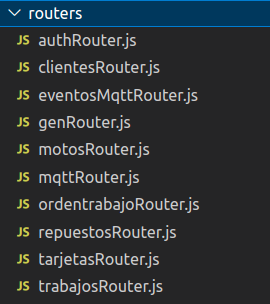
\includegraphics[scale=.50]{./Figures/api-routes.png}
	\caption{Estructura de archivos en carpeta de rutas.}
	\label{fig:apiroutes}
\end{figure}

En el archivo \textit{ordentrabajoRouter.js} se manejan las peticiones a rutas referentes a las ordenes de trabajo, de la misma manera para los demás archivos. 

En el código \ref{cod:routesot} se presenta un fragmento de ruteo correspondiente a ordenes de trabajo:


\begin{lstlisting}[label=cod:routesot,caption=Código de ruteo para ordenes de trabajo.]
    /**
     * Nueva orden de trabajo
     * @params data, estado = espera
     * Recibe datos para la orden de trabajo
     * incluido el numero de tarjeta rfid
     */
    ordentrabajoRouter.post('/nueva',
        ordentrabajoCtrl.nuevaOrdenTrabajo);
\end{lstlisting}

En la declaración de esta ruta se puede observar que la dirección de la ruta en cuestión es \textit{/nueva} y se define con el método \textit{post()} en un objeto de \textit{router} llamado \textit{ordentrabajoRouter}. Este método indica que la ruta es accesible mediante una solicitud HTTP POST, que es utilizada para enviar información a un servidor para crear un recurso.

Además, se especifica un controlador de ruta \textit{(handler)}. El controlador es una función que se ejecuta cuando se realiza una solicitud HTTP a la ruta especificada. En este caso, el controlador de ruta se llama \textit{nuevaOrdenTrabajo} y se define en el archivo \textit{ordentrabajoCtrl}, más adelante se detallará la carpeta \textit{controllers} y sus características.

Cuando se realiza una solicitud HTTP POST a la ruta \textit{/nueva}, Express ejecutará automáticamente la función \textit{nuevaOrdenTrabajo} definida en el controlador de ruta \textit{ordentrabajoCtrl}.

De esta manera se logra separar la lógica de ruteo de la lógica de procesos y acceso a datos, siguiendo el patrón modular mencionado previamente.

\subsection{Controladores de la API}
\label{subsec:apicontrollers}

Como se mencionó en la sección previa, los controladores son funciones que se ejecutan luego de resolver la ruta a la cual están asociados. 

En la figura \ref{fig:apicontrollers} se puede ver como en la carpeta \textit{controllers} se definieron los controladores siguiendo el patrón modular de desarrollo, teniendo en cuenta la entidad o la funcionalidad que se desea procesar.

\begin{figure}[ht]
	\centering
	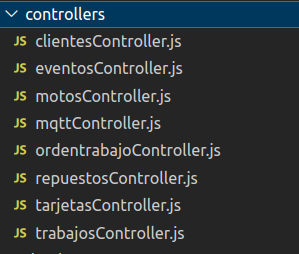
\includegraphics[scale=.50]{./Figures/api-controllers.png}
	\caption{Estructura de archivos en la carpeta \textit{controllers}.}
	\label{fig:apicontrollers}
	
\end{figure}

En el código \ref{cod:controllerlist} se observa un fragmento de código del controlador para obtener un listado de todas las motos de la base de datos:

\begin{lstlisting}[label=cod:controllerlist,caption=Código de controlador para obtener listado de motos.]
const {Moto} = require('../database/models/index');

const { Op, Sequelize } = require("sequelize");
const { response } = require('express');

//controller
const listarMoto = async (req, res)=>{
    try {
        const listadoMotos = await Moto.findAll({});
        
        return res.status(200).json({
            listadoMotos
        }); 

    } catch (error) {
        return res.status(400).json({
            error: error.message,
            message: 'Error listando motos'
        })
    }
    
};
\end{lstlisting}

La primera línea del código importa el modelo \textit{Moto} desde el archivo principal para los modelos de Sequelize \textit{index.js} ubicado en la carpeta \textit{models}. En la segunda línea, se importan las funciones \textit{Op y Sequelize} desde la librería Sequelize, estas funciones se utilizan para realizar operaciones y consultas en la base de datos. Luego, se define el controlador \textit{listarMoto} que se encarga de listar todas las motos de la base de datos. Dentro del controlador, se utiliza el método \textit{findAll()} de Sequelize para buscar todos los registros. Si la consulta a la base de datos se realiza con éxito, se devuelve un objeto \textit{JSON} con el listado de motos y un código de estado HTTP 200. En caso de que la consulta falle, se devuelve un objeto \textit{JSON} con el mensaje de error y un código de estado HTTP 400.

Finalmente, se exporta el controlador \textit{listarMoto} para que pueda ser utilizado en otras partes de la aplicación.

De manera similar se desarrollaron todos los controladores para las diferentes rutas de la aplicación. 

\subsection{Endpoints HTTP}
\label{subsec:apiendpointshttp}

Para la organización del desarrollo se realizó una tabla con todos los datos necesarios para los \textit{endpoints} o rutas de la API. 

En la tabla \ref{tabla:endpointshttp} se puede observar algunas de las rutas HTTP correspondientes a las ordenes de trabajo.

\begin{table}[H]
\centering
\begin{tabular}{|*{4}{>{\centering\arraybackslash}p{3cm}|}}
\hline
Método & URL & Función & Detalle\\
\hline
GET & /todos & Obtener ordenes de trabajo.  & ...  \\
\hline
GET & /filtrado & Filtrado por campo. & Endpoint para traer ordenes según filtro: fecha, estado, etc. \\
\hline
GET & /cliente & Filtrado orden de trabajo por DNI del cliente. & Para la pantalla búsqueda orden de trabajo del cliente. \\
\hline
POST & /nueva & Insertar nueva orden. & Datos de la orden con número de tarjeta incluida.  \\
\hline
PUT & /cambiarestado & Cambiar estado de orden y tarjeta. & Para proceso o finalizado de orden de trabajo.  \\
\hline
\end{tabular}
\caption{Endpoints HTTP}
\label{tabla:endpointshttp}
\end{table}


A medida que se avanzó en el desarrollo se fueron marcando en verde las filas de las rutas finalizadas, además se fue agregando más detalles o parámetros según requerimientos o necesidades.

\section{Comunicación MQTT}
\label{sec:mqttarquitectura}


\subsection{Diagrama MQTT}
\label{subsec:mqttdiagrama}

\begin{figure}[ht]
	\centering
	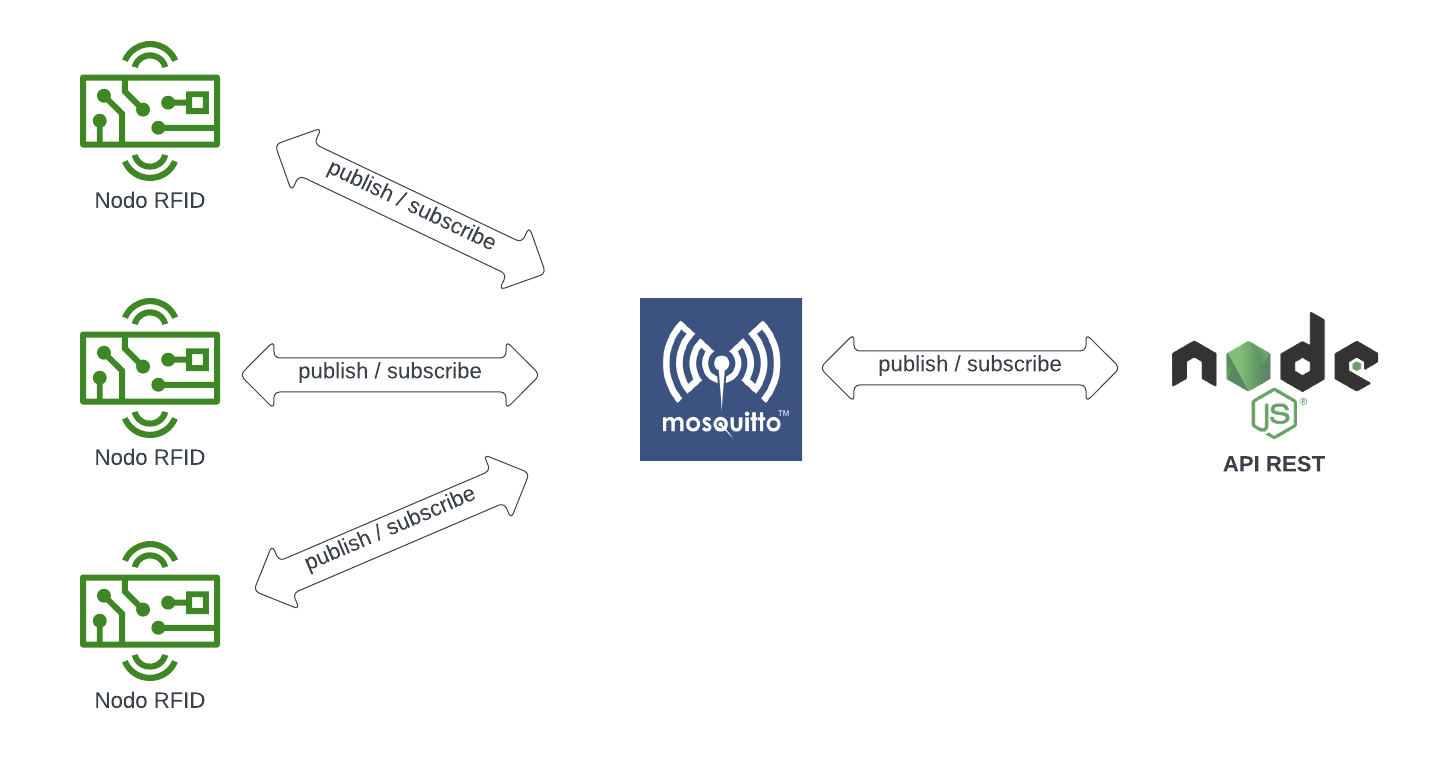
\includegraphics[scale=.15]{./Figures/mqtt-funciones.png}
	\caption{Diagrama de funciones MQTT.}
	\label{fig:mqttfunciones}
	
\end{figure}

En la figura \ref{fig:mqttfunciones} se pueden apreciar los distintos actores que intervienen en la comunicación MQTT del sistema. Los nodos RFID representan a cada ESP32 con el módulo lector RC522 mencionados en el capítulo \ref{subsec:esp32}, estos se encargan de marcar el estado específico de una orden de trabajo. En el centro se ubica el \textit{broker} Mosquitto el cual se encarga de la distribución de los mensajes a los demás módulos y a la derecha está la API REST desarrollada en Node.js la cual recibe los mensajes provenientes de los nodos y realiza el proceso correspondiente, además de enviar publicaciones a modo de información y para \textit{logs}.

\subsection{Topics MQTT}
\label{subsec:mqtttopics}

Al igual que con las rutas HTTP, se organizan los \textit{topics} MQTT en una tabla según el nodo o sensor.

La lista completa de \textit{topics} implementados es la siguiente:
\begin{itemize}
\item *: API backend se suscribe a todos los mensajes.
\item nodo/discriminar: emite nodo ``mostrador`` para ingresar o retirar ordenes de trabajo. Recibe API backend.
\item nodo/cambiarestado: emite nodo ``proceso`` o ``finalizado`` para cambiar el estado de una orden de trabajo. Recibe API backend.
\item api/error/mostrador: emite la API de backend para informar un error en el proceso. Recibe nodo ``mostrador``.
\item api/error/proceso: emite la API de backend para informar un error en el proceso. Recibe nodo ``proceso``.
\item api/error/finalizado: emite la API de backend para informar un error en el proceso. Recibe nodo ``finalizado```.
\item api/confirmacion/mostrador: emite la API de backend para informar proceso exitoso. Recibe nodo ``mostrador``.
\item api/confirmacion/proceso: emite la API de backend para informar proceso exitoso. Recibe nodo ``proceso``.
\item api/confirmacion/finalizado: emite la API de backend para informar proceso exitoso. Recibe nodo ``finalizado``.

\end{itemize}

\subsection{Broker MQTT}
\label{subsec:mqttbroker}

Para la implementación en el servidor del sistema en la Raspberry Pi del \textit{broker} MQTT ``Eclipse Mosquitto" se utilizó un servicio de Docker Compose el cual permite levantar el \textit{broker} y sus configuraciones.

En la figura \ref{fig:mqttestructuracarpetas} se puede observar la estructura de carpetas y archivos que se implementa en el contenedor de Docker para este servicio. 

\begin{figure}[H]
	\centering
	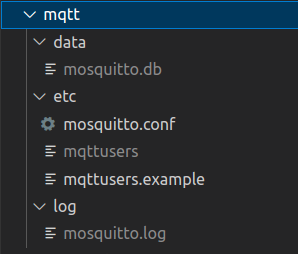
\includegraphics[scale=.60]{./Figures/mqtt-estructura-carpetas.png}
	\caption{Estructura de carpetas del servicio Eclipse Mosquitto en Docker.}
	\label{fig:mqttestructuracarpetas}
\end{figure}

A continuación se listan los detalles de cada carpeta:

\begin{itemize}
	\item En la carpeta \textit{data} se encuentra el archivo de base de datos \textit{mosquitto.db} donde se pueden persistir los mensajes MQTT según la configuración de persistencia implementada.
	\item En la carpeta \textit{etc} se encuentra el archivo de configuración principal del \textit{broker}: \textit{mosquitto.conf}, aquí se declaran todos los parámetros con los cuales Docker Compose levantará el servicio. El archivo \textit{mqttusers} persiste de manera encriptada las credenciales de acceso para los clientes MQTT, estos usuarios son administrados por línea de comando en la terminal \textit{bash} ingresando al contenedor específico. Por último se agregó un archivo con el ejemplo de comandos para administrar usuarios: \textit{mqttusers.example}.
	\item La carpeta \textit{log} contiene el archivo \textit{mosquitto.log} donde se registran todos los logs del servicio y que sirven para hacer un \textit{debug} o \textit{test} del mismo.	
\end{itemize}


\subsection{MQTT en nodos}
\label{subsec:mqttnodos}
Para implementar las comunicaciones MQTT en los nodos ESP32 se utilizó la biblioteca de código abierto PubSubClient \citep{WEBSITE:pubsubclient} que permite conexiones con servidores MQTT, publicar mensajes y suscribirse a los mensajes recibidos.

Como se describió en el capítulo \ref{Chapter1} cada nodo representa uno o más estados específicos en la cadena de procesos que se realizan en la empresa. Estos estados son declarados en el código fuente del microcontrolador ESP32, específicamente en un archivo de entorno, de manera que pueda ser modificado fácilmente en caso de ser necesario.

A continuación se describen los nodos y sus estados utilizados:

\begin{itemize}
\item Nodo 1, ``mostrador``: este nodo cumple la función de comunicar a la API REST por medio de MQTT el número de tarjeta que ha sido leída en el mostrador de atención a clientes de la empresa. De esta manera la API REST se encargará de asignar los estados ``espera`` o ``retirado`` a las ordenes de trabajo según corresponda.

\item Nodo 2, ``proceso``: este nodo se encarga de comunicar a la API REST que debe cambiar el estado de la orden de trabajo a ``proceso``, la API REST reconoce que el mensaje proviene de este nodo por el ``topic`` por lo que se envía el mensaje, y consulta a la base de datos qué orden de trabajo tiene el número de tarjeta recibida para ejecutar la actualización.

\item Nodo 3, ``finalizado``: de la misma manera que en el nodo 2, en este sensor se informa a la API REST que debe cambiar el estado de la orden de trabajo asociada a la tarjeta leída a ``finalizado``.
\end{itemize}

De esta manera el ciclo de lecturas de los nodos para una orden de trabajo es el siguiente: 

\begin{enumerate}
\item Nodo ``mostrador``, se asigna el estado ``espera``.
\item Nodo ``proceso``, se asigna el estado ``proceso``.
\item Nodo ``finalizado``, se asigna el estado ``finalizado``.
\item Nodo ``mostrador``, se asigna el estado ``retirado``.
\end{enumerate}

Cuando un nodo envía o recibe una señal MQTT emite alertas sonoras para informar al usuario si la operación correspondiente tuvo éxito o fracaso. En la figura \ref{fig:mqttsonidosnodos} se puede observar cómo se implementaron estas señales sonoras en los nodos. Además se puede ver que existen dos opciones de sonidos, una es en forma de una sola nota denominada en la tabla ``Sonidos Clásicos`` y otra es en forma de una melodía denominada ``Melodías``. Se configura en cada nodo la opción deseada desde las variables de entorno. Además se realiza en el código una validación para asegurarse que el tipo de \textit{buzzer} instalado es compatible con la opción ``Melodía``, en caso que no lo sea se ejecuta por defecto la opción ``Sonidos Clásicos``

\begin{figure}[H]
	\centering
	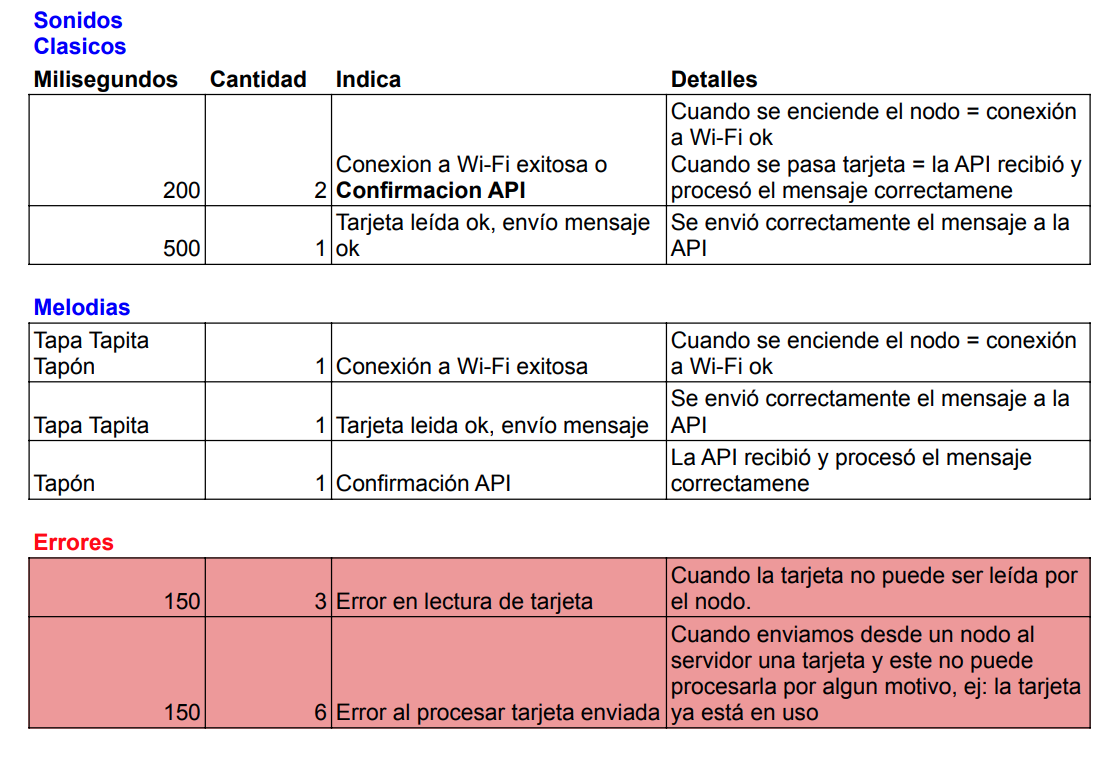
\includegraphics[width=\textwidth]{./Figures/nodos-beeps.png}
	\caption{Tabla de detalles de sonidos de nodos.}
	\label{fig:mqttsonidosnodos}
\end{figure}



\subsection{MQTT en API REST}
\label{subsec:mqttapi}

Se definió en la estructura de la API REST, descrita en el capítulo \ref{subsec:apipatron}, una sola ruta de entrada en el archivo principal de configuración \textit{server.js}, dónde se realiza la conexión al \textit{broker} MQTT y se subscribe a todos los \textit{topics} utilizando para ello el símbolo \#. 

Configuración y conexión a \textit{broker} MQTT:
\begin{lstlisting}[label=cod:mqttapiconect,caption= Configuración y conexión a \textit{broker} MQTT en API REST.]
 // mqtt config
    const mqtt = require('mqtt')
    const host = process.env.MQTT_SERVER
    const port = process.env.MQTT_PORT
    const clientId = `api_mqtt_${Math.random().toString(16).slice(3)}`
    
    // mqtt connect function
    const connectUrl = `mqtt://${host}:${port}`
    const mqtt_client = mqtt.connect(connectUrl, {
      clientId,
      clean: true,
      connectTimeout: 4000,
      username: process.env.MQTT_USER,
      password: process.env.MQTT_PASSWORD,
      reconnectPeriod: 3000,
    })
\end{lstlisting}

Como se puede observar en el código \ref{cod:mqttapiconect} se traen la mayoría de los parámetros desde las variables de entorno, esto se realiza para mantener un código limpio y que sea fácil de mantener, en caso de requerir algún cambio se realiza directamente en el archivo de variables de entorno evitando tener que cambiar en varias partes del código.

Primero se importa la librería MQTT y se definen las variables correspondientes al \textit{host} y puerto del \textit{broker}, así como un \textit{clientId} generado aleatoriamente. Luego se define la función de conexión al \textit{broker}, utilizando la URL compuesta por el \textit{host} y \textit{puerto} definidos anteriormente, y se especifican las opciones de conexión, incluyendo el \textit{clientId} generado, la limpieza de sesión en la conexión, un tiempo de espera de conexión de 4 segundos, el nombre de usuario y contraseña para la conexión y un período de reconexión de 3 segundos.


Subscripción a todos los \textit{topics}:

\begin{lstlisting}[label=cod:mqttapisub,caption=Subscripción a \textit{topics} en API REST.]
// subscribe to topics
    const topic = process.env.MQTT_TOPIC_ALL;
    mqtt_client.on('connect', () => {
      console.log('mqtt client Connected')
      mqtt_client.subscribe([topic], () => {
        console.log(`API Subscribe to topic '${topic}'`)
      })
    })
\end{lstlisting}

En el código \ref{cod:mqttapisub}, en la línea 2 se trae desde las variables de entorno el \textit{topic} correspondiente. Luego se inicia la conexión con el método \textit{on} y se realiza la suscripción con el método \textit{subscribe}. 

Luego los mensajes se rutean a un controlador MQTT que procesa todos los mensajes y siguiendo un flujo condicional realiza las acciones correspondientes.

A continuación se presenta un diagrama del flujo del código fuente para resolver los procesos según el mensaje MQTT recibido:

\begin{figure}[H]
	\centering
	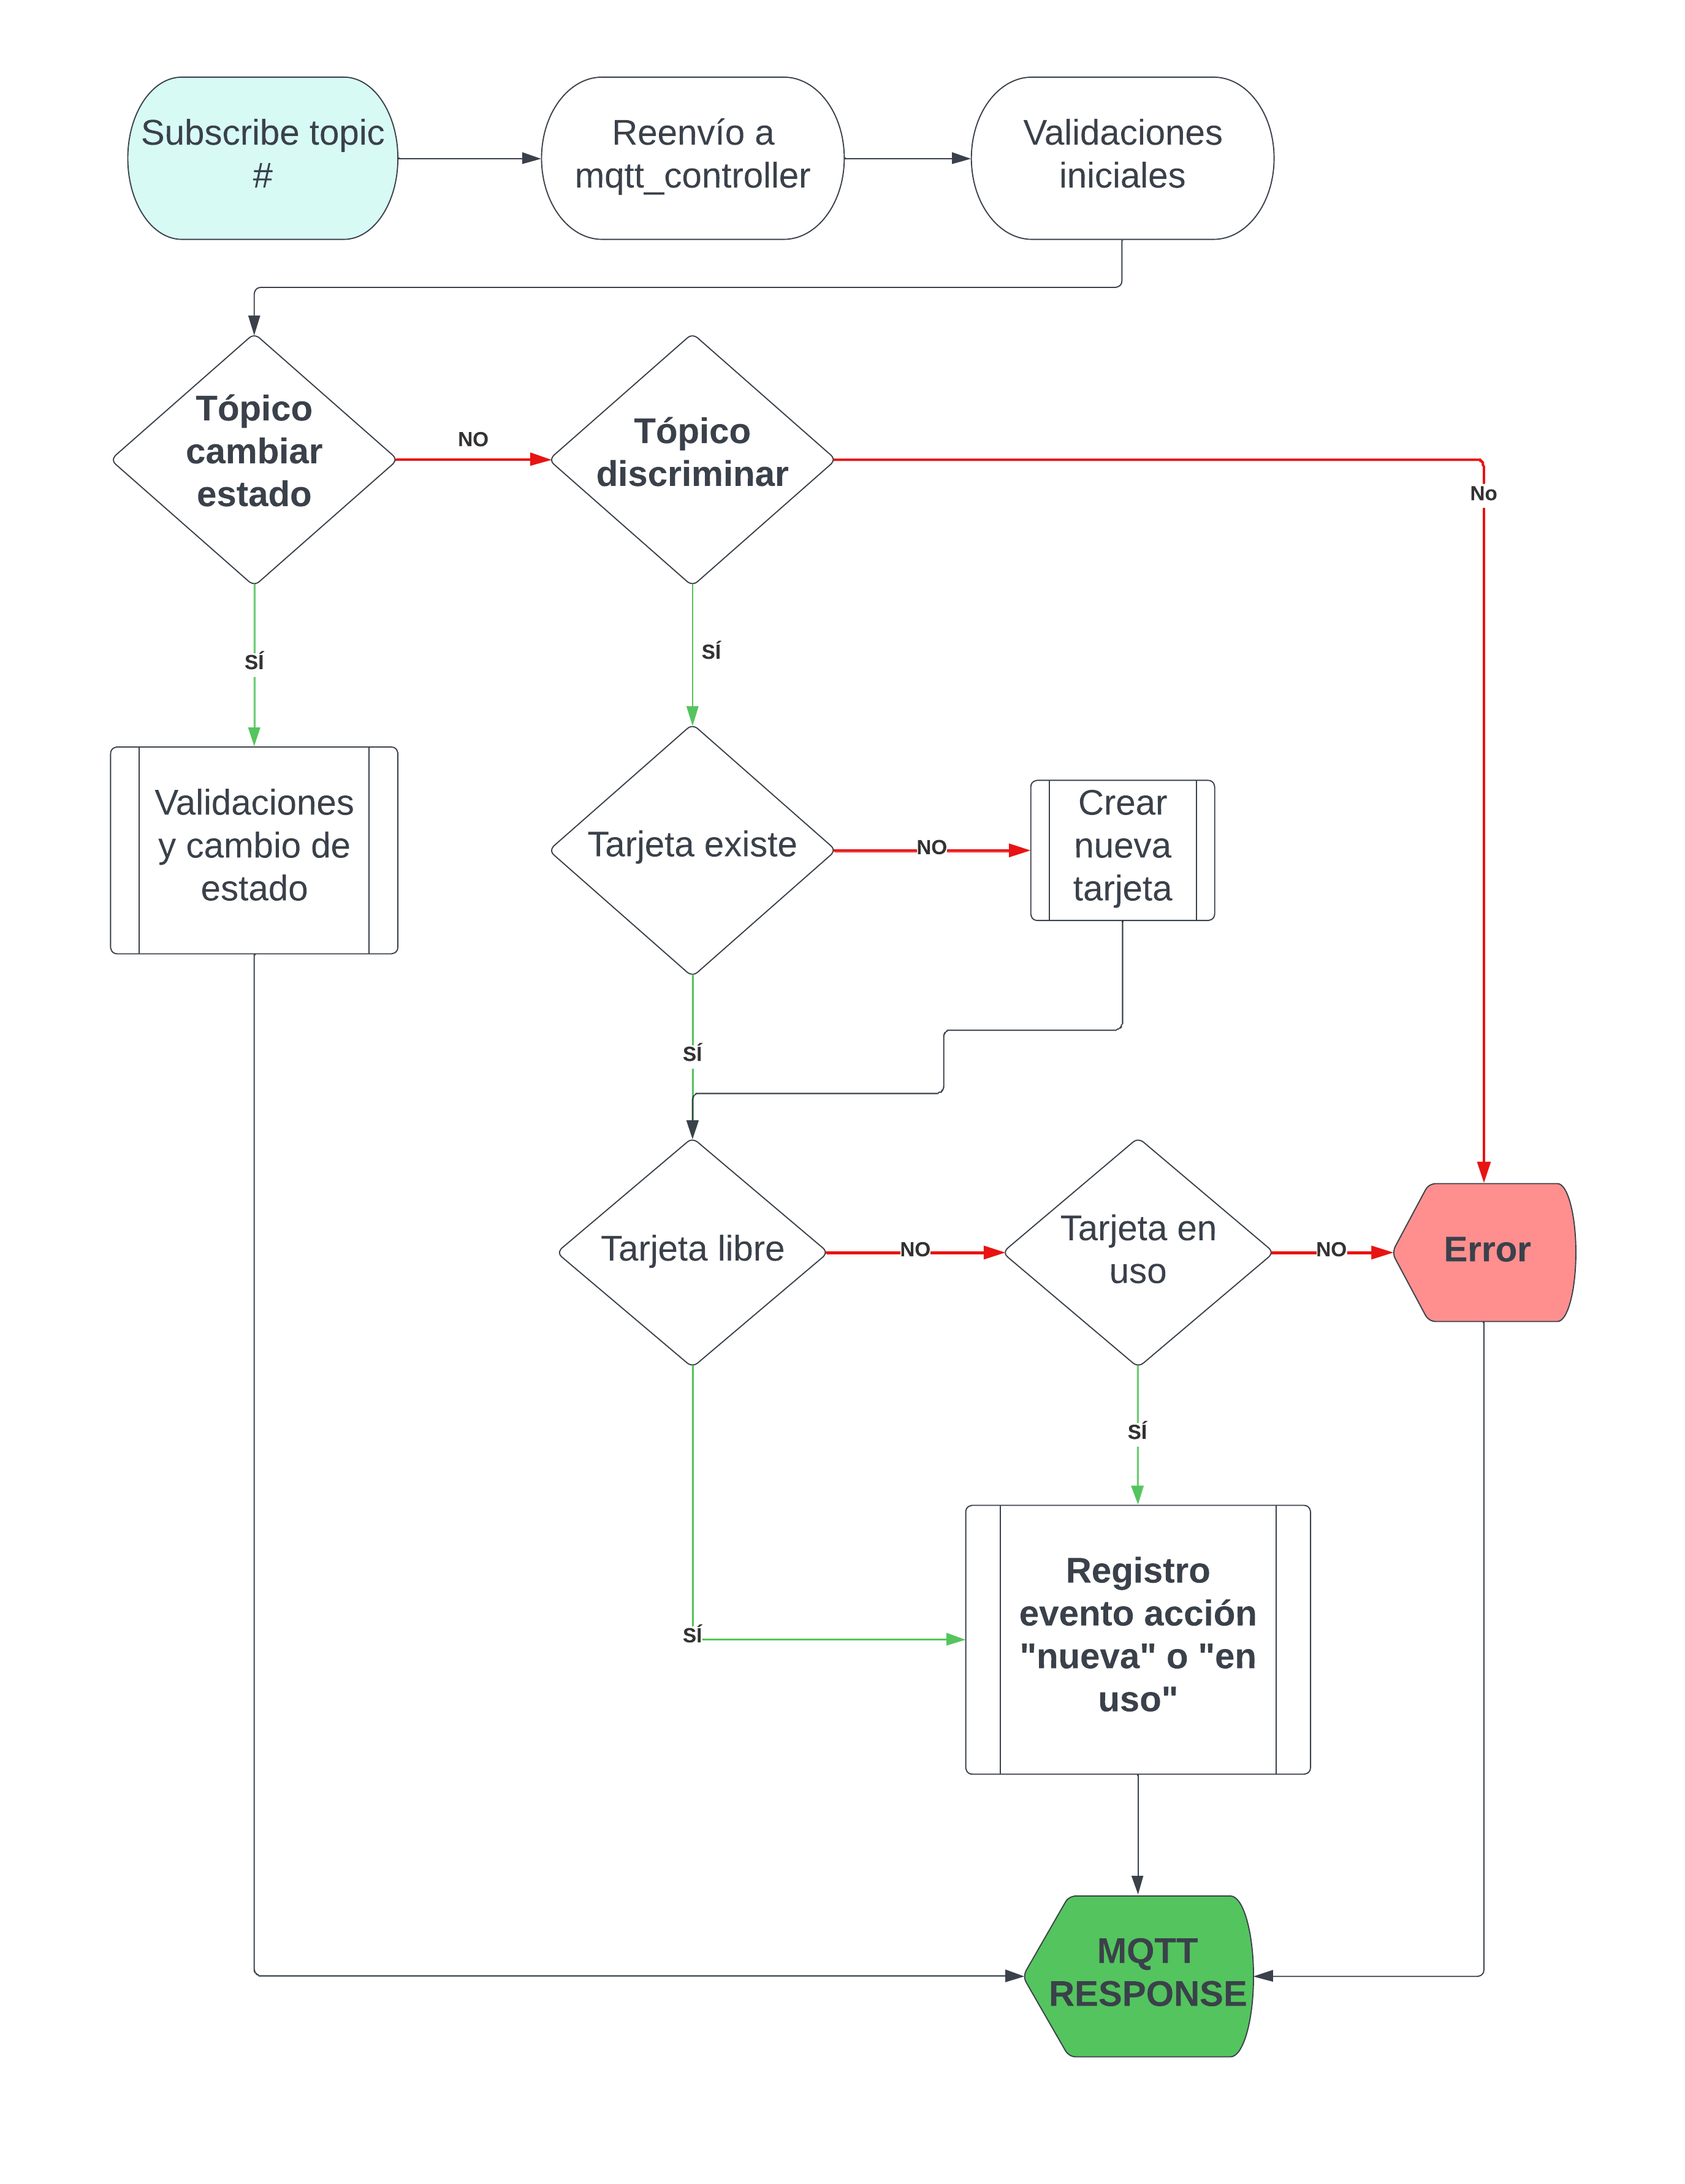
\includegraphics[width=\textwidth]{./Figures/mqtt-controller-api-2.png}
	\caption{Flujo de código fuente para MQTT en API REST.}
	\label{fig:mqttcontrollerapi}
\end{figure}

Como puede observarse en la figura \ref{fig:mqttcontrollerapi} las validaciones dependen tanto del \textit{topic} recibido como del estado de la tarjeta. De acuerdo a esto se realizan los procesos correspondientes y se devuelve un mensaje MQTT al nodo emisor el que, de acuerdo al mensaje recibido, emitirá una señal sonora a través del \textit{buzzer} para informar al usuario si la acción tuvo éxito o no. También se puede notar que una tarjeta RFID no necesita ser creada previamente para ser utilizada, ya que se realiza la validación correspondiente para crearla durante el mismo proceso en que se ingresa una nueva orden de trabajo.


\section{API para mensajería}
\label{sec:apimessenger}

Para el envío de mensajes por la aplicación WhatsApp \cite{whatsapp} se utilizó una API adicional \cite{api-whatsapp-ts} la cual fue personalizada para las necesidades de este sistema.

En esta sección se detalla cómo se implementó una API de mensajería para WhatsApp.

Esta API permite al usuario de la aplicación conectarse a WhatsApp con su teléfono móvil y enviar mensajes desde la aplicación a los clientes de manera automática.

\subsection{Implementación}
\label{subsec:apimessengerimplementación}

Para implementar está API se creó un contenedor en Docker de manera tal de separar este servicio del resto de los demás siguiendo una arquitectura de tipo \textit{microservicios} \cite{microservices-docs}.

El patrón de desarrollo es similar al de la API REST detallada en el capítulo \ref{sec:arquitecturaapirest} y también está desarrollada en Node.js y Express, por lo que su personalización fue sencilla para este trabajo.

Se modificó el código fuente de la API para poder autenticarse desde el frontend al servicio de WhatsApp, permitiendo que desde el frontend se pueda realizar una petición por medio del protocolo HTTP y que la API devuelva un código QR \cite{qr-code} en formato SVG \cite{svg-format} para que el usuario pueda realizar la conexión. 

En el ruteo del proyecto se añadió un endpoint para obtener un código QR de autenticación:

\begin{lstlisting}[label=cod:apimessengerroute,caption=Endpoint para obtener código QR.]
router.get("/", leadCtrl.getQrCode);
router.get("/regenerateqr", leadCtrl.regenerateQrCode);
\end{lstlisting}

Luego en el controlador se realiza la lógica correspondiente:

\begin{lstlisting}[label=cod:apimessengercontroller,caption=Controlador de ruta para obtener código QR.]
  public getQrCode = async(req: Request,res: Response)=>{
    const path = `${process.cwd()}/tmp`;
    res.setHeader('Content-Type', 'image/svg+xml');
    res.sendFile(`${path}/qr.svg`);
  }

  public regenerateQrCode = async(req: Request,res: Response)=>{
    console.log("logout test");
    const response = await this.leadCreator.logoutSrv();
    res.send(response);
  }
\end{lstlisting}

En el código \ref{cod:apimessengercontroller}, la primera función, llamada \textit{getQrCode}, es un controlador que se encarga de mostrar el código QR para autenticar la sesión de WhatsApp en la aplicación. Para hacerlo, el código utiliza la función \textit{res.sendFile()} para enviar el archivo \textit{qr.svg} que se encuentra en la carpeta \textit{tmp} del directorio actual del proyecto. Además, se establece el encabezado de respuesta \textit{Content-Type} a \textit{image/svg+xml} para indicar que se está enviando un archivo SVG.

La segunda función, llamada \textit{regenerateQrCode}, es otro controlador que se encarga de cerrar la sesión de WhatsApp actual y volver a generar un nuevo código QR. Para hacerlo, se llama a una función \textit{logoutSrv()} que se encuentra en la clase \textit{leadCreator}. Luego, se envía la respuesta al cliente con la respuesta recibida de la función \textit{logoutSrv()}.


\section{Desarrollo frontend}
\label{sec:secarquitecturafrontend}
Para el desarrollo de las interfaces de usuario se utilizó el framework Ionic \cite{WEBSITE:ionic}, implementando de esta manera el lenguaje Javascript tanto en el backend como en el frontend.

\subsection{Patrón de desarrollo}
\label{subsec:frontpatron}

Se implementó el patrón de diseño MVC \citep{mvc} \textit{(Modelo-Vista-Controlador)} para estructurar las aplicaciones web. Este patrón divide la aplicación en tres capas principales: el modelo, el cual representa los datos y la lógica de negocio, la vista, que representa las interfaces de usuario, y el controlador, que actúa como intermediario entre la vista y el modelo.

También se utilizaron otros patrones de diseño, como el patrón de ``Inyección de Dependencias`` \citep{dependency-injection} \textit{Dependency Injection Pattern} y el patrón de ``Observador`` \citep{observer-pattern} \textit{Observer Pattern}. Estos patrones son utilizados para mejorar la escalabilidad, la flexibilidad y la mantenibilidad de las aplicaciones desarrolladas con Ionic.

En la capa de la vista se utilizaron las páginas, componentes y módulos de Ionic. Las páginas son plantillas en HTML o lenguaje IONIC. Los componentes son elementos visuales que se desarrollan en lenguajes HTML, CSS y Javascript y son implementados en las páginas. Los módulos son grupos de páginas y componentes. 

En la capa de controlador se utilizó un archivo Javascript con las funciones y la lógica para cada componente, dándole funcionalidad al mismo. 

En la capa de modelo se implementaron los servicios de Ionic, estos son clases que contienen métodos y lógica de negocio para recuperar datos de la API. 

Además se utilizó el manejo de rutas para mapear las URL a las páginas. Se asignó a cada módulo un archivo de rutas independiente para el manejo fluido de las páginas.

En la figura \ref{fig:frontmvc} se representa el flujo utilizando este patrón. 

\begin{figure}[H]
	\centering
	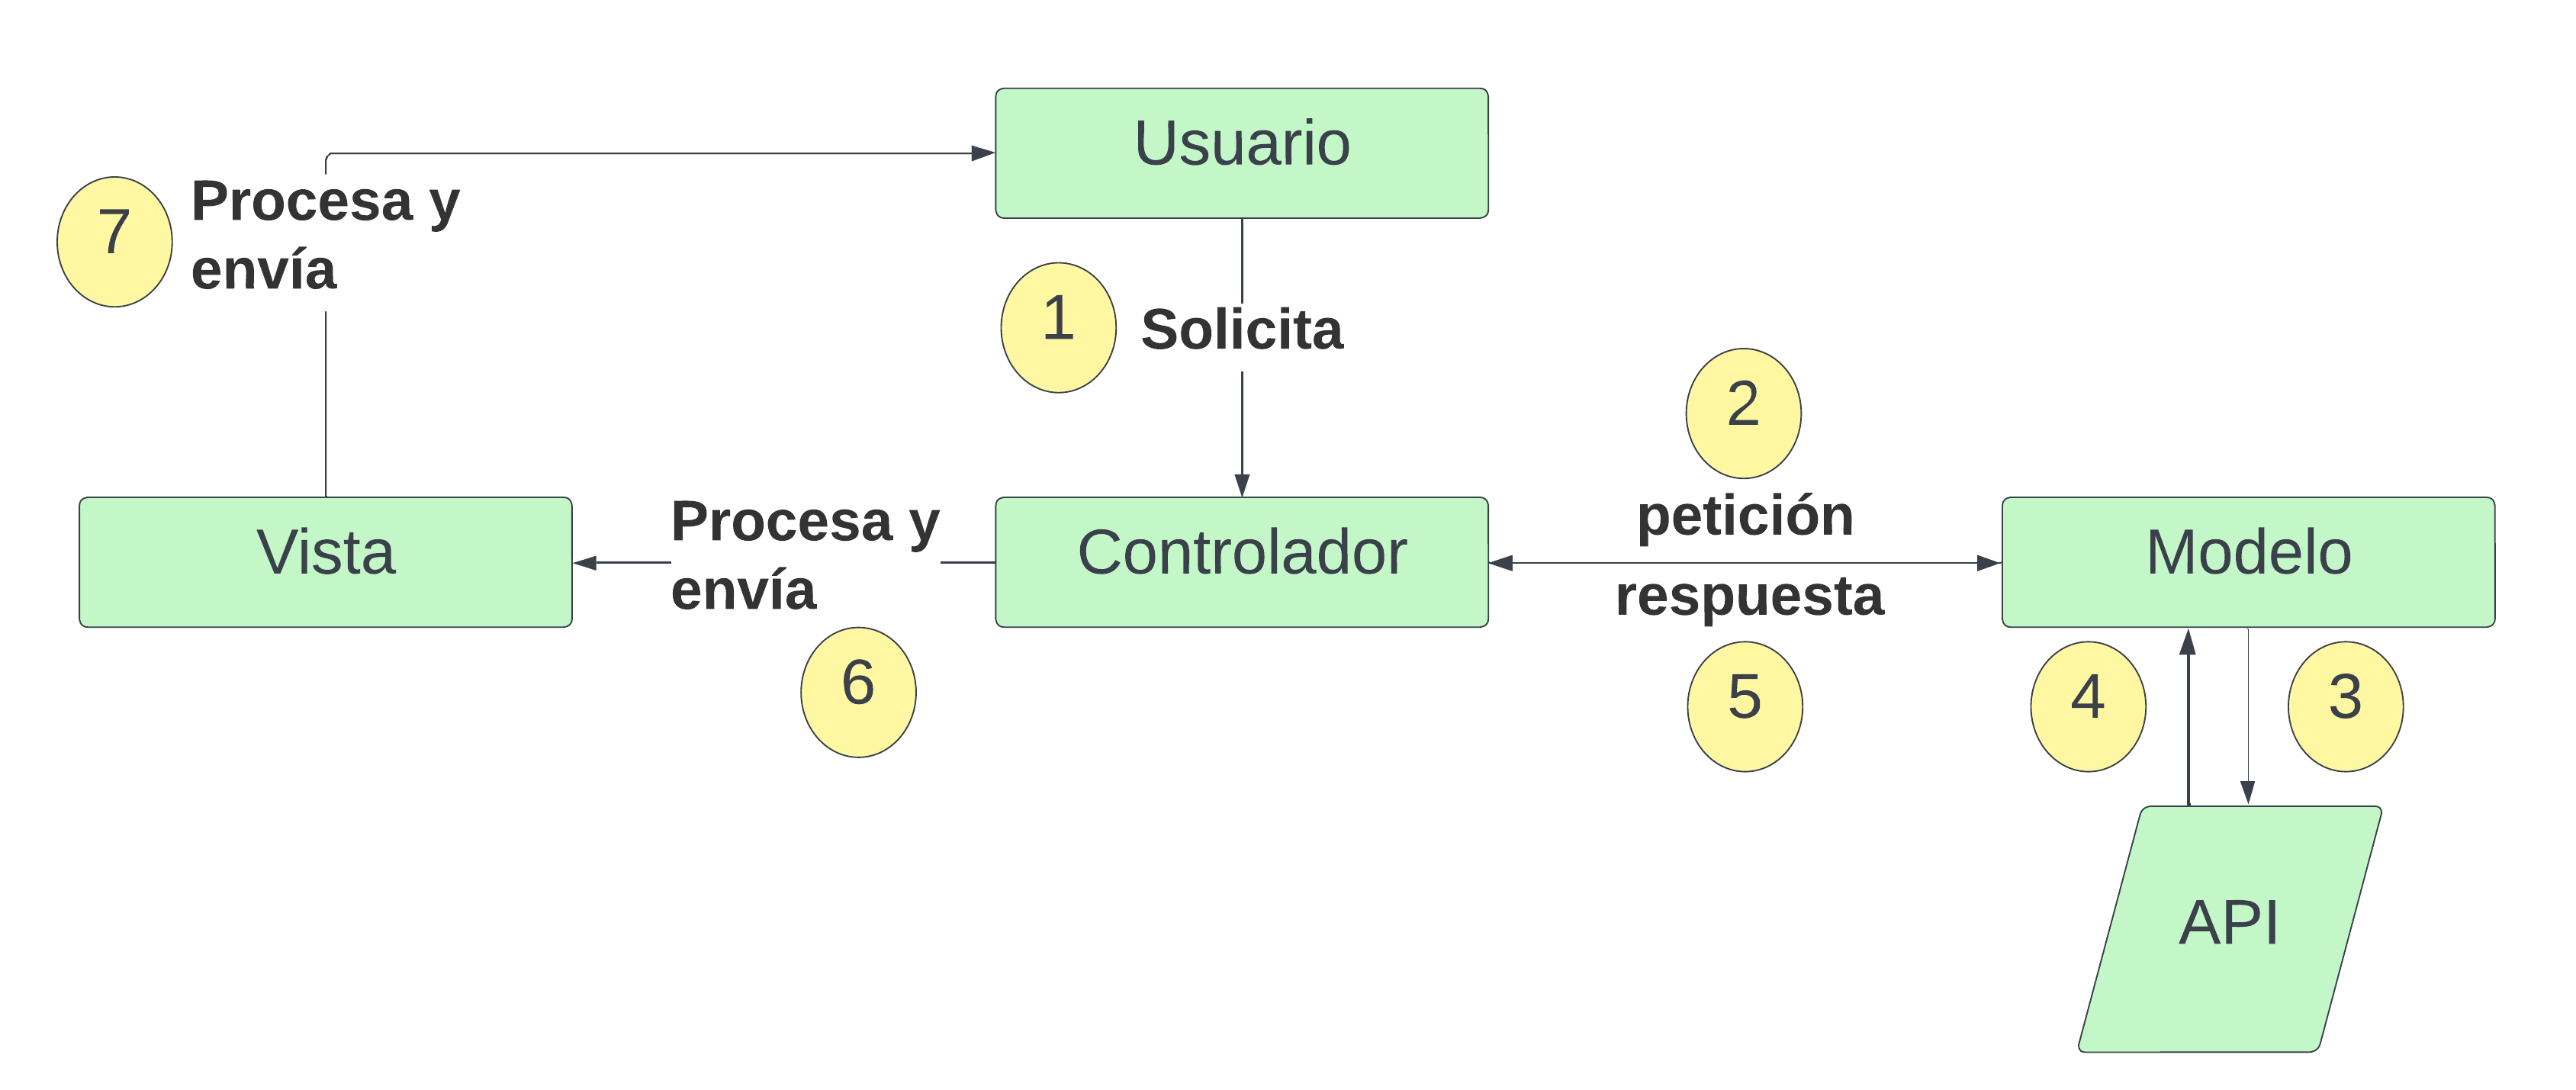
\includegraphics[width=\textwidth]{./Figures/front-mvc.png}
	\caption{Flujo en MVC.}
	\label{fig:frontmvc}
\end{figure}

Por ejemplo, para el desarrollo del módulo de listar ordenes de trabajo implementando este patrón, el flujo sería el siguiente:

\begin{enumerate}
\item El usuario solicita a través de su navegador la URL \textit{ordenestrabajo/listar}.
\item El \textit{routing} mapea la URL al controlador \textit{listar.page.ts} que se encuentra en el módulo \textit{listar.module.ts}. El controlador llama al servicio \textit{ordentrabajo.services.ts}.
\item El servicio hace una petición HTTP por medio del método GET a una ruta de la API de backend. 
\item La API responde con los datos de la lista en formato JSON.
\item El servicio entrega esos datos al controlador en formato JSON.
\item El controlador procesa los datos, realiza validaciones y filtros necesarios, ordena los datos, etc.
\item La vista procesa los datos, los inserta en una tabla, aplica los diseños CSS, etc. Luego envía la vista con los datos al usuario quien la visualizará en su navegador. 
\end{enumerate}

De esta manera se implementó este patrón de desarrollo para todos los componentes y módulos del frontend.

\subsection{Interfaces de usuario}
\label{subsec:frontinterfaces}

Teniendo en cuenta el flujo general del sistema presentado en el capítulo \ref{sec:flujogeneral} y los requerimientos para un sistema que sea amigable con el usuario y de diseño adaptable a diferentes dispositivos, se desarrollaron las interfaces de usuario utilizando los componentes nativos de Ionic para diseño de interfaces junto a CSS para personalizar estilos y javascript para funcionalidades. 

Las interfaces de usuario que se desarrollaron fueron:

\begin{enumerate}
\item Nueva: para añadir una nueva orden de trabajo.
\item Listar: para listar todas las ordenes de trabajo.
\item Retirar: para retirar una orden de trabajo.
\item Clientes: de tipo modal, para añadir o buscar un cliente.
\item Motos: de tipo modal, para añadir o buscar una motocicleta.
\item QR: para mostrar el código QR para autenticación en WhatsApp.
\end{enumerate}

\subsubsection{Nueva orden de trabajo}
\label{subsubsec:frontnuevaorden}
En la figura \ref{fig:nuevafull1} se puede observar los primeros campos del formulario a rellenar para cargar una nueva orden de trabajo.

\begin{figure}[H]
	\centering
	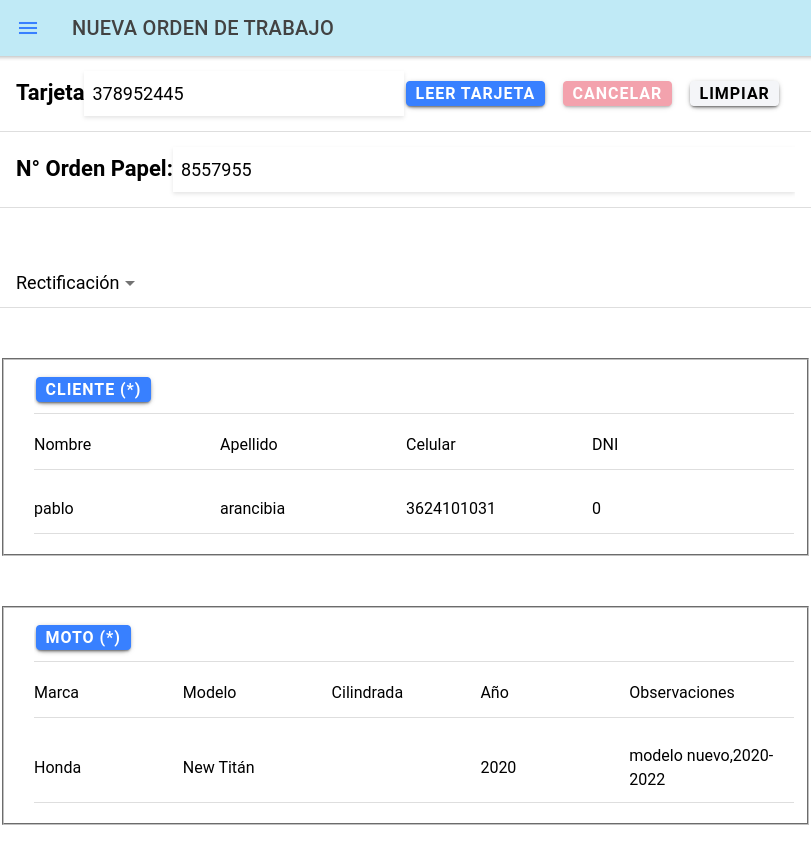
\includegraphics[scale=.40]{./Figures/nueva-full-1.png}
	\caption{Interfaz de usuario para nueva orden de trabajo.}
	\label{fig:nuevafull1}
\end{figure}


El usuario deberá hacer clic en el botón ``LEER TARJETA`` y luego pasar la tarjeta RFID por el lector ``mostrador``. De esta manera el sistema trae el número de tarjeta que fue seleccionada para asignar a la orden. Luego deberá cargar, si existe, un número de orden de manera manual el cual corresponde a un \textit{ticket} que usa actualmente la empresa.

Para una mejor experiencia de usuario se utilizan interfaces de tipo modal para cargar el tipo de trabajo, datos del cliente y la motocicleta.

En la figura \ref{fig:nuevatrabajo} se presenta la interfaz de tipo modal para seleccionar el tipo de trabajo a asignar a la orden.

\begin{figure}[H]
	\centering
	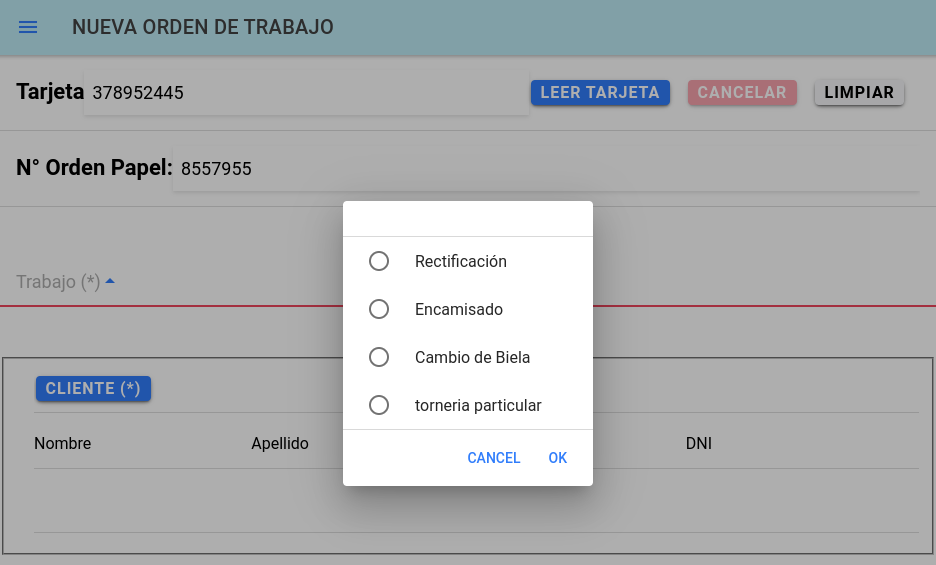
\includegraphics[scale=.40]{./Figures/nueva-trabajo.png}
	\caption{Interfaz de usuario de tipo modal para seleccionar tipo de trabajo.}
	\label{fig:nuevatrabajo}
\end{figure}

Para cargar o buscar los datos de clientes se utilizó el mismo componente, reutilizando así parte del código fuente. Como se puede ver en las figuras \ref{fig:nuevacliente1} y \ref{fig:nuevacliente2}, también se usa el tipo de interfaz modal.

\begin{figure}[H]
	\centering
	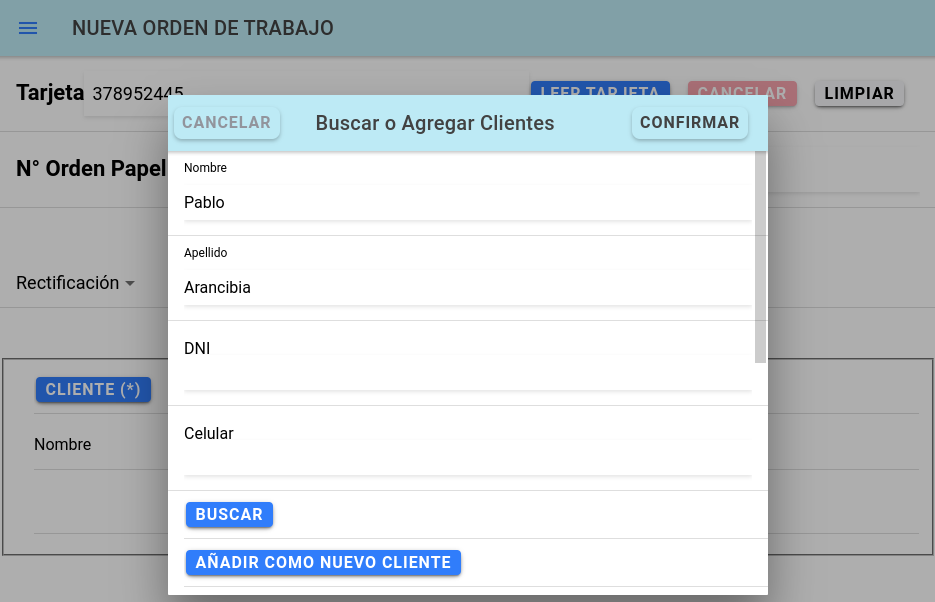
\includegraphics[scale=.40]{./Figures/nueva-clientes-1.png}
	\caption{Interfaz de usuario de tipo modal para seleccionar o buscar cliente.}
	\label{fig:nuevacliente1}
\end{figure}

En la figura \ref{fig:nuevacliente2} se puede observar el resultado de una búsqueda de clientes. Se selecciona el que se desea asignar y se hace clic en ``CONFIRMAR``.

\begin{figure}[H]
	\centering
	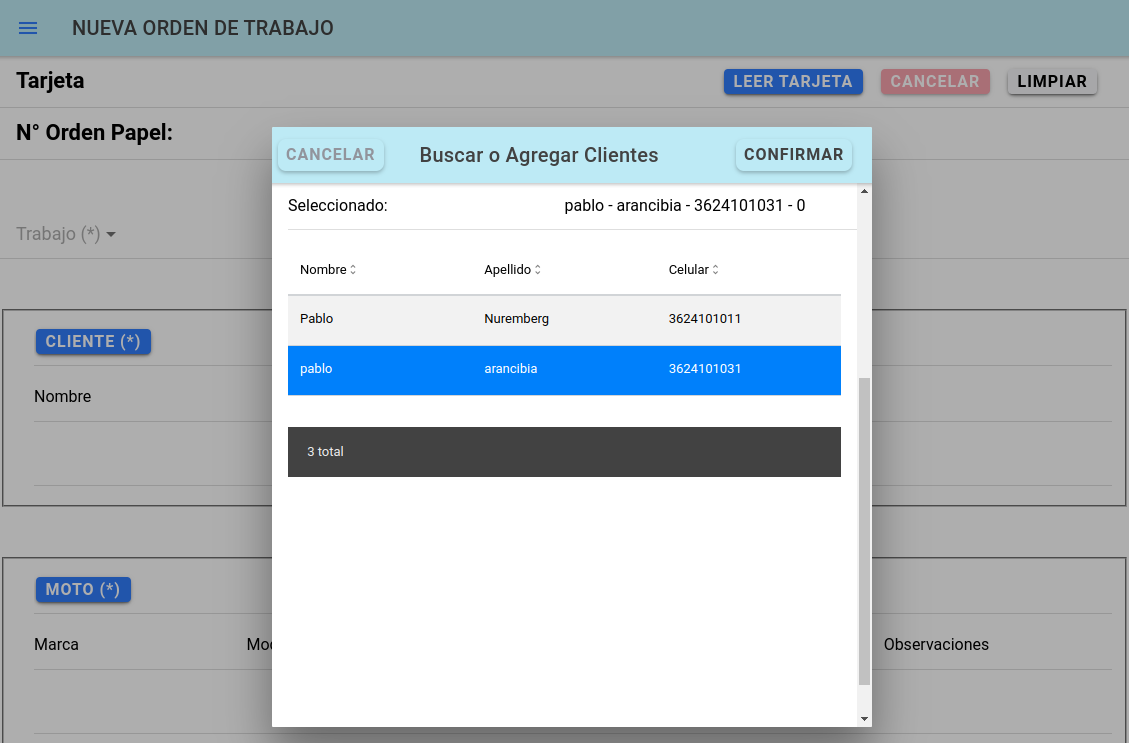
\includegraphics[scale=.30]{./Figures/nueva-clientes-2.png}
	\caption{Interfaz de usuario de tipo modal con el resultado de búsqueda de clientes.}
	\label{fig:nuevacliente2}
\end{figure}

De la misma manera se puede seleccionar o crear un registro de datos de una nueva motocicleta para asignar a la orden. En las figuras \ref{fig:nuevamoto1} y \ref{fig:nuevamoto2} se pueden observar las interfaces modales.


\begin{figure}[H]
	\centering
	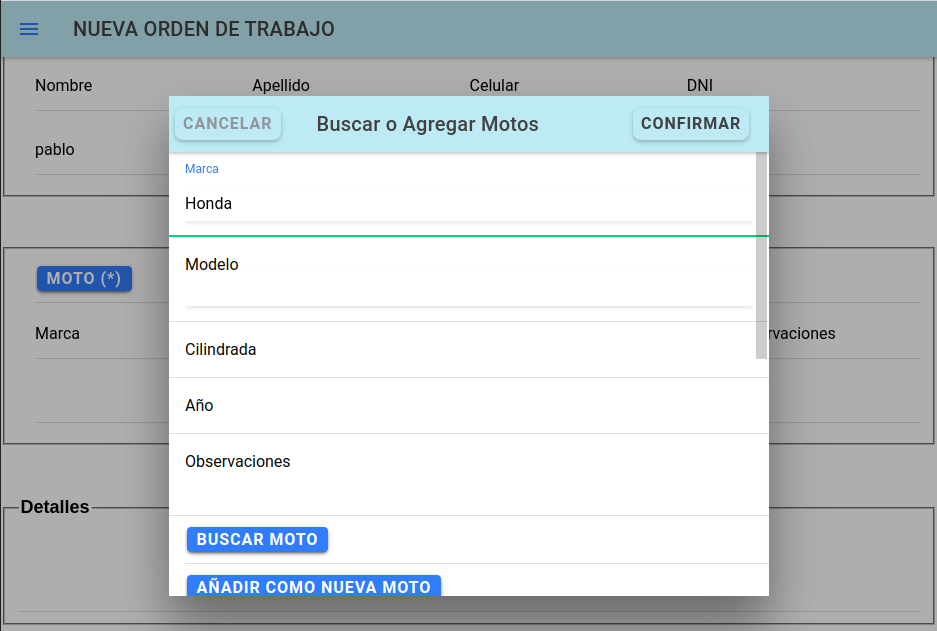
\includegraphics[scale=.35]{./Figures/nueva-moto-1.png}
	\caption{Interfaz de usuario de tipo modal para seleccionar o buscar motocicleta.}
	\label{fig:nuevamoto1}
\end{figure}

\begin{figure}[H]
	\centering
	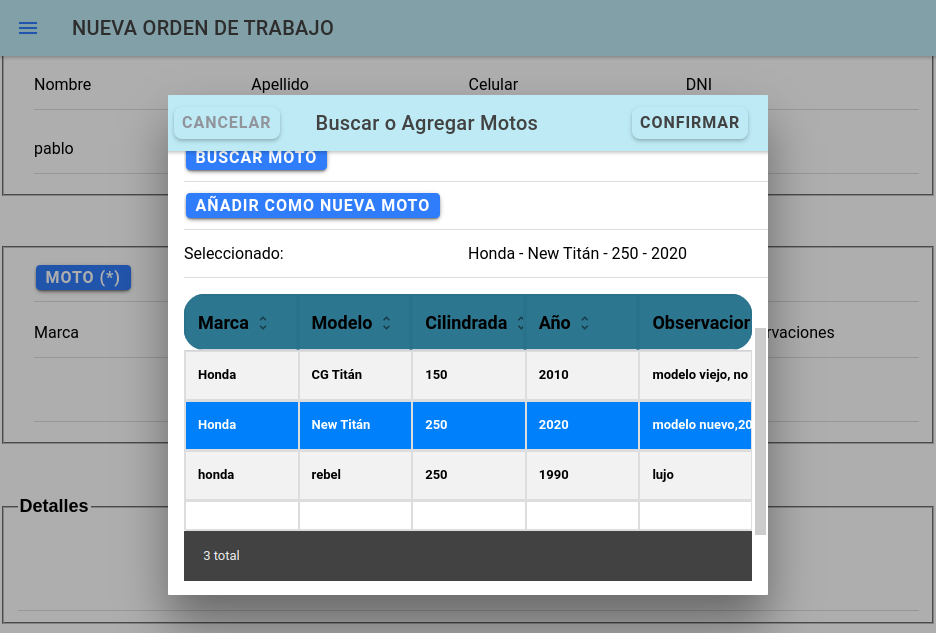
\includegraphics[scale=.35]{./Figures/nueva-moto-2.png}
	\caption{Interfaz de usuario de tipo modal con el resultado de búsqueda de motocicletas.}
	\label{fig:nuevamoto2}
\end{figure}

Volviendo a la segunda sección del formulario para agregar una nueva orden, ya habiendo cargado el número de tarjeta, el tipo de trabajo, el cliente y la motocicleta, se continúa con los campos que se representan en la figura \ref{fig:nuevafull2}.

 
\begin{figure}[H]
	\centering
	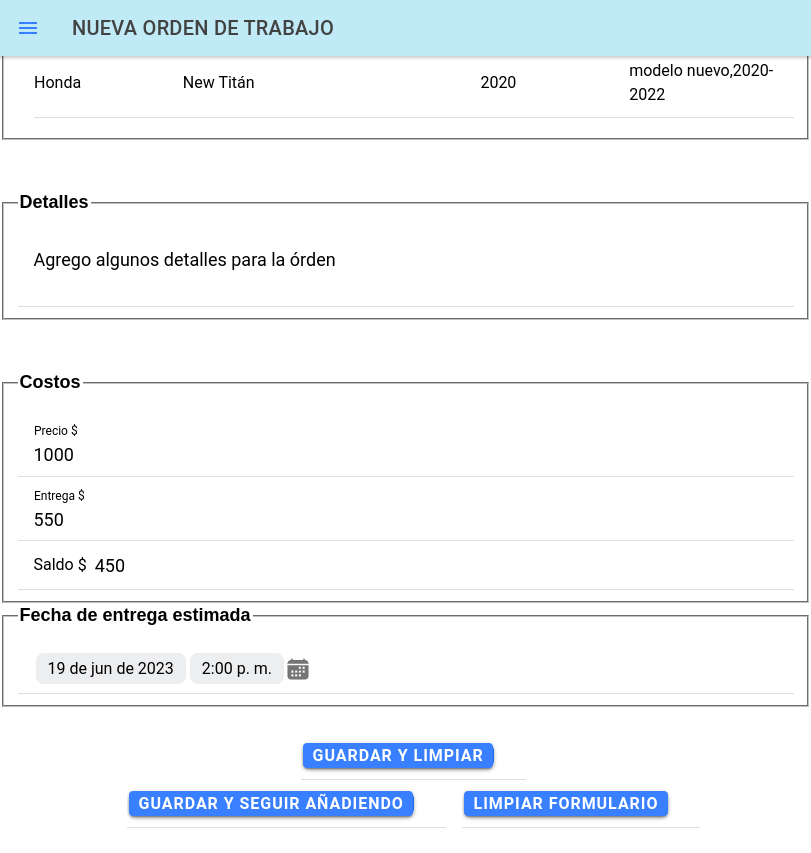
\includegraphics[scale=.35]{./Figures/nueva-full-2.png}
	\caption{Interfaz de usuario para nueva orden de trabajo.}
	\label{fig:nuevafull2}
\end{figure}

En esta sección se pueden agregar detalles, costos y fecha de entrega estimada.

\begin{itemize}
\item Detalles: para agregar algunas observaciones a la orden en formato de texto
Costos: están separados en 3 campos: el precio total de la orden, la entrega que realiza el cliente cuando deja el repuesto y el saldo restante. 
\item Fecha de entrega estimada: al seleccionar la fecha saldrá un calendario de tipo modal para seleccionar el día y la hora de entrega. 
\end{itemize}


Por último sólo queda guardar la orden, para ello se pueden realizar dos acciones: 

\begin{itemize}
\item GUARDAR Y LIMPIAR: esta opción se utilizará cuando el cliente sólo deje un repuesto para trabajar de manera tal que se guarda el registro y se limpia completamente el formulario

\item GUARDAR Y SEGUIR AÑADIENDO: cuando el mismo cliente tiene varios repuestos para dejar, de esta manera se guarda el registro pero se mantienen los datos del cliente en el formulario. 
\end{itemize}

La última opción corresponde a ``LIMPIAR FORMULARIO`` que borra los datos del formulario sin guardar ningún registro.


\subsubsection{Listar ordenes de trabajo}
\label{subsubsec:frontlistarordenes}

En la figura \ref{fig:listado1} se puede observar la interfaz gráfica para donde se listan las ordenes de trabajo según las opciones seleccionadas.

\begin{figure}[H]
	\centering
	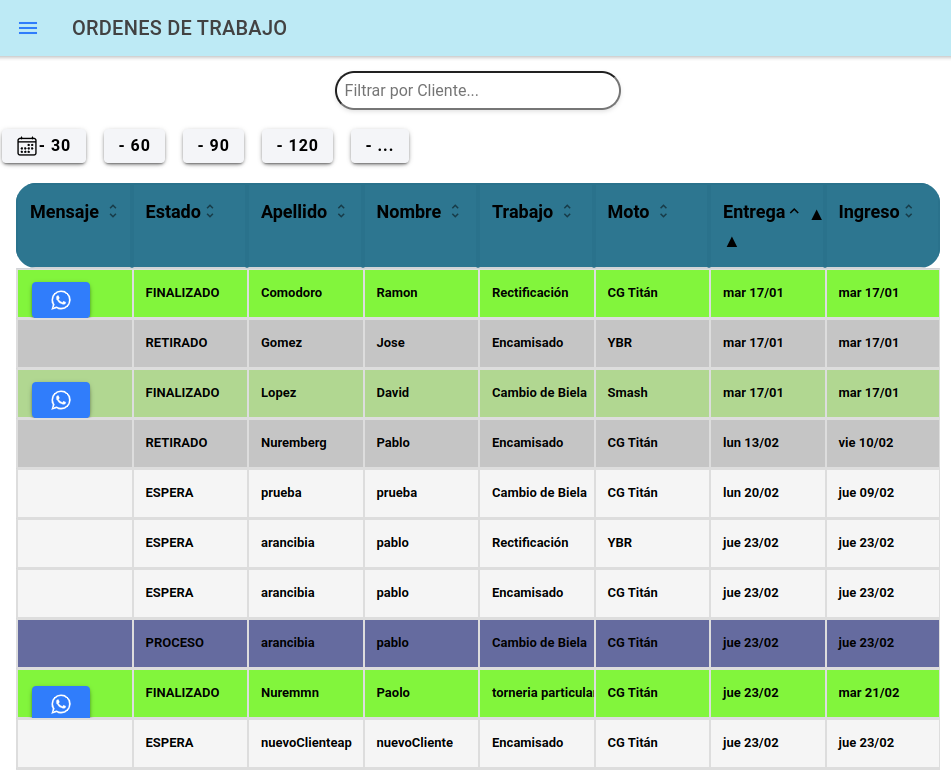
\includegraphics[scale=.40]{./Figures/listado-1.png}
	\caption{Interfaz de usuario para listar las ordenes de trabajo.}
	\label{fig:listado1}
\end{figure}

Las opciones en esta interfaz son:

\begin{itemize}
\item Filtrado: se puede filtrar por cualquier campo de la tabla, una vez que se filtran los resultados, la información se sigue actualizando en tiempo real, por lo que si una fila cambia de estado, se verá de todas maneras el cambio.

\item Rango de días: en la parte superior de la tabla se pueden observar 5 botones, estos representan al rango de días hacia atrás que se desea mostrar los registros. Además la tabla muestra al usuario una paginación navegable en la parte inferior si los registros son mayores a 25. El último botón de este grupo corresponde a mostrar el historial completo de registros.

\item Ordenamiento por campos: al hacer clic en la cabecera de la tabla se puede ordenar los elementos de manera múltiple, por ejemplo en primer orden la fecha de entrega y en segundo orden el apellido del cliente, así sucesivamente en múltiples campos.

\item orden de columnas: se pueden ordenar los campos haciendo clic y arrastrando el campo deseado al orden correspondiente. Por ejemplo se puede arrastrar el campo ``Estado`` en la primera columna.
\end{itemize}

Para una mejor visualización de los estados de los trabajos se asignó un color específico para cada estado, de esta manera es más fácil identificar rápidamente el estado de los trabajos. Se utilizó la siguiente paleta de colores para los estados:

\begin{itemize}
\item Espera: color verde.
\item Proceso: color púrpura.
\item Finalizado: color verde brillante o verde opaco.
\item Retirado: color gris. 
\end{itemize} 

Además se asigna un botón en la columna ``Mensaje``, solamente a las filas de los trabajos que están en estado ``FINALIZADO``. Este botón tiene el logo de la aplicación WhatsApp y se utiliza para enviar un mensaje al cliente informando que su trabajo está finalizado y listo para retirarse. En caso que el cliente todavía no fue alertado el color de la fila será verde brillante, si el cliente ya fue avisado el color de la fila será verde opaco. El usuario puede reenviar un mensaje a un cliente si lo desea sólo que el sistema lo alertará previamente.

En las figuras \ref{fig:listado2} y \ref{fig:listado3} se representan los alertas de tipo modal que se utilizan para confirmar cuando el usuario va a enviar o reenviar un mensaje a un cliente.

\begin{figure}[H]
	\centering
	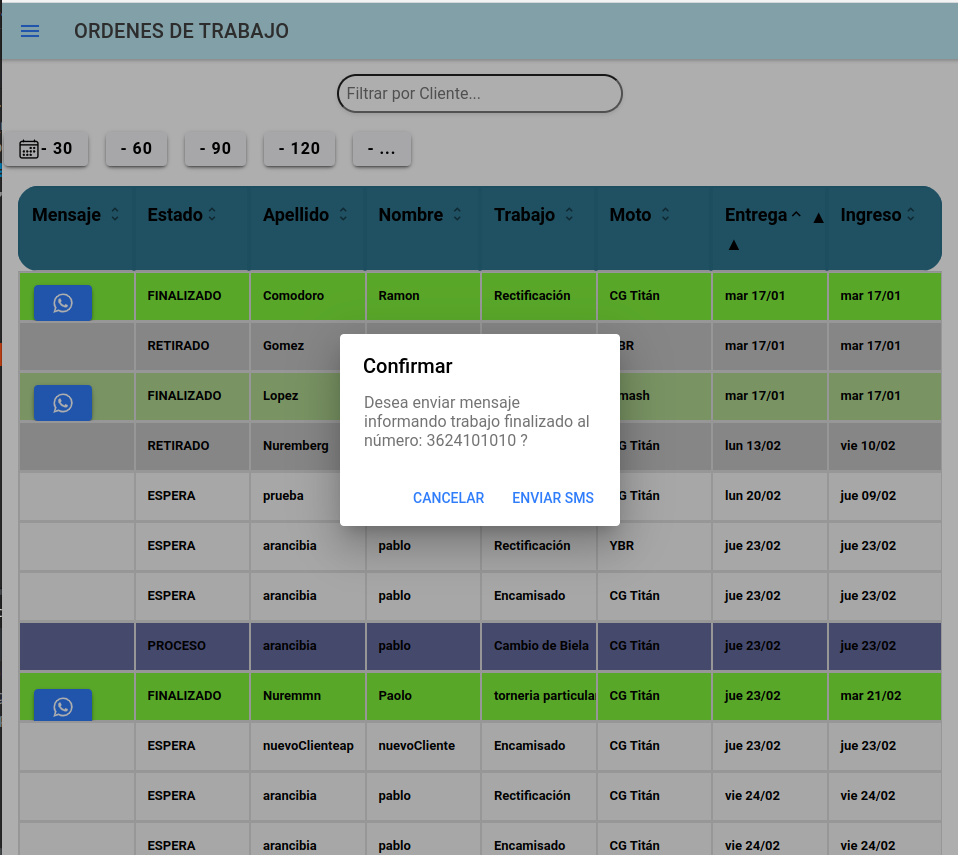
\includegraphics[scale=.35]{./Figures/listado-2.png}
	\caption{Interfaz para confirmar envío de mensaje de texto al cliente.}
	\label{fig:listado2}
\end{figure}

\begin{figure}[H]
	\centering
	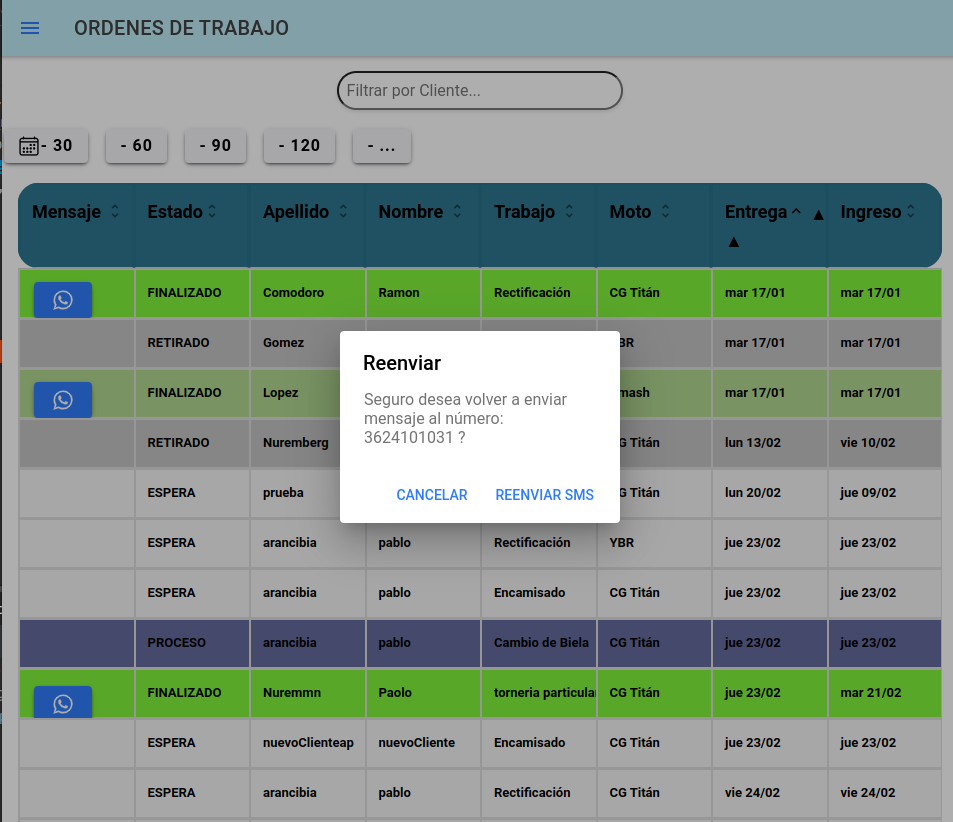
\includegraphics[scale=.35]{./Figures/listado-3.png}
	\caption{Interfaz para confirmar reenvío de mensaje de texto al cliente.}
	\label{fig:listado3}
\end{figure}

Como se detalló en el capítulo \ref{sec:apimessenger} el mensaje llegá al cliente en su aplicación WhatsApp como si fuera enviado desde el teléfono móvil del usuario, por lo que mostrará su número o el nombre por el cual el cliente lo tenga agendado, ya que la API de mensajería utiliza los servicios de WhatsApp para hacer el envío y el usuario debe autenticarse previamente con su teléfono móvil y el código QR para utilizar el servicio.

\subsubsection{Retirar orden de trabajo}
\label{subsubsec:frontretirar}

Para retirar una orden se utiliza una metodología similar a la de agregar una nueva orden de trabajo. El usuario va hacer clic en un botón para activar la búsqueda de un evento, este evento será pasar la tarjeta RFID del repuesto por el nodo mostrador, una vez hecho esto el número de la tarjeta con todos los datos de la orden se cargará en la pantalla. 

El usuario puede modificar el precio de la orden en este punto y se actualizarán los datos de saldo. También puede agregar detalles para el retiro de la orden que quedarán registrados en la base de datos.

Una vez confirmado el retiro se guardan los registros y estados correspondientes y se asigna el estado ``libre`` a la tarjeta para que pueda ser reutilizada para una futura orden de trabajo.

De esta manera finaliza el ciclo de un repuesto que ingresa a la empresa, es procesado y retirado luego por el cliente.

En las figuras \ref{fig:retirar1} y \ref{fig:retirar2} se muestra la interfaz para retirar una orden de trabajo.

\begin{figure}[H]
	\centering
	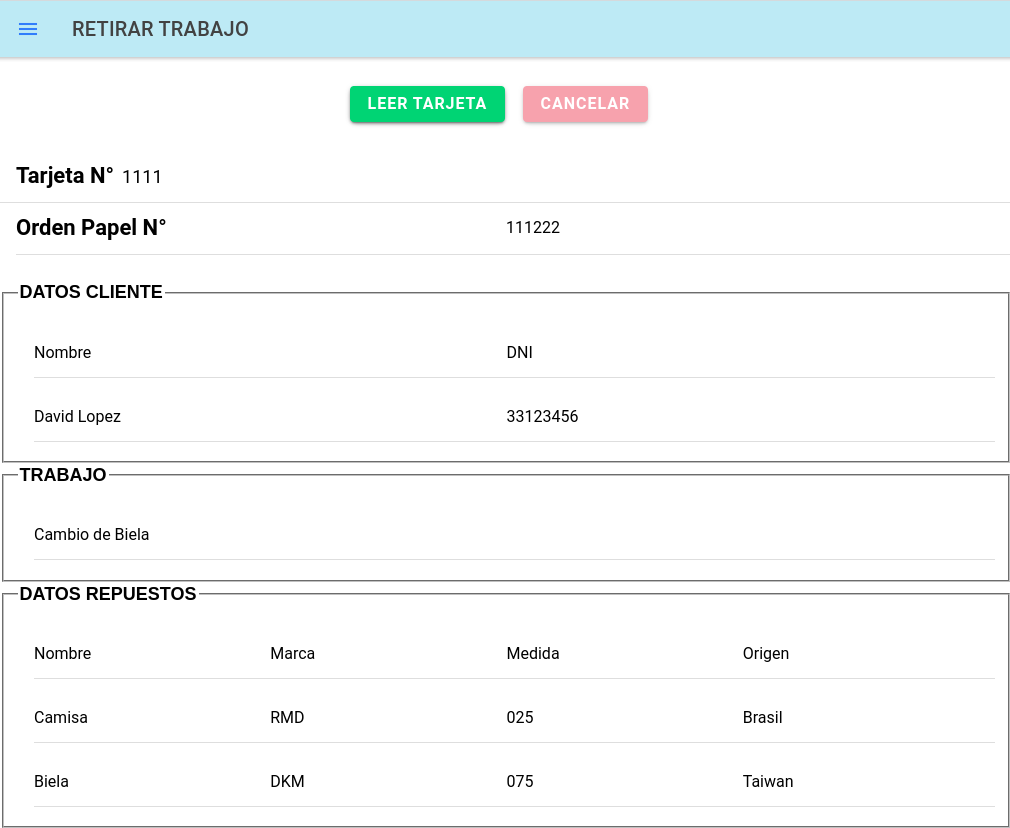
\includegraphics[scale=.35]{./Figures/retirar-1.png}
	\caption{Formulario para retirar orden de trabajo.}
	\label{fig:retirar1}
\end{figure}

\begin{figure}[H]
	\centering
	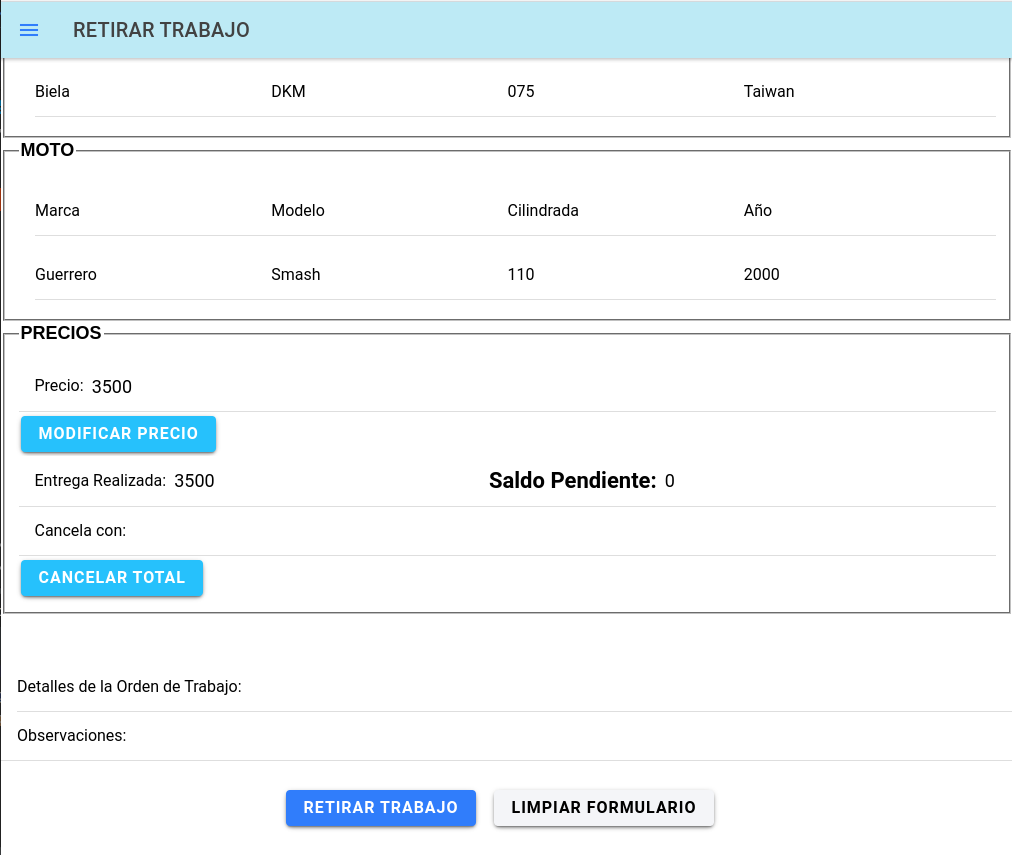
\includegraphics[scale=.35]{./Figures/retirar-2.png}
	\caption{Confirmar retiro de orden de trabajo.}
	\label{fig:retirar2}
\end{figure}

\subsubsection{Autenticación a API de mensajería}
\label{subsubsec:frontqr}

Para la autenticación a la API de mensajería se utiliza un código QR que se obtiene consultando dicha API por protocolo HTTP. La misma devuelve un archivo SVG que se muestra en la interfaz gráfica del usuario para que pueda ser escaneada por su teléfono móvil y de esta manera acceder a las funciones de envío de mensajes a clientes.

En la figura \ref{fig:frontqr} se muestra la interfaz para autenticarse mediante código QR. También se puede observar el botón ``ACTUALIZAR`` para refrescar el código por uno nuevo´.

\begin{figure}[H]
	\centering
	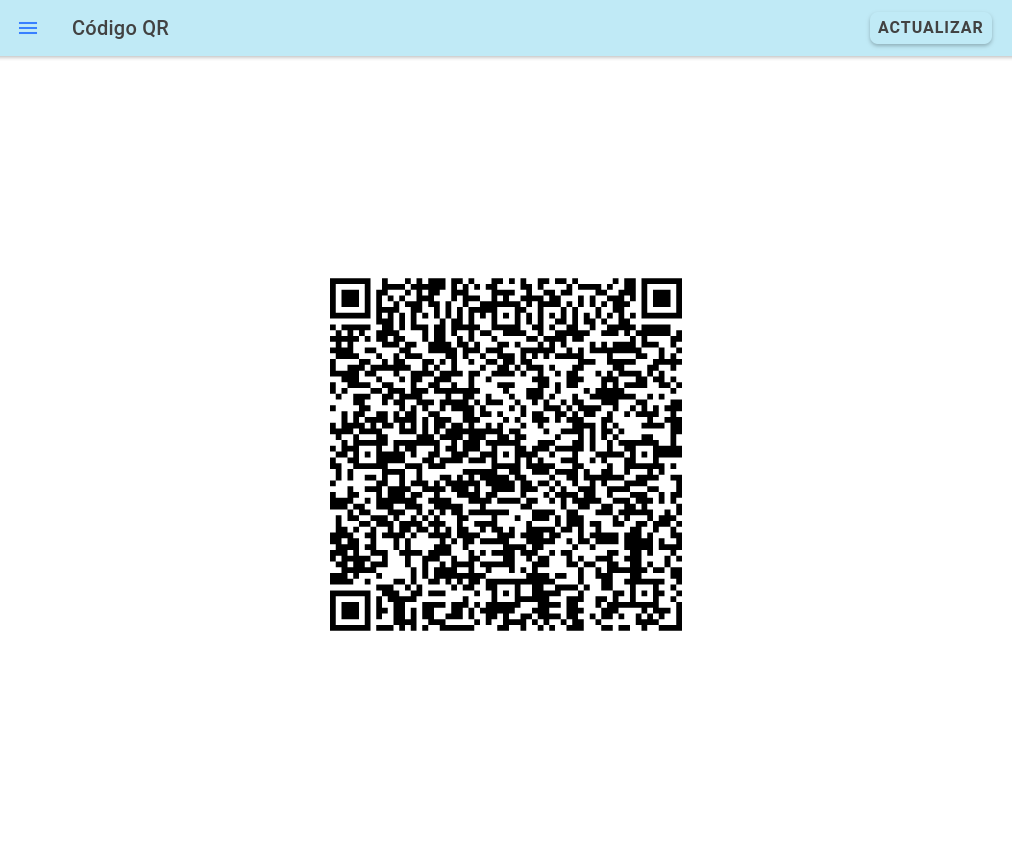
\includegraphics[scale=.30]{./Figures/qr-page.png}
	\caption{Interfaz para autenticación en API de mensajería.}
	\label{fig:frontqr}
\end{figure}

\section{Arquitectura de servidor}
\label{sec:server}

Para el despliegue de los servicios desarrollados se implementó una arquitectura de contenedores utilizando Docker y Docker Compose en una Raspberry Pi 4.

Para cada proyecto se creó un archivo Dockerfile para el manejo del contenedor correspondiente, a su vez se centraliza el despliegue de estos contenedores en un archivo \textit{yml} de Docker Compose, donde también se levantan servicios directamente sin utilizar un Dockerfile particular. 

En esta sección se detalla la implementación de contenedores y servicios en el servidor.

\subsection{Implementación de contenedores}
\label{subsec:contenedores}

A continuación, en el código \ref{cod:dockercompose}, se representa el código fuente utilizado en Docker Compose para el despliegue de todos los contenedores de cada proyecto o servicio utilizado.

\begin{lstlisting}[label=cod:dockercompose,caption=Código de Docker Compose.]
version: '3'

services:
    db:
        container_name: mysqldb
        restart: always
        image: mysql
        env_file:
        - .env_mysql/.mysql.env
        volumes:
            - ./sql-data/db:/var/lib/mysql
        ports: 
            - "3306:3306"
    api:
         depends_on: 
             - db 
         container_name: backendapi
         restart: always
         build:
             context: .
             dockerfile: Dockerfile
         command: bash -c 'while !</dev/tcp/db/3306; do sleep 1; done; npm run dev'
         ports:
             - "3001:3001"
         env_file:
         - ./api/.env
         volumes:
             - ./:/app
    mosquitto:
        image: eclipse-mosquitto
        container_name: mosquittobroker
        ports:
            - "1883:1883"
            - "9001:9001"
        volumes:
        - './mqtt/etc/mosquitto.conf:/mosquitto/config/mosquitto.conf'
        - './mqtt/etc/mqttusers:/mosquitto/config/mqttusers'
        - './mqtt/data:/mosquitto/data'
        - './mqtt/log:/mosquitto/log'
        restart: always
    web:
        container_name: web
        restart: always
        build:
            context: .
            dockerfile: Dockerfile-frontend
        ports:
            - "80:80"
    messenger:
         container_name: messenger
         restart: always
         build:
             context: api-whatsapp-ts
             dockerfile: Dockerfile
         ports:
             - "3003:3003"
         volumes:
             - ./:/messenger
    portainer:
        image: portainer/portainer-ce
        restart: always
        ports:
            - "9000:9000"
        volumes:
            - /var/run/docker.sock:/var/run/docker.sock
            - portainer_data:/data
volumes:
    portainer_data:
\end{lstlisting}  

A continuación se describen cada uno de los servicios para la aplicación:

\begin{itemize}

\item db: este servicio utiliza la imagen de Docker para crear un contenedor de base de datos MySQL. Se le asigna un nombre de contenedor \textit{mysqldb}, se establece una opción de reinicio siempre que se detiene, se define un archivo .env para configurar las variables de entorno, se mapea un volumen local a la ruta de datos de MySQL y se expone el puerto 3306.

\item api: este servicio es la API de la aplicación para el backend. Su ejecución depende del servicio de la base de datos \textit{db} y utiliza un archivo .env para configurar las variables de entorno. Se construye a partir de un archivo Dockerfile. Se mapea al puerto 3001.

\item mosquitto: este servicio utiliza la imagen de Docker \textit{eclipse-mosquitto} para crear un contenedor de un servidor MQTT. Se le asigna un nombre de contenedor \textit{mosquittobroker}, se expone los puertos 1883 y 9001, se mapea la configuración y los datos de MQTT a un volumen local y se establece una opción de reinicio siempre que se detiene.

\item web: este servicio es la interfaz \textit{web} de la aplicación la cual utiliza NGINX para servir la aplicación desarrollada en IONIC. Se construye a partir de un archivo Dockerfile en el directorio actual y se mapea el puerto 80.

\item messenger: este servicio utiliza un archivo Dockerfile en el directorio de la API de mensajería para crear un contenedor y servir la API. Se le asigna un nombre de contenedor \textit{messenger} y se mapea al puerto 3003.

\item portainer: este servicio utiliza la imagen de Docker \textit{portainer/portainer-ce} para crear un contenedor del administrador de Docker \textit{Portainer}. Se mapea el puerto 9000 y se utiliza un volumen para almacenar los datos. Se describe esta herramienta en el capítulo \ref{subsec:portainer}.
\end{itemize}

Al desplegar Docker Compose se levantan todos los servicios como se muestra en la figura \ref{fig:docker-interfaz}.

\begin{figure}[H]
	\centering
	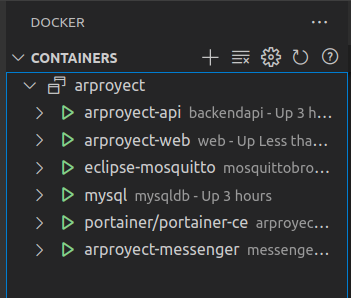
\includegraphics[scale=.60]{./Figures/docker-interfaz.png}
	\caption{Contenedores de Docker.}
	\label{fig:docker-interfaz}
\end{figure}

\section{Implementación de Hardware}
\label{sec:implementacionhw}

A continuación se describe la implementación del \textit{hardware} utilizado y detallado en el capítulo \ref{sec:hardware}.

Para el manejo de la red local se configuró un \textit{router} con una red Wi-Fi con filtrado de direcciones MAC y un servidor DHCP con entrega de IP fija a los dispositivos del sistema.

Al observar el diagrama de red en la figura \ref{fig:diagramared}, se puede obtener información detallada acerca de qué tipo de conexión utiliza cada dispositivo.

\begin{figure}[H]
	\centering
	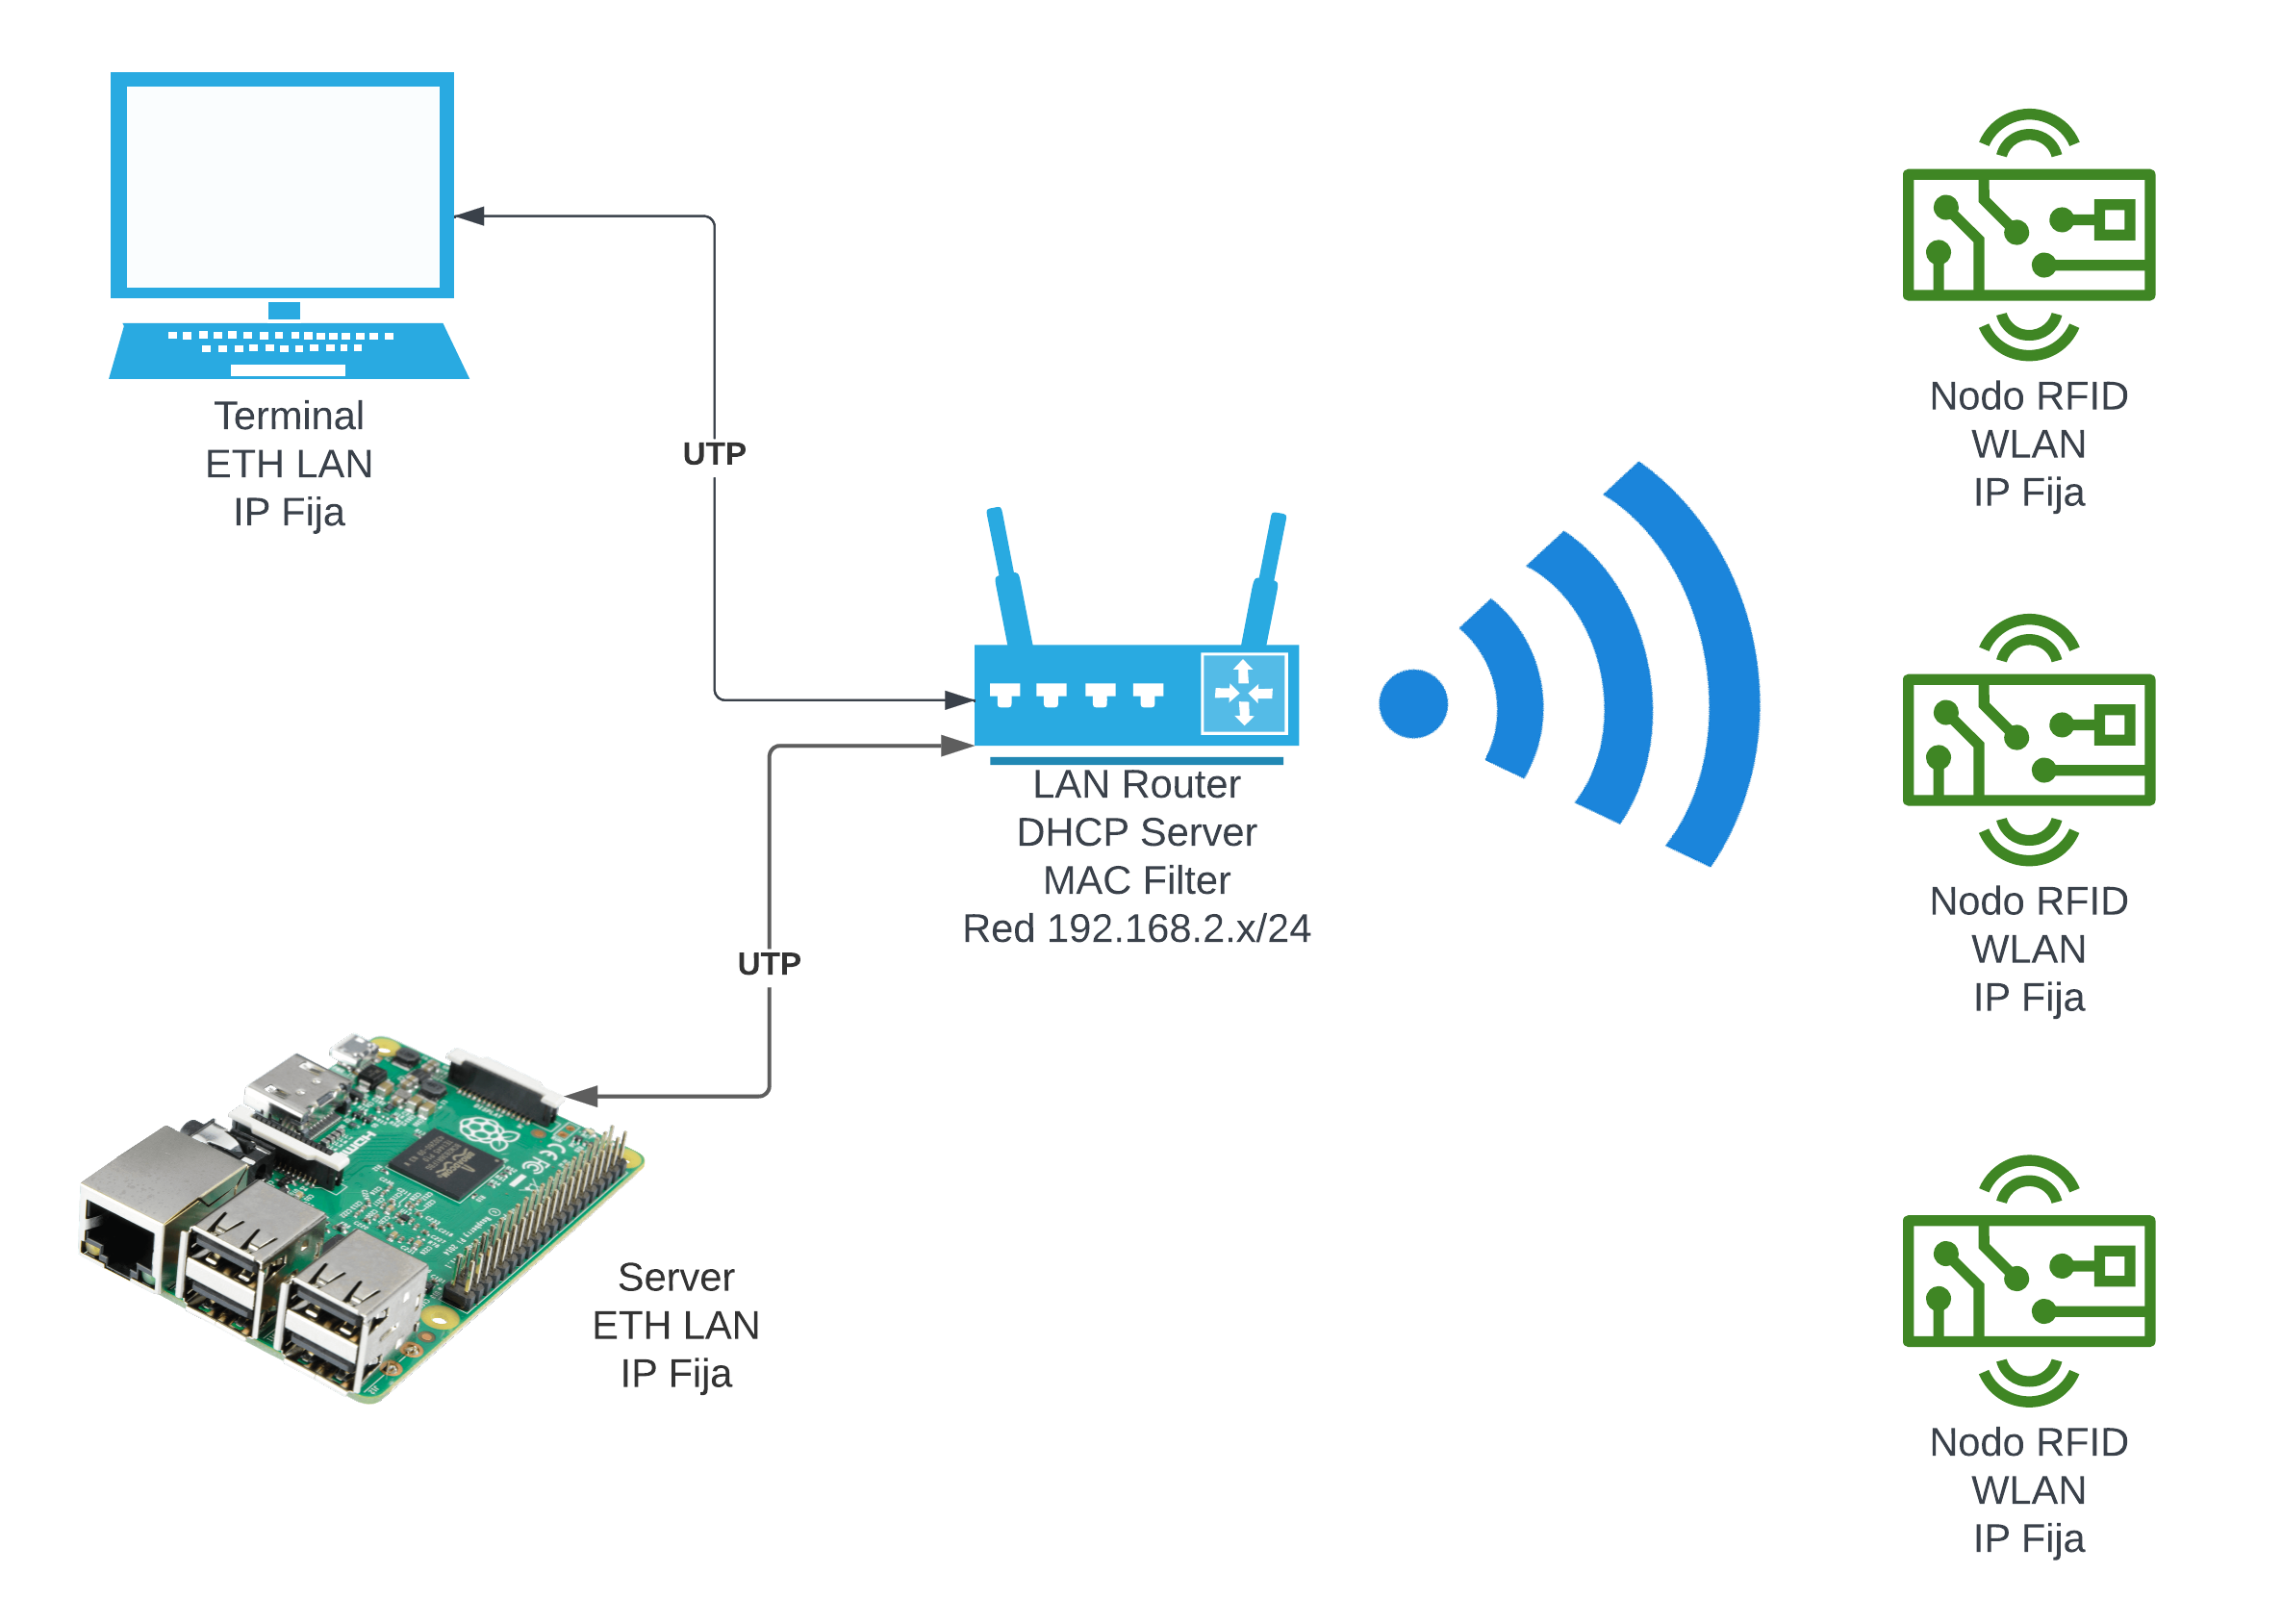
\includegraphics[width=\textwidth]{./Figures/diagrama-red.png}
	\caption{Diagrama de red del sistema.}
	\label{fig:diagramared}
\end{figure}

En el servidor se implementó una placa Raspberry Pi 4. Para esta placa se imprimió un gabinete personalizado utilizando una impresora de tipo 3D, se incluyó además un espacio adicional en el gabinete para agregar un disco tipo SSD para ampliar las capacidades de la placa. En la figura \ref{fig:rbcase} se puede observar el gabinete personalizado.

\begin{figure}[H]
	\centering
	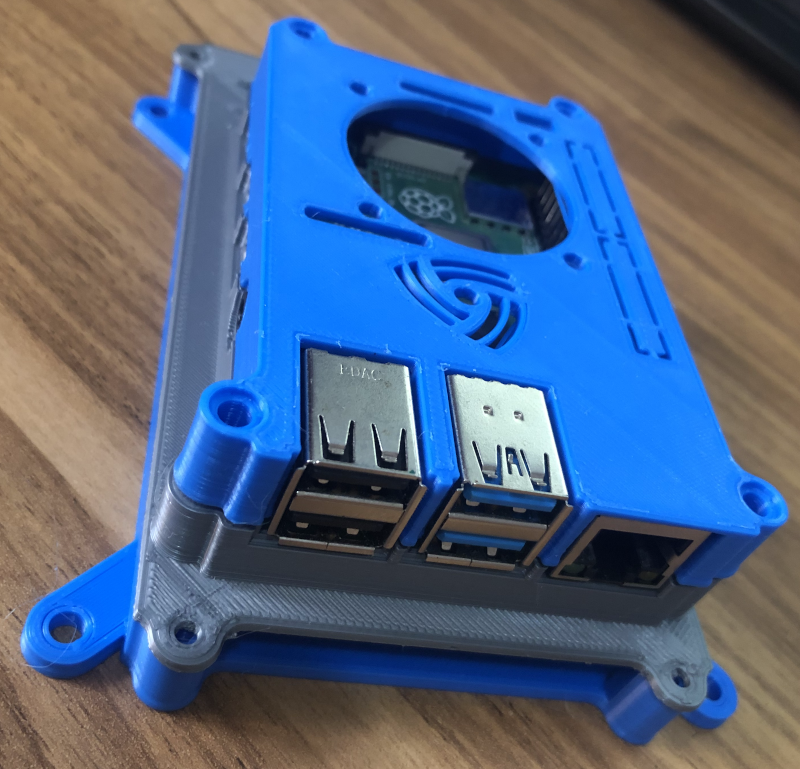
\includegraphics[scale=.30]{./Figures/hardware/rbcase.png}
	\caption{Case de Raspberry Pi con \textit{slot} para SSD.}
	\label{fig:rbcase}
\end{figure}


Para los nodos se utilizó el microcontrolador NodeMCU ESP32, el sensor de radiofrecuencia MRC522 y un \textit{buzzer} sonoro. El diseño del circuito electrónico y la impresión de la placa PCB estuvo a cargo de colaboradores.

En la figura \ref{fig:hwesquematico} se puede observar el diseño del circuito utilizado para los nodos.

\begin{figure}[H]
	\centering
	\includegraphics[width=\textwidth]{./Figures/hardware/esquematico.png}
	\caption{Circuito esquemático para placa PCB.}
	\label{fig:hwesquematico}
\end{figure}

En la figura \ref{fig:hwlayout} se observa el diseño del circuito impreso para la placa PCB. 

\begin{figure}[H]
	\centering
	\includegraphics[scale=.35]{./Figures/hardware/layout.png}
	\caption{Circuito impreso para placa PCB.}
	\label{fig:hwlayout}
\end{figure}  

En la figura \ref{fig:hwnodo} se observan los componentes del nodo y la placa PCB.

\begin{figure}[H]
	\centering
	\includegraphics[scale=.40]{./Figures/hardware/nodo.png}
	\caption{Componentes y placa PCB para nodos.}
	\label{fig:hwnodo}
\end{figure}


Para realizar el \textit{build} o compilación del código fuente en el microcontrolador NodeMCU ESP32 se utilizó el \textit{framework} PlatformIO \cite{platformio} y el IDE Visual Studio Code (VSCode) \cite{vscode}.

En la figura \ref{fig:platformio-build} se puede observar el resultado de realizar el \textit{build}  o compilación del código fuente en la ESP32 utilizando PlatformIO y VSCode.

\begin{figure}[H]
	\centering
	\includegraphics[width=\textwidth]{./Figures/platformio-build.png}
	\caption{Terminal de VSCode, build en PlatformIO.}
	\label{fig:platformio-build}
\end{figure}

En la figura \ref{fig:platformio-upload} se observa el resultado de realizar el \textit{upload} o el copiado del código ya compilado a la ESP32 en PlatformIO. Además se detalla la instalación de las librerías que se utilizan en el proyecto.

\begin{figure}[H]
	\centering
	\includegraphics[width=\textwidth]{./Figures/platformio-upload.png}
	\caption{Terminal de VSCode, upload en PlatformIO.}
	\label{fig:platformio-upload}
\end{figure}

Finalmente, en la figura \ref{fig:platformio-connect} se muestra el resultado del código fuente ejecutándose en el microcontrolador y los detalles de la conexión exitosa a la red Wi-Fi y al \textit{broker} MQTT, indicando las direcciones IP y los puertos de conexión, además se muestran los mensajes que se configuraron en el código como el nombre de usuario y del nodo, la dirección IP y MAC de la ESP32 y el tópico MQTT al cual está suscripto. Esto se realiza mediante el \textit{framework} PlatformIO en modo monitor y con la ESP32 conectada a la PC mediante un cable USB de datos.
 
\begin{figure}[H]
	\centering
	\includegraphics[width=\textwidth]{./Figures/platformio-connect.png}
	\caption{Terminal de VSCode, conexión en PlatformIO.}
	\label{fig:platformio-connect}
\end{figure}




% La idea de esta sección es resaltar los problemas encontrados, los criterios utilizados y la justificación de las decisiones que se hayan tomado.

% Se puede agregar código o pseudocódigo dentro de un entorno lstlisting con el siguiente código:

% \begin{verbatim}
% \begin{lstlisting}[caption= "un epígrafe descriptivo"]
% 	las líneas de código irían aquí...
% \end{lstlisting}
% \end{verbatim}

% A modo de ejemplo:

% \begin{lstlisting}[label=cod:vControl,caption=Pseudocódigo del lazo principal de control.]  % Start your code-block

% #define MAX_SENSOR_NUMBER 3
% #define MAX_ALARM_NUMBER  6
% #define MAX_ACTUATOR_NUMBER 6

% uint32_t sensorValue[MAX_SENSOR_NUMBER];		
% FunctionalState alarmControl[MAX_ALARM_NUMBER];	//ENABLE or DISABLE
% state_t alarmState[MAX_ALARM_NUMBER];						//ON or OFF
% state_t actuatorState[MAX_ACTUATOR_NUMBER];			//ON or OFF

% void vControl() {

% 	initGlobalVariables();
	
% 	period = 500 ms;
		
% 	while(1) {

% 		ticks = xTaskGetTickCount();
		
% 		updateSensors();
		
% 		updateAlarms();
		
% 		controlActuators();
		
% 		vTaskDelayUntil(&ticks, period);
% 	}
% }
% \end{lstlisting}




%	% Chapter Template

\chapter{Ensayos y resultados} % Main chapter title

\label{Chapter4} % Change X to a consecutive number; for referencing this chapter elsewhere, use \ref{ChapterX}

En este capítulo se explica cómo se hicieron los ensayos y qué resultados se obtuvieron.
%----------------------------------------------------------------------------------------
%	SECTION 1
%----------------------------------------------------------------------------------------

\section{Banco de pruebas}
\label{sec:entornos}

Se utilizaron 3 entornos para llevar a cabo el desarrollo y las consecuentes pruebas del sistema. A nivel de \textit{software} se administraron utilizando un repositorio en la nube y manteniendo 3 ramas individuales de código, una para cada entorno. A nivel de \textit{hardware} se fue escalando entre entornos a medida que se avanzaba en el desarrollo y las pruebas.

Los entornos se denominaron de la siguiente manera:
\begin{itemize}
\item dev: para referirse a \textit{development} o desarrollo.
\item test: para referirse a \textit{testing} o pruebas.
\item prod: para referirse a \textit{production} o producción.
\end{itemize}

En la figura \ref{fig:entornos} podemos observar cada entorno y las tareas realizadas en cada uno.

\begin{figure}[H]
	\centering
	\includegraphics[scale=.15]{./Figures/diagrama-entornos.png}
	\caption{Entornos de desarrollo y pruebas del sistema.}
	\label{fig:entornos}
\end{figure}

\section{Ensayos sobre la API}
\label{sec:ensayos-api}

Para realizar las pruebas en las comunicaciones HTTP y validar la funcionalidad de la API de \textit{backend} y la API \textit{messenger}, se utilizó la herramienta de prueba de API llamada Insomnia, la cual permite hacer solicitudes utilizando los métodos HTTP.

Se creó la estructura de \textit{endpoints} del sistema separadas en carpetas y archivos según módulos o funcionalidad y se declararon los diferentes entornos de prueba (\textit{dev, test y prod}) descritos en la sección anterior. 

Se realizaron diversas pruebas como: la autenticación de usuario, la validación de parámetros de solicitud, el manejo de errores, las respuestas del servidor, la manipulación de datos en la base de datos y la integración de servicios de terceros, entre otras.

En las figuras \ref{fig:insomnia-carpetas} se muestra un ejemplo de la estructura de carpetas utilizadas y sus rutas, se pueden ver los métodos HTTP y el entorno utilizado, en este caso, \textit{dev localhost}.

\begin{figure}[H]
	\centering
	\includegraphics[scale=.50]{./Figures/insomnia-carpetas2.png}
	\caption{Estructura de carpetas y archivos en Insomnia.}
	\label{fig:insomnia-carpetas}
\end{figure}
  
En la figura \ref{fig:insomnia-request-1} podemos observar un ejemplo de una petición HTTP GET a la ruta para filtrar órdenes de trabajo.

\begin{figure}[H]
	\centering
	\includegraphics[width=\textwidth]{./Figures/insomnia-request-1.png}
	\caption{Estructura de carpetas y archivos en Insomnia.}
	\label{fig:insomnia-request-1}
\end{figure}

El parámetro \textit{base url} es una variable de entorno que trae la ruta base según el entorno en que estemos trabajando, en este caso el entorno es \textit{dev localhost} y la variable \textit{http://localhost:3001}. Observamos la ruta y los parámetros en la URL. Se pueden añadir el \textit{body} y \textit{header} de la petición así como también el \textit{token} de autenticación.

En la figura \ref{fig:insomnia-request-2} vemos la respuesta a la petición, dónde se indica el código de \textit{status} HTTP, en este caso 200, el tiempo de respuesta en milisegundos y el tamaño de la respuesta en \textit{Kilobytes}. En la pestaña \textit{Preview} muestra el resultado de la petición en formato JSON y se pueden ver en las siguiente pestañas el \textit{header, cookies y timeline} de la respuesta. 

\begin{figure}[H]
	\centering
	\includegraphics[scale=.45]{./Figures/insomnia-request-2.png}
	\caption{Respuesta de una petición en Insomnia.}
	\label{fig:insomnia-request-2}
\end{figure}


\section{Ensayos sobre el sistema}
\label{sec:ensayos-nodos}

Primeramente, durante la etapa de desarrollo \textit{dev} y \textit{test}, se fueron realizando pruebas a medida que se avanzaba en el desarrollo. Para esto se utilizaron placas de prototipo \textit{protoboard} para los nodos y se ejecutaron los sistemas en modo local utilizando Nodemon y posteriormente Docker y Docker Compose, como se describe en la sección \ref{sec:entornos} del presente capítulo.

Luego de superadas las pruebas iniciales se procedió a las pruebas funcionales del sistema. Estas se realizaron sobre el sistema completo en ejecución, ya que todas las partes del sistema interactúan entre sí. 

Una vez que se conectaron todos los nodos y el servidor Raspberry Pi a la corriente eléctrica se realizaron las pruebas en el sistema web. Se realizó el recorrido completo del proceso de una órden de trabajo mientras se analizaba en paralelo las terminales de línea de comandos y la funcionalidad \textit{debug} del navegador.

Para comprobar el estado del servidor y de cada servicio se utilizó el servicio Portainer en donde se accedió a los logs de cada contenedor directamente.

\subsection{Inicio del servidor}
\label{subsec:ensayoservidor}

Como primera medida comprobamos el estado del servidor y sus servicios. En la figura \ref{fig:ensayoportainer3} podemos observar el estado de los contenedores, su nombre, dirección IP, puertos, entre otros datos.

\begin{figure}[H]
	\centering
	\includegraphics[scale=.35]{./Figures/ensayo-1/3.portainer.png}
	\caption{Estado de contenedores.}
	\label{fig:ensayoportainer3}
\end{figure}

Ingresamos a los \textit{logs} del servicio de la API \textit{backend} para verificar su funcionamiento.  En la figura \ref{fig:ensayoportainerlogapi} podemos observar los registros del \textit{log}.

\begin{figure}[H]
	\centering
	\includegraphics[width=\textwidth]{./Figures/ensayo-1/4.portainer-log-api.png}
	\caption{Estado de contenedores.}
	\label{fig:ensayoportainerlogapi}
\end{figure}

Resaltado con amarillo podemos observar la ejecución del log con Nodemon, el mensaje de conexión correcta al \textit{broker} MQTT, la suscripción a todos los tópicos y la conexión correcta a la base de datos.

Resaltado en color verde podemos observar 3 líneas similares. Cada una de estas líneas corresponde a cada nodo enviando un mensaje de confirmación a la API, de esta manera podemos comprobar que los 3 nodos se conectaron correctamente al \textit{broker} MQTT. 

\subsection{Carga de nueva órden de trabajo}
\label{subsec:ensayonuevaorden}

En la figura \ref{fig:ensayonueva1} podemos ver el inicio del proceso para el ingreso de una nueva órden de trabajo. Observamos una vista general que luego ampliaremos para analizarla mejor.

\begin{figure}[H]
	\centering
	\includegraphics[width=\textwidth]{./Figures/ensayo-1/5.nueva.png}
	\caption{Interfaz para carga de nueva órden de trabajo.}
	\label{fig:ensayonueva1}
\end{figure}

En la figura \ref{fig:ensayonueva1-1} vemos en detalle la sección donde se activa la función observador de Ionic para luego pasar la tarjeta por el nodo \textit{mostrador}. Una vez que pasamos la tarjeta por el lector aparecé el número de tarjeta que, para este ejemplo, está resaltado en color amarillo.

\begin{figure}[H]
	\centering
	\includegraphics[width=\textwidth]{./Figures/ensayo-1/5.nueva-1.png}
	\caption{Interfaz para carga de nueva órden de trabajo.}
	\label{fig:ensayonueva1-1}
\end{figure}

En la figura \ref{fig:ensayonueva1-2} podemos observar la sección \textit{debug} del navegador donde podemos ver los mensajes que dejamos en el código fuente para hacer análisis del sistema.

\begin{figure}[H]
	\centering
	\includegraphics[scale=.60]{./Figures/ensayo-1/5.nueva-2.png}
	\caption{Sección \textit{debub} del navegador.}
	\label{fig:ensayonueva1-2}
\end{figure}

Resaltado en amarillo podemos observar que la suscripción del observador se realizó correctamente cuando hicimos clic en ``LEER TARJETA``. Después pasamos la tarjeta RFID por el lector. 

En verde observamos los datos de la tarjeta leída. Como datos importantes podemos resaltar:

\begin{enumerate}
\item acción = \textit{nueva}.
\item nodo = \textit{mostrador}.
\item número = 14719815151.
\end{enumerate}

Por último podemos leer \textit{unsuscribe} resaltado en color amarillo lo cual indica que la desuscripción del observador se realizó con éxito una vez concluida la lectura de la tarjeta. 

A continuación, en la figura \ref{fig:ensayo-nueva-logs} observamos el log de la API \textit{backend}. 

\begin{figure}[H]
	\centering
	\includegraphics[scale=.60]{./Figures/ensayo-1/6.nueva-logs-1.png}
	\caption{Log API \textit{backend}.}
	\label{fig:ensayo-nueva-logs}
\end{figure}

A fines de poder explicar mejor el registro se enumeraron los puntos importantes y se detallan a continuación:

\begin{enumerate}
\item \textit{Receive Message} se refiere a la recepción del mensaje por MQTT en la API. Se detalla el tópico \textit{nodo/discriminar} que indíca que el mensaje proviene de un nodo y que la acción a ejecutar es discriminar, la cual se verifica en el código fuente por medio de funciones condicionales. El cuerpo del mensaje en formato JSON indíca  el número de la tarjeta, el nombre del nodo, en este caso \textit{mostrador} y el \textit{estado} que indíca que acción se debe tomar.

\item Dentro del recuadro resaltado en verde tenemos los datos anteriormente detallados, los cuales se imprimen en el \textit{log} para una mejor lectura.

\item En este punto tenemos las funciones de insertar en la base de datos dentro de las tablas \textit{Tarjeta} y \textit{Eventos mqtt} los respectivos campos. En la tabla \textit{Tarjeta} se registran los datos de la misma ya que es una tarjeta que no existe previamente en la base de datos, su estado será \textit{libre} hasta que se confirme el ingreso de la órden. En la tabla \textit{Eventos mqtt} se registra que ingresó una tarjeta libre, mediante este registro el observador de Ionic tomará los datos de la tarjeta para insertarlos en el formulario para nueva órden de trabajo.

\item En este recuadro vemos la información detallada que se ingresó en la tabla \textit{Eventos mqtt}, podemos observar que tiene la relación a el ID de la tarjeta, la acción \textit{nueva} y el nodo \textit{mostrador}.
\end{enumerate}

Los próximos pasos que se ejecutan son los de agregar los datos del cliente y la moto para la órden de trabajo, verificando el correcto funcionamiento de los formularios correspondientes. Además completamos el campo \textit{detalle} y \textit{costos}.

Una vez completado el formulario hacemos clic en \textit{Guardar y Limpiar} y confirmamos la operación.

En la figura \ref{fig:ensayonueva10} podemos observar los registros en la consola del navegador web.

\begin{figure}[H]
	\centering
	\includegraphics[width=\textwidth]{./Figures/ensayo-1/10.nueva-res.png}
	\caption{Consola del navegador web.}
	\label{fig:ensayonueva10}
\end{figure}

Resaltado en amarillo podemos ver que luego de la confirmación se enviaron correctamente los datos en formato JSON. Luego, en verde, vemos los datos recibidos desde la API, lo cual indica que se procesó la petición correctamente. En la respuesta vemos los datos que fueron cargados en la base de datos, los datos del módelo órden de trabajo y los ID de los modelos que tienen relacion con este registro.

En la figura \ref{fig:ensayonueva10-2} podemos ver el \textit{log} de la API.

\begin{figure}[H]
	\centering
	\includegraphics[width=\textwidth]{./Figures/ensayo-1/10.nueva-api-log.png}
	\caption{\textit{Logs} de la API.}
	\label{fig:ensayonueva10-2}
\end{figure}

Resaltamos en verde el proceso que inserta los registros en la base de datos en el modelo \textit{OrdenTrabajo}. En amarillo vemos el proceso que actualiza los datos de la tarjeta, principalmente se actualiza su estado a \textit{en uso} y se la relaciona a la órden de trabajo creada.

Finalmente navegamos en la aplicación web hacia la pestaña \textit{Listado} donde podemos verificar la órden creada. En la figura \ref{fig:ensayolistado} podemos ver, resaltado en amarillo, el nuevo registro y a la derecha, resaltado en verde, podemos verificar en la consola del navegador web que el observador de Ionic se inició correctamente. Este observador se encarga de las actualizaciones de estado de las órdenes que vemos en pantalla.

\begin{figure}[H]
	\centering
	\includegraphics[width=\textwidth]{./Figures/ensayo-1/11.listado.png}
	\caption{Listado de órdenes de trabajo.}
	\label{fig:ensayolistado}
\end{figure}

\subsection{Cambio a estado proceso}
\label{subsec:ensayoaproceso}

En esta sección verificamos el cambio de estado de la órden de trabajo creada previamente. Asignaremos el estado \textit{en proceso}.

Pasamos la tarjeta RFID correspondiente a la órden de trabajo creada en la sección previa por el nodo \textit{proceso} y verificamos los resultados en el log de la API \textit{backend}.

En la figura \ref{fig:ensayolistado} podemos observar los resultados del \textit{log}.

\begin{figure}[H]
	\centering
	\includegraphics[width=\textwidth]{./Figures/ensayo-1/12.cambioestado-api-log.png}
	\caption{\textit{Logs} de API en cambio de estado.}
	\label{fig:ensayolistado}
\end{figure}

En color verde vemos los registros referentes a la comunicación MQTT, en la primer línea resaltada vemos la recepción del mensaje indicada con el mensaje \textit{Receive Message} y los detalles del mismo donde indica el número de tajeta, el nodo emisor y el estado o acción a ejecutar.

Luego tenemos resaltado en amarillo las líneas que indícan los procesos sobre la base de datos, en este caso son dos actualizaciones o \textit{UPDATES}, una sobre la tabla \textit{OrdenTrabajo} y la otra sobre la tabla \textit{Tarjeta}, en ambas se actualiza el estado utilizando al relación con la tabla \textit{Estado}.

Por último vemos la línea resaltada en verde que indíca el envío de un mensaje de confirmación MQTT al nodo emisor para que se realice el alerta sonoro correspondiente.

Navegamos a la pantalla \textit{Listado} de la aplicación \textit{web} y verificamos el cambio de estado. En la figura \ref{fig:ensayolistado} podemos observar el resultado. La órden a sido actualizada a estado \textit{PROCESO} y cambió el color de la fila correspondiente.

\begin{figure}[H]
	\centering
	\includegraphics[width=\textwidth]{./Figures/ensayo-1/12.cambioestado-listado.png}
	\caption{Listado de órdenes de trabajo}
	\label{fig:ensayolistadoweb}
\end{figure}

\subsection{Cambio a estado finalizado}
\label{subsec:ensayoafinalizado}

En esta sección verificamos el cambio de estado de la órden de trabajo al estado \textit{finalizado}.

Siguiendo el procedimiento pasamos la tarjeta RFID correspondiente por el nodo \textit{finalizado} y verificamos los resultados en el log de la API \textit{backend}.

En la figura \ref{fig:ensayofinalizadoapi} vemos el l\textit{log}.

\begin{figure}[H]
	\centering
	\includegraphics[width=\textwidth]{./Figures/ensayo-1/13.finalizado-api-logs.png}
	\caption{\textit{Logs} de Api en finalizado.}
	\label{fig:ensayofinalizadoapi}
\end{figure}

Vemos resaltado en verde la confirmación de la recepción del mensaje MQTT en el tópico nodo/cambiarestado, con el cuerpo del mensaje en formato JSON. En este caso el estado es finalizado, lo que indica a que estado debe cambiar la órden de trabajo.

En amarillo resaltamos los procesos sobre la base de datos, nuevamente se realiza \textit{UPDATE} en las tablas \textit{OrdenTrabajo} y \textit{Tarjeta} en el campo \textit{EstadoId} que es la clave foranea de la tabla \textit{Estado}.

Por último se envía la confirmación por MQTT al nodo receptor, en este caso el nodo \textit{finalizado}.

En la figura \ref{fig:ensayofinalizadolistado} vemos la aplicación \textit{web} en la sección \textit{Listado}, podemos confirmar el cambio de estado correspondiente en la tabla, el cambio de color de la fila y la correcta visualización del botón con el logo de la aplicación de mensajería.

\begin{figure}[H]
	\centering
	\includegraphics[width=\textwidth]{./Figures/ensayo-1/14.finalizado-listado.png}
	\caption{Listado de órdenes de trabajo.}
	\label{fig:ensayofinalizadolistado}
\end{figure}


\subsection{Envío de mensaje de texto}
\label{subsec:ensayomensaje}

Verificamos la autenticación al servicio de mensajería a través del código QR. 

En la aplicación \textit{web} ingresamos a la sección QR, primero hacemos clic en \textit{Actualizar} para verificar la funcion para renovar el código QR y luego escaneamos el código con un \textit{smartphone}.

En la figura \ref{fig:ensayoqr} vemos la interfaz que muestra el botón para actualizar el código QR y el código correspondiente. 

\begin{figure}[H]
	\centering
	\includegraphics[width=\textwidth]{./Figures/ensayo-1/15.qr.png}
	\caption{Interfaz de código QR.}
	\label{fig:ensayoqr}
\end{figure}

En la figura \ref{fig:ensayomensaje1} observamos el resultado de una correcta autenticación. Debido a que la API de mensajería utiliza una biblioteca del navegador \textit{Google Chrome}, en el listado aparece este navegador como dispositivo vinculado.

\begin{figure}[H]
	\centering
	\includegraphics[scale=.20]{./Figures/ensayo-1/15.qr-api.jpeg}
	\caption{Vinculación a \textit{Whatsapp} desde un \textit{Smartphone}}
	\label{fig:ensayomensaje1}
\end{figure}

En la figura \ref{fig:ensayomensajeapi} podemos observar el \textit{log} de la API \textit{Messenger} donde indica, resaltado en amarillo, un primer logout referente a la actualización del código QR realizada, luego vemos el mensaje \textit{LOGIN SUCCESS} que indica que la autenticación se realizó con éxito.

\begin{figure}[H]
	\centering
	\includegraphics[scale=.70]{./Figures/ensayo-1/15-qr-api.png}
	\caption{\textit{Logs} de API \textit{Messenger}.}
	\label{fig:ensayomensajeapi}
\end{figure}	

En la figura \ref{fig:ensayoconfirmacionmensaje} vemos el modal para confirmación de envío de mensaje.

\begin{figure}[H]
	\centering
	\includegraphics[width=\textwidth]{./Figures/ensayo-1/14.mensaje-confirmacion.png}
	\caption{Confirmación de envío de mensaje.}
	\label{fig:ensayoconfirmacionmensaje}
\end{figure}

En la figura \ref{fig:ensayomensajecel2} podemos ver el mensaje recibido.

\begin{figure}[H]
	\centering
	\includegraphics[scale=.20]{./Figures/ensayo-1/15.qr-api-1.jpeg}
	\caption{Mensaje de \textit{Whatsapp} recibido}
	\label{fig:ensayomensajecel2}
\end{figure}

En la figura \ref{fig:ensayomensajefinalizado} observamos el cambio de color a verde opaco de la fila correspondiente. Esto indica que el cliente ya fue informado respecto a su órden de trabajo.

\begin{figure}[H]
	\centering
	\includegraphics[width=\textwidth]{./Figures/ensayo-1/17.finalizado.png}
	\caption{Listado de órdenes de trabajo.}
	\label{fig:ensayomensajefinalizado}
\end{figure}

Probamos la funcionalidad de reenvio de mensaje. En este caso nos vuelve a mostrar un modal de confirmación de envío pero con el texto \textit{Reenviar Mensaje}. Confirmamos el mensaje y verificamos en el \textit{smartphone} la recepción. En la figura \ref{fig:ensayomensajecel2} vemos el resultado.

\begin{figure}[H]
	\centering
	\includegraphics[scale=.20]{./Figures/ensayo-1/15.qr-api-2.jpeg}
	\caption{Mensaje de \textit{Whatsapp} recibido}
	\label{fig:ensayomensajecel2}
\end{figure}

Por último verificamos en la API \textit{backend} el \textit{log} que indica si el cliente fue informado de la finalización de su órden de trabajo.

En la figura \ref{fig:ensayomensajeapilog} vemos resaltada en amarillo la línea que confirma la actualización del campo \textit{informado} en la tabla \textit{OrdenTrabajo}.

\begin{figure}[H]
	\centering
	\includegraphics[scale=.50]{./Figures/ensayo-1/20.mensaje-api-log.png}
	\caption{Mensaje de \textit{Whatsapp} recibido}
	\label{fig:ensayomensajeapilog}
\end{figure}


\subsection{Cambio a estado retirado}
\label{subsec:ensayoretiro}

La finalización del ciclo de estados de órdenes de trabajo se da cuando el cliente pasa a retirar su repuesto. En este caso el usuario del sistema debe ingresar a la sección \textit{Retirar} en la aplicación \textit{web}, activar el modo escucha con el botón \textit{Leer Tarjeta} y pasar la tarjeta RFID correspondiente por el nodo mostrador.

En la figura \ref{fig:ensayoretirar-web-1} mostramos la interfaz para retirar una órden de trabajo.

\begin{figure}[H]
	\centering
	\includegraphics[width=\textwidth]{./Figures/ensayo-1/21.retirar-web-1.png}
	\caption{Interfaz para retirar órden de trabajo.}
	\label{fig:ensayoretirar-web-1}
\end{figure}

En la figura \ref{fig:ensayoretirar-web-2} mostramos la consola del navegador donde podemos observar los datos de la órden de trabajo recibidos desde la API, ya que cuando pasamos la tarjeta por el mostrador la API \textit{backend} recibe y procesa la información y luego esta es leída por la aplicación \textit{web}. Resaltado en verde podemos observar todos los datos de la órden de trabajo y resaltado en celeste podemos ver los datos de la tarjeta. estos datos son insertados en el formulario de retiro.

\begin{figure}[H]
	\centering
	\includegraphics[scale=.50]{./Figures/ensayo-1/21.retirar-web-2.png}
	\caption{Consola de \textit{debug} del navegador.}
	\label{fig:ensayoretirar-web-2}
\end{figure}

En la figura \ref{fig:ensayoretirarapievento} podemos observar los registros en el \textit{log} de la API \textit{backend}. En verde vemos los datos correspondientes a la recepción del mensaje MQTT desde el nodo \textit{mostrador}. Recibimos el número de tajeta y la acción \textit{discriminar}. Luego de procesar la información , resaltamos en amarillo las líneas donde se confirma que se inserta en la base de datos el evento para que luego sea leído por la aplicación \textit{web} y se envía la respuesta por MQTT al nodo emisor, en este caso el nodo \textit{mostrador}.  

\begin{figure}[H]
	\centering
	\includegraphics[width=\textwidth]{./Figures/ensayo-1/22.retirar-api-evento.png}
	\caption{\textit{Logs} de recepción MQTT en API \textit{backend}.}
	\label{fig:ensayoretirarapievento}
\end{figure}

Luego que en la aplicación \textit{web} se insertaron los datos de la órden de trabajo, se confirma finalmente el retiro. En la figura \ref{fig:ensayoretirarconfirmacionapi} podemos ver, resaltado en amarillo, los registros en el \textit{log} de la API \textit{backend} pertenecientes a la actualización de la tabla \textit{OrdenTrabajo} y \textit{Tarjeta}. 
 
\begin{figure}[H]
	\centering
	\includegraphics[width=\textwidth]{./Figures/ensayo-1/24.retirar-confirmacion-api.png}
	\caption{\textit{Logs} de confirmación de retiro en API \textit{backend}.}
	\label{fig:ensayoretirarconfirmacionapi}
\end{figure}

De esta manera finaliza el ciclo de una órden de trabajo en el sistema. Pudimos observar en cada paso los resultados y \textit{logs} obtenidos y así asegurar el buen funcionamiento de los diferentes servicios desarrollados e implementados.




 
%	% Chapter Template

\chapter{Conclusiones} % Main chapter title

\label{Chapter5} % Change X to a consecutive number; for referencing this chapter elsewhere, use \ref{ChapterX}


%----------------------------------------------------------------------------------------

%----------------------------------------------------------------------------------------
%	SECTION 1
%----------------------------------------------------------------------------------------

\section{Conclusiones generales }

En este capítulo se detallan cuáles son los principales aportes del trabajo realizado y cómo se podría continuar. 

\subsection{Resultados obtenidos}

Se desarrolló un sistema de seguimiento de procesos para las órdenes de trabajo en una empresa de rectificaciones de motopartes de Resitencia, Chaco. El sistema fue implementado en diciembre de 2022. 

Se logró implementar con éxito un servidor local con todos los servicios desarrollados y con los servicios de terceros. Además se configuró el acceso remoto para su mantenimiento y actualizacion.

Se instaló una red local para el sistema con los nodos con tecnología RFID y comunicacion MQTT con el servidor.

El sistema integral aporta un mejor seguimiento y análisis de los trabajos que se realizan día a día en la empresa.

\subsection{Cumplimiento de los requerimientos}

En el capitulo \ref{sec:objetivosyalcance} se plantearon los requerimientos mínimos que se debían cumplir en el presente trabajo. Al hacer un análisis final del sistema con sus ensayos y resultados obtenidos se concluye que se lograrón alcanzar todos estos objetivos con éxito. 

En cuanto a los riesgos, el único que se presentó fue el no poder cumplir con el tiempo de entrega planificado. En este caso se pudo acordar sin inconvenientes con el cliente la entrega del sistema completo fuera de la fecha prevista. 

\subsection{Modificaciones a lo planificado}
Cuando se presentaron los primeros avances al cliente se realizó una modificación en el sistema a fines de evitar costos de mantenimiento. Se reemplazó el desarrollo de una interfaz pública de consulta de órdenes de trabajo, con acceso desde internet sin autenticación, por el servicio de mensajería detallado en los capítulos \ref{subsec:apimessenger} y \ref{subsec:apimessengerimplementación}. El cliente optó por la opción de mensajería para evitar costos de alojamiento web o de servicios de IP pública y direccionamiento DNS \cite{dns} y para tener un contacto directo con el cliente. 

%\begin{itemize}
%\item ¿Cuál es el grado de cumplimiento de los requerimientos?
%\item ¿Cuán fielmente se puedo seguir la planificación original (cronograma incluido)?
%\item ¿Se manifestó algunos de los riesgos identificados en la planificación? ¿Fue efectivo el plan de mitigación? ¿Se debió aplicar alguna otra acción no contemplada previamente?
%\item Si se debieron hacer modificaciones a lo planificado ¿Cuáles fueron las causas y los efectos?
%\item ¿Qué técnicas resultaron útiles para el desarrollo del proyecto y cuáles no tanto?
%\end{itemize}


%----------------------------------------------------------------------------------------
%	SECTION 2
%----------------------------------------------------------------------------------------
\section{Próximos pasos}

Durante la etapa de ensayos y una vez instalado el sistema en producción se fueron realizando anotaciones para mejoras detectadas y recibiendo retroalimentación de los usuarios del sistema. Con estos datos se realizó una lista con posibles mejoras al sistema, alguna de ellas son:

\begin{itemize}
\item Diseño gráfico: mejora de experiencia de usuario e interfaz de usuario.
\item Desarrollo de un nodo RFID móvil con pantalla integrada.
\item Desarrollo de una sección de administración.
\item Reportes gráficos.
\item Desarrollo de una sección para gestión de caja.
\end{itemize}
 
%\end{verbatim}
%
%Los apéndices también deben escribirse en archivos .tex separados, que se deben ubicar dentro de la carpeta \emph{Appendices}. Los apéndices vienen comentados por defecto con el caracter \code{\%} y para incluirlos simplemente se debe eliminar dicho caracter.
%
%Finalmente, se encuentra el código para incluir la bibliografía en el documento final.  Este código tampoco debe modificarse. La metodología para trabajar las referencias bibliográficas se desarrolla en la sección \ref{sec:biblio}.
%%----------------------------------------------------------------------------------------
%
%\section{Bibliografía}
%\label{sec:biblio}
%
%Las opciones de formato de la bibliografía se controlan a través del paquete de latex \option{biblatex} que se incluye en la memoria en el archivo memoria.tex.  Estas opciones determinan cómo se generan las citas bibliográficas en el cuerpo del documento y cómo se genera la bibliografía al final de la memoria.
%
%En el preámbulo se puede encontrar el código que incluye el paquete biblatex, que no requiere ninguna modificación del usuario de la plantilla, y que contiene las siguientes opciones:
%
%\begin{lstlisting}
%\usepackage[backend=bibtex,
%	natbib=true, 
%	style=numeric, 
%	sorting=none]
%{biblatex}
%\end{lstlisting}
%
%En el archivo \file{reference.bib} se encuentran las referencias bibliográficas que se pueden citar en el documento.  Para incorporar una nueva cita al documento lo primero es agregarla en este archivo con todos los campos necesario.  Todas las entradas bibliográficas comienzan con $@$ y una palabra que define el formato de la entrada.  Para cada formato existen campos obligatorios que deben completarse. No importa el orden en que las entradas estén definidas en el archivo .bib.  Tampoco es importante el orden en que estén definidos los campos de una entrada bibliográfica. A continuación se muestran algunos ejemplos:
%
%\begin{lstlisting}
%@ARTICLE{ARTICLE:1,
%    AUTHOR="John Doe",
%    TITLE="Title",
%    JOURNAL="Journal",
%    YEAR="2017",
%}
%\end{lstlisting}
%
%
%\begin{lstlisting}
%@BOOK{BOOK:1,
%    AUTHOR="John Doe",
%    TITLE="The Book without Title",
%    PUBLISHER="Dummy Publisher",
%    YEAR="2100",
%}
%\end{lstlisting}
%
%
%\begin{lstlisting}
%@INBOOK{BOOK:2,
%    AUTHOR="John Doe",
%    TITLE="The Book without Title",
%    PUBLISHER="Dummy Publisher",
%    YEAR="2100",
%    PAGES="100-200",
%}
%\end{lstlisting}
%
%
%\begin{lstlisting}
%@MISC{WEBSITE:1,
%    HOWPUBLISHED = "\url{http://example.com}",
%    AUTHOR = "Intel",
%    TITLE = "Example Website",
%    MONTH = "12",
%    YEAR = "1988",
%    URLDATE = {2012-11-26}
%}
%\end{lstlisting}
%
%Se debe notar que los nombres \emph{ARTICLE:1}, \emph{BOOK:1}, \emph{BOOK:2} y \emph{WEBSITE:1} son nombres de fantasía que le sirve al autor del documento para identificar la entrada. En este sentido, se podrían reemplazar por cualquier otro nombre.  Tampoco es necesario poner : seguido de un número, en los ejemplos sólo se incluye como un posible estilo para identificar las entradas.
%
%La entradas se citan en el documento con el comando: 
%
%\begin{verbatim}
%\citep{nombre_de_la_entrada}
%\end{verbatim}
%
%Y cuando se usan, se muestran así: \citep{ARTICLE:1}, \citep{BOOK:1}, \citep{BOOK:2}, \citep{WEBSITE:1}.  Notar cómo se conforma la sección Bibliografía al final del documento. 

%	\chapter{Introducción específica} % Main chapter title

\label{Chapter2}

%----------------------------------------------------------------------------------------
%	SECTION 1
%----------------------------------------------------------------------------------------
En este capítulo se describen las herramientas, tecnologías y hardware que se utilizó para el desarrollo del sistema.

\section{Internet de las cosas}
\label{sec:iot}

IoT \cite{WEBSITE:iot-org-ar} \textit{(Internet of Things)} o Internet de las cosas en español, es un concepto tecnológico que hace referencia a la interconexión digital de objetos cotidianos a través de internet. Se trata de una red de dispositivos, sensores y otros elementos físicos que se comunican entre sí y con sistemas de información, lo que permite recopilar y procesar datos de manera remota.

El IoT abarca desde dispositivos simples como sensores de temperatura hasta dispositivos más complejos como automóviles autónomos, todos conectados a internet y capaces de intercambiar información. Esta tecnología tiene el potencial de cambiar la forma en la interacción con el mundo físico, mejorando la eficiencia, seguridad y calidad de vida en muchos ámbitos, como la industria, el hogar, la salud, la agricultura, el transporte y más.

La conexión en red de los objetos permite controlarlos de manera remota, obtener información en tiempo real y tomar decisiones basadas en los datos recolectados. Esto permite la creación de sistemas inteligentes que pueden automatizar tareas, reducir costos y mejorar la eficiencia. Además, la interconexión de dispositivos puede generar nuevos modelos de negocio y oportunidades de innovación en diferentes sectores.

\section{Protocolos de comunicación}
\label{sec:protocolos}

\subsection{Protocolo HTTP}

HTTP \citep{WEBSITE:HTTP}, por sus siglas en inglés: \textit{Hypertext Transfer Protocol}, es un protocolo de tipo cliente-servidor \citep{WEBSITE:CLIENTESERVIDOR}, mediante el cual se establece una comunicación enviando peticiones y obteniendo respuestas. 

Las características principales de este protocolo son:
\begin{itemize}
	\item Basado en arquitectura cliente-servidor.
	\item Además de hipertexto (HTML \citep{WEBSITE:HTML}) se puede utilizar para transmitir otro tipo de documentos como imágenes o vídeos.
	\item Es un protocolo de capa de aplicación del modelo OSI \citep{WEBSITE:OSI}.
	\item Se transmite principalmente sobre el protocolo TCP \citep{WEBSITE:TCP}.	
\end{itemize}

HTTP define un conjunto de métodos de petición, cada uno indica una acción a ejecutar en el servidor. Los más utilizados son:
\begin{itemize}
	\item GET: se utiliza para recuperar datos.
	\item POST: sirve principalmente para cargar nuevos datos.
	\item PATCH: este método aplica modificaciones parciales a los datos existentes.
	\item PUT: permite reemplazar completamente un registro.
	\item DELETE: elimina datos específicos.	
\end{itemize}


%Si en el texto se hace alusión a diferentes partes del trabajo referirse a ellas como capítulo, sección o subsección según corresponda. Por ejemplo: ``En el capítulo \ref{Chapter1} se explica tal cosa'', o ``En la sección \ref{sec:ejemplo} se presenta lo que sea'', o ``En la subsección \ref{subsec:ejemplo} se discute otra cosa''.
%
%Cuando se quiere poner una lista tabulada, se hace así:
%
%\begin{itemize}
%	\item Este es el primer elemento de la lista.
%	\item Este es el segundo elemento de la lista.
%\end{itemize}
%
%Notar el uso de las mayúsculas y el punto al final de cada elemento.
%
%Si se desea poner una lista numerada el formato es este:
%
%\begin{enumerate}
%	\item Este es el primer elemento de la lista.
%	\item Este es el segundo elemento de la lista.
%\end{enumerate}
%
%Notar el uso de las mayúsculas y el punto al final de cada elemento.

\subsection{Protocolo MQTT}
\label{subsec:mqtt}

MQTT \citep{WEBSITE:MQTT} son las siglas de \textit{Message Queuing Telemetry Transport}. Se trata de un protocolo de mensajería liviano para usar en casos donde existen recursos limitados de ancho de banda. 

Se transmite sobre protocolo TCP en la arquitectura \textit{publish/subscribe} \citep{WEBSITE:PUBSUB}.

Los roles que intervienen en un protocolo MQTT son los siguientes:
\begin{itemize}
	\item Publicadores: son los que envían los datos.
	\item Suscriptores: son los que consumen los datos.
	\item Broker: transmite los mensajes publicados a los suscriptores.	
\end{itemize}

Un cliente puede ser publicador, suscriptor o ambos. El broker es el punto central de la comunicación ya que sin este los mensajes nunca llegarían a destino. 

En la figura \ref{fig:mqttArq} se puede apreciar un ejemplo de comunicación en la arquitectura MQTT.


\begin{figure}[ht]
	\centering
	\includegraphics[scale=.25]{./Figures/mqtt-diagram.png}
	\caption{Arquitectura MQTT publish/subscribe.}
	\label{fig:mqttArq}
\end{figure}

La estructura de mensajes en este protocolo se divide en dos: \textit{topics} los cuales son de tipo jerárquicos, utilizando la barra (/) como separador, y \textit{payload} en dónde se incluye el mensaje que se quiere transmitir. Por ejemplo: topic: "nodos/procesos/guardar", payload: "mensaje de ejemplo". Siguiendo este ejemplo un cliente podría suscribirse a ese topic o a una jerarquía más alta y recibir todos los mensajes de los topics que comiencen con nodo/procesos. 

\subsection{Broker Eclipse Mosquitto}
\label{subsec:mosquitto}

Eclipse Mosquitto \citep{WEBSITE:MOSQUITTO} es un broker MQTT \textit{Open Source} liviano y adecuado para utilizar en todo tipo de dispositivos sobre todo aquellos que cuenten con baja potencia como microcontroladores.

El objetivo de Mosquitto es proporcionar una implementación ligera y de bajo consumo de recursos para permitir la comunicación entre dispositivos IoT en redes con ancho de banda limitado y recursos de memoria.

Mosquitto es compatible con una amplia gama de lenguajes de programación, lo que lo hace fácilmente integrable con diferentes aplicaciones. Además, cuenta con una arquitectura flexible y escalable que permite su implementación en dispositivos con diferentes capacidades de procesamiento y memoria.

Otra característica importante de este broker es su capacidad para manejar conexiones seguras a través del uso de protocolos de seguridad como SSL/TLS y SASL. Esto permite la comunicación segura y cifrada entre dispositivos de IoT en diferentes entornos de red.	

\section{Bases de datos}
\label{sec:ddbb}

Las bases de datos son una parte esencial de cualquier aplicación IoT, ya que se utilizan para almacenar y gestionar los datos recopilados por los dispositivos IoT. En esta sección, se describen las tecnologías utilizadas en bases de datos.

\subsection{Bases de datos relacionales}
\label{subsec:RDBMS}

Las bases de datos relacionales \cite{CJ-Date} son un tipo de sistema de gestión de bases de datos (SGBD) que se basa en el modelo de datos relacional. Este modelo se utiliza para organizar y almacenar datos en tablas, donde cada tabla representa una entidad o concepto del mundo real y cada fila representa una instancia de esa entidad.

Las tablas se relacionan entre sí mediante claves primarias y claves externas, lo que permite establecer relaciones entre las entidades y realizar consultas complejas que combinan datos de varias tablas. Además, las bases de datos relacionales utilizan el lenguaje de consulta estructurado (SQL o \textit{Structured Query Language}) para interactuar con los datos almacenados en la base de datos.

En la figura \ref{fig:relddbb} se puede apreciar un ejemplo de un diagrama de base de datos relacional con sus tablas, filas y relaciones.

\begin{figure}[ht]
	\centering
	\includegraphics[scale=.30]{./Figures/relddbb.jpg}
	\caption{Diagrama base de datos relacional.}
	\label{fig:relddbb}
\end{figure}

\subsection{Sistema de gestión de base de datos MySQL}
\label{subsec:mysql}

MySQL \citep{WEBSITE:mysql-site} es un sistema de gestión de bases de datos relacional y de código abierto, que utiliza el lenguaje SQL para interactuar con los datos almacenados en la base de datos. 

Ofrece una amplia gama de características avanzadas, como soporte para transacciones ACID, índices avanzados, clústeres de alta disponibilidad y replicación. Además, admite múltiples lenguajes de programación, incluyendo C, C++, Python, Java y Ruby, lo que lo hace extremadamente flexible y escalable.

Tiene múltiples capas de seguridad integradas en el sistema, incluyendo autenticación y control de acceso basado en roles. 

Debido a su combinación de características avanzadas, flexibilidad y seguridad, MySQL se utiliza ampliamente en aplicaciones de misión crítica y de alta disponibilidad, incluyendo aplicaciones IoT.

\section{Tecnologías backend}
\label{sec:backend}

Este tipo de tecnologías se utilizan para desarrollar la lógica de la aplicación y gestionar la comunicación entre el servidor y los dispositivos IoT. En esta sección, se describen las tecnologías backend utilizadas.

\subsection{API RESTFul}
\label{subsec:apis}

Las APIs RESTful \cite{fielding_architectural_2000} \textit{(Representational State Transfer)} son una arquitectura de diseño de aplicaciones web que utiliza el protocolo HTTP para transferir datos. Las API RESTful están diseñadas para ser escalables, flexibles y fáciles de entender para los desarrolladores y los clientes que las consumen.

Están basadas en el concepto de recursos, que son objetos o conjuntos de datos que se pueden acceder a través de una URI (Identificador de recurso uniforme, por sus siglas en inglés). Cada recurso tiene un conjunto de operaciones que se pueden realizar sobre él, como GET (para obtener los datos del recurso), POST (para crear un nuevo recurso), PUT (para actualizar un recurso existente) y DELETE (para eliminar un recurso).

En la figura \ref{fig:apirest} se puede apreciar un ejemplo de una arquitectura API rest, incluyendo la petición o \textit{request} del usuario en formato JSON, el método HTTP y la respuesta o \textit{response} del servidor.

\begin{figure}[ht]
	\centering
	\includegraphics[scale=.15]{./Figures/apirest.png}
	\caption{Arquitectura API Rest.}
	\label{fig:apirest}
\end{figure}

\subsection{Node.js}
\label{subsec:nodejs}

Node.js \cite{WEBSITE:nodejs} es un entorno de tiempo de ejecución de JavaScript de código abierto que se ejecuta en el servidor. Fue creado en 2009 con el objetivo de poder desarrollar aplicaciones escalables y de alto rendimiento utilizando el mismo lenguaje de programación para el lado del servidor y del cliente.

Se basa en el motor de JavaScript V8 de Google, lo que lo hace muy rápido y eficiente. Utiliza un modelo de E/S sin bloqueo y orientado a eventos, lo que significa que es capaz de manejar un gran número de solicitudes simultáneas sin bloquear el proceso. Esto lo hace especialmente adecuado para aplicaciones web en tiempo real y aplicaciones de transmisión de medios.

También cuenta con una amplia variedad de módulos y bibliotecas disponibles a través de su gestor de paquetes NPM (\textit{Node Package Manager}). Esto permite aprovechar funcionalidades existentes, desde la creación de APIs RESTful hasta la manipulación de archivos, la comunicación con dispositivos y bases de datos.

\subsection{Express}
\label{subsec:express}

Express \cite{WEBSITE:express} es un popular framework de Node.js utilizado para la creación de aplicaciones web y APIs RESTful. Fue creado en 2010 y es mantenido por la comunidad de desarrolladores de Node.js.

Proporciona una serie de funcionalidades para simplificar el proceso de creación de aplicaciones web. Entre ellas se incluyen el manejo de rutas, la gestión de middleware, la manipulación de sesiones y cookies, la autenticación de usuarios y la integración con bases de datos.

En Express, el manejo de rutas se realiza mediante la definición estas y los controladores correspondientes. Las rutas son los patrones utilizados para identificar las solicitudes HTTP entrantes que serán atendidas por la aplicación web. Los controladores son las funciones que se encargan de procesar esas solicitudes y generar la respuesta adecuada.

Para definir una ruta, se utiliza el método correspondiente al verbo HTTP que se desea manejar (GET, POST, PUT, DELETE, etc.), seguido de la ruta o patrón que se desea asociar a esa solicitud. 

\subsection{Sequelize}
\label{subsec:sequelize}

Sequelize \cite{WEBSITE:sequelize} es una biblioteca de ORM \textit{(Object-Relational Mapping)} para Node.js que permite trabajar con bases de datos relacionales como MySQL, PostgreSQL, SQLite, y MSSQL. Facilita el acceso a la base de datos y permite la creación de consultas a través de una interfaz de programación de aplicaciones (API) de alto nivel basada en objetos.

Se utiliza junto a Express y Node.js para simplificar el proceso de acceso y manipulación de datos en bases de datos relacionales. Al utilizar Sequelize, se pueden crear modelos de datos que representen las tablas de la base de datos, lo que permite interactuar con la base de datos utilizando objetos en lugar de consultas SQL.

Alguna de las principales ventajas de utilizar Sequelize son:

\begin{itemize}
\item Abstracción de la base de datos: proporciona una abstracción de la base de datos que permite a los desarrolladores trabajar con objetos y métodos en lugar de escribir sentencias SQL. Esto facilita el trabajo con la base de datos y reduce la cantidad de código necesario para realizar operaciones CRUD.

\item Seguridad: proporciona funciones de seguridad incorporadas, como la prevención de inyecciones SQL y la validación de datos de entrada. Esto ayuda a reducir los riesgos de seguridad y garantiza que los datos almacenados en la base de datos sean confiables.

\item Migraciones de base de datos: proporciona una forma fácil de administrar las migraciones de base de datos. Se pueden definir cambios en la estructura de la base de datos utilizando migraciones y aplicarlas en el orden correcto, lo que ayuda a garantizar que la base de datos esté actualizada y que los cambios se realicen de manera controlada.

\item Soporte para múltiples bases de datos: admite múltiples bases de datos, lo que significa que se puede trabajar con diferentes bases de datos sin tener que aprender una nueva sintaxis para cada una. Esto hace que sea más fácil trabajar con diferentes bases de datos y reducir el tiempo de aprendizaje.

\item Integración con Express: se integra bien con Express, lo que permite trabajar con ambos de manera conjunta. Esto hace que sea más fácil construir aplicaciones web y manejar las operaciones de la base de datos al mismo tiempo.

\end{itemize}

\subsection{API messenger}
\label{subsec:apimessenger}

Para el envío de mensajes por la aplicación \textit{WhatsApp} \cite{whatsapp} se utilizó una API adicional \cite{api-whatsapp-ts}, denominada en este trabajo \textit{API Messenger} a fines de distinguirla de la API de \textit{backend} desarrollada.

Esta API presenta un desarrollo en un patrón modular de tipo DDD \textit{(Domain-Driven Design)}. La principal característica en este caso es la creación de capas de infraestructura, servicios y aplicaciones. Esto servirá en caso de cambiar el proveedor de mensajería \textit{WhatsApp} o agregar otro proveedor en paralelo, lo cual hace el sistema escalable y adaptable a diferentes necesidades y escenarios.

Para los requerimientos de este trabajo se personalizó el código fuente de la \textit{API Messenger} a fines de agregar características adicionales, se detalla esto en el capítulo \ref{sec:apimessenger}.

\subsection{Portainer}
\label{subsec:portainer}

Portainer \citep{PortainerDocs} es una herramienta de administración de contenedores Docker \cite{WEBSITE:docker} que proporciona una interfaz web para administrar los contenedores y clústeres Docker. 

Proporciona una variedad de características útiles, incluyendo:

\begin{itemize}
\item Una interfaz web intuitiva y fácil de usar para administrar contenedores Docker, imágenes, volúmenes y redes.
\item La posibilidad de crear y configurar contenedores a través de una interfaz gráfica de usuario (GUI).
\item La gestión de múltiples \textit{hosts} desde una única interfaz de usuario, lo que permite administrar varios clústeres o instancias de Docker en diferentes servidores.
\item La capacidad de ver y administrar fácilmente el estado de los contenedores, así como el uso de recursos y las estadísticas de rendimiento.
\item La gestión de usuarios y roles de acceso, lo que permite controlar el acceso y la autorización de los usuarios.
\item La posibilidad de crear y gestionar \textit{stacks} y servicios de Docker, lo que permite crear aplicaciones complejas y multi-contenedor de manera fácil y rápida.
\end{itemize}

Para este trabajo se utilizó la herramienta solamente para el monitoreo de los contenedores y el control del uso de recursos de sistema de los mismos.

En las figuras \ref{fig:portainer1} y \ref{fig:portainer2} podemos observar la interfaz gráfica de la herramienta.

\begin{figure}[H]
	\centering
	\includegraphics[scale=.20]{./Figures/portainer-admin-1.png}
	\caption{Arquitectura API Rest.}
	\label{fig:portainer1}
\end{figure}

\begin{figure}[H]
	\centering
	\includegraphics[scale=.20]{./Figures/portainer-admin-1.png}
	\caption{Arquitectura API Rest.}
	\label{fig:portainer2}
\end{figure}


\section{Tecnologías frontend}
\label{sec:frontend}

Las tecnologías frontend son aquellas que se utilizan para crear la parte visual y de interacción de una aplicación web o móvil. Estas tecnologías se enfocan en la presentación y manipulación de la interfaz de usuario, en la interacción con el usuario final y actúa como intermediario entre el usuario final y el backend de la aplicación.

Algunas de las tecnologías frontend más comunes son:
\begin{itemize}
	\item HTML \cite{WEBSITE:HTML} \textit{(HyperText Markup Language)}: es el lenguaje de marcado que se utiliza para estructurar y dar formato al contenido de una página web.
	\item CSS \cite{WEBSITE:css} \textit{(Cascading Style Sheets)}: es el lenguaje utilizado para dar estilo y diseño a una página web, permitiendo la personalización de fuentes, colores, márgenes, tamaños y otros aspectos visuales.
	\item JavaScript \cite{WEBSITE:javascript}: es un lenguaje de programación que se utiliza para hacer que la página web sea interactiva y dinámica, permitiendo la manipulación de elementos del DOM \cite{WEBSITE:DOM} \textit{(Document Object Model)}, eventos, animaciones y otras acciones en el lado del cliente.
	\item Frameworks de JavaScript: son bibliotecas que permiten simplificar el desarrollo de aplicaciones web, proporcionando funcionalidades predefinidas y estructuras de organización.
	\item Bibliotecas de diseño: son herramientas que ofrecen componentes visuales predefinidos y estilos de diseño que permiten crear páginas web con un aspecto más profesional y elegante.
	\item Herramientas de gestión de paquetes: son programas que permiten gestionar las dependencias de los proyectos y mantener actualizadas las librerías utilizadas en el desarrollo.	
\end{itemize}

\subsection{Ionic framework}
\label{subsec:ionic}

Ionic \cite{WEBSITE:ionic} es un framework de desarrollo de aplicaciones móviles híbridas basado en tecnologías web como HTML, CSS y JavaScript. Permite crear aplicaciones móviles para iOS, Android y la web utilizando un conjunto de herramientas y bibliotecas predefinidas.

Ofrece una gran cantidad de componentes visuales, animaciones y funcionalidades para crear aplicaciones móviles con una apariencia y experiencia de usuario nativa, similar a las aplicaciones desarrolladas con tecnologías nativas como Java para Android o Swift para iOS. Además, permite la integración con otras tecnologías como Angular \cite{WEBSITE:angular} y React \cite{WEBSITE:react}.

El uso de tecnologías web permite el desarrollo de aplicaciones móviles de forma más rápida y sencilla que las aplicaciones nativas, ya que se utiliza un único código base que se puede adaptar para cada plataforma. Además, ofrece una gran cantidad de herramientas y servicios para simplificar el proceso de desarrollo, como Ionic Native (para el acceso a las características nativas del dispositivo) y Ionic Appflow (para la implementación continua y la gestión de versiones).

%En resumen, Ionic es una herramienta muy útil para el desarrollo de aplicaciones móviles híbridas utilizando tecnologías web, que permite crear aplicaciones con una apariencia y experiencia de usuario nativa, y que simplifica el proceso de desarrollo gracias a su conjunto de herramientas y servicios predefinidos.

\section{Tecnologías de servidor}
\label{sec:servidor}

\subsection{Docker y Docker Compose}
\label{subsec:docker}

Docker \cite{WEBSITE:docker} es una plataforma de software libre que se utiliza para desarrollar, implementar y ejecutar aplicaciones en contenedores. Los contenedores son una forma de virtualización que permiten a los desarrolladores empaquetar una aplicación y todas sus dependencias en una imagen de contenedor, que se puede ejecutar en cualquier entorno que tenga Docker instalado. Docker facilita la implementación de aplicaciones en diferentes plataformas, desde servidores locales hasta nubes públicas.

Docker Compose \cite{WEBSITE:docker-compose} es una herramienta de Docker que se utiliza para definir y ejecutar aplicaciones de múltiples contenedores. Permite definir todos los servicios necesarios para una aplicación en un archivo de configuración YAML, lo que facilita la implementación y el mantenimiento de la aplicación. Docker Compose puede iniciar todos los contenedores necesarios para la aplicación con un solo comando, lo que ahorra tiempo y reduce los errores.

\subsection{Servidor web Nginx}
\label{subsec:servidorweb}

Un servidor web es un software que procesa solicitudes HTTP de clientes y responde con contenido estático o dinámico. Los servidores web se utilizan para alojar y servir sitios web y aplicaciones web. Un servidor web típicamente aloja varios sitios web y puede gestionar múltiples solicitudes HTTP simultáneamente.

Nginx \cite{WEBSITE:NGINX} es un servidor web de código abierto que se utiliza para alojar y servir sitios web y aplicaciones web. Nginx es conocido por su alta escalabilidad, rendimiento y capacidad de manejar múltiples solicitudes HTTP simultáneamente. Es un servidor web ligero y rápido que se puede utilizar como un proxy inverso para distribuir la carga de trabajo a diferentes servidores y balancear la carga de tráfico.

\section{Hardware utilizado}
\label{sec:hardware}

\subsection{Raspberry Pi}
\label{subsec:rbpi}

La Raspberry Pi \cite{WEBSITE:raspberrypi} es una pequeña computadora de placa única (\textit{Simple Board Computer}, por sus siglas en inglés) diseñada para ser utilizada en proyectos de tecnología, educación y prototipos de hardware. Fue desarrollada por la Fundación Raspberry Pi, una organización benéfica con sede en el Reino Unido.

Principales características del modelo Raspberry Pi 4 seleccionado para este trabajo:

\begin{itemize}
\item Procesador Broadcom BCM2711 de cuatro núcleos ARM Cortex-A72 a 1,5 GHz.
\item Procesador gráfico VideoCore VI con soporte para OpenGL ES 3.x. 
\item 8 GB de memoria RAM LPDDR4-3200.
\item Bluetooth 5.0.
\item Wi-Fi de doble banda 802.11ac.
\item Gigabit Ethernet.
\end{itemize}

Puertos:
\begin{itemize}
\item Dos puertos micro-HDMI que pueden soportar dos pantallas con resolución de hasta 4K a 60 fps.
\item Dos puertos USB 3.0.
\item Dos puertos USB 2.0
\item Un puerto GPIO de 40 pines
\item Un puerto CSI para la conexión de una cámara
\item Un puerto DSI para la conexión de una pantalla táctil
\item Un puerto de audio de 3,5 mm.
\end{itemize}

La placa es compatible con diferentes sistemas operativos, incluyendo Raspberry Pi OS (anteriormente llamado Raspbian), Ubuntu, Windows 10 IoT Core y otros sistemas operativos basados en Linux. También es compatible con diferentes lenguajes de programación como Python, C++, Java y más, lo que la hace ideal para proyectos de IoT, robótica, automatización del hogar, entre otros.

\subsection{NodeMCU Esp32}
\label{subsec:esp32}

La NodeMCU ESP32 \cite{ESP32-DOC} es una placa de desarrollo basada en el microcontrolador ESP32, que es ampliamente utilizado en proyectos de Internet de las cosas (IoT). 

Detalles técnicos del modelo NodeMCU ESP32 WROOM 32 seleccionado para este trabajo:

\begin{itemize}
\item Microcontrolador ESP32 de doble núcleo con una velocidad de reloj de hasta 240 MHz y 512 kB de memoria RAM.
\item 4 MB de memoria flash integrada para almacenamiento de programas y datos.
\item Conectividad inalámbrica Wi-Fi 802.11 b/g/n y Bluetooth 4.2 BLE.
\item Interfaz de programación USB integrada para programar la placa y proporcionar una conexión de depuración.
\item GPIO de 30 pines para la conexión de sensores, actuadores y otros dispositivos periféricos.
\item Interfaces I2C, SPI, UART, PWM y ADC integradas.
\item Soporte para el entorno de programación Arduino, así como para MicroPython y Lua.
\item Compatible con una amplia gama de bibliotecas y herramientas de desarrollo de código abierto.
\end{itemize}

\subsection{Identificación por radiofrecuencia}
\label{subsec:rfid}

RFID \cite{RFID} son las siglas en inglés de \textit{Radio Frequency Identification} o identificación por radiofrecuencia en español. Es una tecnología de identificación automática que utiliza ondas de radio para leer y capturar información almacenada en etiquetas o \textit{tags} RFID.

Esta tecnología consta de tres componentes básicos: el tag RFID que comunmente es una tarjeta o llavero pequeño, el lector RFID y un sistema informático que gestiona la información capturada por el lector. 

Los tags RFID contienen antenas y circuitos integrados que permiten la comunicación inalámbrica con los lectores, los cuales envían señales de radio para alimentar y activar los tags, y recibir la información almacenada en ellos. Pueden ser pasivos, activos o semi-activos, dependiendo de si necesitan o no una fuente de alimentación externa. 


\subsection{Módulo RC522}
\label{subsec:rc522}


El RFID RC522 \cite{MFRC522} es un módulo de lectura-escritura RFID que utiliza la tecnología de comunicación de campo cercano (NFC) para la identificación y el intercambio de datos de manera inalámbrica. Entre sus principales características se encuentran:

\begin{itemize}
\item Soporte para frecuencias de operación de 13,56 MHz.
\item Comunicación mediante el protocolo SPI \textit{(Serial Peripheral Interface)}.
\item Capacidad para leer y escribir etiquetas RFID de tipo MIFARE, que son ampliamente utilizadas en sistemas de acceso, control de inventario, pago sin contacto, entre otros.
\item Funciones de autenticación y encriptación para mayor seguridad en la transmisión de datos.
\item Bajo consumo de energía y fácil integración con microcontroladores y otros sistemas embebidos.
\end{itemize}

\subsection{Buzzer sonoro}
\label{subsec:buzzer}

El módulo buzzer pasivo KY006 \cite{BUZZER} es un pequeño dispositivo electrónico que se utiliza para producir sonidos audibles en una variedad de proyectos electrónicos. Se conecta a la placa de control mediante tres pines.

Entre las características técnicas del módulo KY006 se encuentran:

\begin{itemize}
\item Tensión de funcionamiento: 5 V DC.
\item Corriente de funcionamiento: < 25 mA.
\item Tipo de sonido: continuo y monótono.
\item Frecuencia de resonancia: 2300 ± 300 Hz.
\item SPL (nivel de presión sonora): > 85 dB a 10 cm de distancia.
\item Diámetro: 30 mm.
\item Altura: 7,5 mm.
\item Peso: 4 gramos.
\end{itemize}


%Se recomienda no utilizar \textbf{texto en negritas} en ningún párrafo, ni tampoco texto \underline{subrayado}. En cambio sí se debe utilizar \textit{texto en itálicas} para palabras en un idioma extranjero, al menos la primera vez que aparecen en el texto. En el caso de palabras que estamos inventando se deben utilizar ``comillas'', así como también para citas textuales. Por ejemplo, un \textit{digital filter} es una especie de ``selector'' que permite separar ciertos componentes armónicos en particular.
%
%La escritura debe ser impersonal. Por ejemplo, no utilizar ``el diseño del firmware lo hice de acuerdo con tal principio'', sino ``el firmware fue diseñado utilizando tal principio''. 
%
%El trabajo es algo que al momento de escribir la memoria se supone que ya está concluido, entonces todo lo que se refiera a hacer el trabajo se narra en tiempo pasado, porque es algo que ya ocurrió. Por ejemplo, "se diseñó el firmware empleando la técnica de test driven development".
%
%En cambio, la memoria es algo que está vivo cada vez que el lector la lee. Por eso transcurre siempre en tiempo presente, como por ejemplo:
%
%``En el presente capítulo se da una visión global sobre las distintas pruebas realizadas y los resultados obtenidos. Se explica el modo en que fueron llevados a cabo los test unitarios y las pruebas del sistema''.
%
%Se recomienda no utilizar una sección de glosario sino colocar la descripción de las abreviaturas como parte del mismo cuerpo del texto. Por ejemplo, RTOS (\textit{Real Time Operating System}, Sistema Operativo de Tiempo Real) o en caso de considerarlo apropiado mediante notas a pie de página.
%
%Si se desea indicar alguna página web utilizar el siguiente formato de referencias bibliográficas, dónde las referencias se detallan en la sección de bibliografía de la memoria, utilizado el formato establecido por IEEE en \citep{IEEE:citation}. Por ejemplo, ``el presente trabajo se basa en la plataforma EDU-CIAA-NXP \citep{CIAA}, la cual...''.
%
%\subsection{Figuras} 
%
%Al insertar figuras en la memoria se deben considerar determinadas pautas. Para empezar, usar siempre tipografía claramente legible. Luego, tener claro que \textbf{es incorrecto} escribir por ejemplo esto: ``El diseño elegido es un cuadrado, como se ve en la siguiente figura:''
%
%\begin{figure}[h]
%\centering
%\includegraphics[scale=.45]{./Figures/cuadradoAzul.png}
%\end{figure}
%
%La forma correcta de utilizar una figura es con referencias cruzadas, por ejemplo: ``Se eligió utilizar un cuadrado azul para el logo, como puede observarse en la figura \ref{fig:cuadradoAzul}''.
%
%\begin{figure}[ht]
%	\centering
%	\includegraphics[scale=.45]{./Figures/cuadradoAzul.png}
%	\caption{Ilustración del cuadrado azul que se eligió para el diseño del logo.\protect\footnotemark.}
%	\label{fig:cuadradoAzul}
%\end{figure}
%
%\footnotetext{Imagen tomada de \url{https://goo.gl/images/i7C70w}}
%
%
%El texto de las figuras debe estar siempre en español, excepto que se decida reproducir una figura original tomada de alguna referencia. En ese caso la referencia de la cual se tomó la figura debe ser indicada en el epígrafe de la figura e incluida como una nota al pie, como se ilustra en la figura \ref{fig:palabraIngles}.
%
%\begin{figure}[htpb]
%	\centering
%	\includegraphics[scale=.3]{./Figures/word.jpeg}
%	\caption{Imagen tomada de la página oficial del procesador\protect\footnotemark.}
%	\label{fig:palabraIngles}
%\end{figure}
%
%\footnotetext{Imagen tomada de \url{https://goo.gl/images/i7C70w}}
%
%La figura y el epígrafe deben conformar una unidad cuyo significado principal pueda ser comprendido por el lector sin necesidad de leer el cuerpo central de la memoria. Para eso es necesario que el epígrafe sea todo lo detallado que corresponda y si en la figura se utilizan abreviaturas entonces aclarar su significado en el epígrafe o en la misma figura.
%
%
%
%\begin{figure}[ht]
%	\centering
%	\includegraphics[scale=.37]{./Figures/questionMark.png}
%	\caption{¿Por qué de pronto aparece esta figura?}
%	\label{fig:questionMark}
%\end{figure}
%
%Nunca colocar una figura en el documento antes de hacer la primera referencia a ella, como se ilustra con la figura \ref{fig:questionMark}, porque sino el lector no comprenderá por qué de pronto aparece la figura en el documento, lo que distraerá su atención.
%
%Otra posibilidad es utilizar el entorno \textit{subfigure} para incluir más de una figura, como se puede ver en la figura \ref{fig:three graphs}. Notar que se pueden referenciar también las figuras internas individualmente de esta manera: \ref{fig:1de3}, \ref{fig:2de3} y \ref{fig:3de3}.
% 
%\begin{figure}[!htpb]
%     \centering
%     \begin{subfigure}[b]{0.3\textwidth}
%         \centering
%         \includegraphics[width=.65\textwidth]{./Figures/questionMark}
%         \caption{Un caption.}
%         \label{fig:1de3}
%     \end{subfigure}
%     \hfill
%     \begin{subfigure}[b]{0.3\textwidth}
%         \centering
%         \includegraphics[width=.65\textwidth]{./Figures/questionMark}
%         \caption{Otro.}
%         \label{fig:2de3}
%     \end{subfigure}
%     \hfill
%     \begin{subfigure}[b]{0.3\textwidth}
%         \centering
%         \includegraphics[width=.65\textwidth]{./Figures/questionMark}
%         \caption{Y otro más.}
%         \label{fig:3de3}
%     \end{subfigure}
%        \caption{Tres gráficos simples}
%        \label{fig:three graphs}
%\end{figure}
%
%El código para generar las imágenes se encuentra disponible para su reutilización en el archivo \file{Chapter2.tex}.
%
%\subsection{Tablas}
%
%Para las tablas utilizar el mismo formato que para las figuras, sólo que el epígrafe se debe colocar arriba de la tabla, como se ilustra en la tabla \ref{tab:peces}. Observar que sólo algunas filas van con líneas visibles y notar el uso de las negritas para los encabezados.  La referencia se logra utilizando el comando \verb|\ref{<label>}| donde label debe estar definida dentro del entorno de la tabla.
%
%\begin{verbatim}
%\begin{table}[h]
%	\centering
%	\caption[caption corto]{caption largo más descriptivo}
%	\begin{tabular}{l c c}    
%		\toprule
%		\textbf{Especie}     & \textbf{Tamaño} & \textbf{Valor}\\
%		\midrule
%		Amphiprion Ocellaris & 10 cm           & \$ 6.000 \\		
%		Hepatus Blue Tang    & 15 cm           & \$ 7.000 \\
%		Zebrasoma Xanthurus  & 12 cm           & \$ 6.800 \\
%		\bottomrule
%		\hline
%	\end{tabular}
%	\label{tab:peces}
%\end{table}
%\end{verbatim}
%
%
%\begin{table}[h]
%	\centering
%	\caption[caption corto]{caption largo más descriptivo}
%	\begin{tabular}{l c c}    
%		\toprule
%		\textbf{Especie} 	 & \textbf{Tamaño} 		& \textbf{Valor}  \\
%		\midrule
%		Amphiprion Ocellaris & 10 cm 				& \$ 6.000 \\		
%		Hepatus Blue Tang	 & 15 cm				& \$ 7.000 \\
%		Zebrasoma Xanthurus	 & 12 cm				& \$ 6.800 \\
%		\bottomrule
%		\hline
%	\end{tabular}
%	\label{tab:peces}
%\end{table}
%
%En cada capítulo se debe reiniciar el número de conteo de las figuras y las tablas, por ejemplo, figura 2.1 o tabla 2.1, pero no se debe reiniciar el conteo en cada sección. Por suerte la plantilla se encarga de esto por nosotros.
%
%\subsection{Ecuaciones}
%\label{sec:Ecuaciones}
%
%Al insertar ecuaciones en la memoria dentro de un entorno \textit{equation}, éstas se numeran en forma automática  y se pueden referir al igual que como se hace con las figuras y tablas, por ejemplo ver la ecuación \ref{eq:metric}.
%
%\begin{equation}
%	\label{eq:metric}
%	ds^2 = c^2 dt^2 \left( \frac{d\sigma^2}{1-k\sigma^2} + \sigma^2\left[ d\theta^2 + \sin^2\theta d\phi^2 \right] \right)
%\end{equation}
%                                                        
%Es importante tener presente que si bien las ecuaciones pueden ser referidas por su número, también es correcto utilizar los dos puntos, como por ejemplo ``la expresión matemática que describe este comportamiento es la siguiente:''
%
%\begin{equation}
%	\label{eq:schrodinger}
%	\frac{\hbar^2}{2m}\nabla^2\Psi + V(\mathbf{r})\Psi = -i\hbar \frac{\partial\Psi}{\partial t}
%\end{equation}
%
%Para generar la ecuación \ref{eq:metric} se utilizó el siguiente código:
%
%\begin{verbatim}
%\begin{equation}
%	\label{eq:metric}
%	ds^2 = c^2 dt^2 \left( \frac{d\sigma^2}{1-k\sigma^2} + 
%	\sigma^2\left[ d\theta^2 + 
%	\sin^2\theta d\phi^2 \right] \right)
%\end{equation}
%\end{verbatim}
%
%Y para la ecuación \ref{eq:schrodinger}:
%
%\begin{verbatim}
%\begin{equation}
%	\label{eq:schrodinger}
%	\frac{\hbar^2}{2m}\nabla^2\Psi + V(\mathbf{r})\Psi = 
%	-i\hbar \frac{\partial\Psi}{\partial t}
%\end{equation}
%
%\end{verbatim} 
%	\chapter{Diseño e implementación} % Main chapter title

\label{Chapter3} % Change X to a consecutive number; for referencing this chapter elsewhere, use \ref{ChapterX}

\definecolor{mygreen}{rgb}{0,0.6,0}
\definecolor{mygray}{rgb}{0.5,0.5,0.5}
\definecolor{mymauve}{rgb}{0.58,0,0.82}

%%%%%%%%%%%%%%%%%%%%%%%%%%%%%%%%%%%%%%%%%%%%%%%%%%%%%%%%%%%%%%%%%%%%%%%%%%%%%
% parámetros para configurar el formato del código en los entornos lstlisting
%%%%%%%%%%%%%%%%%%%%%%%%%%%%%%%%%%%%%%%%%%%%%%%%%%%%%%%%%%%%%%%%%%%%%%%%%%%%%
\lstset{ %
  backgroundcolor=\color{white},   % choose the background color; you must add \usepackage{color} or \usepackage{xcolor}
  basicstyle=\footnotesize,        % the size of the fonts that are used for the code
  breakatwhitespace=false,         % sets if automatic breaks should only happen at whitespace
  breaklines=true,                 % sets automatic line breaking
  captionpos=b,                    % sets the caption-position to bottom
  commentstyle=\color{mygreen},    % comment style
  deletekeywords={...},            % if you want to delete keywords from the given language
  %escapeinside={\%*}{*)},          % if you want to add LaTeX within your code
  %extendedchars=true,              % lets you use non-ASCII characters; for 8-bits encodings only, does not work with UTF-8
  %frame=single,	                % adds a frame around the code
  keepspaces=true,                 % keeps spaces in text, useful for keeping indentation of code (possibly needs columns=flexible)
  keywordstyle=\color{blue},       % keyword style
  language=[ANSI]C,                % the language of the code
  %otherkeywords={*,...},           % if you want to add more keywords to the set
  numbers=left,                    % where to put the line-numbers; possible values are (none, left, right)
  numbersep=5pt,                   % how far the line-numbers are from the code
  numberstyle=\tiny\color{mygray}, % the style that is used for the line-numbers
  rulecolor=\color{black},         % if not set, the frame-color may be changed on line-breaks within not-black text (e.g. comments (green here))
  showspaces=false,                % show spaces everywhere adding particular underscores; it overrides 'showstringspaces'
  showstringspaces=false,          % underline spaces within strings only
  showtabs=false,                  % show tabs within strings adding particular underscores
  stepnumber=1,                    % the step between two line-numbers. If it's 1, each line will be numbered
  stringstyle=\color{mymauve},     % string literal style
  tabsize=2,	                   % sets default tabsize to 2 spaces
  title=\lstname,                  % show the filename of files included with \lstinputlisting; also try caption instead of title
  morecomment=[s]{/*}{*/}
}


%----------------------------------------------------------------------------------------
%	SECTION 1
%----------------------------------------------------------------------------------------
\section{Arquitectura general del sistema}
\label{sec:arquitecturagral}

\subsection{Funcionamiento}
\label{subsec:funcionamiento}
Como se puede observar en la figura \ref{fig:diagramafunciones}, el sistema está compuesto por nodos, los cuales se utilizan para la lectura de tarjetas RFID asignadas a los repuestos de los clientes. Los datos se transmiten en una red local, se procesan y almacenan en un servidor con base de datos y son consultados desde la aplicación web en las terminales (\textit{PC} o \textit{smartphone}).

\begin{figure}[H]
	\centering
	\includegraphics[width=\textwidth]{./Figures/diagramafunciones.png}
	\caption{Diagrama de funciones generales.}
	\label{fig:diagramafunciones}
\end{figure}

\subsection{Diagrama de bloques}
\label{subsec:diagramabloques}
En la figura \ref{fig:diagramabloques} se representa el patrón de modelo conceptual empleado y las tecnologías que se utilizan en cada capa. Se implementó un modelo de 4 capas: 

\begin{itemize}
\item Capa de percepción.
\item Capa de transporte.
\item Capa de procesamiento.
\item Capa de aplicación.
\end{itemize}


\begin{figure}[H]
	\centering
	\includegraphics[width=\textwidth]{./Figures/diagramabloques.png}
	\caption{Diagrama de bloques y tecnologías del sistema.}
	\label{fig:diagramabloques}
\end{figure}


En la capa de percepción se utilizan los nodos ESP32 con lector RFID con los cuales se realiza la lectura de las tarjetas correspondientes. Una vez realizada la lectura, los datos son enviados por medio del protocolo MQTT y a través de la red local en la capa de transporte. 

La capa de transporte es la encargada de transmitir los mensajes por medio de los protocolos MQTT y HTTP. El \textit{broker} Eclipse Mosquitto distribuye los mensajes publicados a los suscriptores para su procesamiento.

En la capa de procesamiento se realiza la lógica del backend, la base de datos y el frontend. Se implementó un servidor central en una Raspberry Pi 4 con todos los servicios. Cada uno de los servicios está desarrollado de manera individual y fue montado en su propio contenedor de Docker. Todos los contenedores se despliegan utilizando Docker Compose.

Por último, la capa de aplicación otorga el acceso web, desarrollado en el \textit{framework } \textit{Ionic}, para el ingreso, registro, administración y egreso de las ordenes de trabajo. También se utiliza el portal de administración de \textit{Portainer} para el monitoreo completo de Docker y del servidor.


\section{Flujo general del sistema}
\label{sec:flujogeneral}
En esta sección se explica el flujo total de las funciones del sistema desde que el usuario ingresa una nueva orden de trabajo hasta que el producto es retirado por el cliente.

Las comunicaciones y el envío de datos entre los distintos módulos del sistema se realizan en los protocolos HTTP, MQTT y MySQL. Se detallará en cada caso el protocolo utilizado.

\subsection{Ingreso de repuesto}
\label{subsec:ingresorepuesto}
En la figura \ref{fig:flujoingreso} se puede observar todos los módulos del sistema, el flujo de datos y protocolos que intervienen cuando un usuario carga una nueva orden de trabajo en el sistema.

\begin{figure}[ht]
	\centering
	\includegraphics[width=\textwidth]{./Figures/flujoingreso.png}
	\caption{Flujo en el ingreso de una nueva orden de trabajo.}
	\label{fig:flujoingreso}
\end{figure}
  
El flujo inicia cuando el usuario recibe el repuesto y selecciona una tarjeta RFID libre para usarla con ese repuesto. El usuario pasa la tarjeta por el nodo ubicado en la recepción, nodo mostrador, y de esta manera se registra el número de tarjeta para ser utilizada. Luego el usuario carga los datos en la aplicación web, dónde ya está asignada la tarjeta previamente leída, confirma los datos y estos son guardados en la base de datos. La nueva orden de trabajo tiene su número de tarjeta, los datos del cliente y el estado por defecto en espera.

\subsection{Cambio de estado}
\label{subsec:flujocambioestado}

En la figura \ref{fig:flujocambioestado} se representa el flujo completo para un cambio de estado de una orden de trabajo.

\begin{figure}[ht]
	\centering
	\includegraphics[width=\textwidth]{./Figures/flujo-cambio-estado.png}
	\caption{Flujo en el cambio de estado de una orden de trabajo.}
	\label{fig:flujocambioestado}
\end{figure}

El flujo inicia cuando un trabajador inicia o finaliza una orden, cambiando el estado de la misma a en proceso o finalizada. Para actualizar el estado de la orden debe pasar la tarjeta RFID asociada al repuesto por el nodo correspondiente, de esta manera se transmite la información por protocolo MQTT hasta la API de backend, esta última realiza el la actualización en la base de datos y responde al nodo por medio de MQTT informando si la operación tuvo éxito. El nodo emitirá un sonido que informará al usuario del resultado obtenido (tabla de sonidos en capítulo \ref{subsec:mqttnodos}). Al mismo tiempo el usuario de la aplicación web verá reflejada la actualización del estado de la orden correspondiente en el listado de ordenes, ya que se está constantemente consultando por actualizaciones a la API por medio del protocolo HTTP utilizando el patrón observador de IONIC (detallado en el capítulo \ref{subsec:frontinterfaces}).

\subsection{Retiro de repuesto}
\label{subsec:flujoretiro}

En la figura \ref{fig:flujoretiro} se puede observar el flujo completo en el retiro de un repuesto.

\begin{figure}[ht]
	\centering
	\includegraphics[width=\textwidth]{./Figures/flujo-retiro.png}
	\caption{Flujo en el retiro de una orden de trabajo.}
	\label{fig:flujoretiro}
\end{figure}

El flujo inicia cuando el usuario de la aplicación web realiza una activación de lectura de tarjeta en la pantalla de retiro. Esto ocasiona que la aplicación active un \textit{modo escucha} hacia la API, esperando a que el usuario pase la tarjeta asociada al repuesto por el nodo mostrador. Cuando esto sucede la API recibe por MQTT el número de tarjeta y mediante este recupera los datos de la orden correspondiente en la base de datos, luego devuelve los datos obtenidos a la aplicación web por medio del protocolo HTTP. La aplicación inserta todos estos datos en el formulario de retiro y, cuando el usuario confirma la operación, se realiza una petición HTTP con el método PUT para actualizar los datos de los registros. La tarjeta utilizada queda en estado \textit{libre} para ser reutilizada en una nueva orden de trabajo.

\section{Arquitectura de datos}
\label{sec:arquitecturadatos}
En la presente sección se desarrollará la arquitectura en la base de datos MySQL, el diseño y la implementación de las funciones con el ORM Sequelize.

\subsection{Diseño de base de datos}
\label{subsec:diagramabasededatos}

Se realizó un análisis de los requerimientos y los casos de usos o historias de usuario, a partir de esto se inició el diagrama con las tablas principales y sus relaciones, a medida que se avanzó en el desarrollo de la API y del sistema  se fueron añadiendo nuevas tablas y relaciones según las necesidades.

Se siguió el modelo entidad relación mencionado en el capítulo \ref{subsec:RDBMS} y en total se implementaron más de 15 tablas con sus respectivas relaciones. Se describe a continuación su implementación con el ORM Sequelize. 



\subsection{Estructura de archivos para ORM}
\label{subsec:estructuraorm}
Para el desarrollo de la base de datos se utilizó el ORM Sequelize. Como se menciona en el capítulo \ref{subsec:sequelize}, existen múltiples ventajas al utilizar un ORM en vez de directamente programar la base de datos en lenguaje SQL, se tuvieron en cuenta esas ventajas a la hora de optar por realizar el desarrollo con este ORM. 

La estructura de carpetas y archivos está definida previamente por el ORM y se pueden realizar personalizaciones según se necesite. 

En la figura \ref{fig:estructuraorm} se puede ver la estructura implementada.

\begin{figure}[h]
	\centering
	\includegraphics[scale=.50]{./Figures/estructuraorm.png}
	\caption{Estructura de carpetas y archivos para ORM Sequelize.}
	\label{fig:estructuraorm}
\end{figure}

Dentro de la carpeta \textit{config} se definen los archivos de configuración de Sequelize y el acceso a la base de datos MySQL.

En la carpeta \textit{migrations, models y seeders} se encuentran todos los archivos Javascript para las migraciones, los modelos y semillas, estos archivos se detallarán en las próximas secciones. 

El archivo \textit{.sequelizerc} sirve para definir la ubicación de los modelos, migraciones, semillas y otros archivos generados por Sequelize.


\subsection{Desarrollo de modelos y tablas}
\label{subsec:modelobasededatos}



A continuación se presentan algunos fragmentos de código fuente empleados para el desarrollo de la base de datos, siguiendo esta misma modalidad se realizaron todas las tablas de la base de datos, sus modificaciones y sus respectivas migraciones.


En el código \ref{cod:sequelizeclimodel} se ejecuta en la terminal de linux para crear el archivo para el modelo y el archivo para la migración de la tabla para ``orden de trabajo". En la línea se define el nombre del modelo y un atributo id. 

\begin{lstlisting}[label=cod:sequelizeclimodel,caption=Código CLI para crear modelo y migración en Sequelize.]
npx sequelize-cli model:generate --name mqtt_messages_gral --attributes id:integer
\end{lstlisting}

En el código \ref{cod:sequelizeclimodelcode} se muestra un ejemplo de definición para el modelo de una tabla.

\begin{lstlisting}[label=cod:sequelizeclimodelcode,caption= Código para un modelo en Sequelize.]
'use strict';
const {Model} = require('sequelize');
module.exports = (sequelize, DataTypes) => {
  class OrdenTrabajo extends Model {
    
    static associate(models) {
      //OrdenTrabajo.X pertenece a X
      OrdenTrabajo.belongsTo(models.Trabajo)
      
      //OrdenTrabajo tiene ids en la tabla Eventos_mqtt
      OrdenTrabajo.hasMany(models.Eventos_mqtt);

      })

      // Orden de trabajo tiene muchos Repuestos N:M
      OrdenTrabajo.belongsToMany(models.Repuesto, {
        through: 'Orden_Repuesto'
      })
    }
  }
  OrdenTrabajo.init({
    id: {
      allowNull: false,
      autoIncrement: true,
      primaryKey: true,
      type: DataTypes.INTEGER
    },
    precio:{
      type: DataTypes.INTEGER
    },
    entrega:{
      type: DataTypes.INTEGER
    },
    createdAt: {
      allowNull: false,
      type: DataTypes.DATE
    },
    updatedAt: {
      allowNull: false,
      type: DataTypes.DATE
    }
  }, {
    sequelize,
    modelName: 'OrdenTrabajo',
    tableName: 'OrdenTrabajo',
  });
  return OrdenTrabajo;
};

\end{lstlisting}

En las líneas 1 a la 4 se realizan las declaraciones de la biblioteca y el nombre del modelo, 
luego en las líneas 6 a la 19 se definen las relaciones que tendrá el modelo, los tipos de relaciones pueden ser 1 a 1, 1 a muchos o muchos a muchos. Luego a partir de la línea 21 se definen los campos de la tabla o modelo, se definen también los atributos de los campos y el tipo de datos. En las líneas 44 y 45 se define el nombre personalizado que tendrá la tabla en la base de datos y el nombre del modelo que reconocerá el ORM. Por último en la línea 47 se retorna la clase creada, de esta manera podrá ser utilizada en otras partes del código fuente.


\subsection{Desarrollo de migraciones}
\label{subsec:migracionesbasededatos}

Como se menciona en la sección anterior, el archivo con la estructura inicial de migraciones se crea a través del CLI de Sequelize al momento de crear el modelo para una tabla, luego hay que personalizar esta estructura para que quede igual al modelo definido previamente. 

A continuación, en el código \ref{cod:sequelizemigrationcore} se representa una parte del código \textit{javascript} para la migración del modelo ``orden de trabajo".

\begin{lstlisting}[label=cod:sequelizemigrationcore, caption= Código para migración en Sequelize.]
'use strict';
module.exports = {
  async up(queryInterface, Sequelize) {
    await queryInterface.createTable('OrdenTrabajo', {
      id: {
        allowNull: false,
        autoIncrement: true,
        primaryKey: true,
        type: Sequelize.INTEGER
      },
      precio:{
        type: Sequelize.INTEGER
      },
      entrega:{
        type: Sequelize.INTEGER
      },
      TrabajoId:{
        type: Sequelize.INTEGER,
        references:{model:'Trabajo', key:'id'}
      },
      createdAt: {
        allowNull: false,
        type: Sequelize.DATE
      },
      updatedAt: {
        allowNull: false,
        type: Sequelize.DATE
      }
    });
  },
  async down(queryInterface, Sequelize) {
    await queryInterface.dropTable('OrdenTrabajo');
  }
};
\end{lstlisting}

Como se puede notar, el código es muy parecido al del modelo, con la diferencia que en este caso, además de los campos y sus atributos, se deben definir también las claves que representan a las relaciones 1 a muchos que tendrá esta tabla, dejando de lado el resto de relaciones. 

Otra de las particularidades principales del archivo de migración es que contiene dos funciones que se ejecutan de manera asíncrona, la función up y down, la primera creará la tabla y la segunda se ejecuta en caso de alguna falla y elimina la tabla. 
  

\subsection{Interacción con la base de datos}
\label{subsec:interaccionbasededatos}

En Sequelize se pueden realizar todas las funciones necesarias para interactuar con la base de datos, ya sea para insertar, actualizar o eliminar registros, como así también los métodos para leer registros utilizando filtros o condiciones particulares.

A continuación se presentan a modo de ejemplo algunos fragmentos de código Javascript empleados para tal fin:

El código \ref{cod:getordenescode} se utiliza para traer todas las ordenes de trabajo existentes, incluyendo otros modelos relacionados a este.

\begin{lstlisting}[label=cod:getordenescode,caption= Código para traer datos en Sequelize.]
/**
 * 
 * @method getOrdenesTrabajo 
 * @description
 * Traer todas las ordenes de trabajo existentes
 * @returns
 * listado de todas las ordenes de trabajos existentes
 */
const getOrdenesTrabajo = async (req, res)=>{
    const ordenesTrabajo = await OrdenTrabajo.findAll({
        include:[
            {model:Cliente},
            {model: Estado},
            {model: Moto},
            {model: Trabajo},
            {model: Usuario},
        ]
    });
    return res.json(ordenesTrabajo)
}
\end{lstlisting}

En código \ref{cod:nuevoregistro} representa de manera resumida cómo crear un nuevo registro, se quitaron algunas partes del código que son relevantes a esta sección:

\begin{lstlisting}[label=cod:nuevoregistro,caption=Código para crear nuevo registro en la base de datos.]
/**
 * Crear nueva orden de trabajo
 */
const nuevaOrdenTrabajo = async (req,res) => {
        const nuevaOrdenTrabajo = await OrdenTrabajo.create(
            req.body, 
            );
        return res.json(nuevaOrdenTrabajo);     
    } catch (error) {
        return res.status(400).json({
            error:error.message, 
            message:'Error cargando orden',
            context: 'api > controllers > ordenTrabajoController > nuevaOrdenTrabajo'
        })  
\end{lstlisting}

En las líneas 5 y 6 es dónde se realiza la creación del registro, pasando los datos que se reciben como parámetros en el \textit{body} de la petición HTTP.

Por último, en el código \ref{cod:updateregistro} se muestra cómo actualizar un registro de la base de datos, previamente trayendo el objeto por su ID:

\begin{lstlisting}[label=cod:updateregistro,caption=Código resumido para actualizar un registro en la base de datos.]
// Traigo la Orden de trabajo
let orden = await OrdenTrabajo.findOne({
            where: {
                id:req.params.id_orden,
                }
            });
            
// Modifico estado, precio, detalle y entrega de la Orden
        await orden.update(
            {
                EstadoId : estado.id,
                precio: req.body.precio,
                entrega: req.body.entrega,
                detalle: req.body.detalle
            });
\end{lstlisting}

Se puede observar que en la línea 3 se busca el registro mediante su ID y se guarda el mismo en una variable, luego se utiliza esa variable para realizar la actualización de los datos, por lo que esa variable pasa a ser un ``objeto de Sequelize" que puede ser tratado directamente como entidad única de la base de datos, facilitando su uso mediante el ORM.


\section{Desarrollo API REST}
\label{sec:arquitecturaapirest}

La lógica del backend se centra principalmente en la API REST desarrollada, en la misma se utilizaron diferentes tecnologías las cuales están descritas en el capítulo \ref{sec:backend}.

A continuación se detalla su desarrollo e implementación.

\subsection{Patrón de desarrollo}
\label{subsec:apipatron}

Se implementó una arquitectura de software orientada a eventos, nativa de Node.js, y la organización modular del código también llamado \textit{``event-driven"}.

En la organización modular se estructura el código de la aplicación en pequeñas piezas reutilizables. Esto hace que el código sea más fácil de mantener y actualizar a medida que la aplicación crece y evoluciona.

En la figura \ref{fig:apiestructura} se presenta la estructura de carpetas utilizada siguiendo el modelo mencionado. 

\begin{figure}[ht]
	\centering
	\includegraphics[scale=.50]{./Figures/api-estructura-archivos.png}
	\caption{Estructura de carpetas en patrón de desarrollo modular.}
	\label{fig:apiestructura}
\end{figure}

Dentro de cada una de las carpetas se encuentran los archivos Javascript correspondientes. El archivo \textit{server.js} es el punto de partida de la API y donde se realizan las configuraciones de conexión a bases de datos con Sequelize, configuración de Express, se definen los puertos a utilizar, la conexión MQTT, se declaran las rutas o \textit{routes}, entre otras configuraciones.

En el archivo \textit{package.json} se encuentran configuraciones y datos fundamentales para la aplicación, entre estas están: el nombre de la aplicación, la versión, descripción del proyecto, los scripts de inicio y ejecución, las dependencias del proyecto, bibliotecas y paquetes de terceros utilizados, las versiones específicas de las dependencias requeridas y la información de licencia. En este archivo se define, por ejemplo, el uso de Sequelize y Express y sus respectivas versiones.

El archivo .env es un archivo que no se versiona, esto significa que no se resguarda el historial de cambios del archivo, esto se debe a que contiene información sensible que debe mantenerse segura y no debe versionarse ni subirse a internet. En cada entorno dónde la aplicación sea instalada se deberá crear este archivo manualmente y escribir las definiciones de manera manual. Se declara, por ejemplo, usuario y contraseña para la conexión a base de datos, credenciales para conexión a \textit{broker} MQTT, direcciones IP o URL, conexión a Wi-Fi, entre otros datos sensibles.

En las siguientes secciones se detallan las carpetas \textit{routers} y \textit{controllers}.

\subsection{Ruteo de la API}
\label{subsec:apirouters}

En la carpeta \textit{routers} se encuentran los archivos Javascript que corresponden a las rutas que maneja Express para recibir las peticiones o \textit{requests} HTTP provenientes desde fuera de la API, generalmente desde el cliente frontend.

En la figura \ref{fig:apiroutes} se muestran los archivos de ruteo que se crearon siguiendo el patrón modular, separando las rutas según su entidad o funcionalidad.

\begin{figure}[ht]
	\centering
	\includegraphics[scale=.50]{./Figures/api-routes.png}
	\caption{Estructura de archivos en carpeta de rutas.}
	\label{fig:apiroutes}
\end{figure}

En el archivo \textit{ordentrabajoRouter.js} se manejan las peticiones a rutas referentes a las ordenes de trabajo, de la misma manera para los demás archivos. 

En el código \ref{cod:routesot} se presenta un fragmento de ruteo correspondiente a ordenes de trabajo:


\begin{lstlisting}[label=cod:routesot,caption=Código de ruteo para ordenes de trabajo.]
    /**
     * Nueva orden de trabajo
     * @params data, estado = espera
     * Recibe datos para la orden de trabajo
     * incluido el numero de tarjeta rfid
     */
    ordentrabajoRouter.post('/nueva',
        ordentrabajoCtrl.nuevaOrdenTrabajo);
\end{lstlisting}

En la declaración de esta ruta se puede observar que la dirección de la ruta en cuestión es \textit{/nueva} y se define con el método \textit{post()} en un objeto de \textit{router} llamado \textit{ordentrabajoRouter}. Este método indica que la ruta es accesible mediante una solicitud HTTP POST, que es utilizada para enviar información a un servidor para crear un recurso.

Además, se especifica un controlador de ruta \textit{(handler)}. El controlador es una función que se ejecuta cuando se realiza una solicitud HTTP a la ruta especificada. En este caso, el controlador de ruta se llama \textit{nuevaOrdenTrabajo} y se define en el archivo \textit{ordentrabajoCtrl}, más adelante se detallará la carpeta \textit{controllers} y sus características.

Cuando se realiza una solicitud HTTP POST a la ruta \textit{/nueva}, Express ejecutará automáticamente la función \textit{nuevaOrdenTrabajo} definida en el controlador de ruta \textit{ordentrabajoCtrl}.

De esta manera se logra separar la lógica de ruteo de la lógica de procesos y acceso a datos, siguiendo el patrón modular mencionado previamente.

\subsection{Controladores de la API}
\label{subsec:apicontrollers}

Como se mencionó en la sección previa, los controladores son funciones que se ejecutan luego de resolver la ruta a la cual están asociados. 

En la figura \ref{fig:apicontrollers} se puede ver como en la carpeta \textit{controllers} se definieron los controladores siguiendo el patrón modular de desarrollo, teniendo en cuenta la entidad o la funcionalidad que se desea procesar.

\begin{figure}[ht]
	\centering
	\includegraphics[scale=.50]{./Figures/api-controllers.png}
	\caption{Estructura de archivos en la carpeta \textit{controllers}.}
	\label{fig:apicontrollers}
	
\end{figure}

En el código \ref{cod:controllerlist} se observa un fragmento de código del controlador para obtener un listado de todas las motos de la base de datos:

\begin{lstlisting}[label=cod:controllerlist,caption=Código de controlador para obtener listado de motos.]
const {Moto} = require('../database/models/index');

const { Op, Sequelize } = require("sequelize");
const { response } = require('express');

//controller
const listarMoto = async (req, res)=>{
    try {
        const listadoMotos = await Moto.findAll({});
        
        return res.status(200).json({
            listadoMotos
        }); 

    } catch (error) {
        return res.status(400).json({
            error: error.message,
            message: 'Error listando motos'
        })
    }
    
};
\end{lstlisting}

La primera línea del código importa el modelo \textit{Moto} desde el archivo principal para los modelos de Sequelize \textit{index.js} ubicado en la carpeta \textit{models}. En la segunda línea, se importan las funciones \textit{Op y Sequelize} desde la librería Sequelize, estas funciones se utilizan para realizar operaciones y consultas en la base de datos. Luego, se define el controlador \textit{listarMoto} que se encarga de listar todas las motos de la base de datos. Dentro del controlador, se utiliza el método \textit{findAll()} de Sequelize para buscar todos los registros. Si la consulta a la base de datos se realiza con éxito, se devuelve un objeto \textit{JSON} con el listado de motos y un código de estado HTTP 200. En caso de que la consulta falle, se devuelve un objeto \textit{JSON} con el mensaje de error y un código de estado HTTP 400.

Finalmente, se exporta el controlador \textit{listarMoto} para que pueda ser utilizado en otras partes de la aplicación.

De manera similar se desarrollaron todos los controladores para las diferentes rutas de la aplicación. 

\subsection{Endpoints HTTP}
\label{subsec:apiendpointshttp}

Para la organización del desarrollo se realizó una tabla con todos los datos necesarios para los \textit{endpoints} o rutas de la API. 

En la tabla \ref{tabla:endpointshttp} se puede observar algunas de las rutas HTTP correspondientes a las ordenes de trabajo.

\begin{table}[H]
\centering
\begin{tabular}{|*{4}{>{\centering\arraybackslash}p{3cm}|}}
\hline
Método & URL & Función & Detalle\\
\hline
GET & /todos & Obtener ordenes de trabajo.  & ...  \\
\hline
GET & /filtrado & Filtrado por campo. & Endpoint para traer ordenes según filtro: fecha, estado, etc. \\
\hline
GET & /cliente & Filtrado orden de trabajo por DNI del cliente. & Para la pantalla búsqueda orden de trabajo del cliente. \\
\hline
POST & /nueva & Insertar nueva orden. & Datos de la orden con número de tarjeta incluida.  \\
\hline
PUT & /cambiarestado & Cambiar estado de orden y tarjeta. & Para proceso o finalizado de orden de trabajo.  \\
\hline
\end{tabular}
\caption{Endpoints HTTP}
\label{tabla:endpointshttp}
\end{table}


A medida que se avanzó en el desarrollo se fueron marcando en verde las filas de las rutas finalizadas, además se fue agregando más detalles o parámetros según requerimientos o necesidades.

\section{Comunicación MQTT}
\label{sec:mqttarquitectura}


\subsection{Diagrama MQTT}
\label{subsec:mqttdiagrama}

\begin{figure}[ht]
	\centering
	\includegraphics[scale=.15]{./Figures/mqtt-funciones.png}
	\caption{Diagrama de funciones MQTT.}
	\label{fig:mqttfunciones}
	
\end{figure}

En la figura \ref{fig:mqttfunciones} se pueden apreciar los distintos actores que intervienen en la comunicación MQTT del sistema. Los nodos RFID representan a cada ESP32 con el módulo lector RC522 mencionados en el capítulo \ref{subsec:esp32}, estos se encargan de marcar el estado específico de una orden de trabajo. En el centro se ubica el \textit{broker} Mosquitto el cual se encarga de la distribución de los mensajes a los demás módulos y a la derecha está la API REST desarrollada en Node.js la cual recibe los mensajes provenientes de los nodos y realiza el proceso correspondiente, además de enviar publicaciones a modo de información y para \textit{logs}.

\subsection{Topics MQTT}
\label{subsec:mqtttopics}

Al igual que con las rutas HTTP, se organizan los \textit{topics} MQTT en una tabla según el nodo o sensor.

La lista completa de \textit{topics} implementados es la siguiente:
\begin{itemize}
\item *: API backend se suscribe a todos los mensajes.
\item nodo/discriminar: emite nodo ``mostrador`` para ingresar o retirar ordenes de trabajo. Recibe API backend.
\item nodo/cambiarestado: emite nodo ``proceso`` o ``finalizado`` para cambiar el estado de una orden de trabajo. Recibe API backend.
\item api/error/mostrador: emite la API de backend para informar un error en el proceso. Recibe nodo ``mostrador``.
\item api/error/proceso: emite la API de backend para informar un error en el proceso. Recibe nodo ``proceso``.
\item api/error/finalizado: emite la API de backend para informar un error en el proceso. Recibe nodo ``finalizado```.
\item api/confirmacion/mostrador: emite la API de backend para informar proceso exitoso. Recibe nodo ``mostrador``.
\item api/confirmacion/proceso: emite la API de backend para informar proceso exitoso. Recibe nodo ``proceso``.
\item api/confirmacion/finalizado: emite la API de backend para informar proceso exitoso. Recibe nodo ``finalizado``.

\end{itemize}

\subsection{Broker MQTT}
\label{subsec:mqttbroker}

Para la implementación en el servidor del sistema en la Raspberry Pi del \textit{broker} MQTT ``Eclipse Mosquitto" se utilizó un servicio de Docker Compose el cual permite levantar el \textit{broker} y sus configuraciones.

En la figura \ref{fig:mqttestructuracarpetas} se puede observar la estructura de carpetas y archivos que se implementa en el contenedor de Docker para este servicio. 

\begin{figure}[H]
	\centering
	\includegraphics[scale=.60]{./Figures/mqtt-estructura-carpetas.png}
	\caption{Estructura de carpetas del servicio Eclipse Mosquitto en Docker.}
	\label{fig:mqttestructuracarpetas}
\end{figure}

A continuación se listan los detalles de cada carpeta:

\begin{itemize}
	\item En la carpeta \textit{data} se encuentra el archivo de base de datos \textit{mosquitto.db} donde se pueden persistir los mensajes MQTT según la configuración de persistencia implementada.
	\item En la carpeta \textit{etc} se encuentra el archivo de configuración principal del \textit{broker}: \textit{mosquitto.conf}, aquí se declaran todos los parámetros con los cuales Docker Compose levantará el servicio. El archivo \textit{mqttusers} persiste de manera encriptada las credenciales de acceso para los clientes MQTT, estos usuarios son administrados por línea de comando en la terminal \textit{bash} ingresando al contenedor específico. Por último se agregó un archivo con el ejemplo de comandos para administrar usuarios: \textit{mqttusers.example}.
	\item La carpeta \textit{log} contiene el archivo \textit{mosquitto.log} donde se registran todos los logs del servicio y que sirven para hacer un \textit{debug} o \textit{test} del mismo.	
\end{itemize}


\subsection{MQTT en nodos}
\label{subsec:mqttnodos}
Para implementar las comunicaciones MQTT en los nodos ESP32 se utilizó la biblioteca de código abierto PubSubClient \citep{WEBSITE:pubsubclient} que permite conexiones con servidores MQTT, publicar mensajes y suscribirse a los mensajes recibidos.

Como se describió en el capítulo \ref{Chapter1} cada nodo representa uno o más estados específicos en la cadena de procesos que se realizan en la empresa. Estos estados son declarados en el código fuente del microcontrolador ESP32, específicamente en un archivo de entorno, de manera que pueda ser modificado fácilmente en caso de ser necesario.

A continuación se describen los nodos y sus estados utilizados:

\begin{itemize}
\item Nodo 1, ``mostrador``: este nodo cumple la función de comunicar a la API REST por medio de MQTT el número de tarjeta que ha sido leída en el mostrador de atención a clientes de la empresa. De esta manera la API REST se encargará de asignar los estados ``espera`` o ``retirado`` a las ordenes de trabajo según corresponda.

\item Nodo 2, ``proceso``: este nodo se encarga de comunicar a la API REST que debe cambiar el estado de la orden de trabajo a ``proceso``, la API REST reconoce que el mensaje proviene de este nodo por el ``topic`` por lo que se envía el mensaje, y consulta a la base de datos qué orden de trabajo tiene el número de tarjeta recibida para ejecutar la actualización.

\item Nodo 3, ``finalizado``: de la misma manera que en el nodo 2, en este sensor se informa a la API REST que debe cambiar el estado de la orden de trabajo asociada a la tarjeta leída a ``finalizado``.
\end{itemize}

De esta manera el ciclo de lecturas de los nodos para una orden de trabajo es el siguiente: 

\begin{enumerate}
\item Nodo ``mostrador``, se asigna el estado ``espera``.
\item Nodo ``proceso``, se asigna el estado ``proceso``.
\item Nodo ``finalizado``, se asigna el estado ``finalizado``.
\item Nodo ``mostrador``, se asigna el estado ``retirado``.
\end{enumerate}

Cuando un nodo envía o recibe una señal MQTT emite alertas sonoras para informar al usuario si la operación correspondiente tuvo éxito o fracaso. En la figura \ref{fig:mqttsonidosnodos} se puede observar cómo se implementaron estas señales sonoras en los nodos. Además se puede ver que existen dos opciones de sonidos, una es en forma de una sola nota denominada en la tabla ``Sonidos Clásicos`` y otra es en forma de una melodía denominada ``Melodías``. Se configura en cada nodo la opción deseada desde las variables de entorno. Además se realiza en el código una validación para asegurarse que el tipo de \textit{buzzer} instalado es compatible con la opción ``Melodía``, en caso que no lo sea se ejecuta por defecto la opción ``Sonidos Clásicos``

\begin{figure}[H]
	\centering
	\includegraphics[width=\textwidth]{./Figures/nodos-beeps.png}
	\caption{Tabla de detalles de sonidos de nodos.}
	\label{fig:mqttsonidosnodos}
\end{figure}



\subsection{MQTT en API REST}
\label{subsec:mqttapi}

Se definió en la estructura de la API REST, descrita en el capítulo \ref{subsec:apipatron}, una sola ruta de entrada en el archivo principal de configuración \textit{server.js}, dónde se realiza la conexión al \textit{broker} MQTT y se subscribe a todos los \textit{topics} utilizando para ello el símbolo \#. 

Configuración y conexión a \textit{broker} MQTT:
\begin{lstlisting}[label=cod:mqttapiconect,caption= Configuración y conexión a \textit{broker} MQTT en API REST.]
 // mqtt config
    const mqtt = require('mqtt')
    const host = process.env.MQTT_SERVER
    const port = process.env.MQTT_PORT
    const clientId = `api_mqtt_${Math.random().toString(16).slice(3)}`
    
    // mqtt connect function
    const connectUrl = `mqtt://${host}:${port}`
    const mqtt_client = mqtt.connect(connectUrl, {
      clientId,
      clean: true,
      connectTimeout: 4000,
      username: process.env.MQTT_USER,
      password: process.env.MQTT_PASSWORD,
      reconnectPeriod: 3000,
    })
\end{lstlisting}

Como se puede observar en el código \ref{cod:mqttapiconect} se traen la mayoría de los parámetros desde las variables de entorno, esto se realiza para mantener un código limpio y que sea fácil de mantener, en caso de requerir algún cambio se realiza directamente en el archivo de variables de entorno evitando tener que cambiar en varias partes del código.

Primero se importa la librería MQTT y se definen las variables correspondientes al \textit{host} y puerto del \textit{broker}, así como un \textit{clientId} generado aleatoriamente. Luego se define la función de conexión al \textit{broker}, utilizando la URL compuesta por el \textit{host} y \textit{puerto} definidos anteriormente, y se especifican las opciones de conexión, incluyendo el \textit{clientId} generado, la limpieza de sesión en la conexión, un tiempo de espera de conexión de 4 segundos, el nombre de usuario y contraseña para la conexión y un período de reconexión de 3 segundos.


Subscripción a todos los \textit{topics}:

\begin{lstlisting}[label=cod:mqttapisub,caption=Subscripción a \textit{topics} en API REST.]
// subscribe to topics
    const topic = process.env.MQTT_TOPIC_ALL;
    mqtt_client.on('connect', () => {
      console.log('mqtt client Connected')
      mqtt_client.subscribe([topic], () => {
        console.log(`API Subscribe to topic '${topic}'`)
      })
    })
\end{lstlisting}

En el código \ref{cod:mqttapisub}, en la línea 2 se trae desde las variables de entorno el \textit{topic} correspondiente. Luego se inicia la conexión con el método \textit{on} y se realiza la suscripción con el método \textit{subscribe}. 

Luego los mensajes se rutean a un controlador MQTT que procesa todos los mensajes y siguiendo un flujo condicional realiza las acciones correspondientes.

A continuación se presenta un diagrama del flujo del código fuente para resolver los procesos según el mensaje MQTT recibido:

\begin{figure}[H]
	\centering
	\includegraphics[width=\textwidth]{./Figures/mqtt-controller-api-2.png}
	\caption{Flujo de código fuente para MQTT en API REST.}
	\label{fig:mqttcontrollerapi}
\end{figure}

Como puede observarse en la figura \ref{fig:mqttcontrollerapi} las validaciones dependen tanto del \textit{topic} recibido como del estado de la tarjeta. De acuerdo a esto se realizan los procesos correspondientes y se devuelve un mensaje MQTT al nodo emisor el que, de acuerdo al mensaje recibido, emitirá una señal sonora a través del \textit{buzzer} para informar al usuario si la acción tuvo éxito o no. También se puede notar que una tarjeta RFID no necesita ser creada previamente para ser utilizada, ya que se realiza la validación correspondiente para crearla durante el mismo proceso en que se ingresa una nueva orden de trabajo.


\section{API para mensajería}
\label{sec:apimessenger}

Para el envío de mensajes por la aplicación WhatsApp \cite{whatsapp} se utilizó una API adicional \cite{api-whatsapp-ts} la cual fue personalizada para las necesidades de este sistema.

En esta sección se detalla cómo se implementó una API de mensajería para WhatsApp.

Esta API permite al usuario de la aplicación conectarse a WhatsApp con su teléfono móvil y enviar mensajes desde la aplicación a los clientes de manera automática.

\subsection{Implementación}
\label{subsec:apimessengerimplementación}

Para implementar está API se creó un contenedor en Docker de manera tal de separar este servicio del resto de los demás siguiendo una arquitectura de tipo \textit{microservicios} \cite{microservices-docs}.

El patrón de desarrollo es similar al de la API REST detallada en el capítulo \ref{sec:arquitecturaapirest} y también está desarrollada en Node.js y Express, por lo que su personalización fue sencilla para este trabajo.

Se modificó el código fuente de la API para poder autenticarse desde el frontend al servicio de WhatsApp, permitiendo que desde el frontend se pueda realizar una petición por medio del protocolo HTTP y que la API devuelva un código QR \cite{qr-code} en formato SVG \cite{svg-format} para que el usuario pueda realizar la conexión. 

En el ruteo del proyecto se añadió un endpoint para obtener un código QR de autenticación:

\begin{lstlisting}[label=cod:apimessengerroute,caption=Endpoint para obtener código QR.]
router.get("/", leadCtrl.getQrCode);
router.get("/regenerateqr", leadCtrl.regenerateQrCode);
\end{lstlisting}

Luego en el controlador se realiza la lógica correspondiente:

\begin{lstlisting}[label=cod:apimessengercontroller,caption=Controlador de ruta para obtener código QR.]
  public getQrCode = async(req: Request,res: Response)=>{
    const path = `${process.cwd()}/tmp`;
    res.setHeader('Content-Type', 'image/svg+xml');
    res.sendFile(`${path}/qr.svg`);
  }

  public regenerateQrCode = async(req: Request,res: Response)=>{
    console.log("logout test");
    const response = await this.leadCreator.logoutSrv();
    res.send(response);
  }
\end{lstlisting}

En el código \ref{cod:apimessengercontroller}, la primera función, llamada \textit{getQrCode}, es un controlador que se encarga de mostrar el código QR para autenticar la sesión de WhatsApp en la aplicación. Para hacerlo, el código utiliza la función \textit{res.sendFile()} para enviar el archivo \textit{qr.svg} que se encuentra en la carpeta \textit{tmp} del directorio actual del proyecto. Además, se establece el encabezado de respuesta \textit{Content-Type} a \textit{image/svg+xml} para indicar que se está enviando un archivo SVG.

La segunda función, llamada \textit{regenerateQrCode}, es otro controlador que se encarga de cerrar la sesión de WhatsApp actual y volver a generar un nuevo código QR. Para hacerlo, se llama a una función \textit{logoutSrv()} que se encuentra en la clase \textit{leadCreator}. Luego, se envía la respuesta al cliente con la respuesta recibida de la función \textit{logoutSrv()}.


\section{Desarrollo frontend}
\label{sec:secarquitecturafrontend}
Para el desarrollo de las interfaces de usuario se utilizó el framework Ionic \cite{WEBSITE:ionic}, implementando de esta manera el lenguaje Javascript tanto en el backend como en el frontend.

\subsection{Patrón de desarrollo}
\label{subsec:frontpatron}

Se implementó el patrón de diseño MVC \citep{mvc} \textit{(Modelo-Vista-Controlador)} para estructurar las aplicaciones web. Este patrón divide la aplicación en tres capas principales: el modelo, el cual representa los datos y la lógica de negocio, la vista, que representa las interfaces de usuario, y el controlador, que actúa como intermediario entre la vista y el modelo.

También se utilizaron otros patrones de diseño, como el patrón de ``Inyección de Dependencias`` \citep{dependency-injection} \textit{Dependency Injection Pattern} y el patrón de ``Observador`` \citep{observer-pattern} \textit{Observer Pattern}. Estos patrones son utilizados para mejorar la escalabilidad, la flexibilidad y la mantenibilidad de las aplicaciones desarrolladas con Ionic.

En la capa de la vista se utilizaron las páginas, componentes y módulos de Ionic. Las páginas son plantillas en HTML o lenguaje IONIC. Los componentes son elementos visuales que se desarrollan en lenguajes HTML, CSS y Javascript y son implementados en las páginas. Los módulos son grupos de páginas y componentes. 

En la capa de controlador se utilizó un archivo Javascript con las funciones y la lógica para cada componente, dándole funcionalidad al mismo. 

En la capa de modelo se implementaron los servicios de Ionic, estos son clases que contienen métodos y lógica de negocio para recuperar datos de la API. 

Además se utilizó el manejo de rutas para mapear las URL a las páginas. Se asignó a cada módulo un archivo de rutas independiente para el manejo fluido de las páginas.

En la figura \ref{fig:frontmvc} se representa el flujo utilizando este patrón. 

\begin{figure}[H]
	\centering
	\includegraphics[width=\textwidth]{./Figures/front-mvc.png}
	\caption{Flujo en MVC.}
	\label{fig:frontmvc}
\end{figure}

Por ejemplo, para el desarrollo del módulo de listar ordenes de trabajo implementando este patrón, el flujo sería el siguiente:

\begin{enumerate}
\item El usuario solicita a través de su navegador la URL \textit{ordenestrabajo/listar}.
\item El \textit{routing} mapea la URL al controlador \textit{listar.page.ts} que se encuentra en el módulo \textit{listar.module.ts}. El controlador llama al servicio \textit{ordentrabajo.services.ts}.
\item El servicio hace una petición HTTP por medio del método GET a una ruta de la API de backend. 
\item La API responde con los datos de la lista en formato JSON.
\item El servicio entrega esos datos al controlador en formato JSON.
\item El controlador procesa los datos, realiza validaciones y filtros necesarios, ordena los datos, etc.
\item La vista procesa los datos, los inserta en una tabla, aplica los diseños CSS, etc. Luego envía la vista con los datos al usuario quien la visualizará en su navegador. 
\end{enumerate}

De esta manera se implementó este patrón de desarrollo para todos los componentes y módulos del frontend.

\subsection{Interfaces de usuario}
\label{subsec:frontinterfaces}

Teniendo en cuenta el flujo general del sistema presentado en el capítulo \ref{sec:flujogeneral} y los requerimientos para un sistema que sea amigable con el usuario y de diseño adaptable a diferentes dispositivos, se desarrollaron las interfaces de usuario utilizando los componentes nativos de Ionic para diseño de interfaces junto a CSS para personalizar estilos y javascript para funcionalidades. 

Las interfaces de usuario que se desarrollaron fueron:

\begin{enumerate}
\item Nueva: para añadir una nueva orden de trabajo.
\item Listar: para listar todas las ordenes de trabajo.
\item Retirar: para retirar una orden de trabajo.
\item Clientes: de tipo modal, para añadir o buscar un cliente.
\item Motos: de tipo modal, para añadir o buscar una motocicleta.
\item QR: para mostrar el código QR para autenticación en WhatsApp.
\end{enumerate}

\subsubsection{Nueva orden de trabajo}
\label{subsubsec:frontnuevaorden}
En la figura \ref{fig:nuevafull1} se puede observar los primeros campos del formulario a rellenar para cargar una nueva orden de trabajo.

\begin{figure}[H]
	\centering
	\includegraphics[scale=.40]{./Figures/nueva-full-1.png}
	\caption{Interfaz de usuario para nueva orden de trabajo.}
	\label{fig:nuevafull1}
\end{figure}


El usuario deberá hacer clic en el botón ``LEER TARJETA`` y luego pasar la tarjeta RFID por el lector ``mostrador``. De esta manera el sistema trae el número de tarjeta que fue seleccionada para asignar a la orden. Luego deberá cargar, si existe, un número de orden de manera manual el cual corresponde a un \textit{ticket} que usa actualmente la empresa.

Para una mejor experiencia de usuario se utilizan interfaces de tipo modal para cargar el tipo de trabajo, datos del cliente y la motocicleta.

En la figura \ref{fig:nuevatrabajo} se presenta la interfaz de tipo modal para seleccionar el tipo de trabajo a asignar a la orden.

\begin{figure}[H]
	\centering
	\includegraphics[scale=.40]{./Figures/nueva-trabajo.png}
	\caption{Interfaz de usuario de tipo modal para seleccionar tipo de trabajo.}
	\label{fig:nuevatrabajo}
\end{figure}

Para cargar o buscar los datos de clientes se utilizó el mismo componente, reutilizando así parte del código fuente. Como se puede ver en las figuras \ref{fig:nuevacliente1} y \ref{fig:nuevacliente2}, también se usa el tipo de interfaz modal.

\begin{figure}[H]
	\centering
	\includegraphics[scale=.40]{./Figures/nueva-clientes-1.png}
	\caption{Interfaz de usuario de tipo modal para seleccionar o buscar cliente.}
	\label{fig:nuevacliente1}
\end{figure}

En la figura \ref{fig:nuevacliente2} se puede observar el resultado de una búsqueda de clientes. Se selecciona el que se desea asignar y se hace clic en ``CONFIRMAR``.

\begin{figure}[H]
	\centering
	\includegraphics[scale=.30]{./Figures/nueva-clientes-2.png}
	\caption{Interfaz de usuario de tipo modal con el resultado de búsqueda de clientes.}
	\label{fig:nuevacliente2}
\end{figure}

De la misma manera se puede seleccionar o crear un registro de datos de una nueva motocicleta para asignar a la orden. En las figuras \ref{fig:nuevamoto1} y \ref{fig:nuevamoto2} se pueden observar las interfaces modales.


\begin{figure}[H]
	\centering
	\includegraphics[scale=.35]{./Figures/nueva-moto-1.png}
	\caption{Interfaz de usuario de tipo modal para seleccionar o buscar motocicleta.}
	\label{fig:nuevamoto1}
\end{figure}

\begin{figure}[H]
	\centering
	\includegraphics[scale=.35]{./Figures/nueva-moto-2.png}
	\caption{Interfaz de usuario de tipo modal con el resultado de búsqueda de motocicletas.}
	\label{fig:nuevamoto2}
\end{figure}

Volviendo a la segunda sección del formulario para agregar una nueva orden, ya habiendo cargado el número de tarjeta, el tipo de trabajo, el cliente y la motocicleta, se continúa con los campos que se representan en la figura \ref{fig:nuevafull2}.

 
\begin{figure}[H]
	\centering
	\includegraphics[scale=.35]{./Figures/nueva-full-2.png}
	\caption{Interfaz de usuario para nueva orden de trabajo.}
	\label{fig:nuevafull2}
\end{figure}

En esta sección se pueden agregar detalles, costos y fecha de entrega estimada.

\begin{itemize}
\item Detalles: para agregar algunas observaciones a la orden en formato de texto
Costos: están separados en 3 campos: el precio total de la orden, la entrega que realiza el cliente cuando deja el repuesto y el saldo restante. 
\item Fecha de entrega estimada: al seleccionar la fecha saldrá un calendario de tipo modal para seleccionar el día y la hora de entrega. 
\end{itemize}


Por último sólo queda guardar la orden, para ello se pueden realizar dos acciones: 

\begin{itemize}
\item GUARDAR Y LIMPIAR: esta opción se utilizará cuando el cliente sólo deje un repuesto para trabajar de manera tal que se guarda el registro y se limpia completamente el formulario

\item GUARDAR Y SEGUIR AÑADIENDO: cuando el mismo cliente tiene varios repuestos para dejar, de esta manera se guarda el registro pero se mantienen los datos del cliente en el formulario. 
\end{itemize}

La última opción corresponde a ``LIMPIAR FORMULARIO`` que borra los datos del formulario sin guardar ningún registro.


\subsubsection{Listar ordenes de trabajo}
\label{subsubsec:frontlistarordenes}

En la figura \ref{fig:listado1} se puede observar la interfaz gráfica para donde se listan las ordenes de trabajo según las opciones seleccionadas.

\begin{figure}[H]
	\centering
	\includegraphics[scale=.40]{./Figures/listado-1.png}
	\caption{Interfaz de usuario para listar las ordenes de trabajo.}
	\label{fig:listado1}
\end{figure}

Las opciones en esta interfaz son:

\begin{itemize}
\item Filtrado: se puede filtrar por cualquier campo de la tabla, una vez que se filtran los resultados, la información se sigue actualizando en tiempo real, por lo que si una fila cambia de estado, se verá de todas maneras el cambio.

\item Rango de días: en la parte superior de la tabla se pueden observar 5 botones, estos representan al rango de días hacia atrás que se desea mostrar los registros. Además la tabla muestra al usuario una paginación navegable en la parte inferior si los registros son mayores a 25. El último botón de este grupo corresponde a mostrar el historial completo de registros.

\item Ordenamiento por campos: al hacer clic en la cabecera de la tabla se puede ordenar los elementos de manera múltiple, por ejemplo en primer orden la fecha de entrega y en segundo orden el apellido del cliente, así sucesivamente en múltiples campos.

\item orden de columnas: se pueden ordenar los campos haciendo clic y arrastrando el campo deseado al orden correspondiente. Por ejemplo se puede arrastrar el campo ``Estado`` en la primera columna.
\end{itemize}

Para una mejor visualización de los estados de los trabajos se asignó un color específico para cada estado, de esta manera es más fácil identificar rápidamente el estado de los trabajos. Se utilizó la siguiente paleta de colores para los estados:

\begin{itemize}
\item Espera: color verde.
\item Proceso: color púrpura.
\item Finalizado: color verde brillante o verde opaco.
\item Retirado: color gris. 
\end{itemize} 

Además se asigna un botón en la columna ``Mensaje``, solamente a las filas de los trabajos que están en estado ``FINALIZADO``. Este botón tiene el logo de la aplicación WhatsApp y se utiliza para enviar un mensaje al cliente informando que su trabajo está finalizado y listo para retirarse. En caso que el cliente todavía no fue alertado el color de la fila será verde brillante, si el cliente ya fue avisado el color de la fila será verde opaco. El usuario puede reenviar un mensaje a un cliente si lo desea sólo que el sistema lo alertará previamente.

En las figuras \ref{fig:listado2} y \ref{fig:listado3} se representan los alertas de tipo modal que se utilizan para confirmar cuando el usuario va a enviar o reenviar un mensaje a un cliente.

\begin{figure}[H]
	\centering
	\includegraphics[scale=.35]{./Figures/listado-2.png}
	\caption{Interfaz para confirmar envío de mensaje de texto al cliente.}
	\label{fig:listado2}
\end{figure}

\begin{figure}[H]
	\centering
	\includegraphics[scale=.35]{./Figures/listado-3.png}
	\caption{Interfaz para confirmar reenvío de mensaje de texto al cliente.}
	\label{fig:listado3}
\end{figure}

Como se detalló en el capítulo \ref{sec:apimessenger} el mensaje llegá al cliente en su aplicación WhatsApp como si fuera enviado desde el teléfono móvil del usuario, por lo que mostrará su número o el nombre por el cual el cliente lo tenga agendado, ya que la API de mensajería utiliza los servicios de WhatsApp para hacer el envío y el usuario debe autenticarse previamente con su teléfono móvil y el código QR para utilizar el servicio.

\subsubsection{Retirar orden de trabajo}
\label{subsubsec:frontretirar}

Para retirar una orden se utiliza una metodología similar a la de agregar una nueva orden de trabajo. El usuario va hacer clic en un botón para activar la búsqueda de un evento, este evento será pasar la tarjeta RFID del repuesto por el nodo mostrador, una vez hecho esto el número de la tarjeta con todos los datos de la orden se cargará en la pantalla. 

El usuario puede modificar el precio de la orden en este punto y se actualizarán los datos de saldo. También puede agregar detalles para el retiro de la orden que quedarán registrados en la base de datos.

Una vez confirmado el retiro se guardan los registros y estados correspondientes y se asigna el estado ``libre`` a la tarjeta para que pueda ser reutilizada para una futura orden de trabajo.

De esta manera finaliza el ciclo de un repuesto que ingresa a la empresa, es procesado y retirado luego por el cliente.

En las figuras \ref{fig:retirar1} y \ref{fig:retirar2} se muestra la interfaz para retirar una orden de trabajo.

\begin{figure}[H]
	\centering
	\includegraphics[scale=.35]{./Figures/retirar-1.png}
	\caption{Formulario para retirar orden de trabajo.}
	\label{fig:retirar1}
\end{figure}

\begin{figure}[H]
	\centering
	\includegraphics[scale=.35]{./Figures/retirar-2.png}
	\caption{Confirmar retiro de orden de trabajo.}
	\label{fig:retirar2}
\end{figure}

\subsubsection{Autenticación a API de mensajería}
\label{subsubsec:frontqr}

Para la autenticación a la API de mensajería se utiliza un código QR que se obtiene consultando dicha API por protocolo HTTP. La misma devuelve un archivo SVG que se muestra en la interfaz gráfica del usuario para que pueda ser escaneada por su teléfono móvil y de esta manera acceder a las funciones de envío de mensajes a clientes.

En la figura \ref{fig:frontqr} se muestra la interfaz para autenticarse mediante código QR. También se puede observar el botón ``ACTUALIZAR`` para refrescar el código por uno nuevo´.

\begin{figure}[H]
	\centering
	\includegraphics[scale=.30]{./Figures/qr-page.png}
	\caption{Interfaz para autenticación en API de mensajería.}
	\label{fig:frontqr}
\end{figure}

\section{Arquitectura de servidor}
\label{sec:server}

Para el despliegue de los servicios desarrollados se implementó una arquitectura de contenedores utilizando Docker y Docker Compose en una Raspberry Pi 4.

Para cada proyecto se creó un archivo Dockerfile para el manejo del contenedor correspondiente, a su vez se centraliza el despliegue de estos contenedores en un archivo \textit{yml} de Docker Compose, donde también se levantan servicios directamente sin utilizar un Dockerfile particular. 

En esta sección se detalla la implementación de contenedores y servicios en el servidor.

\subsection{Implementación de contenedores}
\label{subsec:contenedores}

A continuación, en el código \ref{cod:dockercompose}, se representa el código fuente utilizado en Docker Compose para el despliegue de todos los contenedores de cada proyecto o servicio utilizado.

\begin{lstlisting}[label=cod:dockercompose,caption=Código de Docker Compose.]
version: '3'

services:
    db:
        container_name: mysqldb
        restart: always
        image: mysql
        env_file:
        - .env_mysql/.mysql.env
        volumes:
            - ./sql-data/db:/var/lib/mysql
        ports: 
            - "3306:3306"
    api:
         depends_on: 
             - db 
         container_name: backendapi
         restart: always
         build:
             context: .
             dockerfile: Dockerfile
         command: bash -c 'while !</dev/tcp/db/3306; do sleep 1; done; npm run dev'
         ports:
             - "3001:3001"
         env_file:
         - ./api/.env
         volumes:
             - ./:/app
    mosquitto:
        image: eclipse-mosquitto
        container_name: mosquittobroker
        ports:
            - "1883:1883"
            - "9001:9001"
        volumes:
        - './mqtt/etc/mosquitto.conf:/mosquitto/config/mosquitto.conf'
        - './mqtt/etc/mqttusers:/mosquitto/config/mqttusers'
        - './mqtt/data:/mosquitto/data'
        - './mqtt/log:/mosquitto/log'
        restart: always
    web:
        container_name: web
        restart: always
        build:
            context: .
            dockerfile: Dockerfile-frontend
        ports:
            - "80:80"
    messenger:
         container_name: messenger
         restart: always
         build:
             context: api-whatsapp-ts
             dockerfile: Dockerfile
         ports:
             - "3003:3003"
         volumes:
             - ./:/messenger
    portainer:
        image: portainer/portainer-ce
        restart: always
        ports:
            - "9000:9000"
        volumes:
            - /var/run/docker.sock:/var/run/docker.sock
            - portainer_data:/data
volumes:
    portainer_data:
\end{lstlisting}  

A continuación se describen cada uno de los servicios para la aplicación:

\begin{itemize}

\item db: este servicio utiliza la imagen de Docker para crear un contenedor de base de datos MySQL. Se le asigna un nombre de contenedor \textit{mysqldb}, se establece una opción de reinicio siempre que se detiene, se define un archivo .env para configurar las variables de entorno, se mapea un volumen local a la ruta de datos de MySQL y se expone el puerto 3306.

\item api: este servicio es la API de la aplicación para el backend. Su ejecución depende del servicio de la base de datos \textit{db} y utiliza un archivo .env para configurar las variables de entorno. Se construye a partir de un archivo Dockerfile. Se mapea al puerto 3001.

\item mosquitto: este servicio utiliza la imagen de Docker \textit{eclipse-mosquitto} para crear un contenedor de un servidor MQTT. Se le asigna un nombre de contenedor \textit{mosquittobroker}, se expone los puertos 1883 y 9001, se mapea la configuración y los datos de MQTT a un volumen local y se establece una opción de reinicio siempre que se detiene.

\item web: este servicio es la interfaz \textit{web} de la aplicación la cual utiliza NGINX para servir la aplicación desarrollada en IONIC. Se construye a partir de un archivo Dockerfile en el directorio actual y se mapea el puerto 80.

\item messenger: este servicio utiliza un archivo Dockerfile en el directorio de la API de mensajería para crear un contenedor y servir la API. Se le asigna un nombre de contenedor \textit{messenger} y se mapea al puerto 3003.

\item portainer: este servicio utiliza la imagen de Docker \textit{portainer/portainer-ce} para crear un contenedor del administrador de Docker \textit{Portainer}. Se mapea el puerto 9000 y se utiliza un volumen para almacenar los datos. Se describe esta herramienta en el capítulo \ref{subsec:portainer}.
\end{itemize}

Al desplegar Docker Compose se levantan todos los servicios como se muestra en la figura \ref{fig:docker-interfaz}.

\begin{figure}[H]
	\centering
	\includegraphics[scale=.60]{./Figures/docker-interfaz.png}
	\caption{Contenedores de Docker.}
	\label{fig:docker-interfaz}
\end{figure}

\section{Implementación de Hardware}
\label{sec:implementacionhw}

A continuación se describe la implementación del \textit{hardware} utilizado y detallado en el capítulo \ref{sec:hardware}.

Para el manejo de la red local se configuró un \textit{router} con una red Wi-Fi con filtrado de direcciones MAC y un servidor DHCP con entrega de IP fija a los dispositivos del sistema.

Al observar el diagrama de red en la figura \ref{fig:diagramared}, se puede obtener información detallada acerca de qué tipo de conexión utiliza cada dispositivo.

\begin{figure}[H]
	\centering
	\includegraphics[width=\textwidth]{./Figures/diagrama-red.png}
	\caption{Diagrama de red del sistema.}
	\label{fig:diagramared}
\end{figure}

En el servidor se implementó una placa Raspberry Pi 4. Para esta placa se imprimió un gabinete personalizado utilizando una impresora de tipo 3D, se incluyó además un espacio adicional en el gabinete para agregar un disco tipo SSD para ampliar las capacidades de la placa. En la figura \ref{fig:rbcase} se puede observar el gabinete personalizado.

\begin{figure}[H]
	\centering
	\includegraphics[scale=.30]{./Figures/hardware/rbcase.png}
	\caption{Case de Raspberry Pi con \textit{slot} para SSD.}
	\label{fig:rbcase}
\end{figure}


Para los nodos se utilizó el microcontrolador NodeMCU ESP32, el sensor de radiofrecuencia MRC522 y un \textit{buzzer} sonoro. El diseño del circuito electrónico y la impresión de la placa PCB estuvo a cargo de colaboradores.

En la figura \ref{fig:hwesquematico} se puede observar el diseño del circuito utilizado para los nodos.

\begin{figure}[H]
	\centering
	\includegraphics[width=\textwidth]{./Figures/hardware/esquematico.png}
	\caption{Circuito esquemático para placa PCB.}
	\label{fig:hwesquematico}
\end{figure}

En la figura \ref{fig:hwlayout} se observa el diseño del circuito impreso para la placa PCB. 

\begin{figure}[H]
	\centering
	\includegraphics[scale=.35]{./Figures/hardware/layout.png}
	\caption{Circuito impreso para placa PCB.}
	\label{fig:hwlayout}
\end{figure}  

En la figura \ref{fig:hwnodo} se observan los componentes del nodo y la placa PCB.

\begin{figure}[H]
	\centering
	\includegraphics[scale=.40]{./Figures/hardware/nodo.png}
	\caption{Componentes y placa PCB para nodos.}
	\label{fig:hwnodo}
\end{figure}


Para realizar el \textit{build} o compilación del código fuente en el microcontrolador NodeMCU ESP32 se utilizó el \textit{framework} PlatformIO \cite{platformio} y el IDE Visual Studio Code (VSCode) \cite{vscode}.

En la figura \ref{fig:platformio-build} se puede observar el resultado de realizar el \textit{build}  o compilación del código fuente en la ESP32 utilizando PlatformIO y VSCode.

\begin{figure}[H]
	\centering
	\includegraphics[width=\textwidth]{./Figures/platformio-build.png}
	\caption{Terminal de VSCode, build en PlatformIO.}
	\label{fig:platformio-build}
\end{figure}

En la figura \ref{fig:platformio-upload} se observa el resultado de realizar el \textit{upload} o el copiado del código ya compilado a la ESP32 en PlatformIO. Además se detalla la instalación de las librerías que se utilizan en el proyecto.

\begin{figure}[H]
	\centering
	\includegraphics[width=\textwidth]{./Figures/platformio-upload.png}
	\caption{Terminal de VSCode, upload en PlatformIO.}
	\label{fig:platformio-upload}
\end{figure}

Finalmente, en la figura \ref{fig:platformio-connect} se muestra el resultado del código fuente ejecutándose en el microcontrolador y los detalles de la conexión exitosa a la red Wi-Fi y al \textit{broker} MQTT, indicando las direcciones IP y los puertos de conexión, además se muestran los mensajes que se configuraron en el código como el nombre de usuario y del nodo, la dirección IP y MAC de la ESP32 y el tópico MQTT al cual está suscripto. Esto se realiza mediante el \textit{framework} PlatformIO en modo monitor y con la ESP32 conectada a la PC mediante un cable USB de datos.
 
\begin{figure}[H]
	\centering
	\includegraphics[width=\textwidth]{./Figures/platformio-connect.png}
	\caption{Terminal de VSCode, conexión en PlatformIO.}
	\label{fig:platformio-connect}
\end{figure}




% La idea de esta sección es resaltar los problemas encontrados, los criterios utilizados y la justificación de las decisiones que se hayan tomado.

% Se puede agregar código o pseudocódigo dentro de un entorno lstlisting con el siguiente código:

% \begin{verbatim}
% \begin{lstlisting}[caption= "un epígrafe descriptivo"]
% 	las líneas de código irían aquí...
% \end{lstlisting}
% \end{verbatim}

% A modo de ejemplo:

% \begin{lstlisting}[label=cod:vControl,caption=Pseudocódigo del lazo principal de control.]  % Start your code-block

% #define MAX_SENSOR_NUMBER 3
% #define MAX_ALARM_NUMBER  6
% #define MAX_ACTUATOR_NUMBER 6

% uint32_t sensorValue[MAX_SENSOR_NUMBER];		
% FunctionalState alarmControl[MAX_ALARM_NUMBER];	//ENABLE or DISABLE
% state_t alarmState[MAX_ALARM_NUMBER];						//ON or OFF
% state_t actuatorState[MAX_ACTUATOR_NUMBER];			//ON or OFF

% void vControl() {

% 	initGlobalVariables();
	
% 	period = 500 ms;
		
% 	while(1) {

% 		ticks = xTaskGetTickCount();
		
% 		updateSensors();
		
% 		updateAlarms();
		
% 		controlActuators();
		
% 		vTaskDelayUntil(&ticks, period);
% 	}
% }
% \end{lstlisting}




%	% Chapter Template

\chapter{Ensayos y resultados} % Main chapter title

\label{Chapter4} % Change X to a consecutive number; for referencing this chapter elsewhere, use \ref{ChapterX}

En este capítulo se explica cómo se hicieron los ensayos y qué resultados se obtuvieron.
%----------------------------------------------------------------------------------------
%	SECTION 1
%----------------------------------------------------------------------------------------

\section{Banco de pruebas}
\label{sec:entornos}

Se utilizaron 3 entornos para llevar a cabo el desarrollo y las consecuentes pruebas del sistema. A nivel de \textit{software} se administraron utilizando un repositorio en la nube y manteniendo 3 ramas individuales de código, una para cada entorno. A nivel de \textit{hardware} se fue escalando entre entornos a medida que se avanzaba en el desarrollo y las pruebas.

Los entornos se denominaron de la siguiente manera:
\begin{itemize}
\item dev: para referirse a \textit{development} o desarrollo.
\item test: para referirse a \textit{testing} o pruebas.
\item prod: para referirse a \textit{production} o producción.
\end{itemize}

En la figura \ref{fig:entornos} podemos observar cada entorno y las tareas realizadas en cada uno.

\begin{figure}[H]
	\centering
	\includegraphics[scale=.15]{./Figures/diagrama-entornos.png}
	\caption{Entornos de desarrollo y pruebas del sistema.}
	\label{fig:entornos}
\end{figure}

\section{Ensayos sobre la API}
\label{sec:ensayos-api}

Para realizar las pruebas en las comunicaciones HTTP y validar la funcionalidad de la API de \textit{backend} y la API \textit{messenger}, se utilizó la herramienta de prueba de API llamada Insomnia, la cual permite hacer solicitudes utilizando los métodos HTTP.

Se creó la estructura de \textit{endpoints} del sistema separadas en carpetas y archivos según módulos o funcionalidad y se declararon los diferentes entornos de prueba (\textit{dev, test y prod}) descritos en la sección anterior. 

Se realizaron diversas pruebas como: la autenticación de usuario, la validación de parámetros de solicitud, el manejo de errores, las respuestas del servidor, la manipulación de datos en la base de datos y la integración de servicios de terceros, entre otras.

En las figuras \ref{fig:insomnia-carpetas} se muestra un ejemplo de la estructura de carpetas utilizadas y sus rutas, se pueden ver los métodos HTTP y el entorno utilizado, en este caso, \textit{dev localhost}.

\begin{figure}[H]
	\centering
	\includegraphics[scale=.50]{./Figures/insomnia-carpetas2.png}
	\caption{Estructura de carpetas y archivos en Insomnia.}
	\label{fig:insomnia-carpetas}
\end{figure}
  
En la figura \ref{fig:insomnia-request-1} podemos observar un ejemplo de una petición HTTP GET a la ruta para filtrar órdenes de trabajo.

\begin{figure}[H]
	\centering
	\includegraphics[width=\textwidth]{./Figures/insomnia-request-1.png}
	\caption{Estructura de carpetas y archivos en Insomnia.}
	\label{fig:insomnia-request-1}
\end{figure}

El parámetro \textit{base url} es una variable de entorno que trae la ruta base según el entorno en que estemos trabajando, en este caso el entorno es \textit{dev localhost} y la variable \textit{http://localhost:3001}. Observamos la ruta y los parámetros en la URL. Se pueden añadir el \textit{body} y \textit{header} de la petición así como también el \textit{token} de autenticación.

En la figura \ref{fig:insomnia-request-2} vemos la respuesta a la petición, dónde se indica el código de \textit{status} HTTP, en este caso 200, el tiempo de respuesta en milisegundos y el tamaño de la respuesta en \textit{Kilobytes}. En la pestaña \textit{Preview} muestra el resultado de la petición en formato JSON y se pueden ver en las siguiente pestañas el \textit{header, cookies y timeline} de la respuesta. 

\begin{figure}[H]
	\centering
	\includegraphics[scale=.45]{./Figures/insomnia-request-2.png}
	\caption{Respuesta de una petición en Insomnia.}
	\label{fig:insomnia-request-2}
\end{figure}


\section{Ensayos sobre el sistema}
\label{sec:ensayos-nodos}

Primeramente, durante la etapa de desarrollo \textit{dev} y \textit{test}, se fueron realizando pruebas a medida que se avanzaba en el desarrollo. Para esto se utilizaron placas de prototipo \textit{protoboard} para los nodos y se ejecutaron los sistemas en modo local utilizando Nodemon y posteriormente Docker y Docker Compose, como se describe en la sección \ref{sec:entornos} del presente capítulo.

Luego de superadas las pruebas iniciales se procedió a las pruebas funcionales del sistema. Estas se realizaron sobre el sistema completo en ejecución, ya que todas las partes del sistema interactúan entre sí. 

Una vez que se conectaron todos los nodos y el servidor Raspberry Pi a la corriente eléctrica se realizaron las pruebas en el sistema web. Se realizó el recorrido completo del proceso de una órden de trabajo mientras se analizaba en paralelo las terminales de línea de comandos y la funcionalidad \textit{debug} del navegador.

Para comprobar el estado del servidor y de cada servicio se utilizó el servicio Portainer en donde se accedió a los logs de cada contenedor directamente.

\subsection{Inicio del servidor}
\label{subsec:ensayoservidor}

Como primera medida comprobamos el estado del servidor y sus servicios. En la figura \ref{fig:ensayoportainer3} podemos observar el estado de los contenedores, su nombre, dirección IP, puertos, entre otros datos.

\begin{figure}[H]
	\centering
	\includegraphics[scale=.35]{./Figures/ensayo-1/3.portainer.png}
	\caption{Estado de contenedores.}
	\label{fig:ensayoportainer3}
\end{figure}

Ingresamos a los \textit{logs} del servicio de la API \textit{backend} para verificar su funcionamiento.  En la figura \ref{fig:ensayoportainerlogapi} podemos observar los registros del \textit{log}.

\begin{figure}[H]
	\centering
	\includegraphics[width=\textwidth]{./Figures/ensayo-1/4.portainer-log-api.png}
	\caption{Estado de contenedores.}
	\label{fig:ensayoportainerlogapi}
\end{figure}

Resaltado con amarillo podemos observar la ejecución del log con Nodemon, el mensaje de conexión correcta al \textit{broker} MQTT, la suscripción a todos los tópicos y la conexión correcta a la base de datos.

Resaltado en color verde podemos observar 3 líneas similares. Cada una de estas líneas corresponde a cada nodo enviando un mensaje de confirmación a la API, de esta manera podemos comprobar que los 3 nodos se conectaron correctamente al \textit{broker} MQTT. 

\subsection{Carga de nueva órden de trabajo}
\label{subsec:ensayonuevaorden}

En la figura \ref{fig:ensayonueva1} podemos ver el inicio del proceso para el ingreso de una nueva órden de trabajo. Observamos una vista general que luego ampliaremos para analizarla mejor.

\begin{figure}[H]
	\centering
	\includegraphics[width=\textwidth]{./Figures/ensayo-1/5.nueva.png}
	\caption{Interfaz para carga de nueva órden de trabajo.}
	\label{fig:ensayonueva1}
\end{figure}

En la figura \ref{fig:ensayonueva1-1} vemos en detalle la sección donde se activa la función observador de Ionic para luego pasar la tarjeta por el nodo \textit{mostrador}. Una vez que pasamos la tarjeta por el lector aparecé el número de tarjeta que, para este ejemplo, está resaltado en color amarillo.

\begin{figure}[H]
	\centering
	\includegraphics[width=\textwidth]{./Figures/ensayo-1/5.nueva-1.png}
	\caption{Interfaz para carga de nueva órden de trabajo.}
	\label{fig:ensayonueva1-1}
\end{figure}

En la figura \ref{fig:ensayonueva1-2} podemos observar la sección \textit{debug} del navegador donde podemos ver los mensajes que dejamos en el código fuente para hacer análisis del sistema.

\begin{figure}[H]
	\centering
	\includegraphics[scale=.60]{./Figures/ensayo-1/5.nueva-2.png}
	\caption{Sección \textit{debub} del navegador.}
	\label{fig:ensayonueva1-2}
\end{figure}

Resaltado en amarillo podemos observar que la suscripción del observador se realizó correctamente cuando hicimos clic en ``LEER TARJETA``. Después pasamos la tarjeta RFID por el lector. 

En verde observamos los datos de la tarjeta leída. Como datos importantes podemos resaltar:

\begin{enumerate}
\item acción = \textit{nueva}.
\item nodo = \textit{mostrador}.
\item número = 14719815151.
\end{enumerate}

Por último podemos leer \textit{unsuscribe} resaltado en color amarillo lo cual indica que la desuscripción del observador se realizó con éxito una vez concluida la lectura de la tarjeta. 

A continuación, en la figura \ref{fig:ensayo-nueva-logs} observamos el log de la API \textit{backend}. 

\begin{figure}[H]
	\centering
	\includegraphics[scale=.60]{./Figures/ensayo-1/6.nueva-logs-1.png}
	\caption{Log API \textit{backend}.}
	\label{fig:ensayo-nueva-logs}
\end{figure}

A fines de poder explicar mejor el registro se enumeraron los puntos importantes y se detallan a continuación:

\begin{enumerate}
\item \textit{Receive Message} se refiere a la recepción del mensaje por MQTT en la API. Se detalla el tópico \textit{nodo/discriminar} que indíca que el mensaje proviene de un nodo y que la acción a ejecutar es discriminar, la cual se verifica en el código fuente por medio de funciones condicionales. El cuerpo del mensaje en formato JSON indíca  el número de la tarjeta, el nombre del nodo, en este caso \textit{mostrador} y el \textit{estado} que indíca que acción se debe tomar.

\item Dentro del recuadro resaltado en verde tenemos los datos anteriormente detallados, los cuales se imprimen en el \textit{log} para una mejor lectura.

\item En este punto tenemos las funciones de insertar en la base de datos dentro de las tablas \textit{Tarjeta} y \textit{Eventos mqtt} los respectivos campos. En la tabla \textit{Tarjeta} se registran los datos de la misma ya que es una tarjeta que no existe previamente en la base de datos, su estado será \textit{libre} hasta que se confirme el ingreso de la órden. En la tabla \textit{Eventos mqtt} se registra que ingresó una tarjeta libre, mediante este registro el observador de Ionic tomará los datos de la tarjeta para insertarlos en el formulario para nueva órden de trabajo.

\item En este recuadro vemos la información detallada que se ingresó en la tabla \textit{Eventos mqtt}, podemos observar que tiene la relación a el ID de la tarjeta, la acción \textit{nueva} y el nodo \textit{mostrador}.
\end{enumerate}

Los próximos pasos que se ejecutan son los de agregar los datos del cliente y la moto para la órden de trabajo, verificando el correcto funcionamiento de los formularios correspondientes. Además completamos el campo \textit{detalle} y \textit{costos}.

Una vez completado el formulario hacemos clic en \textit{Guardar y Limpiar} y confirmamos la operación.

En la figura \ref{fig:ensayonueva10} podemos observar los registros en la consola del navegador web.

\begin{figure}[H]
	\centering
	\includegraphics[width=\textwidth]{./Figures/ensayo-1/10.nueva-res.png}
	\caption{Consola del navegador web.}
	\label{fig:ensayonueva10}
\end{figure}

Resaltado en amarillo podemos ver que luego de la confirmación se enviaron correctamente los datos en formato JSON. Luego, en verde, vemos los datos recibidos desde la API, lo cual indica que se procesó la petición correctamente. En la respuesta vemos los datos que fueron cargados en la base de datos, los datos del módelo órden de trabajo y los ID de los modelos que tienen relacion con este registro.

En la figura \ref{fig:ensayonueva10-2} podemos ver el \textit{log} de la API.

\begin{figure}[H]
	\centering
	\includegraphics[width=\textwidth]{./Figures/ensayo-1/10.nueva-api-log.png}
	\caption{\textit{Logs} de la API.}
	\label{fig:ensayonueva10-2}
\end{figure}

Resaltamos en verde el proceso que inserta los registros en la base de datos en el modelo \textit{OrdenTrabajo}. En amarillo vemos el proceso que actualiza los datos de la tarjeta, principalmente se actualiza su estado a \textit{en uso} y se la relaciona a la órden de trabajo creada.

Finalmente navegamos en la aplicación web hacia la pestaña \textit{Listado} donde podemos verificar la órden creada. En la figura \ref{fig:ensayolistado} podemos ver, resaltado en amarillo, el nuevo registro y a la derecha, resaltado en verde, podemos verificar en la consola del navegador web que el observador de Ionic se inició correctamente. Este observador se encarga de las actualizaciones de estado de las órdenes que vemos en pantalla.

\begin{figure}[H]
	\centering
	\includegraphics[width=\textwidth]{./Figures/ensayo-1/11.listado.png}
	\caption{Listado de órdenes de trabajo.}
	\label{fig:ensayolistado}
\end{figure}

\subsection{Cambio a estado proceso}
\label{subsec:ensayoaproceso}

En esta sección verificamos el cambio de estado de la órden de trabajo creada previamente. Asignaremos el estado \textit{en proceso}.

Pasamos la tarjeta RFID correspondiente a la órden de trabajo creada en la sección previa por el nodo \textit{proceso} y verificamos los resultados en el log de la API \textit{backend}.

En la figura \ref{fig:ensayolistado} podemos observar los resultados del \textit{log}.

\begin{figure}[H]
	\centering
	\includegraphics[width=\textwidth]{./Figures/ensayo-1/12.cambioestado-api-log.png}
	\caption{\textit{Logs} de API en cambio de estado.}
	\label{fig:ensayolistado}
\end{figure}

En color verde vemos los registros referentes a la comunicación MQTT, en la primer línea resaltada vemos la recepción del mensaje indicada con el mensaje \textit{Receive Message} y los detalles del mismo donde indica el número de tajeta, el nodo emisor y el estado o acción a ejecutar.

Luego tenemos resaltado en amarillo las líneas que indícan los procesos sobre la base de datos, en este caso son dos actualizaciones o \textit{UPDATES}, una sobre la tabla \textit{OrdenTrabajo} y la otra sobre la tabla \textit{Tarjeta}, en ambas se actualiza el estado utilizando al relación con la tabla \textit{Estado}.

Por último vemos la línea resaltada en verde que indíca el envío de un mensaje de confirmación MQTT al nodo emisor para que se realice el alerta sonoro correspondiente.

Navegamos a la pantalla \textit{Listado} de la aplicación \textit{web} y verificamos el cambio de estado. En la figura \ref{fig:ensayolistado} podemos observar el resultado. La órden a sido actualizada a estado \textit{PROCESO} y cambió el color de la fila correspondiente.

\begin{figure}[H]
	\centering
	\includegraphics[width=\textwidth]{./Figures/ensayo-1/12.cambioestado-listado.png}
	\caption{Listado de órdenes de trabajo}
	\label{fig:ensayolistadoweb}
\end{figure}

\subsection{Cambio a estado finalizado}
\label{subsec:ensayoafinalizado}

En esta sección verificamos el cambio de estado de la órden de trabajo al estado \textit{finalizado}.

Siguiendo el procedimiento pasamos la tarjeta RFID correspondiente por el nodo \textit{finalizado} y verificamos los resultados en el log de la API \textit{backend}.

En la figura \ref{fig:ensayofinalizadoapi} vemos el l\textit{log}.

\begin{figure}[H]
	\centering
	\includegraphics[width=\textwidth]{./Figures/ensayo-1/13.finalizado-api-logs.png}
	\caption{\textit{Logs} de Api en finalizado.}
	\label{fig:ensayofinalizadoapi}
\end{figure}

Vemos resaltado en verde la confirmación de la recepción del mensaje MQTT en el tópico nodo/cambiarestado, con el cuerpo del mensaje en formato JSON. En este caso el estado es finalizado, lo que indica a que estado debe cambiar la órden de trabajo.

En amarillo resaltamos los procesos sobre la base de datos, nuevamente se realiza \textit{UPDATE} en las tablas \textit{OrdenTrabajo} y \textit{Tarjeta} en el campo \textit{EstadoId} que es la clave foranea de la tabla \textit{Estado}.

Por último se envía la confirmación por MQTT al nodo receptor, en este caso el nodo \textit{finalizado}.

En la figura \ref{fig:ensayofinalizadolistado} vemos la aplicación \textit{web} en la sección \textit{Listado}, podemos confirmar el cambio de estado correspondiente en la tabla, el cambio de color de la fila y la correcta visualización del botón con el logo de la aplicación de mensajería.

\begin{figure}[H]
	\centering
	\includegraphics[width=\textwidth]{./Figures/ensayo-1/14.finalizado-listado.png}
	\caption{Listado de órdenes de trabajo.}
	\label{fig:ensayofinalizadolistado}
\end{figure}


\subsection{Envío de mensaje de texto}
\label{subsec:ensayomensaje}

Verificamos la autenticación al servicio de mensajería a través del código QR. 

En la aplicación \textit{web} ingresamos a la sección QR, primero hacemos clic en \textit{Actualizar} para verificar la funcion para renovar el código QR y luego escaneamos el código con un \textit{smartphone}.

En la figura \ref{fig:ensayoqr} vemos la interfaz que muestra el botón para actualizar el código QR y el código correspondiente. 

\begin{figure}[H]
	\centering
	\includegraphics[width=\textwidth]{./Figures/ensayo-1/15.qr.png}
	\caption{Interfaz de código QR.}
	\label{fig:ensayoqr}
\end{figure}

En la figura \ref{fig:ensayomensaje1} observamos el resultado de una correcta autenticación. Debido a que la API de mensajería utiliza una biblioteca del navegador \textit{Google Chrome}, en el listado aparece este navegador como dispositivo vinculado.

\begin{figure}[H]
	\centering
	\includegraphics[scale=.20]{./Figures/ensayo-1/15.qr-api.jpeg}
	\caption{Vinculación a \textit{Whatsapp} desde un \textit{Smartphone}}
	\label{fig:ensayomensaje1}
\end{figure}

En la figura \ref{fig:ensayomensajeapi} podemos observar el \textit{log} de la API \textit{Messenger} donde indica, resaltado en amarillo, un primer logout referente a la actualización del código QR realizada, luego vemos el mensaje \textit{LOGIN SUCCESS} que indica que la autenticación se realizó con éxito.

\begin{figure}[H]
	\centering
	\includegraphics[scale=.70]{./Figures/ensayo-1/15-qr-api.png}
	\caption{\textit{Logs} de API \textit{Messenger}.}
	\label{fig:ensayomensajeapi}
\end{figure}	

En la figura \ref{fig:ensayoconfirmacionmensaje} vemos el modal para confirmación de envío de mensaje.

\begin{figure}[H]
	\centering
	\includegraphics[width=\textwidth]{./Figures/ensayo-1/14.mensaje-confirmacion.png}
	\caption{Confirmación de envío de mensaje.}
	\label{fig:ensayoconfirmacionmensaje}
\end{figure}

En la figura \ref{fig:ensayomensajecel2} podemos ver el mensaje recibido.

\begin{figure}[H]
	\centering
	\includegraphics[scale=.20]{./Figures/ensayo-1/15.qr-api-1.jpeg}
	\caption{Mensaje de \textit{Whatsapp} recibido}
	\label{fig:ensayomensajecel2}
\end{figure}

En la figura \ref{fig:ensayomensajefinalizado} observamos el cambio de color a verde opaco de la fila correspondiente. Esto indica que el cliente ya fue informado respecto a su órden de trabajo.

\begin{figure}[H]
	\centering
	\includegraphics[width=\textwidth]{./Figures/ensayo-1/17.finalizado.png}
	\caption{Listado de órdenes de trabajo.}
	\label{fig:ensayomensajefinalizado}
\end{figure}

Probamos la funcionalidad de reenvio de mensaje. En este caso nos vuelve a mostrar un modal de confirmación de envío pero con el texto \textit{Reenviar Mensaje}. Confirmamos el mensaje y verificamos en el \textit{smartphone} la recepción. En la figura \ref{fig:ensayomensajecel2} vemos el resultado.

\begin{figure}[H]
	\centering
	\includegraphics[scale=.20]{./Figures/ensayo-1/15.qr-api-2.jpeg}
	\caption{Mensaje de \textit{Whatsapp} recibido}
	\label{fig:ensayomensajecel2}
\end{figure}

Por último verificamos en la API \textit{backend} el \textit{log} que indica si el cliente fue informado de la finalización de su órden de trabajo.

En la figura \ref{fig:ensayomensajeapilog} vemos resaltada en amarillo la línea que confirma la actualización del campo \textit{informado} en la tabla \textit{OrdenTrabajo}.

\begin{figure}[H]
	\centering
	\includegraphics[scale=.50]{./Figures/ensayo-1/20.mensaje-api-log.png}
	\caption{Mensaje de \textit{Whatsapp} recibido}
	\label{fig:ensayomensajeapilog}
\end{figure}


\subsection{Cambio a estado retirado}
\label{subsec:ensayoretiro}

La finalización del ciclo de estados de órdenes de trabajo se da cuando el cliente pasa a retirar su repuesto. En este caso el usuario del sistema debe ingresar a la sección \textit{Retirar} en la aplicación \textit{web}, activar el modo escucha con el botón \textit{Leer Tarjeta} y pasar la tarjeta RFID correspondiente por el nodo mostrador.

En la figura \ref{fig:ensayoretirar-web-1} mostramos la interfaz para retirar una órden de trabajo.

\begin{figure}[H]
	\centering
	\includegraphics[width=\textwidth]{./Figures/ensayo-1/21.retirar-web-1.png}
	\caption{Interfaz para retirar órden de trabajo.}
	\label{fig:ensayoretirar-web-1}
\end{figure}

En la figura \ref{fig:ensayoretirar-web-2} mostramos la consola del navegador donde podemos observar los datos de la órden de trabajo recibidos desde la API, ya que cuando pasamos la tarjeta por el mostrador la API \textit{backend} recibe y procesa la información y luego esta es leída por la aplicación \textit{web}. Resaltado en verde podemos observar todos los datos de la órden de trabajo y resaltado en celeste podemos ver los datos de la tarjeta. estos datos son insertados en el formulario de retiro.

\begin{figure}[H]
	\centering
	\includegraphics[scale=.50]{./Figures/ensayo-1/21.retirar-web-2.png}
	\caption{Consola de \textit{debug} del navegador.}
	\label{fig:ensayoretirar-web-2}
\end{figure}

En la figura \ref{fig:ensayoretirarapievento} podemos observar los registros en el \textit{log} de la API \textit{backend}. En verde vemos los datos correspondientes a la recepción del mensaje MQTT desde el nodo \textit{mostrador}. Recibimos el número de tajeta y la acción \textit{discriminar}. Luego de procesar la información , resaltamos en amarillo las líneas donde se confirma que se inserta en la base de datos el evento para que luego sea leído por la aplicación \textit{web} y se envía la respuesta por MQTT al nodo emisor, en este caso el nodo \textit{mostrador}.  

\begin{figure}[H]
	\centering
	\includegraphics[width=\textwidth]{./Figures/ensayo-1/22.retirar-api-evento.png}
	\caption{\textit{Logs} de recepción MQTT en API \textit{backend}.}
	\label{fig:ensayoretirarapievento}
\end{figure}

Luego que en la aplicación \textit{web} se insertaron los datos de la órden de trabajo, se confirma finalmente el retiro. En la figura \ref{fig:ensayoretirarconfirmacionapi} podemos ver, resaltado en amarillo, los registros en el \textit{log} de la API \textit{backend} pertenecientes a la actualización de la tabla \textit{OrdenTrabajo} y \textit{Tarjeta}. 
 
\begin{figure}[H]
	\centering
	\includegraphics[width=\textwidth]{./Figures/ensayo-1/24.retirar-confirmacion-api.png}
	\caption{\textit{Logs} de confirmación de retiro en API \textit{backend}.}
	\label{fig:ensayoretirarconfirmacionapi}
\end{figure}

De esta manera finaliza el ciclo de una órden de trabajo en el sistema. Pudimos observar en cada paso los resultados y \textit{logs} obtenidos y así asegurar el buen funcionamiento de los diferentes servicios desarrollados e implementados.




 
%	% Chapter Template

\chapter{Conclusiones} % Main chapter title

\label{Chapter5} % Change X to a consecutive number; for referencing this chapter elsewhere, use \ref{ChapterX}


%----------------------------------------------------------------------------------------

%----------------------------------------------------------------------------------------
%	SECTION 1
%----------------------------------------------------------------------------------------

\section{Conclusiones generales }

En este capítulo se detallan cuáles son los principales aportes del trabajo realizado y cómo se podría continuar. 

\subsection{Resultados obtenidos}

Se desarrolló un sistema de seguimiento de procesos para las órdenes de trabajo en una empresa de rectificaciones de motopartes de Resitencia, Chaco. El sistema fue implementado en diciembre de 2022. 

Se logró implementar con éxito un servidor local con todos los servicios desarrollados y con los servicios de terceros. Además se configuró el acceso remoto para su mantenimiento y actualizacion.

Se instaló una red local para el sistema con los nodos con tecnología RFID y comunicacion MQTT con el servidor.

El sistema integral aporta un mejor seguimiento y análisis de los trabajos que se realizan día a día en la empresa.

\subsection{Cumplimiento de los requerimientos}

En el capitulo \ref{sec:objetivosyalcance} se plantearon los requerimientos mínimos que se debían cumplir en el presente trabajo. Al hacer un análisis final del sistema con sus ensayos y resultados obtenidos se concluye que se lograrón alcanzar todos estos objetivos con éxito. 

En cuanto a los riesgos, el único que se presentó fue el no poder cumplir con el tiempo de entrega planificado. En este caso se pudo acordar sin inconvenientes con el cliente la entrega del sistema completo fuera de la fecha prevista. 

\subsection{Modificaciones a lo planificado}
Cuando se presentaron los primeros avances al cliente se realizó una modificación en el sistema a fines de evitar costos de mantenimiento. Se reemplazó el desarrollo de una interfaz pública de consulta de órdenes de trabajo, con acceso desde internet sin autenticación, por el servicio de mensajería detallado en los capítulos \ref{subsec:apimessenger} y \ref{subsec:apimessengerimplementación}. El cliente optó por la opción de mensajería para evitar costos de alojamiento web o de servicios de IP pública y direccionamiento DNS \cite{dns} y para tener un contacto directo con el cliente. 

%\begin{itemize}
%\item ¿Cuál es el grado de cumplimiento de los requerimientos?
%\item ¿Cuán fielmente se puedo seguir la planificación original (cronograma incluido)?
%\item ¿Se manifestó algunos de los riesgos identificados en la planificación? ¿Fue efectivo el plan de mitigación? ¿Se debió aplicar alguna otra acción no contemplada previamente?
%\item Si se debieron hacer modificaciones a lo planificado ¿Cuáles fueron las causas y los efectos?
%\item ¿Qué técnicas resultaron útiles para el desarrollo del proyecto y cuáles no tanto?
%\end{itemize}


%----------------------------------------------------------------------------------------
%	SECTION 2
%----------------------------------------------------------------------------------------
\section{Próximos pasos}

Durante la etapa de ensayos y una vez instalado el sistema en producción se fueron realizando anotaciones para mejoras detectadas y recibiendo retroalimentación de los usuarios del sistema. Con estos datos se realizó una lista con posibles mejoras al sistema, alguna de ellas son:

\begin{itemize}
\item Diseño gráfico: mejora de experiencia de usuario e interfaz de usuario.
\item Desarrollo de un nodo RFID móvil con pantalla integrada.
\item Desarrollo de una sección de administración.
\item Reportes gráficos.
\item Desarrollo de una sección para gestión de caja.
\end{itemize}
 
%\end{verbatim}
%
%Los apéndices también deben escribirse en archivos .tex separados, que se deben ubicar dentro de la carpeta \emph{Appendices}. Los apéndices vienen comentados por defecto con el caracter \code{\%} y para incluirlos simplemente se debe eliminar dicho caracter.
%
%Finalmente, se encuentra el código para incluir la bibliografía en el documento final.  Este código tampoco debe modificarse. La metodología para trabajar las referencias bibliográficas se desarrolla en la sección \ref{sec:biblio}.
%%----------------------------------------------------------------------------------------
%
%\section{Bibliografía}
%\label{sec:biblio}
%
%Las opciones de formato de la bibliografía se controlan a través del paquete de latex \option{biblatex} que se incluye en la memoria en el archivo memoria.tex.  Estas opciones determinan cómo se generan las citas bibliográficas en el cuerpo del documento y cómo se genera la bibliografía al final de la memoria.
%
%En el preámbulo se puede encontrar el código que incluye el paquete biblatex, que no requiere ninguna modificación del usuario de la plantilla, y que contiene las siguientes opciones:
%
%\begin{lstlisting}
%\usepackage[backend=bibtex,
%	natbib=true, 
%	style=numeric, 
%	sorting=none]
%{biblatex}
%\end{lstlisting}
%
%En el archivo \file{reference.bib} se encuentran las referencias bibliográficas que se pueden citar en el documento.  Para incorporar una nueva cita al documento lo primero es agregarla en este archivo con todos los campos necesario.  Todas las entradas bibliográficas comienzan con $@$ y una palabra que define el formato de la entrada.  Para cada formato existen campos obligatorios que deben completarse. No importa el orden en que las entradas estén definidas en el archivo .bib.  Tampoco es importante el orden en que estén definidos los campos de una entrada bibliográfica. A continuación se muestran algunos ejemplos:
%
%\begin{lstlisting}
%@ARTICLE{ARTICLE:1,
%    AUTHOR="John Doe",
%    TITLE="Title",
%    JOURNAL="Journal",
%    YEAR="2017",
%}
%\end{lstlisting}
%
%
%\begin{lstlisting}
%@BOOK{BOOK:1,
%    AUTHOR="John Doe",
%    TITLE="The Book without Title",
%    PUBLISHER="Dummy Publisher",
%    YEAR="2100",
%}
%\end{lstlisting}
%
%
%\begin{lstlisting}
%@INBOOK{BOOK:2,
%    AUTHOR="John Doe",
%    TITLE="The Book without Title",
%    PUBLISHER="Dummy Publisher",
%    YEAR="2100",
%    PAGES="100-200",
%}
%\end{lstlisting}
%
%
%\begin{lstlisting}
%@MISC{WEBSITE:1,
%    HOWPUBLISHED = "\url{http://example.com}",
%    AUTHOR = "Intel",
%    TITLE = "Example Website",
%    MONTH = "12",
%    YEAR = "1988",
%    URLDATE = {2012-11-26}
%}
%\end{lstlisting}
%
%Se debe notar que los nombres \emph{ARTICLE:1}, \emph{BOOK:1}, \emph{BOOK:2} y \emph{WEBSITE:1} son nombres de fantasía que le sirve al autor del documento para identificar la entrada. En este sentido, se podrían reemplazar por cualquier otro nombre.  Tampoco es necesario poner : seguido de un número, en los ejemplos sólo se incluye como un posible estilo para identificar las entradas.
%
%La entradas se citan en el documento con el comando: 
%
%\begin{verbatim}
%\citep{nombre_de_la_entrada}
%\end{verbatim}
%
%Y cuando se usan, se muestran así: \citep{ARTICLE:1}, \citep{BOOK:1}, \citep{BOOK:2}, \citep{WEBSITE:1}.  Notar cómo se conforma la sección Bibliografía al final del documento. 

%	\chapter{Introducción específica} % Main chapter title

\label{Chapter2}

%----------------------------------------------------------------------------------------
%	SECTION 1
%----------------------------------------------------------------------------------------
En este capítulo se describen las herramientas, tecnologías y hardware que se utilizó para el desarrollo del sistema.

\section{Internet de las cosas}
\label{sec:iot}

IoT \cite{WEBSITE:iot-org-ar} \textit{(Internet of Things)} o Internet de las cosas en español, es un concepto tecnológico que hace referencia a la interconexión digital de objetos cotidianos a través de internet. Se trata de una red de dispositivos, sensores y otros elementos físicos que se comunican entre sí y con sistemas de información, lo que permite recopilar y procesar datos de manera remota.

El IoT abarca desde dispositivos simples como sensores de temperatura hasta dispositivos más complejos como automóviles autónomos, todos conectados a internet y capaces de intercambiar información. Esta tecnología tiene el potencial de cambiar la forma en la interacción con el mundo físico, mejorando la eficiencia, seguridad y calidad de vida en muchos ámbitos, como la industria, el hogar, la salud, la agricultura, el transporte y más.

La conexión en red de los objetos permite controlarlos de manera remota, obtener información en tiempo real y tomar decisiones basadas en los datos recolectados. Esto permite la creación de sistemas inteligentes que pueden automatizar tareas, reducir costos y mejorar la eficiencia. Además, la interconexión de dispositivos puede generar nuevos modelos de negocio y oportunidades de innovación en diferentes sectores.

\section{Protocolos de comunicación}
\label{sec:protocolos}

\subsection{Protocolo HTTP}

HTTP \citep{WEBSITE:HTTP}, por sus siglas en inglés: \textit{Hypertext Transfer Protocol}, es un protocolo de tipo cliente-servidor \citep{WEBSITE:CLIENTESERVIDOR}, mediante el cual se establece una comunicación enviando peticiones y obteniendo respuestas. 

Las características principales de este protocolo son:
\begin{itemize}
	\item Basado en arquitectura cliente-servidor.
	\item Además de hipertexto (HTML \citep{WEBSITE:HTML}) se puede utilizar para transmitir otro tipo de documentos como imágenes o vídeos.
	\item Es un protocolo de capa de aplicación del modelo OSI \citep{WEBSITE:OSI}.
	\item Se transmite principalmente sobre el protocolo TCP \citep{WEBSITE:TCP}.	
\end{itemize}

HTTP define un conjunto de métodos de petición, cada uno indica una acción a ejecutar en el servidor. Los más utilizados son:
\begin{itemize}
	\item GET: se utiliza para recuperar datos.
	\item POST: sirve principalmente para cargar nuevos datos.
	\item PATCH: este método aplica modificaciones parciales a los datos existentes.
	\item PUT: permite reemplazar completamente un registro.
	\item DELETE: elimina datos específicos.	
\end{itemize}


%Si en el texto se hace alusión a diferentes partes del trabajo referirse a ellas como capítulo, sección o subsección según corresponda. Por ejemplo: ``En el capítulo \ref{Chapter1} se explica tal cosa'', o ``En la sección \ref{sec:ejemplo} se presenta lo que sea'', o ``En la subsección \ref{subsec:ejemplo} se discute otra cosa''.
%
%Cuando se quiere poner una lista tabulada, se hace así:
%
%\begin{itemize}
%	\item Este es el primer elemento de la lista.
%	\item Este es el segundo elemento de la lista.
%\end{itemize}
%
%Notar el uso de las mayúsculas y el punto al final de cada elemento.
%
%Si se desea poner una lista numerada el formato es este:
%
%\begin{enumerate}
%	\item Este es el primer elemento de la lista.
%	\item Este es el segundo elemento de la lista.
%\end{enumerate}
%
%Notar el uso de las mayúsculas y el punto al final de cada elemento.

\subsection{Protocolo MQTT}
\label{subsec:mqtt}

MQTT \citep{WEBSITE:MQTT} son las siglas de \textit{Message Queuing Telemetry Transport}. Se trata de un protocolo de mensajería liviano para usar en casos donde existen recursos limitados de ancho de banda. 

Se transmite sobre protocolo TCP en la arquitectura \textit{publish/subscribe} \citep{WEBSITE:PUBSUB}.

Los roles que intervienen en un protocolo MQTT son los siguientes:
\begin{itemize}
	\item Publicadores: son los que envían los datos.
	\item Suscriptores: son los que consumen los datos.
	\item Broker: transmite los mensajes publicados a los suscriptores.	
\end{itemize}

Un cliente puede ser publicador, suscriptor o ambos. El broker es el punto central de la comunicación ya que sin este los mensajes nunca llegarían a destino. 

En la figura \ref{fig:mqttArq} se puede apreciar un ejemplo de comunicación en la arquitectura MQTT.


\begin{figure}[ht]
	\centering
	\includegraphics[scale=.25]{./Figures/mqtt-diagram.png}
	\caption{Arquitectura MQTT publish/subscribe.}
	\label{fig:mqttArq}
\end{figure}

La estructura de mensajes en este protocolo se divide en dos: \textit{topics} los cuales son de tipo jerárquicos, utilizando la barra (/) como separador, y \textit{payload} en dónde se incluye el mensaje que se quiere transmitir. Por ejemplo: topic: "nodos/procesos/guardar", payload: "mensaje de ejemplo". Siguiendo este ejemplo un cliente podría suscribirse a ese topic o a una jerarquía más alta y recibir todos los mensajes de los topics que comiencen con nodo/procesos. 

\subsection{Broker Eclipse Mosquitto}
\label{subsec:mosquitto}

Eclipse Mosquitto \citep{WEBSITE:MOSQUITTO} es un broker MQTT \textit{Open Source} liviano y adecuado para utilizar en todo tipo de dispositivos sobre todo aquellos que cuenten con baja potencia como microcontroladores.

El objetivo de Mosquitto es proporcionar una implementación ligera y de bajo consumo de recursos para permitir la comunicación entre dispositivos IoT en redes con ancho de banda limitado y recursos de memoria.

Mosquitto es compatible con una amplia gama de lenguajes de programación, lo que lo hace fácilmente integrable con diferentes aplicaciones. Además, cuenta con una arquitectura flexible y escalable que permite su implementación en dispositivos con diferentes capacidades de procesamiento y memoria.

Otra característica importante de este broker es su capacidad para manejar conexiones seguras a través del uso de protocolos de seguridad como SSL/TLS y SASL. Esto permite la comunicación segura y cifrada entre dispositivos de IoT en diferentes entornos de red.	

\section{Bases de datos}
\label{sec:ddbb}

Las bases de datos son una parte esencial de cualquier aplicación IoT, ya que se utilizan para almacenar y gestionar los datos recopilados por los dispositivos IoT. En esta sección, se describen las tecnologías utilizadas en bases de datos.

\subsection{Bases de datos relacionales}
\label{subsec:RDBMS}

Las bases de datos relacionales \cite{CJ-Date} son un tipo de sistema de gestión de bases de datos (SGBD) que se basa en el modelo de datos relacional. Este modelo se utiliza para organizar y almacenar datos en tablas, donde cada tabla representa una entidad o concepto del mundo real y cada fila representa una instancia de esa entidad.

Las tablas se relacionan entre sí mediante claves primarias y claves externas, lo que permite establecer relaciones entre las entidades y realizar consultas complejas que combinan datos de varias tablas. Además, las bases de datos relacionales utilizan el lenguaje de consulta estructurado (SQL o \textit{Structured Query Language}) para interactuar con los datos almacenados en la base de datos.

En la figura \ref{fig:relddbb} se puede apreciar un ejemplo de un diagrama de base de datos relacional con sus tablas, filas y relaciones.

\begin{figure}[ht]
	\centering
	\includegraphics[scale=.30]{./Figures/relddbb.jpg}
	\caption{Diagrama base de datos relacional.}
	\label{fig:relddbb}
\end{figure}

\subsection{Sistema de gestión de base de datos MySQL}
\label{subsec:mysql}

MySQL \citep{WEBSITE:mysql-site} es un sistema de gestión de bases de datos relacional y de código abierto, que utiliza el lenguaje SQL para interactuar con los datos almacenados en la base de datos. 

Ofrece una amplia gama de características avanzadas, como soporte para transacciones ACID, índices avanzados, clústeres de alta disponibilidad y replicación. Además, admite múltiples lenguajes de programación, incluyendo C, C++, Python, Java y Ruby, lo que lo hace extremadamente flexible y escalable.

Tiene múltiples capas de seguridad integradas en el sistema, incluyendo autenticación y control de acceso basado en roles. 

Debido a su combinación de características avanzadas, flexibilidad y seguridad, MySQL se utiliza ampliamente en aplicaciones de misión crítica y de alta disponibilidad, incluyendo aplicaciones IoT.

\section{Tecnologías backend}
\label{sec:backend}

Este tipo de tecnologías se utilizan para desarrollar la lógica de la aplicación y gestionar la comunicación entre el servidor y los dispositivos IoT. En esta sección, se describen las tecnologías backend utilizadas.

\subsection{API RESTFul}
\label{subsec:apis}

Las APIs RESTful \cite{fielding_architectural_2000} \textit{(Representational State Transfer)} son una arquitectura de diseño de aplicaciones web que utiliza el protocolo HTTP para transferir datos. Las API RESTful están diseñadas para ser escalables, flexibles y fáciles de entender para los desarrolladores y los clientes que las consumen.

Están basadas en el concepto de recursos, que son objetos o conjuntos de datos que se pueden acceder a través de una URI (Identificador de recurso uniforme, por sus siglas en inglés). Cada recurso tiene un conjunto de operaciones que se pueden realizar sobre él, como GET (para obtener los datos del recurso), POST (para crear un nuevo recurso), PUT (para actualizar un recurso existente) y DELETE (para eliminar un recurso).

En la figura \ref{fig:apirest} se puede apreciar un ejemplo de una arquitectura API rest, incluyendo la petición o \textit{request} del usuario en formato JSON, el método HTTP y la respuesta o \textit{response} del servidor.

\begin{figure}[ht]
	\centering
	\includegraphics[scale=.15]{./Figures/apirest.png}
	\caption{Arquitectura API Rest.}
	\label{fig:apirest}
\end{figure}

\subsection{Node.js}
\label{subsec:nodejs}

Node.js \cite{WEBSITE:nodejs} es un entorno de tiempo de ejecución de JavaScript de código abierto que se ejecuta en el servidor. Fue creado en 2009 con el objetivo de poder desarrollar aplicaciones escalables y de alto rendimiento utilizando el mismo lenguaje de programación para el lado del servidor y del cliente.

Se basa en el motor de JavaScript V8 de Google, lo que lo hace muy rápido y eficiente. Utiliza un modelo de E/S sin bloqueo y orientado a eventos, lo que significa que es capaz de manejar un gran número de solicitudes simultáneas sin bloquear el proceso. Esto lo hace especialmente adecuado para aplicaciones web en tiempo real y aplicaciones de transmisión de medios.

También cuenta con una amplia variedad de módulos y bibliotecas disponibles a través de su gestor de paquetes NPM (\textit{Node Package Manager}). Esto permite aprovechar funcionalidades existentes, desde la creación de APIs RESTful hasta la manipulación de archivos, la comunicación con dispositivos y bases de datos.

\subsection{Express}
\label{subsec:express}

Express \cite{WEBSITE:express} es un popular framework de Node.js utilizado para la creación de aplicaciones web y APIs RESTful. Fue creado en 2010 y es mantenido por la comunidad de desarrolladores de Node.js.

Proporciona una serie de funcionalidades para simplificar el proceso de creación de aplicaciones web. Entre ellas se incluyen el manejo de rutas, la gestión de middleware, la manipulación de sesiones y cookies, la autenticación de usuarios y la integración con bases de datos.

En Express, el manejo de rutas se realiza mediante la definición estas y los controladores correspondientes. Las rutas son los patrones utilizados para identificar las solicitudes HTTP entrantes que serán atendidas por la aplicación web. Los controladores son las funciones que se encargan de procesar esas solicitudes y generar la respuesta adecuada.

Para definir una ruta, se utiliza el método correspondiente al verbo HTTP que se desea manejar (GET, POST, PUT, DELETE, etc.), seguido de la ruta o patrón que se desea asociar a esa solicitud. 

\subsection{Sequelize}
\label{subsec:sequelize}

Sequelize \cite{WEBSITE:sequelize} es una biblioteca de ORM \textit{(Object-Relational Mapping)} para Node.js que permite trabajar con bases de datos relacionales como MySQL, PostgreSQL, SQLite, y MSSQL. Facilita el acceso a la base de datos y permite la creación de consultas a través de una interfaz de programación de aplicaciones (API) de alto nivel basada en objetos.

Se utiliza junto a Express y Node.js para simplificar el proceso de acceso y manipulación de datos en bases de datos relacionales. Al utilizar Sequelize, se pueden crear modelos de datos que representen las tablas de la base de datos, lo que permite interactuar con la base de datos utilizando objetos en lugar de consultas SQL.

Alguna de las principales ventajas de utilizar Sequelize son:

\begin{itemize}
\item Abstracción de la base de datos: proporciona una abstracción de la base de datos que permite a los desarrolladores trabajar con objetos y métodos en lugar de escribir sentencias SQL. Esto facilita el trabajo con la base de datos y reduce la cantidad de código necesario para realizar operaciones CRUD.

\item Seguridad: proporciona funciones de seguridad incorporadas, como la prevención de inyecciones SQL y la validación de datos de entrada. Esto ayuda a reducir los riesgos de seguridad y garantiza que los datos almacenados en la base de datos sean confiables.

\item Migraciones de base de datos: proporciona una forma fácil de administrar las migraciones de base de datos. Se pueden definir cambios en la estructura de la base de datos utilizando migraciones y aplicarlas en el orden correcto, lo que ayuda a garantizar que la base de datos esté actualizada y que los cambios se realicen de manera controlada.

\item Soporte para múltiples bases de datos: admite múltiples bases de datos, lo que significa que se puede trabajar con diferentes bases de datos sin tener que aprender una nueva sintaxis para cada una. Esto hace que sea más fácil trabajar con diferentes bases de datos y reducir el tiempo de aprendizaje.

\item Integración con Express: se integra bien con Express, lo que permite trabajar con ambos de manera conjunta. Esto hace que sea más fácil construir aplicaciones web y manejar las operaciones de la base de datos al mismo tiempo.

\end{itemize}

\subsection{API messenger}
\label{subsec:apimessenger}

Para el envío de mensajes por la aplicación \textit{WhatsApp} \cite{whatsapp} se utilizó una API adicional \cite{api-whatsapp-ts}, denominada en este trabajo \textit{API Messenger} a fines de distinguirla de la API de \textit{backend} desarrollada.

Esta API presenta un desarrollo en un patrón modular de tipo DDD \textit{(Domain-Driven Design)}. La principal característica en este caso es la creación de capas de infraestructura, servicios y aplicaciones. Esto servirá en caso de cambiar el proveedor de mensajería \textit{WhatsApp} o agregar otro proveedor en paralelo, lo cual hace el sistema escalable y adaptable a diferentes necesidades y escenarios.

Para los requerimientos de este trabajo se personalizó el código fuente de la \textit{API Messenger} a fines de agregar características adicionales, se detalla esto en el capítulo \ref{sec:apimessenger}.

\subsection{Portainer}
\label{subsec:portainer}

Portainer \citep{PortainerDocs} es una herramienta de administración de contenedores Docker \cite{WEBSITE:docker} que proporciona una interfaz web para administrar los contenedores y clústeres Docker. 

Proporciona una variedad de características útiles, incluyendo:

\begin{itemize}
\item Una interfaz web intuitiva y fácil de usar para administrar contenedores Docker, imágenes, volúmenes y redes.
\item La posibilidad de crear y configurar contenedores a través de una interfaz gráfica de usuario (GUI).
\item La gestión de múltiples \textit{hosts} desde una única interfaz de usuario, lo que permite administrar varios clústeres o instancias de Docker en diferentes servidores.
\item La capacidad de ver y administrar fácilmente el estado de los contenedores, así como el uso de recursos y las estadísticas de rendimiento.
\item La gestión de usuarios y roles de acceso, lo que permite controlar el acceso y la autorización de los usuarios.
\item La posibilidad de crear y gestionar \textit{stacks} y servicios de Docker, lo que permite crear aplicaciones complejas y multi-contenedor de manera fácil y rápida.
\end{itemize}

Para este trabajo se utilizó la herramienta solamente para el monitoreo de los contenedores y el control del uso de recursos de sistema de los mismos.

En las figuras \ref{fig:portainer1} y \ref{fig:portainer2} podemos observar la interfaz gráfica de la herramienta.

\begin{figure}[H]
	\centering
	\includegraphics[scale=.20]{./Figures/portainer-admin-1.png}
	\caption{Arquitectura API Rest.}
	\label{fig:portainer1}
\end{figure}

\begin{figure}[H]
	\centering
	\includegraphics[scale=.20]{./Figures/portainer-admin-1.png}
	\caption{Arquitectura API Rest.}
	\label{fig:portainer2}
\end{figure}


\section{Tecnologías frontend}
\label{sec:frontend}

Las tecnologías frontend son aquellas que se utilizan para crear la parte visual y de interacción de una aplicación web o móvil. Estas tecnologías se enfocan en la presentación y manipulación de la interfaz de usuario, en la interacción con el usuario final y actúa como intermediario entre el usuario final y el backend de la aplicación.

Algunas de las tecnologías frontend más comunes son:
\begin{itemize}
	\item HTML \cite{WEBSITE:HTML} \textit{(HyperText Markup Language)}: es el lenguaje de marcado que se utiliza para estructurar y dar formato al contenido de una página web.
	\item CSS \cite{WEBSITE:css} \textit{(Cascading Style Sheets)}: es el lenguaje utilizado para dar estilo y diseño a una página web, permitiendo la personalización de fuentes, colores, márgenes, tamaños y otros aspectos visuales.
	\item JavaScript \cite{WEBSITE:javascript}: es un lenguaje de programación que se utiliza para hacer que la página web sea interactiva y dinámica, permitiendo la manipulación de elementos del DOM \cite{WEBSITE:DOM} \textit{(Document Object Model)}, eventos, animaciones y otras acciones en el lado del cliente.
	\item Frameworks de JavaScript: son bibliotecas que permiten simplificar el desarrollo de aplicaciones web, proporcionando funcionalidades predefinidas y estructuras de organización.
	\item Bibliotecas de diseño: son herramientas que ofrecen componentes visuales predefinidos y estilos de diseño que permiten crear páginas web con un aspecto más profesional y elegante.
	\item Herramientas de gestión de paquetes: son programas que permiten gestionar las dependencias de los proyectos y mantener actualizadas las librerías utilizadas en el desarrollo.	
\end{itemize}

\subsection{Ionic framework}
\label{subsec:ionic}

Ionic \cite{WEBSITE:ionic} es un framework de desarrollo de aplicaciones móviles híbridas basado en tecnologías web como HTML, CSS y JavaScript. Permite crear aplicaciones móviles para iOS, Android y la web utilizando un conjunto de herramientas y bibliotecas predefinidas.

Ofrece una gran cantidad de componentes visuales, animaciones y funcionalidades para crear aplicaciones móviles con una apariencia y experiencia de usuario nativa, similar a las aplicaciones desarrolladas con tecnologías nativas como Java para Android o Swift para iOS. Además, permite la integración con otras tecnologías como Angular \cite{WEBSITE:angular} y React \cite{WEBSITE:react}.

El uso de tecnologías web permite el desarrollo de aplicaciones móviles de forma más rápida y sencilla que las aplicaciones nativas, ya que se utiliza un único código base que se puede adaptar para cada plataforma. Además, ofrece una gran cantidad de herramientas y servicios para simplificar el proceso de desarrollo, como Ionic Native (para el acceso a las características nativas del dispositivo) y Ionic Appflow (para la implementación continua y la gestión de versiones).

%En resumen, Ionic es una herramienta muy útil para el desarrollo de aplicaciones móviles híbridas utilizando tecnologías web, que permite crear aplicaciones con una apariencia y experiencia de usuario nativa, y que simplifica el proceso de desarrollo gracias a su conjunto de herramientas y servicios predefinidos.

\section{Tecnologías de servidor}
\label{sec:servidor}

\subsection{Docker y Docker Compose}
\label{subsec:docker}

Docker \cite{WEBSITE:docker} es una plataforma de software libre que se utiliza para desarrollar, implementar y ejecutar aplicaciones en contenedores. Los contenedores son una forma de virtualización que permiten a los desarrolladores empaquetar una aplicación y todas sus dependencias en una imagen de contenedor, que se puede ejecutar en cualquier entorno que tenga Docker instalado. Docker facilita la implementación de aplicaciones en diferentes plataformas, desde servidores locales hasta nubes públicas.

Docker Compose \cite{WEBSITE:docker-compose} es una herramienta de Docker que se utiliza para definir y ejecutar aplicaciones de múltiples contenedores. Permite definir todos los servicios necesarios para una aplicación en un archivo de configuración YAML, lo que facilita la implementación y el mantenimiento de la aplicación. Docker Compose puede iniciar todos los contenedores necesarios para la aplicación con un solo comando, lo que ahorra tiempo y reduce los errores.

\subsection{Servidor web Nginx}
\label{subsec:servidorweb}

Un servidor web es un software que procesa solicitudes HTTP de clientes y responde con contenido estático o dinámico. Los servidores web se utilizan para alojar y servir sitios web y aplicaciones web. Un servidor web típicamente aloja varios sitios web y puede gestionar múltiples solicitudes HTTP simultáneamente.

Nginx \cite{WEBSITE:NGINX} es un servidor web de código abierto que se utiliza para alojar y servir sitios web y aplicaciones web. Nginx es conocido por su alta escalabilidad, rendimiento y capacidad de manejar múltiples solicitudes HTTP simultáneamente. Es un servidor web ligero y rápido que se puede utilizar como un proxy inverso para distribuir la carga de trabajo a diferentes servidores y balancear la carga de tráfico.

\section{Hardware utilizado}
\label{sec:hardware}

\subsection{Raspberry Pi}
\label{subsec:rbpi}

La Raspberry Pi \cite{WEBSITE:raspberrypi} es una pequeña computadora de placa única (\textit{Simple Board Computer}, por sus siglas en inglés) diseñada para ser utilizada en proyectos de tecnología, educación y prototipos de hardware. Fue desarrollada por la Fundación Raspberry Pi, una organización benéfica con sede en el Reino Unido.

Principales características del modelo Raspberry Pi 4 seleccionado para este trabajo:

\begin{itemize}
\item Procesador Broadcom BCM2711 de cuatro núcleos ARM Cortex-A72 a 1,5 GHz.
\item Procesador gráfico VideoCore VI con soporte para OpenGL ES 3.x. 
\item 8 GB de memoria RAM LPDDR4-3200.
\item Bluetooth 5.0.
\item Wi-Fi de doble banda 802.11ac.
\item Gigabit Ethernet.
\end{itemize}

Puertos:
\begin{itemize}
\item Dos puertos micro-HDMI que pueden soportar dos pantallas con resolución de hasta 4K a 60 fps.
\item Dos puertos USB 3.0.
\item Dos puertos USB 2.0
\item Un puerto GPIO de 40 pines
\item Un puerto CSI para la conexión de una cámara
\item Un puerto DSI para la conexión de una pantalla táctil
\item Un puerto de audio de 3,5 mm.
\end{itemize}

La placa es compatible con diferentes sistemas operativos, incluyendo Raspberry Pi OS (anteriormente llamado Raspbian), Ubuntu, Windows 10 IoT Core y otros sistemas operativos basados en Linux. También es compatible con diferentes lenguajes de programación como Python, C++, Java y más, lo que la hace ideal para proyectos de IoT, robótica, automatización del hogar, entre otros.

\subsection{NodeMCU Esp32}
\label{subsec:esp32}

La NodeMCU ESP32 \cite{ESP32-DOC} es una placa de desarrollo basada en el microcontrolador ESP32, que es ampliamente utilizado en proyectos de Internet de las cosas (IoT). 

Detalles técnicos del modelo NodeMCU ESP32 WROOM 32 seleccionado para este trabajo:

\begin{itemize}
\item Microcontrolador ESP32 de doble núcleo con una velocidad de reloj de hasta 240 MHz y 512 kB de memoria RAM.
\item 4 MB de memoria flash integrada para almacenamiento de programas y datos.
\item Conectividad inalámbrica Wi-Fi 802.11 b/g/n y Bluetooth 4.2 BLE.
\item Interfaz de programación USB integrada para programar la placa y proporcionar una conexión de depuración.
\item GPIO de 30 pines para la conexión de sensores, actuadores y otros dispositivos periféricos.
\item Interfaces I2C, SPI, UART, PWM y ADC integradas.
\item Soporte para el entorno de programación Arduino, así como para MicroPython y Lua.
\item Compatible con una amplia gama de bibliotecas y herramientas de desarrollo de código abierto.
\end{itemize}

\subsection{Identificación por radiofrecuencia}
\label{subsec:rfid}

RFID \cite{RFID} son las siglas en inglés de \textit{Radio Frequency Identification} o identificación por radiofrecuencia en español. Es una tecnología de identificación automática que utiliza ondas de radio para leer y capturar información almacenada en etiquetas o \textit{tags} RFID.

Esta tecnología consta de tres componentes básicos: el tag RFID que comunmente es una tarjeta o llavero pequeño, el lector RFID y un sistema informático que gestiona la información capturada por el lector. 

Los tags RFID contienen antenas y circuitos integrados que permiten la comunicación inalámbrica con los lectores, los cuales envían señales de radio para alimentar y activar los tags, y recibir la información almacenada en ellos. Pueden ser pasivos, activos o semi-activos, dependiendo de si necesitan o no una fuente de alimentación externa. 


\subsection{Módulo RC522}
\label{subsec:rc522}


El RFID RC522 \cite{MFRC522} es un módulo de lectura-escritura RFID que utiliza la tecnología de comunicación de campo cercano (NFC) para la identificación y el intercambio de datos de manera inalámbrica. Entre sus principales características se encuentran:

\begin{itemize}
\item Soporte para frecuencias de operación de 13,56 MHz.
\item Comunicación mediante el protocolo SPI \textit{(Serial Peripheral Interface)}.
\item Capacidad para leer y escribir etiquetas RFID de tipo MIFARE, que son ampliamente utilizadas en sistemas de acceso, control de inventario, pago sin contacto, entre otros.
\item Funciones de autenticación y encriptación para mayor seguridad en la transmisión de datos.
\item Bajo consumo de energía y fácil integración con microcontroladores y otros sistemas embebidos.
\end{itemize}

\subsection{Buzzer sonoro}
\label{subsec:buzzer}

El módulo buzzer pasivo KY006 \cite{BUZZER} es un pequeño dispositivo electrónico que se utiliza para producir sonidos audibles en una variedad de proyectos electrónicos. Se conecta a la placa de control mediante tres pines.

Entre las características técnicas del módulo KY006 se encuentran:

\begin{itemize}
\item Tensión de funcionamiento: 5 V DC.
\item Corriente de funcionamiento: < 25 mA.
\item Tipo de sonido: continuo y monótono.
\item Frecuencia de resonancia: 2300 ± 300 Hz.
\item SPL (nivel de presión sonora): > 85 dB a 10 cm de distancia.
\item Diámetro: 30 mm.
\item Altura: 7,5 mm.
\item Peso: 4 gramos.
\end{itemize}


%Se recomienda no utilizar \textbf{texto en negritas} en ningún párrafo, ni tampoco texto \underline{subrayado}. En cambio sí se debe utilizar \textit{texto en itálicas} para palabras en un idioma extranjero, al menos la primera vez que aparecen en el texto. En el caso de palabras que estamos inventando se deben utilizar ``comillas'', así como también para citas textuales. Por ejemplo, un \textit{digital filter} es una especie de ``selector'' que permite separar ciertos componentes armónicos en particular.
%
%La escritura debe ser impersonal. Por ejemplo, no utilizar ``el diseño del firmware lo hice de acuerdo con tal principio'', sino ``el firmware fue diseñado utilizando tal principio''. 
%
%El trabajo es algo que al momento de escribir la memoria se supone que ya está concluido, entonces todo lo que se refiera a hacer el trabajo se narra en tiempo pasado, porque es algo que ya ocurrió. Por ejemplo, "se diseñó el firmware empleando la técnica de test driven development".
%
%En cambio, la memoria es algo que está vivo cada vez que el lector la lee. Por eso transcurre siempre en tiempo presente, como por ejemplo:
%
%``En el presente capítulo se da una visión global sobre las distintas pruebas realizadas y los resultados obtenidos. Se explica el modo en que fueron llevados a cabo los test unitarios y las pruebas del sistema''.
%
%Se recomienda no utilizar una sección de glosario sino colocar la descripción de las abreviaturas como parte del mismo cuerpo del texto. Por ejemplo, RTOS (\textit{Real Time Operating System}, Sistema Operativo de Tiempo Real) o en caso de considerarlo apropiado mediante notas a pie de página.
%
%Si se desea indicar alguna página web utilizar el siguiente formato de referencias bibliográficas, dónde las referencias se detallan en la sección de bibliografía de la memoria, utilizado el formato establecido por IEEE en \citep{IEEE:citation}. Por ejemplo, ``el presente trabajo se basa en la plataforma EDU-CIAA-NXP \citep{CIAA}, la cual...''.
%
%\subsection{Figuras} 
%
%Al insertar figuras en la memoria se deben considerar determinadas pautas. Para empezar, usar siempre tipografía claramente legible. Luego, tener claro que \textbf{es incorrecto} escribir por ejemplo esto: ``El diseño elegido es un cuadrado, como se ve en la siguiente figura:''
%
%\begin{figure}[h]
%\centering
%\includegraphics[scale=.45]{./Figures/cuadradoAzul.png}
%\end{figure}
%
%La forma correcta de utilizar una figura es con referencias cruzadas, por ejemplo: ``Se eligió utilizar un cuadrado azul para el logo, como puede observarse en la figura \ref{fig:cuadradoAzul}''.
%
%\begin{figure}[ht]
%	\centering
%	\includegraphics[scale=.45]{./Figures/cuadradoAzul.png}
%	\caption{Ilustración del cuadrado azul que se eligió para el diseño del logo.\protect\footnotemark.}
%	\label{fig:cuadradoAzul}
%\end{figure}
%
%\footnotetext{Imagen tomada de \url{https://goo.gl/images/i7C70w}}
%
%
%El texto de las figuras debe estar siempre en español, excepto que se decida reproducir una figura original tomada de alguna referencia. En ese caso la referencia de la cual se tomó la figura debe ser indicada en el epígrafe de la figura e incluida como una nota al pie, como se ilustra en la figura \ref{fig:palabraIngles}.
%
%\begin{figure}[htpb]
%	\centering
%	\includegraphics[scale=.3]{./Figures/word.jpeg}
%	\caption{Imagen tomada de la página oficial del procesador\protect\footnotemark.}
%	\label{fig:palabraIngles}
%\end{figure}
%
%\footnotetext{Imagen tomada de \url{https://goo.gl/images/i7C70w}}
%
%La figura y el epígrafe deben conformar una unidad cuyo significado principal pueda ser comprendido por el lector sin necesidad de leer el cuerpo central de la memoria. Para eso es necesario que el epígrafe sea todo lo detallado que corresponda y si en la figura se utilizan abreviaturas entonces aclarar su significado en el epígrafe o en la misma figura.
%
%
%
%\begin{figure}[ht]
%	\centering
%	\includegraphics[scale=.37]{./Figures/questionMark.png}
%	\caption{¿Por qué de pronto aparece esta figura?}
%	\label{fig:questionMark}
%\end{figure}
%
%Nunca colocar una figura en el documento antes de hacer la primera referencia a ella, como se ilustra con la figura \ref{fig:questionMark}, porque sino el lector no comprenderá por qué de pronto aparece la figura en el documento, lo que distraerá su atención.
%
%Otra posibilidad es utilizar el entorno \textit{subfigure} para incluir más de una figura, como se puede ver en la figura \ref{fig:three graphs}. Notar que se pueden referenciar también las figuras internas individualmente de esta manera: \ref{fig:1de3}, \ref{fig:2de3} y \ref{fig:3de3}.
% 
%\begin{figure}[!htpb]
%     \centering
%     \begin{subfigure}[b]{0.3\textwidth}
%         \centering
%         \includegraphics[width=.65\textwidth]{./Figures/questionMark}
%         \caption{Un caption.}
%         \label{fig:1de3}
%     \end{subfigure}
%     \hfill
%     \begin{subfigure}[b]{0.3\textwidth}
%         \centering
%         \includegraphics[width=.65\textwidth]{./Figures/questionMark}
%         \caption{Otro.}
%         \label{fig:2de3}
%     \end{subfigure}
%     \hfill
%     \begin{subfigure}[b]{0.3\textwidth}
%         \centering
%         \includegraphics[width=.65\textwidth]{./Figures/questionMark}
%         \caption{Y otro más.}
%         \label{fig:3de3}
%     \end{subfigure}
%        \caption{Tres gráficos simples}
%        \label{fig:three graphs}
%\end{figure}
%
%El código para generar las imágenes se encuentra disponible para su reutilización en el archivo \file{Chapter2.tex}.
%
%\subsection{Tablas}
%
%Para las tablas utilizar el mismo formato que para las figuras, sólo que el epígrafe se debe colocar arriba de la tabla, como se ilustra en la tabla \ref{tab:peces}. Observar que sólo algunas filas van con líneas visibles y notar el uso de las negritas para los encabezados.  La referencia se logra utilizando el comando \verb|\ref{<label>}| donde label debe estar definida dentro del entorno de la tabla.
%
%\begin{verbatim}
%\begin{table}[h]
%	\centering
%	\caption[caption corto]{caption largo más descriptivo}
%	\begin{tabular}{l c c}    
%		\toprule
%		\textbf{Especie}     & \textbf{Tamaño} & \textbf{Valor}\\
%		\midrule
%		Amphiprion Ocellaris & 10 cm           & \$ 6.000 \\		
%		Hepatus Blue Tang    & 15 cm           & \$ 7.000 \\
%		Zebrasoma Xanthurus  & 12 cm           & \$ 6.800 \\
%		\bottomrule
%		\hline
%	\end{tabular}
%	\label{tab:peces}
%\end{table}
%\end{verbatim}
%
%
%\begin{table}[h]
%	\centering
%	\caption[caption corto]{caption largo más descriptivo}
%	\begin{tabular}{l c c}    
%		\toprule
%		\textbf{Especie} 	 & \textbf{Tamaño} 		& \textbf{Valor}  \\
%		\midrule
%		Amphiprion Ocellaris & 10 cm 				& \$ 6.000 \\		
%		Hepatus Blue Tang	 & 15 cm				& \$ 7.000 \\
%		Zebrasoma Xanthurus	 & 12 cm				& \$ 6.800 \\
%		\bottomrule
%		\hline
%	\end{tabular}
%	\label{tab:peces}
%\end{table}
%
%En cada capítulo se debe reiniciar el número de conteo de las figuras y las tablas, por ejemplo, figura 2.1 o tabla 2.1, pero no se debe reiniciar el conteo en cada sección. Por suerte la plantilla se encarga de esto por nosotros.
%
%\subsection{Ecuaciones}
%\label{sec:Ecuaciones}
%
%Al insertar ecuaciones en la memoria dentro de un entorno \textit{equation}, éstas se numeran en forma automática  y se pueden referir al igual que como se hace con las figuras y tablas, por ejemplo ver la ecuación \ref{eq:metric}.
%
%\begin{equation}
%	\label{eq:metric}
%	ds^2 = c^2 dt^2 \left( \frac{d\sigma^2}{1-k\sigma^2} + \sigma^2\left[ d\theta^2 + \sin^2\theta d\phi^2 \right] \right)
%\end{equation}
%                                                        
%Es importante tener presente que si bien las ecuaciones pueden ser referidas por su número, también es correcto utilizar los dos puntos, como por ejemplo ``la expresión matemática que describe este comportamiento es la siguiente:''
%
%\begin{equation}
%	\label{eq:schrodinger}
%	\frac{\hbar^2}{2m}\nabla^2\Psi + V(\mathbf{r})\Psi = -i\hbar \frac{\partial\Psi}{\partial t}
%\end{equation}
%
%Para generar la ecuación \ref{eq:metric} se utilizó el siguiente código:
%
%\begin{verbatim}
%\begin{equation}
%	\label{eq:metric}
%	ds^2 = c^2 dt^2 \left( \frac{d\sigma^2}{1-k\sigma^2} + 
%	\sigma^2\left[ d\theta^2 + 
%	\sin^2\theta d\phi^2 \right] \right)
%\end{equation}
%\end{verbatim}
%
%Y para la ecuación \ref{eq:schrodinger}:
%
%\begin{verbatim}
%\begin{equation}
%	\label{eq:schrodinger}
%	\frac{\hbar^2}{2m}\nabla^2\Psi + V(\mathbf{r})\Psi = 
%	-i\hbar \frac{\partial\Psi}{\partial t}
%\end{equation}
%
%\end{verbatim} 
%	\chapter{Diseño e implementación} % Main chapter title

\label{Chapter3} % Change X to a consecutive number; for referencing this chapter elsewhere, use \ref{ChapterX}

\definecolor{mygreen}{rgb}{0,0.6,0}
\definecolor{mygray}{rgb}{0.5,0.5,0.5}
\definecolor{mymauve}{rgb}{0.58,0,0.82}

%%%%%%%%%%%%%%%%%%%%%%%%%%%%%%%%%%%%%%%%%%%%%%%%%%%%%%%%%%%%%%%%%%%%%%%%%%%%%
% parámetros para configurar el formato del código en los entornos lstlisting
%%%%%%%%%%%%%%%%%%%%%%%%%%%%%%%%%%%%%%%%%%%%%%%%%%%%%%%%%%%%%%%%%%%%%%%%%%%%%
\lstset{ %
  backgroundcolor=\color{white},   % choose the background color; you must add \usepackage{color} or \usepackage{xcolor}
  basicstyle=\footnotesize,        % the size of the fonts that are used for the code
  breakatwhitespace=false,         % sets if automatic breaks should only happen at whitespace
  breaklines=true,                 % sets automatic line breaking
  captionpos=b,                    % sets the caption-position to bottom
  commentstyle=\color{mygreen},    % comment style
  deletekeywords={...},            % if you want to delete keywords from the given language
  %escapeinside={\%*}{*)},          % if you want to add LaTeX within your code
  %extendedchars=true,              % lets you use non-ASCII characters; for 8-bits encodings only, does not work with UTF-8
  %frame=single,	                % adds a frame around the code
  keepspaces=true,                 % keeps spaces in text, useful for keeping indentation of code (possibly needs columns=flexible)
  keywordstyle=\color{blue},       % keyword style
  language=[ANSI]C,                % the language of the code
  %otherkeywords={*,...},           % if you want to add more keywords to the set
  numbers=left,                    % where to put the line-numbers; possible values are (none, left, right)
  numbersep=5pt,                   % how far the line-numbers are from the code
  numberstyle=\tiny\color{mygray}, % the style that is used for the line-numbers
  rulecolor=\color{black},         % if not set, the frame-color may be changed on line-breaks within not-black text (e.g. comments (green here))
  showspaces=false,                % show spaces everywhere adding particular underscores; it overrides 'showstringspaces'
  showstringspaces=false,          % underline spaces within strings only
  showtabs=false,                  % show tabs within strings adding particular underscores
  stepnumber=1,                    % the step between two line-numbers. If it's 1, each line will be numbered
  stringstyle=\color{mymauve},     % string literal style
  tabsize=2,	                   % sets default tabsize to 2 spaces
  title=\lstname,                  % show the filename of files included with \lstinputlisting; also try caption instead of title
  morecomment=[s]{/*}{*/}
}


%----------------------------------------------------------------------------------------
%	SECTION 1
%----------------------------------------------------------------------------------------
\section{Arquitectura general del sistema}
\label{sec:arquitecturagral}

\subsection{Funcionamiento}
\label{subsec:funcionamiento}
Como se puede observar en la figura \ref{fig:diagramafunciones}, el sistema está compuesto por nodos, los cuales se utilizan para la lectura de tarjetas RFID asignadas a los repuestos de los clientes. Los datos se transmiten en una red local, se procesan y almacenan en un servidor con base de datos y son consultados desde la aplicación web en las terminales (\textit{PC} o \textit{smartphone}).

\begin{figure}[H]
	\centering
	\includegraphics[width=\textwidth]{./Figures/diagramafunciones.png}
	\caption{Diagrama de funciones generales.}
	\label{fig:diagramafunciones}
\end{figure}

\subsection{Diagrama de bloques}
\label{subsec:diagramabloques}
En la figura \ref{fig:diagramabloques} se representa el patrón de modelo conceptual empleado y las tecnologías que se utilizan en cada capa. Se implementó un modelo de 4 capas: 

\begin{itemize}
\item Capa de percepción.
\item Capa de transporte.
\item Capa de procesamiento.
\item Capa de aplicación.
\end{itemize}


\begin{figure}[H]
	\centering
	\includegraphics[width=\textwidth]{./Figures/diagramabloques.png}
	\caption{Diagrama de bloques y tecnologías del sistema.}
	\label{fig:diagramabloques}
\end{figure}


En la capa de percepción se utilizan los nodos ESP32 con lector RFID con los cuales se realiza la lectura de las tarjetas correspondientes. Una vez realizada la lectura, los datos son enviados por medio del protocolo MQTT y a través de la red local en la capa de transporte. 

La capa de transporte es la encargada de transmitir los mensajes por medio de los protocolos MQTT y HTTP. El \textit{broker} Eclipse Mosquitto distribuye los mensajes publicados a los suscriptores para su procesamiento.

En la capa de procesamiento se realiza la lógica del backend, la base de datos y el frontend. Se implementó un servidor central en una Raspberry Pi 4 con todos los servicios. Cada uno de los servicios está desarrollado de manera individual y fue montado en su propio contenedor de Docker. Todos los contenedores se despliegan utilizando Docker Compose.

Por último, la capa de aplicación otorga el acceso web, desarrollado en el \textit{framework } \textit{Ionic}, para el ingreso, registro, administración y egreso de las ordenes de trabajo. También se utiliza el portal de administración de \textit{Portainer} para el monitoreo completo de Docker y del servidor.


\section{Flujo general del sistema}
\label{sec:flujogeneral}
En esta sección se explica el flujo total de las funciones del sistema desde que el usuario ingresa una nueva orden de trabajo hasta que el producto es retirado por el cliente.

Las comunicaciones y el envío de datos entre los distintos módulos del sistema se realizan en los protocolos HTTP, MQTT y MySQL. Se detallará en cada caso el protocolo utilizado.

\subsection{Ingreso de repuesto}
\label{subsec:ingresorepuesto}
En la figura \ref{fig:flujoingreso} se puede observar todos los módulos del sistema, el flujo de datos y protocolos que intervienen cuando un usuario carga una nueva orden de trabajo en el sistema.

\begin{figure}[ht]
	\centering
	\includegraphics[width=\textwidth]{./Figures/flujoingreso.png}
	\caption{Flujo en el ingreso de una nueva orden de trabajo.}
	\label{fig:flujoingreso}
\end{figure}
  
El flujo inicia cuando el usuario recibe el repuesto y selecciona una tarjeta RFID libre para usarla con ese repuesto. El usuario pasa la tarjeta por el nodo ubicado en la recepción, nodo mostrador, y de esta manera se registra el número de tarjeta para ser utilizada. Luego el usuario carga los datos en la aplicación web, dónde ya está asignada la tarjeta previamente leída, confirma los datos y estos son guardados en la base de datos. La nueva orden de trabajo tiene su número de tarjeta, los datos del cliente y el estado por defecto en espera.

\subsection{Cambio de estado}
\label{subsec:flujocambioestado}

En la figura \ref{fig:flujocambioestado} se representa el flujo completo para un cambio de estado de una orden de trabajo.

\begin{figure}[ht]
	\centering
	\includegraphics[width=\textwidth]{./Figures/flujo-cambio-estado.png}
	\caption{Flujo en el cambio de estado de una orden de trabajo.}
	\label{fig:flujocambioestado}
\end{figure}

El flujo inicia cuando un trabajador inicia o finaliza una orden, cambiando el estado de la misma a en proceso o finalizada. Para actualizar el estado de la orden debe pasar la tarjeta RFID asociada al repuesto por el nodo correspondiente, de esta manera se transmite la información por protocolo MQTT hasta la API de backend, esta última realiza el la actualización en la base de datos y responde al nodo por medio de MQTT informando si la operación tuvo éxito. El nodo emitirá un sonido que informará al usuario del resultado obtenido (tabla de sonidos en capítulo \ref{subsec:mqttnodos}). Al mismo tiempo el usuario de la aplicación web verá reflejada la actualización del estado de la orden correspondiente en el listado de ordenes, ya que se está constantemente consultando por actualizaciones a la API por medio del protocolo HTTP utilizando el patrón observador de IONIC (detallado en el capítulo \ref{subsec:frontinterfaces}).

\subsection{Retiro de repuesto}
\label{subsec:flujoretiro}

En la figura \ref{fig:flujoretiro} se puede observar el flujo completo en el retiro de un repuesto.

\begin{figure}[ht]
	\centering
	\includegraphics[width=\textwidth]{./Figures/flujo-retiro.png}
	\caption{Flujo en el retiro de una orden de trabajo.}
	\label{fig:flujoretiro}
\end{figure}

El flujo inicia cuando el usuario de la aplicación web realiza una activación de lectura de tarjeta en la pantalla de retiro. Esto ocasiona que la aplicación active un \textit{modo escucha} hacia la API, esperando a que el usuario pase la tarjeta asociada al repuesto por el nodo mostrador. Cuando esto sucede la API recibe por MQTT el número de tarjeta y mediante este recupera los datos de la orden correspondiente en la base de datos, luego devuelve los datos obtenidos a la aplicación web por medio del protocolo HTTP. La aplicación inserta todos estos datos en el formulario de retiro y, cuando el usuario confirma la operación, se realiza una petición HTTP con el método PUT para actualizar los datos de los registros. La tarjeta utilizada queda en estado \textit{libre} para ser reutilizada en una nueva orden de trabajo.

\section{Arquitectura de datos}
\label{sec:arquitecturadatos}
En la presente sección se desarrollará la arquitectura en la base de datos MySQL, el diseño y la implementación de las funciones con el ORM Sequelize.

\subsection{Diseño de base de datos}
\label{subsec:diagramabasededatos}

Se realizó un análisis de los requerimientos y los casos de usos o historias de usuario, a partir de esto se inició el diagrama con las tablas principales y sus relaciones, a medida que se avanzó en el desarrollo de la API y del sistema  se fueron añadiendo nuevas tablas y relaciones según las necesidades.

Se siguió el modelo entidad relación mencionado en el capítulo \ref{subsec:RDBMS} y en total se implementaron más de 15 tablas con sus respectivas relaciones. Se describe a continuación su implementación con el ORM Sequelize. 



\subsection{Estructura de archivos para ORM}
\label{subsec:estructuraorm}
Para el desarrollo de la base de datos se utilizó el ORM Sequelize. Como se menciona en el capítulo \ref{subsec:sequelize}, existen múltiples ventajas al utilizar un ORM en vez de directamente programar la base de datos en lenguaje SQL, se tuvieron en cuenta esas ventajas a la hora de optar por realizar el desarrollo con este ORM. 

La estructura de carpetas y archivos está definida previamente por el ORM y se pueden realizar personalizaciones según se necesite. 

En la figura \ref{fig:estructuraorm} se puede ver la estructura implementada.

\begin{figure}[h]
	\centering
	\includegraphics[scale=.50]{./Figures/estructuraorm.png}
	\caption{Estructura de carpetas y archivos para ORM Sequelize.}
	\label{fig:estructuraorm}
\end{figure}

Dentro de la carpeta \textit{config} se definen los archivos de configuración de Sequelize y el acceso a la base de datos MySQL.

En la carpeta \textit{migrations, models y seeders} se encuentran todos los archivos Javascript para las migraciones, los modelos y semillas, estos archivos se detallarán en las próximas secciones. 

El archivo \textit{.sequelizerc} sirve para definir la ubicación de los modelos, migraciones, semillas y otros archivos generados por Sequelize.


\subsection{Desarrollo de modelos y tablas}
\label{subsec:modelobasededatos}



A continuación se presentan algunos fragmentos de código fuente empleados para el desarrollo de la base de datos, siguiendo esta misma modalidad se realizaron todas las tablas de la base de datos, sus modificaciones y sus respectivas migraciones.


En el código \ref{cod:sequelizeclimodel} se ejecuta en la terminal de linux para crear el archivo para el modelo y el archivo para la migración de la tabla para ``orden de trabajo". En la línea se define el nombre del modelo y un atributo id. 

\begin{lstlisting}[label=cod:sequelizeclimodel,caption=Código CLI para crear modelo y migración en Sequelize.]
npx sequelize-cli model:generate --name mqtt_messages_gral --attributes id:integer
\end{lstlisting}

En el código \ref{cod:sequelizeclimodelcode} se muestra un ejemplo de definición para el modelo de una tabla.

\begin{lstlisting}[label=cod:sequelizeclimodelcode,caption= Código para un modelo en Sequelize.]
'use strict';
const {Model} = require('sequelize');
module.exports = (sequelize, DataTypes) => {
  class OrdenTrabajo extends Model {
    
    static associate(models) {
      //OrdenTrabajo.X pertenece a X
      OrdenTrabajo.belongsTo(models.Trabajo)
      
      //OrdenTrabajo tiene ids en la tabla Eventos_mqtt
      OrdenTrabajo.hasMany(models.Eventos_mqtt);

      })

      // Orden de trabajo tiene muchos Repuestos N:M
      OrdenTrabajo.belongsToMany(models.Repuesto, {
        through: 'Orden_Repuesto'
      })
    }
  }
  OrdenTrabajo.init({
    id: {
      allowNull: false,
      autoIncrement: true,
      primaryKey: true,
      type: DataTypes.INTEGER
    },
    precio:{
      type: DataTypes.INTEGER
    },
    entrega:{
      type: DataTypes.INTEGER
    },
    createdAt: {
      allowNull: false,
      type: DataTypes.DATE
    },
    updatedAt: {
      allowNull: false,
      type: DataTypes.DATE
    }
  }, {
    sequelize,
    modelName: 'OrdenTrabajo',
    tableName: 'OrdenTrabajo',
  });
  return OrdenTrabajo;
};

\end{lstlisting}

En las líneas 1 a la 4 se realizan las declaraciones de la biblioteca y el nombre del modelo, 
luego en las líneas 6 a la 19 se definen las relaciones que tendrá el modelo, los tipos de relaciones pueden ser 1 a 1, 1 a muchos o muchos a muchos. Luego a partir de la línea 21 se definen los campos de la tabla o modelo, se definen también los atributos de los campos y el tipo de datos. En las líneas 44 y 45 se define el nombre personalizado que tendrá la tabla en la base de datos y el nombre del modelo que reconocerá el ORM. Por último en la línea 47 se retorna la clase creada, de esta manera podrá ser utilizada en otras partes del código fuente.


\subsection{Desarrollo de migraciones}
\label{subsec:migracionesbasededatos}

Como se menciona en la sección anterior, el archivo con la estructura inicial de migraciones se crea a través del CLI de Sequelize al momento de crear el modelo para una tabla, luego hay que personalizar esta estructura para que quede igual al modelo definido previamente. 

A continuación, en el código \ref{cod:sequelizemigrationcore} se representa una parte del código \textit{javascript} para la migración del modelo ``orden de trabajo".

\begin{lstlisting}[label=cod:sequelizemigrationcore, caption= Código para migración en Sequelize.]
'use strict';
module.exports = {
  async up(queryInterface, Sequelize) {
    await queryInterface.createTable('OrdenTrabajo', {
      id: {
        allowNull: false,
        autoIncrement: true,
        primaryKey: true,
        type: Sequelize.INTEGER
      },
      precio:{
        type: Sequelize.INTEGER
      },
      entrega:{
        type: Sequelize.INTEGER
      },
      TrabajoId:{
        type: Sequelize.INTEGER,
        references:{model:'Trabajo', key:'id'}
      },
      createdAt: {
        allowNull: false,
        type: Sequelize.DATE
      },
      updatedAt: {
        allowNull: false,
        type: Sequelize.DATE
      }
    });
  },
  async down(queryInterface, Sequelize) {
    await queryInterface.dropTable('OrdenTrabajo');
  }
};
\end{lstlisting}

Como se puede notar, el código es muy parecido al del modelo, con la diferencia que en este caso, además de los campos y sus atributos, se deben definir también las claves que representan a las relaciones 1 a muchos que tendrá esta tabla, dejando de lado el resto de relaciones. 

Otra de las particularidades principales del archivo de migración es que contiene dos funciones que se ejecutan de manera asíncrona, la función up y down, la primera creará la tabla y la segunda se ejecuta en caso de alguna falla y elimina la tabla. 
  

\subsection{Interacción con la base de datos}
\label{subsec:interaccionbasededatos}

En Sequelize se pueden realizar todas las funciones necesarias para interactuar con la base de datos, ya sea para insertar, actualizar o eliminar registros, como así también los métodos para leer registros utilizando filtros o condiciones particulares.

A continuación se presentan a modo de ejemplo algunos fragmentos de código Javascript empleados para tal fin:

El código \ref{cod:getordenescode} se utiliza para traer todas las ordenes de trabajo existentes, incluyendo otros modelos relacionados a este.

\begin{lstlisting}[label=cod:getordenescode,caption= Código para traer datos en Sequelize.]
/**
 * 
 * @method getOrdenesTrabajo 
 * @description
 * Traer todas las ordenes de trabajo existentes
 * @returns
 * listado de todas las ordenes de trabajos existentes
 */
const getOrdenesTrabajo = async (req, res)=>{
    const ordenesTrabajo = await OrdenTrabajo.findAll({
        include:[
            {model:Cliente},
            {model: Estado},
            {model: Moto},
            {model: Trabajo},
            {model: Usuario},
        ]
    });
    return res.json(ordenesTrabajo)
}
\end{lstlisting}

En código \ref{cod:nuevoregistro} representa de manera resumida cómo crear un nuevo registro, se quitaron algunas partes del código que son relevantes a esta sección:

\begin{lstlisting}[label=cod:nuevoregistro,caption=Código para crear nuevo registro en la base de datos.]
/**
 * Crear nueva orden de trabajo
 */
const nuevaOrdenTrabajo = async (req,res) => {
        const nuevaOrdenTrabajo = await OrdenTrabajo.create(
            req.body, 
            );
        return res.json(nuevaOrdenTrabajo);     
    } catch (error) {
        return res.status(400).json({
            error:error.message, 
            message:'Error cargando orden',
            context: 'api > controllers > ordenTrabajoController > nuevaOrdenTrabajo'
        })  
\end{lstlisting}

En las líneas 5 y 6 es dónde se realiza la creación del registro, pasando los datos que se reciben como parámetros en el \textit{body} de la petición HTTP.

Por último, en el código \ref{cod:updateregistro} se muestra cómo actualizar un registro de la base de datos, previamente trayendo el objeto por su ID:

\begin{lstlisting}[label=cod:updateregistro,caption=Código resumido para actualizar un registro en la base de datos.]
// Traigo la Orden de trabajo
let orden = await OrdenTrabajo.findOne({
            where: {
                id:req.params.id_orden,
                }
            });
            
// Modifico estado, precio, detalle y entrega de la Orden
        await orden.update(
            {
                EstadoId : estado.id,
                precio: req.body.precio,
                entrega: req.body.entrega,
                detalle: req.body.detalle
            });
\end{lstlisting}

Se puede observar que en la línea 3 se busca el registro mediante su ID y se guarda el mismo en una variable, luego se utiliza esa variable para realizar la actualización de los datos, por lo que esa variable pasa a ser un ``objeto de Sequelize" que puede ser tratado directamente como entidad única de la base de datos, facilitando su uso mediante el ORM.


\section{Desarrollo API REST}
\label{sec:arquitecturaapirest}

La lógica del backend se centra principalmente en la API REST desarrollada, en la misma se utilizaron diferentes tecnologías las cuales están descritas en el capítulo \ref{sec:backend}.

A continuación se detalla su desarrollo e implementación.

\subsection{Patrón de desarrollo}
\label{subsec:apipatron}

Se implementó una arquitectura de software orientada a eventos, nativa de Node.js, y la organización modular del código también llamado \textit{``event-driven"}.

En la organización modular se estructura el código de la aplicación en pequeñas piezas reutilizables. Esto hace que el código sea más fácil de mantener y actualizar a medida que la aplicación crece y evoluciona.

En la figura \ref{fig:apiestructura} se presenta la estructura de carpetas utilizada siguiendo el modelo mencionado. 

\begin{figure}[ht]
	\centering
	\includegraphics[scale=.50]{./Figures/api-estructura-archivos.png}
	\caption{Estructura de carpetas en patrón de desarrollo modular.}
	\label{fig:apiestructura}
\end{figure}

Dentro de cada una de las carpetas se encuentran los archivos Javascript correspondientes. El archivo \textit{server.js} es el punto de partida de la API y donde se realizan las configuraciones de conexión a bases de datos con Sequelize, configuración de Express, se definen los puertos a utilizar, la conexión MQTT, se declaran las rutas o \textit{routes}, entre otras configuraciones.

En el archivo \textit{package.json} se encuentran configuraciones y datos fundamentales para la aplicación, entre estas están: el nombre de la aplicación, la versión, descripción del proyecto, los scripts de inicio y ejecución, las dependencias del proyecto, bibliotecas y paquetes de terceros utilizados, las versiones específicas de las dependencias requeridas y la información de licencia. En este archivo se define, por ejemplo, el uso de Sequelize y Express y sus respectivas versiones.

El archivo .env es un archivo que no se versiona, esto significa que no se resguarda el historial de cambios del archivo, esto se debe a que contiene información sensible que debe mantenerse segura y no debe versionarse ni subirse a internet. En cada entorno dónde la aplicación sea instalada se deberá crear este archivo manualmente y escribir las definiciones de manera manual. Se declara, por ejemplo, usuario y contraseña para la conexión a base de datos, credenciales para conexión a \textit{broker} MQTT, direcciones IP o URL, conexión a Wi-Fi, entre otros datos sensibles.

En las siguientes secciones se detallan las carpetas \textit{routers} y \textit{controllers}.

\subsection{Ruteo de la API}
\label{subsec:apirouters}

En la carpeta \textit{routers} se encuentran los archivos Javascript que corresponden a las rutas que maneja Express para recibir las peticiones o \textit{requests} HTTP provenientes desde fuera de la API, generalmente desde el cliente frontend.

En la figura \ref{fig:apiroutes} se muestran los archivos de ruteo que se crearon siguiendo el patrón modular, separando las rutas según su entidad o funcionalidad.

\begin{figure}[ht]
	\centering
	\includegraphics[scale=.50]{./Figures/api-routes.png}
	\caption{Estructura de archivos en carpeta de rutas.}
	\label{fig:apiroutes}
\end{figure}

En el archivo \textit{ordentrabajoRouter.js} se manejan las peticiones a rutas referentes a las ordenes de trabajo, de la misma manera para los demás archivos. 

En el código \ref{cod:routesot} se presenta un fragmento de ruteo correspondiente a ordenes de trabajo:


\begin{lstlisting}[label=cod:routesot,caption=Código de ruteo para ordenes de trabajo.]
    /**
     * Nueva orden de trabajo
     * @params data, estado = espera
     * Recibe datos para la orden de trabajo
     * incluido el numero de tarjeta rfid
     */
    ordentrabajoRouter.post('/nueva',
        ordentrabajoCtrl.nuevaOrdenTrabajo);
\end{lstlisting}

En la declaración de esta ruta se puede observar que la dirección de la ruta en cuestión es \textit{/nueva} y se define con el método \textit{post()} en un objeto de \textit{router} llamado \textit{ordentrabajoRouter}. Este método indica que la ruta es accesible mediante una solicitud HTTP POST, que es utilizada para enviar información a un servidor para crear un recurso.

Además, se especifica un controlador de ruta \textit{(handler)}. El controlador es una función que se ejecuta cuando se realiza una solicitud HTTP a la ruta especificada. En este caso, el controlador de ruta se llama \textit{nuevaOrdenTrabajo} y se define en el archivo \textit{ordentrabajoCtrl}, más adelante se detallará la carpeta \textit{controllers} y sus características.

Cuando se realiza una solicitud HTTP POST a la ruta \textit{/nueva}, Express ejecutará automáticamente la función \textit{nuevaOrdenTrabajo} definida en el controlador de ruta \textit{ordentrabajoCtrl}.

De esta manera se logra separar la lógica de ruteo de la lógica de procesos y acceso a datos, siguiendo el patrón modular mencionado previamente.

\subsection{Controladores de la API}
\label{subsec:apicontrollers}

Como se mencionó en la sección previa, los controladores son funciones que se ejecutan luego de resolver la ruta a la cual están asociados. 

En la figura \ref{fig:apicontrollers} se puede ver como en la carpeta \textit{controllers} se definieron los controladores siguiendo el patrón modular de desarrollo, teniendo en cuenta la entidad o la funcionalidad que se desea procesar.

\begin{figure}[ht]
	\centering
	\includegraphics[scale=.50]{./Figures/api-controllers.png}
	\caption{Estructura de archivos en la carpeta \textit{controllers}.}
	\label{fig:apicontrollers}
	
\end{figure}

En el código \ref{cod:controllerlist} se observa un fragmento de código del controlador para obtener un listado de todas las motos de la base de datos:

\begin{lstlisting}[label=cod:controllerlist,caption=Código de controlador para obtener listado de motos.]
const {Moto} = require('../database/models/index');

const { Op, Sequelize } = require("sequelize");
const { response } = require('express');

//controller
const listarMoto = async (req, res)=>{
    try {
        const listadoMotos = await Moto.findAll({});
        
        return res.status(200).json({
            listadoMotos
        }); 

    } catch (error) {
        return res.status(400).json({
            error: error.message,
            message: 'Error listando motos'
        })
    }
    
};
\end{lstlisting}

La primera línea del código importa el modelo \textit{Moto} desde el archivo principal para los modelos de Sequelize \textit{index.js} ubicado en la carpeta \textit{models}. En la segunda línea, se importan las funciones \textit{Op y Sequelize} desde la librería Sequelize, estas funciones se utilizan para realizar operaciones y consultas en la base de datos. Luego, se define el controlador \textit{listarMoto} que se encarga de listar todas las motos de la base de datos. Dentro del controlador, se utiliza el método \textit{findAll()} de Sequelize para buscar todos los registros. Si la consulta a la base de datos se realiza con éxito, se devuelve un objeto \textit{JSON} con el listado de motos y un código de estado HTTP 200. En caso de que la consulta falle, se devuelve un objeto \textit{JSON} con el mensaje de error y un código de estado HTTP 400.

Finalmente, se exporta el controlador \textit{listarMoto} para que pueda ser utilizado en otras partes de la aplicación.

De manera similar se desarrollaron todos los controladores para las diferentes rutas de la aplicación. 

\subsection{Endpoints HTTP}
\label{subsec:apiendpointshttp}

Para la organización del desarrollo se realizó una tabla con todos los datos necesarios para los \textit{endpoints} o rutas de la API. 

En la tabla \ref{tabla:endpointshttp} se puede observar algunas de las rutas HTTP correspondientes a las ordenes de trabajo.

\begin{table}[H]
\centering
\begin{tabular}{|*{4}{>{\centering\arraybackslash}p{3cm}|}}
\hline
Método & URL & Función & Detalle\\
\hline
GET & /todos & Obtener ordenes de trabajo.  & ...  \\
\hline
GET & /filtrado & Filtrado por campo. & Endpoint para traer ordenes según filtro: fecha, estado, etc. \\
\hline
GET & /cliente & Filtrado orden de trabajo por DNI del cliente. & Para la pantalla búsqueda orden de trabajo del cliente. \\
\hline
POST & /nueva & Insertar nueva orden. & Datos de la orden con número de tarjeta incluida.  \\
\hline
PUT & /cambiarestado & Cambiar estado de orden y tarjeta. & Para proceso o finalizado de orden de trabajo.  \\
\hline
\end{tabular}
\caption{Endpoints HTTP}
\label{tabla:endpointshttp}
\end{table}


A medida que se avanzó en el desarrollo se fueron marcando en verde las filas de las rutas finalizadas, además se fue agregando más detalles o parámetros según requerimientos o necesidades.

\section{Comunicación MQTT}
\label{sec:mqttarquitectura}


\subsection{Diagrama MQTT}
\label{subsec:mqttdiagrama}

\begin{figure}[ht]
	\centering
	\includegraphics[scale=.15]{./Figures/mqtt-funciones.png}
	\caption{Diagrama de funciones MQTT.}
	\label{fig:mqttfunciones}
	
\end{figure}

En la figura \ref{fig:mqttfunciones} se pueden apreciar los distintos actores que intervienen en la comunicación MQTT del sistema. Los nodos RFID representan a cada ESP32 con el módulo lector RC522 mencionados en el capítulo \ref{subsec:esp32}, estos se encargan de marcar el estado específico de una orden de trabajo. En el centro se ubica el \textit{broker} Mosquitto el cual se encarga de la distribución de los mensajes a los demás módulos y a la derecha está la API REST desarrollada en Node.js la cual recibe los mensajes provenientes de los nodos y realiza el proceso correspondiente, además de enviar publicaciones a modo de información y para \textit{logs}.

\subsection{Topics MQTT}
\label{subsec:mqtttopics}

Al igual que con las rutas HTTP, se organizan los \textit{topics} MQTT en una tabla según el nodo o sensor.

La lista completa de \textit{topics} implementados es la siguiente:
\begin{itemize}
\item *: API backend se suscribe a todos los mensajes.
\item nodo/discriminar: emite nodo ``mostrador`` para ingresar o retirar ordenes de trabajo. Recibe API backend.
\item nodo/cambiarestado: emite nodo ``proceso`` o ``finalizado`` para cambiar el estado de una orden de trabajo. Recibe API backend.
\item api/error/mostrador: emite la API de backend para informar un error en el proceso. Recibe nodo ``mostrador``.
\item api/error/proceso: emite la API de backend para informar un error en el proceso. Recibe nodo ``proceso``.
\item api/error/finalizado: emite la API de backend para informar un error en el proceso. Recibe nodo ``finalizado```.
\item api/confirmacion/mostrador: emite la API de backend para informar proceso exitoso. Recibe nodo ``mostrador``.
\item api/confirmacion/proceso: emite la API de backend para informar proceso exitoso. Recibe nodo ``proceso``.
\item api/confirmacion/finalizado: emite la API de backend para informar proceso exitoso. Recibe nodo ``finalizado``.

\end{itemize}

\subsection{Broker MQTT}
\label{subsec:mqttbroker}

Para la implementación en el servidor del sistema en la Raspberry Pi del \textit{broker} MQTT ``Eclipse Mosquitto" se utilizó un servicio de Docker Compose el cual permite levantar el \textit{broker} y sus configuraciones.

En la figura \ref{fig:mqttestructuracarpetas} se puede observar la estructura de carpetas y archivos que se implementa en el contenedor de Docker para este servicio. 

\begin{figure}[H]
	\centering
	\includegraphics[scale=.60]{./Figures/mqtt-estructura-carpetas.png}
	\caption{Estructura de carpetas del servicio Eclipse Mosquitto en Docker.}
	\label{fig:mqttestructuracarpetas}
\end{figure}

A continuación se listan los detalles de cada carpeta:

\begin{itemize}
	\item En la carpeta \textit{data} se encuentra el archivo de base de datos \textit{mosquitto.db} donde se pueden persistir los mensajes MQTT según la configuración de persistencia implementada.
	\item En la carpeta \textit{etc} se encuentra el archivo de configuración principal del \textit{broker}: \textit{mosquitto.conf}, aquí se declaran todos los parámetros con los cuales Docker Compose levantará el servicio. El archivo \textit{mqttusers} persiste de manera encriptada las credenciales de acceso para los clientes MQTT, estos usuarios son administrados por línea de comando en la terminal \textit{bash} ingresando al contenedor específico. Por último se agregó un archivo con el ejemplo de comandos para administrar usuarios: \textit{mqttusers.example}.
	\item La carpeta \textit{log} contiene el archivo \textit{mosquitto.log} donde se registran todos los logs del servicio y que sirven para hacer un \textit{debug} o \textit{test} del mismo.	
\end{itemize}


\subsection{MQTT en nodos}
\label{subsec:mqttnodos}
Para implementar las comunicaciones MQTT en los nodos ESP32 se utilizó la biblioteca de código abierto PubSubClient \citep{WEBSITE:pubsubclient} que permite conexiones con servidores MQTT, publicar mensajes y suscribirse a los mensajes recibidos.

Como se describió en el capítulo \ref{Chapter1} cada nodo representa uno o más estados específicos en la cadena de procesos que se realizan en la empresa. Estos estados son declarados en el código fuente del microcontrolador ESP32, específicamente en un archivo de entorno, de manera que pueda ser modificado fácilmente en caso de ser necesario.

A continuación se describen los nodos y sus estados utilizados:

\begin{itemize}
\item Nodo 1, ``mostrador``: este nodo cumple la función de comunicar a la API REST por medio de MQTT el número de tarjeta que ha sido leída en el mostrador de atención a clientes de la empresa. De esta manera la API REST se encargará de asignar los estados ``espera`` o ``retirado`` a las ordenes de trabajo según corresponda.

\item Nodo 2, ``proceso``: este nodo se encarga de comunicar a la API REST que debe cambiar el estado de la orden de trabajo a ``proceso``, la API REST reconoce que el mensaje proviene de este nodo por el ``topic`` por lo que se envía el mensaje, y consulta a la base de datos qué orden de trabajo tiene el número de tarjeta recibida para ejecutar la actualización.

\item Nodo 3, ``finalizado``: de la misma manera que en el nodo 2, en este sensor se informa a la API REST que debe cambiar el estado de la orden de trabajo asociada a la tarjeta leída a ``finalizado``.
\end{itemize}

De esta manera el ciclo de lecturas de los nodos para una orden de trabajo es el siguiente: 

\begin{enumerate}
\item Nodo ``mostrador``, se asigna el estado ``espera``.
\item Nodo ``proceso``, se asigna el estado ``proceso``.
\item Nodo ``finalizado``, se asigna el estado ``finalizado``.
\item Nodo ``mostrador``, se asigna el estado ``retirado``.
\end{enumerate}

Cuando un nodo envía o recibe una señal MQTT emite alertas sonoras para informar al usuario si la operación correspondiente tuvo éxito o fracaso. En la figura \ref{fig:mqttsonidosnodos} se puede observar cómo se implementaron estas señales sonoras en los nodos. Además se puede ver que existen dos opciones de sonidos, una es en forma de una sola nota denominada en la tabla ``Sonidos Clásicos`` y otra es en forma de una melodía denominada ``Melodías``. Se configura en cada nodo la opción deseada desde las variables de entorno. Además se realiza en el código una validación para asegurarse que el tipo de \textit{buzzer} instalado es compatible con la opción ``Melodía``, en caso que no lo sea se ejecuta por defecto la opción ``Sonidos Clásicos``

\begin{figure}[H]
	\centering
	\includegraphics[width=\textwidth]{./Figures/nodos-beeps.png}
	\caption{Tabla de detalles de sonidos de nodos.}
	\label{fig:mqttsonidosnodos}
\end{figure}



\subsection{MQTT en API REST}
\label{subsec:mqttapi}

Se definió en la estructura de la API REST, descrita en el capítulo \ref{subsec:apipatron}, una sola ruta de entrada en el archivo principal de configuración \textit{server.js}, dónde se realiza la conexión al \textit{broker} MQTT y se subscribe a todos los \textit{topics} utilizando para ello el símbolo \#. 

Configuración y conexión a \textit{broker} MQTT:
\begin{lstlisting}[label=cod:mqttapiconect,caption= Configuración y conexión a \textit{broker} MQTT en API REST.]
 // mqtt config
    const mqtt = require('mqtt')
    const host = process.env.MQTT_SERVER
    const port = process.env.MQTT_PORT
    const clientId = `api_mqtt_${Math.random().toString(16).slice(3)}`
    
    // mqtt connect function
    const connectUrl = `mqtt://${host}:${port}`
    const mqtt_client = mqtt.connect(connectUrl, {
      clientId,
      clean: true,
      connectTimeout: 4000,
      username: process.env.MQTT_USER,
      password: process.env.MQTT_PASSWORD,
      reconnectPeriod: 3000,
    })
\end{lstlisting}

Como se puede observar en el código \ref{cod:mqttapiconect} se traen la mayoría de los parámetros desde las variables de entorno, esto se realiza para mantener un código limpio y que sea fácil de mantener, en caso de requerir algún cambio se realiza directamente en el archivo de variables de entorno evitando tener que cambiar en varias partes del código.

Primero se importa la librería MQTT y se definen las variables correspondientes al \textit{host} y puerto del \textit{broker}, así como un \textit{clientId} generado aleatoriamente. Luego se define la función de conexión al \textit{broker}, utilizando la URL compuesta por el \textit{host} y \textit{puerto} definidos anteriormente, y se especifican las opciones de conexión, incluyendo el \textit{clientId} generado, la limpieza de sesión en la conexión, un tiempo de espera de conexión de 4 segundos, el nombre de usuario y contraseña para la conexión y un período de reconexión de 3 segundos.


Subscripción a todos los \textit{topics}:

\begin{lstlisting}[label=cod:mqttapisub,caption=Subscripción a \textit{topics} en API REST.]
// subscribe to topics
    const topic = process.env.MQTT_TOPIC_ALL;
    mqtt_client.on('connect', () => {
      console.log('mqtt client Connected')
      mqtt_client.subscribe([topic], () => {
        console.log(`API Subscribe to topic '${topic}'`)
      })
    })
\end{lstlisting}

En el código \ref{cod:mqttapisub}, en la línea 2 se trae desde las variables de entorno el \textit{topic} correspondiente. Luego se inicia la conexión con el método \textit{on} y se realiza la suscripción con el método \textit{subscribe}. 

Luego los mensajes se rutean a un controlador MQTT que procesa todos los mensajes y siguiendo un flujo condicional realiza las acciones correspondientes.

A continuación se presenta un diagrama del flujo del código fuente para resolver los procesos según el mensaje MQTT recibido:

\begin{figure}[H]
	\centering
	\includegraphics[width=\textwidth]{./Figures/mqtt-controller-api-2.png}
	\caption{Flujo de código fuente para MQTT en API REST.}
	\label{fig:mqttcontrollerapi}
\end{figure}

Como puede observarse en la figura \ref{fig:mqttcontrollerapi} las validaciones dependen tanto del \textit{topic} recibido como del estado de la tarjeta. De acuerdo a esto se realizan los procesos correspondientes y se devuelve un mensaje MQTT al nodo emisor el que, de acuerdo al mensaje recibido, emitirá una señal sonora a través del \textit{buzzer} para informar al usuario si la acción tuvo éxito o no. También se puede notar que una tarjeta RFID no necesita ser creada previamente para ser utilizada, ya que se realiza la validación correspondiente para crearla durante el mismo proceso en que se ingresa una nueva orden de trabajo.


\section{API para mensajería}
\label{sec:apimessenger}

Para el envío de mensajes por la aplicación WhatsApp \cite{whatsapp} se utilizó una API adicional \cite{api-whatsapp-ts} la cual fue personalizada para las necesidades de este sistema.

En esta sección se detalla cómo se implementó una API de mensajería para WhatsApp.

Esta API permite al usuario de la aplicación conectarse a WhatsApp con su teléfono móvil y enviar mensajes desde la aplicación a los clientes de manera automática.

\subsection{Implementación}
\label{subsec:apimessengerimplementación}

Para implementar está API se creó un contenedor en Docker de manera tal de separar este servicio del resto de los demás siguiendo una arquitectura de tipo \textit{microservicios} \cite{microservices-docs}.

El patrón de desarrollo es similar al de la API REST detallada en el capítulo \ref{sec:arquitecturaapirest} y también está desarrollada en Node.js y Express, por lo que su personalización fue sencilla para este trabajo.

Se modificó el código fuente de la API para poder autenticarse desde el frontend al servicio de WhatsApp, permitiendo que desde el frontend se pueda realizar una petición por medio del protocolo HTTP y que la API devuelva un código QR \cite{qr-code} en formato SVG \cite{svg-format} para que el usuario pueda realizar la conexión. 

En el ruteo del proyecto se añadió un endpoint para obtener un código QR de autenticación:

\begin{lstlisting}[label=cod:apimessengerroute,caption=Endpoint para obtener código QR.]
router.get("/", leadCtrl.getQrCode);
router.get("/regenerateqr", leadCtrl.regenerateQrCode);
\end{lstlisting}

Luego en el controlador se realiza la lógica correspondiente:

\begin{lstlisting}[label=cod:apimessengercontroller,caption=Controlador de ruta para obtener código QR.]
  public getQrCode = async(req: Request,res: Response)=>{
    const path = `${process.cwd()}/tmp`;
    res.setHeader('Content-Type', 'image/svg+xml');
    res.sendFile(`${path}/qr.svg`);
  }

  public regenerateQrCode = async(req: Request,res: Response)=>{
    console.log("logout test");
    const response = await this.leadCreator.logoutSrv();
    res.send(response);
  }
\end{lstlisting}

En el código \ref{cod:apimessengercontroller}, la primera función, llamada \textit{getQrCode}, es un controlador que se encarga de mostrar el código QR para autenticar la sesión de WhatsApp en la aplicación. Para hacerlo, el código utiliza la función \textit{res.sendFile()} para enviar el archivo \textit{qr.svg} que se encuentra en la carpeta \textit{tmp} del directorio actual del proyecto. Además, se establece el encabezado de respuesta \textit{Content-Type} a \textit{image/svg+xml} para indicar que se está enviando un archivo SVG.

La segunda función, llamada \textit{regenerateQrCode}, es otro controlador que se encarga de cerrar la sesión de WhatsApp actual y volver a generar un nuevo código QR. Para hacerlo, se llama a una función \textit{logoutSrv()} que se encuentra en la clase \textit{leadCreator}. Luego, se envía la respuesta al cliente con la respuesta recibida de la función \textit{logoutSrv()}.


\section{Desarrollo frontend}
\label{sec:secarquitecturafrontend}
Para el desarrollo de las interfaces de usuario se utilizó el framework Ionic \cite{WEBSITE:ionic}, implementando de esta manera el lenguaje Javascript tanto en el backend como en el frontend.

\subsection{Patrón de desarrollo}
\label{subsec:frontpatron}

Se implementó el patrón de diseño MVC \citep{mvc} \textit{(Modelo-Vista-Controlador)} para estructurar las aplicaciones web. Este patrón divide la aplicación en tres capas principales: el modelo, el cual representa los datos y la lógica de negocio, la vista, que representa las interfaces de usuario, y el controlador, que actúa como intermediario entre la vista y el modelo.

También se utilizaron otros patrones de diseño, como el patrón de ``Inyección de Dependencias`` \citep{dependency-injection} \textit{Dependency Injection Pattern} y el patrón de ``Observador`` \citep{observer-pattern} \textit{Observer Pattern}. Estos patrones son utilizados para mejorar la escalabilidad, la flexibilidad y la mantenibilidad de las aplicaciones desarrolladas con Ionic.

En la capa de la vista se utilizaron las páginas, componentes y módulos de Ionic. Las páginas son plantillas en HTML o lenguaje IONIC. Los componentes son elementos visuales que se desarrollan en lenguajes HTML, CSS y Javascript y son implementados en las páginas. Los módulos son grupos de páginas y componentes. 

En la capa de controlador se utilizó un archivo Javascript con las funciones y la lógica para cada componente, dándole funcionalidad al mismo. 

En la capa de modelo se implementaron los servicios de Ionic, estos son clases que contienen métodos y lógica de negocio para recuperar datos de la API. 

Además se utilizó el manejo de rutas para mapear las URL a las páginas. Se asignó a cada módulo un archivo de rutas independiente para el manejo fluido de las páginas.

En la figura \ref{fig:frontmvc} se representa el flujo utilizando este patrón. 

\begin{figure}[H]
	\centering
	\includegraphics[width=\textwidth]{./Figures/front-mvc.png}
	\caption{Flujo en MVC.}
	\label{fig:frontmvc}
\end{figure}

Por ejemplo, para el desarrollo del módulo de listar ordenes de trabajo implementando este patrón, el flujo sería el siguiente:

\begin{enumerate}
\item El usuario solicita a través de su navegador la URL \textit{ordenestrabajo/listar}.
\item El \textit{routing} mapea la URL al controlador \textit{listar.page.ts} que se encuentra en el módulo \textit{listar.module.ts}. El controlador llama al servicio \textit{ordentrabajo.services.ts}.
\item El servicio hace una petición HTTP por medio del método GET a una ruta de la API de backend. 
\item La API responde con los datos de la lista en formato JSON.
\item El servicio entrega esos datos al controlador en formato JSON.
\item El controlador procesa los datos, realiza validaciones y filtros necesarios, ordena los datos, etc.
\item La vista procesa los datos, los inserta en una tabla, aplica los diseños CSS, etc. Luego envía la vista con los datos al usuario quien la visualizará en su navegador. 
\end{enumerate}

De esta manera se implementó este patrón de desarrollo para todos los componentes y módulos del frontend.

\subsection{Interfaces de usuario}
\label{subsec:frontinterfaces}

Teniendo en cuenta el flujo general del sistema presentado en el capítulo \ref{sec:flujogeneral} y los requerimientos para un sistema que sea amigable con el usuario y de diseño adaptable a diferentes dispositivos, se desarrollaron las interfaces de usuario utilizando los componentes nativos de Ionic para diseño de interfaces junto a CSS para personalizar estilos y javascript para funcionalidades. 

Las interfaces de usuario que se desarrollaron fueron:

\begin{enumerate}
\item Nueva: para añadir una nueva orden de trabajo.
\item Listar: para listar todas las ordenes de trabajo.
\item Retirar: para retirar una orden de trabajo.
\item Clientes: de tipo modal, para añadir o buscar un cliente.
\item Motos: de tipo modal, para añadir o buscar una motocicleta.
\item QR: para mostrar el código QR para autenticación en WhatsApp.
\end{enumerate}

\subsubsection{Nueva orden de trabajo}
\label{subsubsec:frontnuevaorden}
En la figura \ref{fig:nuevafull1} se puede observar los primeros campos del formulario a rellenar para cargar una nueva orden de trabajo.

\begin{figure}[H]
	\centering
	\includegraphics[scale=.40]{./Figures/nueva-full-1.png}
	\caption{Interfaz de usuario para nueva orden de trabajo.}
	\label{fig:nuevafull1}
\end{figure}


El usuario deberá hacer clic en el botón ``LEER TARJETA`` y luego pasar la tarjeta RFID por el lector ``mostrador``. De esta manera el sistema trae el número de tarjeta que fue seleccionada para asignar a la orden. Luego deberá cargar, si existe, un número de orden de manera manual el cual corresponde a un \textit{ticket} que usa actualmente la empresa.

Para una mejor experiencia de usuario se utilizan interfaces de tipo modal para cargar el tipo de trabajo, datos del cliente y la motocicleta.

En la figura \ref{fig:nuevatrabajo} se presenta la interfaz de tipo modal para seleccionar el tipo de trabajo a asignar a la orden.

\begin{figure}[H]
	\centering
	\includegraphics[scale=.40]{./Figures/nueva-trabajo.png}
	\caption{Interfaz de usuario de tipo modal para seleccionar tipo de trabajo.}
	\label{fig:nuevatrabajo}
\end{figure}

Para cargar o buscar los datos de clientes se utilizó el mismo componente, reutilizando así parte del código fuente. Como se puede ver en las figuras \ref{fig:nuevacliente1} y \ref{fig:nuevacliente2}, también se usa el tipo de interfaz modal.

\begin{figure}[H]
	\centering
	\includegraphics[scale=.40]{./Figures/nueva-clientes-1.png}
	\caption{Interfaz de usuario de tipo modal para seleccionar o buscar cliente.}
	\label{fig:nuevacliente1}
\end{figure}

En la figura \ref{fig:nuevacliente2} se puede observar el resultado de una búsqueda de clientes. Se selecciona el que se desea asignar y se hace clic en ``CONFIRMAR``.

\begin{figure}[H]
	\centering
	\includegraphics[scale=.30]{./Figures/nueva-clientes-2.png}
	\caption{Interfaz de usuario de tipo modal con el resultado de búsqueda de clientes.}
	\label{fig:nuevacliente2}
\end{figure}

De la misma manera se puede seleccionar o crear un registro de datos de una nueva motocicleta para asignar a la orden. En las figuras \ref{fig:nuevamoto1} y \ref{fig:nuevamoto2} se pueden observar las interfaces modales.


\begin{figure}[H]
	\centering
	\includegraphics[scale=.35]{./Figures/nueva-moto-1.png}
	\caption{Interfaz de usuario de tipo modal para seleccionar o buscar motocicleta.}
	\label{fig:nuevamoto1}
\end{figure}

\begin{figure}[H]
	\centering
	\includegraphics[scale=.35]{./Figures/nueva-moto-2.png}
	\caption{Interfaz de usuario de tipo modal con el resultado de búsqueda de motocicletas.}
	\label{fig:nuevamoto2}
\end{figure}

Volviendo a la segunda sección del formulario para agregar una nueva orden, ya habiendo cargado el número de tarjeta, el tipo de trabajo, el cliente y la motocicleta, se continúa con los campos que se representan en la figura \ref{fig:nuevafull2}.

 
\begin{figure}[H]
	\centering
	\includegraphics[scale=.35]{./Figures/nueva-full-2.png}
	\caption{Interfaz de usuario para nueva orden de trabajo.}
	\label{fig:nuevafull2}
\end{figure}

En esta sección se pueden agregar detalles, costos y fecha de entrega estimada.

\begin{itemize}
\item Detalles: para agregar algunas observaciones a la orden en formato de texto
Costos: están separados en 3 campos: el precio total de la orden, la entrega que realiza el cliente cuando deja el repuesto y el saldo restante. 
\item Fecha de entrega estimada: al seleccionar la fecha saldrá un calendario de tipo modal para seleccionar el día y la hora de entrega. 
\end{itemize}


Por último sólo queda guardar la orden, para ello se pueden realizar dos acciones: 

\begin{itemize}
\item GUARDAR Y LIMPIAR: esta opción se utilizará cuando el cliente sólo deje un repuesto para trabajar de manera tal que se guarda el registro y se limpia completamente el formulario

\item GUARDAR Y SEGUIR AÑADIENDO: cuando el mismo cliente tiene varios repuestos para dejar, de esta manera se guarda el registro pero se mantienen los datos del cliente en el formulario. 
\end{itemize}

La última opción corresponde a ``LIMPIAR FORMULARIO`` que borra los datos del formulario sin guardar ningún registro.


\subsubsection{Listar ordenes de trabajo}
\label{subsubsec:frontlistarordenes}

En la figura \ref{fig:listado1} se puede observar la interfaz gráfica para donde se listan las ordenes de trabajo según las opciones seleccionadas.

\begin{figure}[H]
	\centering
	\includegraphics[scale=.40]{./Figures/listado-1.png}
	\caption{Interfaz de usuario para listar las ordenes de trabajo.}
	\label{fig:listado1}
\end{figure}

Las opciones en esta interfaz son:

\begin{itemize}
\item Filtrado: se puede filtrar por cualquier campo de la tabla, una vez que se filtran los resultados, la información se sigue actualizando en tiempo real, por lo que si una fila cambia de estado, se verá de todas maneras el cambio.

\item Rango de días: en la parte superior de la tabla se pueden observar 5 botones, estos representan al rango de días hacia atrás que se desea mostrar los registros. Además la tabla muestra al usuario una paginación navegable en la parte inferior si los registros son mayores a 25. El último botón de este grupo corresponde a mostrar el historial completo de registros.

\item Ordenamiento por campos: al hacer clic en la cabecera de la tabla se puede ordenar los elementos de manera múltiple, por ejemplo en primer orden la fecha de entrega y en segundo orden el apellido del cliente, así sucesivamente en múltiples campos.

\item orden de columnas: se pueden ordenar los campos haciendo clic y arrastrando el campo deseado al orden correspondiente. Por ejemplo se puede arrastrar el campo ``Estado`` en la primera columna.
\end{itemize}

Para una mejor visualización de los estados de los trabajos se asignó un color específico para cada estado, de esta manera es más fácil identificar rápidamente el estado de los trabajos. Se utilizó la siguiente paleta de colores para los estados:

\begin{itemize}
\item Espera: color verde.
\item Proceso: color púrpura.
\item Finalizado: color verde brillante o verde opaco.
\item Retirado: color gris. 
\end{itemize} 

Además se asigna un botón en la columna ``Mensaje``, solamente a las filas de los trabajos que están en estado ``FINALIZADO``. Este botón tiene el logo de la aplicación WhatsApp y se utiliza para enviar un mensaje al cliente informando que su trabajo está finalizado y listo para retirarse. En caso que el cliente todavía no fue alertado el color de la fila será verde brillante, si el cliente ya fue avisado el color de la fila será verde opaco. El usuario puede reenviar un mensaje a un cliente si lo desea sólo que el sistema lo alertará previamente.

En las figuras \ref{fig:listado2} y \ref{fig:listado3} se representan los alertas de tipo modal que se utilizan para confirmar cuando el usuario va a enviar o reenviar un mensaje a un cliente.

\begin{figure}[H]
	\centering
	\includegraphics[scale=.35]{./Figures/listado-2.png}
	\caption{Interfaz para confirmar envío de mensaje de texto al cliente.}
	\label{fig:listado2}
\end{figure}

\begin{figure}[H]
	\centering
	\includegraphics[scale=.35]{./Figures/listado-3.png}
	\caption{Interfaz para confirmar reenvío de mensaje de texto al cliente.}
	\label{fig:listado3}
\end{figure}

Como se detalló en el capítulo \ref{sec:apimessenger} el mensaje llegá al cliente en su aplicación WhatsApp como si fuera enviado desde el teléfono móvil del usuario, por lo que mostrará su número o el nombre por el cual el cliente lo tenga agendado, ya que la API de mensajería utiliza los servicios de WhatsApp para hacer el envío y el usuario debe autenticarse previamente con su teléfono móvil y el código QR para utilizar el servicio.

\subsubsection{Retirar orden de trabajo}
\label{subsubsec:frontretirar}

Para retirar una orden se utiliza una metodología similar a la de agregar una nueva orden de trabajo. El usuario va hacer clic en un botón para activar la búsqueda de un evento, este evento será pasar la tarjeta RFID del repuesto por el nodo mostrador, una vez hecho esto el número de la tarjeta con todos los datos de la orden se cargará en la pantalla. 

El usuario puede modificar el precio de la orden en este punto y se actualizarán los datos de saldo. También puede agregar detalles para el retiro de la orden que quedarán registrados en la base de datos.

Una vez confirmado el retiro se guardan los registros y estados correspondientes y se asigna el estado ``libre`` a la tarjeta para que pueda ser reutilizada para una futura orden de trabajo.

De esta manera finaliza el ciclo de un repuesto que ingresa a la empresa, es procesado y retirado luego por el cliente.

En las figuras \ref{fig:retirar1} y \ref{fig:retirar2} se muestra la interfaz para retirar una orden de trabajo.

\begin{figure}[H]
	\centering
	\includegraphics[scale=.35]{./Figures/retirar-1.png}
	\caption{Formulario para retirar orden de trabajo.}
	\label{fig:retirar1}
\end{figure}

\begin{figure}[H]
	\centering
	\includegraphics[scale=.35]{./Figures/retirar-2.png}
	\caption{Confirmar retiro de orden de trabajo.}
	\label{fig:retirar2}
\end{figure}

\subsubsection{Autenticación a API de mensajería}
\label{subsubsec:frontqr}

Para la autenticación a la API de mensajería se utiliza un código QR que se obtiene consultando dicha API por protocolo HTTP. La misma devuelve un archivo SVG que se muestra en la interfaz gráfica del usuario para que pueda ser escaneada por su teléfono móvil y de esta manera acceder a las funciones de envío de mensajes a clientes.

En la figura \ref{fig:frontqr} se muestra la interfaz para autenticarse mediante código QR. También se puede observar el botón ``ACTUALIZAR`` para refrescar el código por uno nuevo´.

\begin{figure}[H]
	\centering
	\includegraphics[scale=.30]{./Figures/qr-page.png}
	\caption{Interfaz para autenticación en API de mensajería.}
	\label{fig:frontqr}
\end{figure}

\section{Arquitectura de servidor}
\label{sec:server}

Para el despliegue de los servicios desarrollados se implementó una arquitectura de contenedores utilizando Docker y Docker Compose en una Raspberry Pi 4.

Para cada proyecto se creó un archivo Dockerfile para el manejo del contenedor correspondiente, a su vez se centraliza el despliegue de estos contenedores en un archivo \textit{yml} de Docker Compose, donde también se levantan servicios directamente sin utilizar un Dockerfile particular. 

En esta sección se detalla la implementación de contenedores y servicios en el servidor.

\subsection{Implementación de contenedores}
\label{subsec:contenedores}

A continuación, en el código \ref{cod:dockercompose}, se representa el código fuente utilizado en Docker Compose para el despliegue de todos los contenedores de cada proyecto o servicio utilizado.

\begin{lstlisting}[label=cod:dockercompose,caption=Código de Docker Compose.]
version: '3'

services:
    db:
        container_name: mysqldb
        restart: always
        image: mysql
        env_file:
        - .env_mysql/.mysql.env
        volumes:
            - ./sql-data/db:/var/lib/mysql
        ports: 
            - "3306:3306"
    api:
         depends_on: 
             - db 
         container_name: backendapi
         restart: always
         build:
             context: .
             dockerfile: Dockerfile
         command: bash -c 'while !</dev/tcp/db/3306; do sleep 1; done; npm run dev'
         ports:
             - "3001:3001"
         env_file:
         - ./api/.env
         volumes:
             - ./:/app
    mosquitto:
        image: eclipse-mosquitto
        container_name: mosquittobroker
        ports:
            - "1883:1883"
            - "9001:9001"
        volumes:
        - './mqtt/etc/mosquitto.conf:/mosquitto/config/mosquitto.conf'
        - './mqtt/etc/mqttusers:/mosquitto/config/mqttusers'
        - './mqtt/data:/mosquitto/data'
        - './mqtt/log:/mosquitto/log'
        restart: always
    web:
        container_name: web
        restart: always
        build:
            context: .
            dockerfile: Dockerfile-frontend
        ports:
            - "80:80"
    messenger:
         container_name: messenger
         restart: always
         build:
             context: api-whatsapp-ts
             dockerfile: Dockerfile
         ports:
             - "3003:3003"
         volumes:
             - ./:/messenger
    portainer:
        image: portainer/portainer-ce
        restart: always
        ports:
            - "9000:9000"
        volumes:
            - /var/run/docker.sock:/var/run/docker.sock
            - portainer_data:/data
volumes:
    portainer_data:
\end{lstlisting}  

A continuación se describen cada uno de los servicios para la aplicación:

\begin{itemize}

\item db: este servicio utiliza la imagen de Docker para crear un contenedor de base de datos MySQL. Se le asigna un nombre de contenedor \textit{mysqldb}, se establece una opción de reinicio siempre que se detiene, se define un archivo .env para configurar las variables de entorno, se mapea un volumen local a la ruta de datos de MySQL y se expone el puerto 3306.

\item api: este servicio es la API de la aplicación para el backend. Su ejecución depende del servicio de la base de datos \textit{db} y utiliza un archivo .env para configurar las variables de entorno. Se construye a partir de un archivo Dockerfile. Se mapea al puerto 3001.

\item mosquitto: este servicio utiliza la imagen de Docker \textit{eclipse-mosquitto} para crear un contenedor de un servidor MQTT. Se le asigna un nombre de contenedor \textit{mosquittobroker}, se expone los puertos 1883 y 9001, se mapea la configuración y los datos de MQTT a un volumen local y se establece una opción de reinicio siempre que se detiene.

\item web: este servicio es la interfaz \textit{web} de la aplicación la cual utiliza NGINX para servir la aplicación desarrollada en IONIC. Se construye a partir de un archivo Dockerfile en el directorio actual y se mapea el puerto 80.

\item messenger: este servicio utiliza un archivo Dockerfile en el directorio de la API de mensajería para crear un contenedor y servir la API. Se le asigna un nombre de contenedor \textit{messenger} y se mapea al puerto 3003.

\item portainer: este servicio utiliza la imagen de Docker \textit{portainer/portainer-ce} para crear un contenedor del administrador de Docker \textit{Portainer}. Se mapea el puerto 9000 y se utiliza un volumen para almacenar los datos. Se describe esta herramienta en el capítulo \ref{subsec:portainer}.
\end{itemize}

Al desplegar Docker Compose se levantan todos los servicios como se muestra en la figura \ref{fig:docker-interfaz}.

\begin{figure}[H]
	\centering
	\includegraphics[scale=.60]{./Figures/docker-interfaz.png}
	\caption{Contenedores de Docker.}
	\label{fig:docker-interfaz}
\end{figure}

\section{Implementación de Hardware}
\label{sec:implementacionhw}

A continuación se describe la implementación del \textit{hardware} utilizado y detallado en el capítulo \ref{sec:hardware}.

Para el manejo de la red local se configuró un \textit{router} con una red Wi-Fi con filtrado de direcciones MAC y un servidor DHCP con entrega de IP fija a los dispositivos del sistema.

Al observar el diagrama de red en la figura \ref{fig:diagramared}, se puede obtener información detallada acerca de qué tipo de conexión utiliza cada dispositivo.

\begin{figure}[H]
	\centering
	\includegraphics[width=\textwidth]{./Figures/diagrama-red.png}
	\caption{Diagrama de red del sistema.}
	\label{fig:diagramared}
\end{figure}

En el servidor se implementó una placa Raspberry Pi 4. Para esta placa se imprimió un gabinete personalizado utilizando una impresora de tipo 3D, se incluyó además un espacio adicional en el gabinete para agregar un disco tipo SSD para ampliar las capacidades de la placa. En la figura \ref{fig:rbcase} se puede observar el gabinete personalizado.

\begin{figure}[H]
	\centering
	\includegraphics[scale=.30]{./Figures/hardware/rbcase.png}
	\caption{Case de Raspberry Pi con \textit{slot} para SSD.}
	\label{fig:rbcase}
\end{figure}


Para los nodos se utilizó el microcontrolador NodeMCU ESP32, el sensor de radiofrecuencia MRC522 y un \textit{buzzer} sonoro. El diseño del circuito electrónico y la impresión de la placa PCB estuvo a cargo de colaboradores.

En la figura \ref{fig:hwesquematico} se puede observar el diseño del circuito utilizado para los nodos.

\begin{figure}[H]
	\centering
	\includegraphics[width=\textwidth]{./Figures/hardware/esquematico.png}
	\caption{Circuito esquemático para placa PCB.}
	\label{fig:hwesquematico}
\end{figure}

En la figura \ref{fig:hwlayout} se observa el diseño del circuito impreso para la placa PCB. 

\begin{figure}[H]
	\centering
	\includegraphics[scale=.35]{./Figures/hardware/layout.png}
	\caption{Circuito impreso para placa PCB.}
	\label{fig:hwlayout}
\end{figure}  

En la figura \ref{fig:hwnodo} se observan los componentes del nodo y la placa PCB.

\begin{figure}[H]
	\centering
	\includegraphics[scale=.40]{./Figures/hardware/nodo.png}
	\caption{Componentes y placa PCB para nodos.}
	\label{fig:hwnodo}
\end{figure}


Para realizar el \textit{build} o compilación del código fuente en el microcontrolador NodeMCU ESP32 se utilizó el \textit{framework} PlatformIO \cite{platformio} y el IDE Visual Studio Code (VSCode) \cite{vscode}.

En la figura \ref{fig:platformio-build} se puede observar el resultado de realizar el \textit{build}  o compilación del código fuente en la ESP32 utilizando PlatformIO y VSCode.

\begin{figure}[H]
	\centering
	\includegraphics[width=\textwidth]{./Figures/platformio-build.png}
	\caption{Terminal de VSCode, build en PlatformIO.}
	\label{fig:platformio-build}
\end{figure}

En la figura \ref{fig:platformio-upload} se observa el resultado de realizar el \textit{upload} o el copiado del código ya compilado a la ESP32 en PlatformIO. Además se detalla la instalación de las librerías que se utilizan en el proyecto.

\begin{figure}[H]
	\centering
	\includegraphics[width=\textwidth]{./Figures/platformio-upload.png}
	\caption{Terminal de VSCode, upload en PlatformIO.}
	\label{fig:platformio-upload}
\end{figure}

Finalmente, en la figura \ref{fig:platformio-connect} se muestra el resultado del código fuente ejecutándose en el microcontrolador y los detalles de la conexión exitosa a la red Wi-Fi y al \textit{broker} MQTT, indicando las direcciones IP y los puertos de conexión, además se muestran los mensajes que se configuraron en el código como el nombre de usuario y del nodo, la dirección IP y MAC de la ESP32 y el tópico MQTT al cual está suscripto. Esto se realiza mediante el \textit{framework} PlatformIO en modo monitor y con la ESP32 conectada a la PC mediante un cable USB de datos.
 
\begin{figure}[H]
	\centering
	\includegraphics[width=\textwidth]{./Figures/platformio-connect.png}
	\caption{Terminal de VSCode, conexión en PlatformIO.}
	\label{fig:platformio-connect}
\end{figure}




% La idea de esta sección es resaltar los problemas encontrados, los criterios utilizados y la justificación de las decisiones que se hayan tomado.

% Se puede agregar código o pseudocódigo dentro de un entorno lstlisting con el siguiente código:

% \begin{verbatim}
% \begin{lstlisting}[caption= "un epígrafe descriptivo"]
% 	las líneas de código irían aquí...
% \end{lstlisting}
% \end{verbatim}

% A modo de ejemplo:

% \begin{lstlisting}[label=cod:vControl,caption=Pseudocódigo del lazo principal de control.]  % Start your code-block

% #define MAX_SENSOR_NUMBER 3
% #define MAX_ALARM_NUMBER  6
% #define MAX_ACTUATOR_NUMBER 6

% uint32_t sensorValue[MAX_SENSOR_NUMBER];		
% FunctionalState alarmControl[MAX_ALARM_NUMBER];	//ENABLE or DISABLE
% state_t alarmState[MAX_ALARM_NUMBER];						//ON or OFF
% state_t actuatorState[MAX_ACTUATOR_NUMBER];			//ON or OFF

% void vControl() {

% 	initGlobalVariables();
	
% 	period = 500 ms;
		
% 	while(1) {

% 		ticks = xTaskGetTickCount();
		
% 		updateSensors();
		
% 		updateAlarms();
		
% 		controlActuators();
		
% 		vTaskDelayUntil(&ticks, period);
% 	}
% }
% \end{lstlisting}




%	% Chapter Template

\chapter{Ensayos y resultados} % Main chapter title

\label{Chapter4} % Change X to a consecutive number; for referencing this chapter elsewhere, use \ref{ChapterX}

En este capítulo se explica cómo se hicieron los ensayos y qué resultados se obtuvieron.
%----------------------------------------------------------------------------------------
%	SECTION 1
%----------------------------------------------------------------------------------------

\section{Banco de pruebas}
\label{sec:entornos}

Se utilizaron 3 entornos para llevar a cabo el desarrollo y las consecuentes pruebas del sistema. A nivel de \textit{software} se administraron utilizando un repositorio en la nube y manteniendo 3 ramas individuales de código, una para cada entorno. A nivel de \textit{hardware} se fue escalando entre entornos a medida que se avanzaba en el desarrollo y las pruebas.

Los entornos se denominaron de la siguiente manera:
\begin{itemize}
\item dev: para referirse a \textit{development} o desarrollo.
\item test: para referirse a \textit{testing} o pruebas.
\item prod: para referirse a \textit{production} o producción.
\end{itemize}

En la figura \ref{fig:entornos} podemos observar cada entorno y las tareas realizadas en cada uno.

\begin{figure}[H]
	\centering
	\includegraphics[scale=.15]{./Figures/diagrama-entornos.png}
	\caption{Entornos de desarrollo y pruebas del sistema.}
	\label{fig:entornos}
\end{figure}

\section{Ensayos sobre la API}
\label{sec:ensayos-api}

Para realizar las pruebas en las comunicaciones HTTP y validar la funcionalidad de la API de \textit{backend} y la API \textit{messenger}, se utilizó la herramienta de prueba de API llamada Insomnia, la cual permite hacer solicitudes utilizando los métodos HTTP.

Se creó la estructura de \textit{endpoints} del sistema separadas en carpetas y archivos según módulos o funcionalidad y se declararon los diferentes entornos de prueba (\textit{dev, test y prod}) descritos en la sección anterior. 

Se realizaron diversas pruebas como: la autenticación de usuario, la validación de parámetros de solicitud, el manejo de errores, las respuestas del servidor, la manipulación de datos en la base de datos y la integración de servicios de terceros, entre otras.

En las figuras \ref{fig:insomnia-carpetas} se muestra un ejemplo de la estructura de carpetas utilizadas y sus rutas, se pueden ver los métodos HTTP y el entorno utilizado, en este caso, \textit{dev localhost}.

\begin{figure}[H]
	\centering
	\includegraphics[scale=.50]{./Figures/insomnia-carpetas2.png}
	\caption{Estructura de carpetas y archivos en Insomnia.}
	\label{fig:insomnia-carpetas}
\end{figure}
  
En la figura \ref{fig:insomnia-request-1} podemos observar un ejemplo de una petición HTTP GET a la ruta para filtrar órdenes de trabajo.

\begin{figure}[H]
	\centering
	\includegraphics[width=\textwidth]{./Figures/insomnia-request-1.png}
	\caption{Estructura de carpetas y archivos en Insomnia.}
	\label{fig:insomnia-request-1}
\end{figure}

El parámetro \textit{base url} es una variable de entorno que trae la ruta base según el entorno en que estemos trabajando, en este caso el entorno es \textit{dev localhost} y la variable \textit{http://localhost:3001}. Observamos la ruta y los parámetros en la URL. Se pueden añadir el \textit{body} y \textit{header} de la petición así como también el \textit{token} de autenticación.

En la figura \ref{fig:insomnia-request-2} vemos la respuesta a la petición, dónde se indica el código de \textit{status} HTTP, en este caso 200, el tiempo de respuesta en milisegundos y el tamaño de la respuesta en \textit{Kilobytes}. En la pestaña \textit{Preview} muestra el resultado de la petición en formato JSON y se pueden ver en las siguiente pestañas el \textit{header, cookies y timeline} de la respuesta. 

\begin{figure}[H]
	\centering
	\includegraphics[scale=.45]{./Figures/insomnia-request-2.png}
	\caption{Respuesta de una petición en Insomnia.}
	\label{fig:insomnia-request-2}
\end{figure}


\section{Ensayos sobre el sistema}
\label{sec:ensayos-nodos}

Primeramente, durante la etapa de desarrollo \textit{dev} y \textit{test}, se fueron realizando pruebas a medida que se avanzaba en el desarrollo. Para esto se utilizaron placas de prototipo \textit{protoboard} para los nodos y se ejecutaron los sistemas en modo local utilizando Nodemon y posteriormente Docker y Docker Compose, como se describe en la sección \ref{sec:entornos} del presente capítulo.

Luego de superadas las pruebas iniciales se procedió a las pruebas funcionales del sistema. Estas se realizaron sobre el sistema completo en ejecución, ya que todas las partes del sistema interactúan entre sí. 

Una vez que se conectaron todos los nodos y el servidor Raspberry Pi a la corriente eléctrica se realizaron las pruebas en el sistema web. Se realizó el recorrido completo del proceso de una órden de trabajo mientras se analizaba en paralelo las terminales de línea de comandos y la funcionalidad \textit{debug} del navegador.

Para comprobar el estado del servidor y de cada servicio se utilizó el servicio Portainer en donde se accedió a los logs de cada contenedor directamente.

\subsection{Inicio del servidor}
\label{subsec:ensayoservidor}

Como primera medida comprobamos el estado del servidor y sus servicios. En la figura \ref{fig:ensayoportainer3} podemos observar el estado de los contenedores, su nombre, dirección IP, puertos, entre otros datos.

\begin{figure}[H]
	\centering
	\includegraphics[scale=.35]{./Figures/ensayo-1/3.portainer.png}
	\caption{Estado de contenedores.}
	\label{fig:ensayoportainer3}
\end{figure}

Ingresamos a los \textit{logs} del servicio de la API \textit{backend} para verificar su funcionamiento.  En la figura \ref{fig:ensayoportainerlogapi} podemos observar los registros del \textit{log}.

\begin{figure}[H]
	\centering
	\includegraphics[width=\textwidth]{./Figures/ensayo-1/4.portainer-log-api.png}
	\caption{Estado de contenedores.}
	\label{fig:ensayoportainerlogapi}
\end{figure}

Resaltado con amarillo podemos observar la ejecución del log con Nodemon, el mensaje de conexión correcta al \textit{broker} MQTT, la suscripción a todos los tópicos y la conexión correcta a la base de datos.

Resaltado en color verde podemos observar 3 líneas similares. Cada una de estas líneas corresponde a cada nodo enviando un mensaje de confirmación a la API, de esta manera podemos comprobar que los 3 nodos se conectaron correctamente al \textit{broker} MQTT. 

\subsection{Carga de nueva órden de trabajo}
\label{subsec:ensayonuevaorden}

En la figura \ref{fig:ensayonueva1} podemos ver el inicio del proceso para el ingreso de una nueva órden de trabajo. Observamos una vista general que luego ampliaremos para analizarla mejor.

\begin{figure}[H]
	\centering
	\includegraphics[width=\textwidth]{./Figures/ensayo-1/5.nueva.png}
	\caption{Interfaz para carga de nueva órden de trabajo.}
	\label{fig:ensayonueva1}
\end{figure}

En la figura \ref{fig:ensayonueva1-1} vemos en detalle la sección donde se activa la función observador de Ionic para luego pasar la tarjeta por el nodo \textit{mostrador}. Una vez que pasamos la tarjeta por el lector aparecé el número de tarjeta que, para este ejemplo, está resaltado en color amarillo.

\begin{figure}[H]
	\centering
	\includegraphics[width=\textwidth]{./Figures/ensayo-1/5.nueva-1.png}
	\caption{Interfaz para carga de nueva órden de trabajo.}
	\label{fig:ensayonueva1-1}
\end{figure}

En la figura \ref{fig:ensayonueva1-2} podemos observar la sección \textit{debug} del navegador donde podemos ver los mensajes que dejamos en el código fuente para hacer análisis del sistema.

\begin{figure}[H]
	\centering
	\includegraphics[scale=.60]{./Figures/ensayo-1/5.nueva-2.png}
	\caption{Sección \textit{debub} del navegador.}
	\label{fig:ensayonueva1-2}
\end{figure}

Resaltado en amarillo podemos observar que la suscripción del observador se realizó correctamente cuando hicimos clic en ``LEER TARJETA``. Después pasamos la tarjeta RFID por el lector. 

En verde observamos los datos de la tarjeta leída. Como datos importantes podemos resaltar:

\begin{enumerate}
\item acción = \textit{nueva}.
\item nodo = \textit{mostrador}.
\item número = 14719815151.
\end{enumerate}

Por último podemos leer \textit{unsuscribe} resaltado en color amarillo lo cual indica que la desuscripción del observador se realizó con éxito una vez concluida la lectura de la tarjeta. 

A continuación, en la figura \ref{fig:ensayo-nueva-logs} observamos el log de la API \textit{backend}. 

\begin{figure}[H]
	\centering
	\includegraphics[scale=.60]{./Figures/ensayo-1/6.nueva-logs-1.png}
	\caption{Log API \textit{backend}.}
	\label{fig:ensayo-nueva-logs}
\end{figure}

A fines de poder explicar mejor el registro se enumeraron los puntos importantes y se detallan a continuación:

\begin{enumerate}
\item \textit{Receive Message} se refiere a la recepción del mensaje por MQTT en la API. Se detalla el tópico \textit{nodo/discriminar} que indíca que el mensaje proviene de un nodo y que la acción a ejecutar es discriminar, la cual se verifica en el código fuente por medio de funciones condicionales. El cuerpo del mensaje en formato JSON indíca  el número de la tarjeta, el nombre del nodo, en este caso \textit{mostrador} y el \textit{estado} que indíca que acción se debe tomar.

\item Dentro del recuadro resaltado en verde tenemos los datos anteriormente detallados, los cuales se imprimen en el \textit{log} para una mejor lectura.

\item En este punto tenemos las funciones de insertar en la base de datos dentro de las tablas \textit{Tarjeta} y \textit{Eventos mqtt} los respectivos campos. En la tabla \textit{Tarjeta} se registran los datos de la misma ya que es una tarjeta que no existe previamente en la base de datos, su estado será \textit{libre} hasta que se confirme el ingreso de la órden. En la tabla \textit{Eventos mqtt} se registra que ingresó una tarjeta libre, mediante este registro el observador de Ionic tomará los datos de la tarjeta para insertarlos en el formulario para nueva órden de trabajo.

\item En este recuadro vemos la información detallada que se ingresó en la tabla \textit{Eventos mqtt}, podemos observar que tiene la relación a el ID de la tarjeta, la acción \textit{nueva} y el nodo \textit{mostrador}.
\end{enumerate}

Los próximos pasos que se ejecutan son los de agregar los datos del cliente y la moto para la órden de trabajo, verificando el correcto funcionamiento de los formularios correspondientes. Además completamos el campo \textit{detalle} y \textit{costos}.

Una vez completado el formulario hacemos clic en \textit{Guardar y Limpiar} y confirmamos la operación.

En la figura \ref{fig:ensayonueva10} podemos observar los registros en la consola del navegador web.

\begin{figure}[H]
	\centering
	\includegraphics[width=\textwidth]{./Figures/ensayo-1/10.nueva-res.png}
	\caption{Consola del navegador web.}
	\label{fig:ensayonueva10}
\end{figure}

Resaltado en amarillo podemos ver que luego de la confirmación se enviaron correctamente los datos en formato JSON. Luego, en verde, vemos los datos recibidos desde la API, lo cual indica que se procesó la petición correctamente. En la respuesta vemos los datos que fueron cargados en la base de datos, los datos del módelo órden de trabajo y los ID de los modelos que tienen relacion con este registro.

En la figura \ref{fig:ensayonueva10-2} podemos ver el \textit{log} de la API.

\begin{figure}[H]
	\centering
	\includegraphics[width=\textwidth]{./Figures/ensayo-1/10.nueva-api-log.png}
	\caption{\textit{Logs} de la API.}
	\label{fig:ensayonueva10-2}
\end{figure}

Resaltamos en verde el proceso que inserta los registros en la base de datos en el modelo \textit{OrdenTrabajo}. En amarillo vemos el proceso que actualiza los datos de la tarjeta, principalmente se actualiza su estado a \textit{en uso} y se la relaciona a la órden de trabajo creada.

Finalmente navegamos en la aplicación web hacia la pestaña \textit{Listado} donde podemos verificar la órden creada. En la figura \ref{fig:ensayolistado} podemos ver, resaltado en amarillo, el nuevo registro y a la derecha, resaltado en verde, podemos verificar en la consola del navegador web que el observador de Ionic se inició correctamente. Este observador se encarga de las actualizaciones de estado de las órdenes que vemos en pantalla.

\begin{figure}[H]
	\centering
	\includegraphics[width=\textwidth]{./Figures/ensayo-1/11.listado.png}
	\caption{Listado de órdenes de trabajo.}
	\label{fig:ensayolistado}
\end{figure}

\subsection{Cambio a estado proceso}
\label{subsec:ensayoaproceso}

En esta sección verificamos el cambio de estado de la órden de trabajo creada previamente. Asignaremos el estado \textit{en proceso}.

Pasamos la tarjeta RFID correspondiente a la órden de trabajo creada en la sección previa por el nodo \textit{proceso} y verificamos los resultados en el log de la API \textit{backend}.

En la figura \ref{fig:ensayolistado} podemos observar los resultados del \textit{log}.

\begin{figure}[H]
	\centering
	\includegraphics[width=\textwidth]{./Figures/ensayo-1/12.cambioestado-api-log.png}
	\caption{\textit{Logs} de API en cambio de estado.}
	\label{fig:ensayolistado}
\end{figure}

En color verde vemos los registros referentes a la comunicación MQTT, en la primer línea resaltada vemos la recepción del mensaje indicada con el mensaje \textit{Receive Message} y los detalles del mismo donde indica el número de tajeta, el nodo emisor y el estado o acción a ejecutar.

Luego tenemos resaltado en amarillo las líneas que indícan los procesos sobre la base de datos, en este caso son dos actualizaciones o \textit{UPDATES}, una sobre la tabla \textit{OrdenTrabajo} y la otra sobre la tabla \textit{Tarjeta}, en ambas se actualiza el estado utilizando al relación con la tabla \textit{Estado}.

Por último vemos la línea resaltada en verde que indíca el envío de un mensaje de confirmación MQTT al nodo emisor para que se realice el alerta sonoro correspondiente.

Navegamos a la pantalla \textit{Listado} de la aplicación \textit{web} y verificamos el cambio de estado. En la figura \ref{fig:ensayolistado} podemos observar el resultado. La órden a sido actualizada a estado \textit{PROCESO} y cambió el color de la fila correspondiente.

\begin{figure}[H]
	\centering
	\includegraphics[width=\textwidth]{./Figures/ensayo-1/12.cambioestado-listado.png}
	\caption{Listado de órdenes de trabajo}
	\label{fig:ensayolistadoweb}
\end{figure}

\subsection{Cambio a estado finalizado}
\label{subsec:ensayoafinalizado}

En esta sección verificamos el cambio de estado de la órden de trabajo al estado \textit{finalizado}.

Siguiendo el procedimiento pasamos la tarjeta RFID correspondiente por el nodo \textit{finalizado} y verificamos los resultados en el log de la API \textit{backend}.

En la figura \ref{fig:ensayofinalizadoapi} vemos el l\textit{log}.

\begin{figure}[H]
	\centering
	\includegraphics[width=\textwidth]{./Figures/ensayo-1/13.finalizado-api-logs.png}
	\caption{\textit{Logs} de Api en finalizado.}
	\label{fig:ensayofinalizadoapi}
\end{figure}

Vemos resaltado en verde la confirmación de la recepción del mensaje MQTT en el tópico nodo/cambiarestado, con el cuerpo del mensaje en formato JSON. En este caso el estado es finalizado, lo que indica a que estado debe cambiar la órden de trabajo.

En amarillo resaltamos los procesos sobre la base de datos, nuevamente se realiza \textit{UPDATE} en las tablas \textit{OrdenTrabajo} y \textit{Tarjeta} en el campo \textit{EstadoId} que es la clave foranea de la tabla \textit{Estado}.

Por último se envía la confirmación por MQTT al nodo receptor, en este caso el nodo \textit{finalizado}.

En la figura \ref{fig:ensayofinalizadolistado} vemos la aplicación \textit{web} en la sección \textit{Listado}, podemos confirmar el cambio de estado correspondiente en la tabla, el cambio de color de la fila y la correcta visualización del botón con el logo de la aplicación de mensajería.

\begin{figure}[H]
	\centering
	\includegraphics[width=\textwidth]{./Figures/ensayo-1/14.finalizado-listado.png}
	\caption{Listado de órdenes de trabajo.}
	\label{fig:ensayofinalizadolistado}
\end{figure}


\subsection{Envío de mensaje de texto}
\label{subsec:ensayomensaje}

Verificamos la autenticación al servicio de mensajería a través del código QR. 

En la aplicación \textit{web} ingresamos a la sección QR, primero hacemos clic en \textit{Actualizar} para verificar la funcion para renovar el código QR y luego escaneamos el código con un \textit{smartphone}.

En la figura \ref{fig:ensayoqr} vemos la interfaz que muestra el botón para actualizar el código QR y el código correspondiente. 

\begin{figure}[H]
	\centering
	\includegraphics[width=\textwidth]{./Figures/ensayo-1/15.qr.png}
	\caption{Interfaz de código QR.}
	\label{fig:ensayoqr}
\end{figure}

En la figura \ref{fig:ensayomensaje1} observamos el resultado de una correcta autenticación. Debido a que la API de mensajería utiliza una biblioteca del navegador \textit{Google Chrome}, en el listado aparece este navegador como dispositivo vinculado.

\begin{figure}[H]
	\centering
	\includegraphics[scale=.20]{./Figures/ensayo-1/15.qr-api.jpeg}
	\caption{Vinculación a \textit{Whatsapp} desde un \textit{Smartphone}}
	\label{fig:ensayomensaje1}
\end{figure}

En la figura \ref{fig:ensayomensajeapi} podemos observar el \textit{log} de la API \textit{Messenger} donde indica, resaltado en amarillo, un primer logout referente a la actualización del código QR realizada, luego vemos el mensaje \textit{LOGIN SUCCESS} que indica que la autenticación se realizó con éxito.

\begin{figure}[H]
	\centering
	\includegraphics[scale=.70]{./Figures/ensayo-1/15-qr-api.png}
	\caption{\textit{Logs} de API \textit{Messenger}.}
	\label{fig:ensayomensajeapi}
\end{figure}	

En la figura \ref{fig:ensayoconfirmacionmensaje} vemos el modal para confirmación de envío de mensaje.

\begin{figure}[H]
	\centering
	\includegraphics[width=\textwidth]{./Figures/ensayo-1/14.mensaje-confirmacion.png}
	\caption{Confirmación de envío de mensaje.}
	\label{fig:ensayoconfirmacionmensaje}
\end{figure}

En la figura \ref{fig:ensayomensajecel2} podemos ver el mensaje recibido.

\begin{figure}[H]
	\centering
	\includegraphics[scale=.20]{./Figures/ensayo-1/15.qr-api-1.jpeg}
	\caption{Mensaje de \textit{Whatsapp} recibido}
	\label{fig:ensayomensajecel2}
\end{figure}

En la figura \ref{fig:ensayomensajefinalizado} observamos el cambio de color a verde opaco de la fila correspondiente. Esto indica que el cliente ya fue informado respecto a su órden de trabajo.

\begin{figure}[H]
	\centering
	\includegraphics[width=\textwidth]{./Figures/ensayo-1/17.finalizado.png}
	\caption{Listado de órdenes de trabajo.}
	\label{fig:ensayomensajefinalizado}
\end{figure}

Probamos la funcionalidad de reenvio de mensaje. En este caso nos vuelve a mostrar un modal de confirmación de envío pero con el texto \textit{Reenviar Mensaje}. Confirmamos el mensaje y verificamos en el \textit{smartphone} la recepción. En la figura \ref{fig:ensayomensajecel2} vemos el resultado.

\begin{figure}[H]
	\centering
	\includegraphics[scale=.20]{./Figures/ensayo-1/15.qr-api-2.jpeg}
	\caption{Mensaje de \textit{Whatsapp} recibido}
	\label{fig:ensayomensajecel2}
\end{figure}

Por último verificamos en la API \textit{backend} el \textit{log} que indica si el cliente fue informado de la finalización de su órden de trabajo.

En la figura \ref{fig:ensayomensajeapilog} vemos resaltada en amarillo la línea que confirma la actualización del campo \textit{informado} en la tabla \textit{OrdenTrabajo}.

\begin{figure}[H]
	\centering
	\includegraphics[scale=.50]{./Figures/ensayo-1/20.mensaje-api-log.png}
	\caption{Mensaje de \textit{Whatsapp} recibido}
	\label{fig:ensayomensajeapilog}
\end{figure}


\subsection{Cambio a estado retirado}
\label{subsec:ensayoretiro}

La finalización del ciclo de estados de órdenes de trabajo se da cuando el cliente pasa a retirar su repuesto. En este caso el usuario del sistema debe ingresar a la sección \textit{Retirar} en la aplicación \textit{web}, activar el modo escucha con el botón \textit{Leer Tarjeta} y pasar la tarjeta RFID correspondiente por el nodo mostrador.

En la figura \ref{fig:ensayoretirar-web-1} mostramos la interfaz para retirar una órden de trabajo.

\begin{figure}[H]
	\centering
	\includegraphics[width=\textwidth]{./Figures/ensayo-1/21.retirar-web-1.png}
	\caption{Interfaz para retirar órden de trabajo.}
	\label{fig:ensayoretirar-web-1}
\end{figure}

En la figura \ref{fig:ensayoretirar-web-2} mostramos la consola del navegador donde podemos observar los datos de la órden de trabajo recibidos desde la API, ya que cuando pasamos la tarjeta por el mostrador la API \textit{backend} recibe y procesa la información y luego esta es leída por la aplicación \textit{web}. Resaltado en verde podemos observar todos los datos de la órden de trabajo y resaltado en celeste podemos ver los datos de la tarjeta. estos datos son insertados en el formulario de retiro.

\begin{figure}[H]
	\centering
	\includegraphics[scale=.50]{./Figures/ensayo-1/21.retirar-web-2.png}
	\caption{Consola de \textit{debug} del navegador.}
	\label{fig:ensayoretirar-web-2}
\end{figure}

En la figura \ref{fig:ensayoretirarapievento} podemos observar los registros en el \textit{log} de la API \textit{backend}. En verde vemos los datos correspondientes a la recepción del mensaje MQTT desde el nodo \textit{mostrador}. Recibimos el número de tajeta y la acción \textit{discriminar}. Luego de procesar la información , resaltamos en amarillo las líneas donde se confirma que se inserta en la base de datos el evento para que luego sea leído por la aplicación \textit{web} y se envía la respuesta por MQTT al nodo emisor, en este caso el nodo \textit{mostrador}.  

\begin{figure}[H]
	\centering
	\includegraphics[width=\textwidth]{./Figures/ensayo-1/22.retirar-api-evento.png}
	\caption{\textit{Logs} de recepción MQTT en API \textit{backend}.}
	\label{fig:ensayoretirarapievento}
\end{figure}

Luego que en la aplicación \textit{web} se insertaron los datos de la órden de trabajo, se confirma finalmente el retiro. En la figura \ref{fig:ensayoretirarconfirmacionapi} podemos ver, resaltado en amarillo, los registros en el \textit{log} de la API \textit{backend} pertenecientes a la actualización de la tabla \textit{OrdenTrabajo} y \textit{Tarjeta}. 
 
\begin{figure}[H]
	\centering
	\includegraphics[width=\textwidth]{./Figures/ensayo-1/24.retirar-confirmacion-api.png}
	\caption{\textit{Logs} de confirmación de retiro en API \textit{backend}.}
	\label{fig:ensayoretirarconfirmacionapi}
\end{figure}

De esta manera finaliza el ciclo de una órden de trabajo en el sistema. Pudimos observar en cada paso los resultados y \textit{logs} obtenidos y así asegurar el buen funcionamiento de los diferentes servicios desarrollados e implementados.




 
%	% Chapter Template

\chapter{Conclusiones} % Main chapter title

\label{Chapter5} % Change X to a consecutive number; for referencing this chapter elsewhere, use \ref{ChapterX}


%----------------------------------------------------------------------------------------

%----------------------------------------------------------------------------------------
%	SECTION 1
%----------------------------------------------------------------------------------------

\section{Conclusiones generales }

En este capítulo se detallan cuáles son los principales aportes del trabajo realizado y cómo se podría continuar. 

\subsection{Resultados obtenidos}

Se desarrolló un sistema de seguimiento de procesos para las órdenes de trabajo en una empresa de rectificaciones de motopartes de Resitencia, Chaco. El sistema fue implementado en diciembre de 2022. 

Se logró implementar con éxito un servidor local con todos los servicios desarrollados y con los servicios de terceros. Además se configuró el acceso remoto para su mantenimiento y actualizacion.

Se instaló una red local para el sistema con los nodos con tecnología RFID y comunicacion MQTT con el servidor.

El sistema integral aporta un mejor seguimiento y análisis de los trabajos que se realizan día a día en la empresa.

\subsection{Cumplimiento de los requerimientos}

En el capitulo \ref{sec:objetivosyalcance} se plantearon los requerimientos mínimos que se debían cumplir en el presente trabajo. Al hacer un análisis final del sistema con sus ensayos y resultados obtenidos se concluye que se lograrón alcanzar todos estos objetivos con éxito. 

En cuanto a los riesgos, el único que se presentó fue el no poder cumplir con el tiempo de entrega planificado. En este caso se pudo acordar sin inconvenientes con el cliente la entrega del sistema completo fuera de la fecha prevista. 

\subsection{Modificaciones a lo planificado}
Cuando se presentaron los primeros avances al cliente se realizó una modificación en el sistema a fines de evitar costos de mantenimiento. Se reemplazó el desarrollo de una interfaz pública de consulta de órdenes de trabajo, con acceso desde internet sin autenticación, por el servicio de mensajería detallado en los capítulos \ref{subsec:apimessenger} y \ref{subsec:apimessengerimplementación}. El cliente optó por la opción de mensajería para evitar costos de alojamiento web o de servicios de IP pública y direccionamiento DNS \cite{dns} y para tener un contacto directo con el cliente. 

%\begin{itemize}
%\item ¿Cuál es el grado de cumplimiento de los requerimientos?
%\item ¿Cuán fielmente se puedo seguir la planificación original (cronograma incluido)?
%\item ¿Se manifestó algunos de los riesgos identificados en la planificación? ¿Fue efectivo el plan de mitigación? ¿Se debió aplicar alguna otra acción no contemplada previamente?
%\item Si se debieron hacer modificaciones a lo planificado ¿Cuáles fueron las causas y los efectos?
%\item ¿Qué técnicas resultaron útiles para el desarrollo del proyecto y cuáles no tanto?
%\end{itemize}


%----------------------------------------------------------------------------------------
%	SECTION 2
%----------------------------------------------------------------------------------------
\section{Próximos pasos}

Durante la etapa de ensayos y una vez instalado el sistema en producción se fueron realizando anotaciones para mejoras detectadas y recibiendo retroalimentación de los usuarios del sistema. Con estos datos se realizó una lista con posibles mejoras al sistema, alguna de ellas son:

\begin{itemize}
\item Diseño gráfico: mejora de experiencia de usuario e interfaz de usuario.
\item Desarrollo de un nodo RFID móvil con pantalla integrada.
\item Desarrollo de una sección de administración.
\item Reportes gráficos.
\item Desarrollo de una sección para gestión de caja.
\end{itemize}
 
%\end{verbatim}
%
%Los apéndices también deben escribirse en archivos .tex separados, que se deben ubicar dentro de la carpeta \emph{Appendices}. Los apéndices vienen comentados por defecto con el caracter \code{\%} y para incluirlos simplemente se debe eliminar dicho caracter.
%
%Finalmente, se encuentra el código para incluir la bibliografía en el documento final.  Este código tampoco debe modificarse. La metodología para trabajar las referencias bibliográficas se desarrolla en la sección \ref{sec:biblio}.
%%----------------------------------------------------------------------------------------
%
% \section{Bibliografía}
% \label{sec:biblio}

% Las opciones de formato de la bibliografía se controlan a través del paquete de latex \option{biblatex} que se incluye en la memoria en el archivo memoria.tex.  Estas opciones determinan cómo se generan las citas bibliográficas en el cuerpo del documento y cómo se genera la bibliografía al final de la memoria.

% En el preámbulo se puede encontrar el código que incluye el paquete biblatex, que no requiere ninguna modificación del usuario de la plantilla, y que contiene las siguientes opciones:

% \begin{lstlisting}
% \usepackage[backend=bibtex,
% 	natbib=true, 
% 	style=numeric, 
% 	sorting=none]
% {biblatex}
% \end{lstlisting}

% En el archivo \file{references.bib} se encuentran las referencias bibliográficas que se pueden citar en el documento.  Para incorporar una nueva cita al documento lo primero es agregarla en este archivo con todos los campos necesario.  Todas las entradas bibliográficas comienzan con $@$ y una palabra que define el formato de la entrada.  Para cada formato existen campos obligatorios que deben completarse. No importa el orden en que las entradas estén definidas en el archivo .bib.  Tampoco es importante el orden en que estén definidos los campos de una entrada bibliográfica. A continuación se muestran algunos ejemplos:

% \begin{lstlisting}
% @ARTICLE{ARTICLE:1,
%    AUTHOR="John Doe",
%    TITLE="Title",
%    JOURNAL="Journal",
%    YEAR="2017",
% }
% \end{lstlisting}


% \begin{lstlisting}
% @BOOK{BOOK:1,
%    AUTHOR="John Doe",
%    TITLE="The Book without Title",
%    PUBLISHER="Dummy Publisher",
%    YEAR="2100",
% }
% \end{lstlisting}


% \begin{lstlisting}
% @INBOOK{BOOK:2,
%    AUTHOR="John Doe",
%    TITLE="The Book without Title",
%    PUBLISHER="Dummy Publisher",
%    YEAR="2100",
%    PAGES="100-200",
% }
% \end{lstlisting}


% \begin{lstlisting}
% @MISC{WEBSITE:1,
%    HOWPUBLISHED = "\url{http://example.com}",
%    AUTHOR = "Intel",
%    TITLE = "Example Website",
%    MONTH = "12",
%    YEAR = "1988",
%    URLDATE = {2012-11-26}
% }
% \end{lstlisting}

% Se debe notar que los nombres \emph{ARTICLE:1}, \emph{BOOK:1}, \emph{BOOK:2} y \emph{WEBSITE:1} son nombres de fantasía que le sirve al autor del documento para identificar la entrada. En este sentido, se podrían reemplazar por cualquier otro nombre.  Tampoco es necesario poner : seguido de un número, en los ejemplos sólo se incluye como un posible estilo para identificar las entradas.

% La entradas se citan en el documento con el comando: 

% \begin{verbatim}
% \citep{nombre_de_la_entrada}
% \end{verbatim}

% Y cuando se usan, se muestran así: \citep{ARTICLE:1}, \citep{BOOK:1}, \citep{BOOK:2}, \citep{WEBSITE:1}.  Notar cómo se conforma la sección Bibliografía al final del documento. 
